%% LaTeX Paper Template, Flip Tanedo (flip.tanedo@ucr.edu)
%% GitHub: https://github.com/fliptanedo/paper-template-2022

% \documentclass[11pt]{article} %% Not for Lecture Notes
\documentclass[12pt, oneside]{report}    %% Has chapters

%!TEX root = lecturenotes.tex
%% Macros for lecture note typesettingj
%% Needs to be loaded before FlipPreamble.tex

%%%%%%%%%%%%%%%%%%%%%%%%%%%%%%%%%%%%%
%% BibLaTeX for footnote citations %%
%%%%%%%%%%%%%%%%%%%%%%%%%%%%%%%%%%%%%

%% BibLaTeX does not want the cite package
%% from: https://tex.stackexchange.com/a/39418/8094
\makeatletter
\newcommand{\disablepackage}[2]{%
  \disable@package@load{#1}{#2}%
}
\newcommand{\reenablepackage}[1]{%
  \reenable@package@load{#1}%
}
\makeatother

%% The following line prevents cite from being loaded
\disablepackage{cite}{}

%% We use biblatex for footnote citations
\usepackage[utf8]{inputenc}     % inspire bibs, load before biblatex
\disablepackage{inputenc}{}		% disable in preamble (double loading)
\usepackage[style=verbose]{biblatex}
% In main tex file
% \addbibresource{FlipBib.bib}


%%%%%%%%%%%%%%%%%%%%%%%%%%%%%%%%%
%% Package for making an index %%
%%%%%%%%%%%%%%%%%%%%%%%%%%%%%%%%%

\usepackage{makeidx}		% For index
\makeindex

%% Use \printindex command


%%%%%%%%%%%%%%%%%%%%%%%%%%%%%%%%%%%%%
%% SIDE NOTES AND RELATED COMMANDS %%
%%%%%%%%%%%%%%%%%%%%%%%%%%%%%%%%%%%%%

\usepackage{sidenotes}  
\renewcommand*\thesidenote{\alph{sidenote}}  %% sidenotes indexed letters

% Reset sidenote numbering
\let\oldchapter\chapter
\def\chapter{%
  \setcounter{sidenote}{1}%
  \oldchapter
}

%% Sidenote font and size
%% PART I: https://tex.stackexchange.com/a/536083/8094
%% n.b. a/532251/8094 broke the sidenote floating
    \usepackage{xparse}
    \let\oldmarginpar\marginpar
    \RenewDocumentCommand{\marginpar}{om}{%
      \IfNoValueTF{#1}
        {\oldmarginpar{\mymparsetup #2}}
        {\oldmarginpar[\mymparsetup #1]{\mymparsetup #2}}}

    \newcommand{\mymparsetup}{\scriptsize\sffamily}        % New, using xparse

    %% Old answer in a/532251/8094 makes all sidenotes marginnotes
    %% New answer (above) uses marginpar 
    % \renewcommand*{\marginfont}{\sffamily}    % Old
    % \renewcommand{\sidecaption}{\scriptsize\sffamily}

%% For marginnote font:
%% https://tex.stackexchange.com/questions/532245/how-to-modify-fonts-in-sidenotes/536083#536083
%% and see sidenotes documentation:
%% marginnote is a way to place notes with no mark
\renewcommand*{\marginfont}{\scriptsize\sffamily} 



%% Sans Serif Font Option for Sidenote
%% We use Sans Serif for captions and side notes. 
\usepackage[thin, scaled=1]{FiraSans} 
\DeclareCaptionStyle{sidecaption}{font={sf,footnotesize}}
\DeclareCaptionStyle{widefigure}{font={footnotesize,sf}}






%%%%%%%%%%%%%%%%%%%%%%%%%%%%%%%%%%
%% SILENCING Marginpar WARNINGS %%
%%%%%%%%%%%%%%%%%%%%%%%%%%%%%%%%%%
%% https://www.lucasshen.com/notes/tex-warnings/tex-warnings

\usepackage{silence}
\WarningFilter{latex}{Marginpar on page}
%% Silences: LaTeX Warning: Marginpar on page 1 moved.



%%%%%%%%%%%%%%%%%%%%%%%%%%%%%%%%%%
%% FORMATTING THE CHAPTER HEADER %%
%%%%%%%%%%%%%%%%%%%%%%%%%%%%%%%%%%
\usepackage{titlesec}
\titleformat{\chapter}[display]
  {\normalfont\sffamily\huge\bfseries\color{gray}}
  {\chaptertitlename\ \thechapter}{20pt}{\Huge\color{black}\textrm}
% \titleformat{\section}
%   {\normalfont\sffamily\Large\bfseries\color{cyan}}
%   {\thesection}{1em}{}



%%%%%%%%%%%%%%%%%%%%%%%%%%%%%%
%% FORMATTING THE PART PAGE %%
%%%%%%%%%%%%%%%%%%%%%%%%%%%%%%
% https://tex.stackexchange.com/a/202324
% Descriptive text after a Part is on the same page

\usepackage{xpatch}
\makeatletter
\xpatchcmd{\@endpart}{\vfil\newpage}{ \vspace{1em} }{}{}
\xpatchcmd{\@endpart}{\newpage}{}{}{}
\makeatother

       %% Lecture note formatting, load first
%!TEX root = paper.tex
%% FLIP’S PREAMBLE; 
%% Use FlipAdditionalHeader for project-specific packages & macros
%% Leave this as general as possible

%%%%%%%%%%%%%%%%%%%%%%%%%%
%%%  COMMON PACKAGES  %%%%
%%%%%%%%%%%%%%%%%%%%%%%%%%

\usepackage{amsmath}            % AMS Macros
\usepackage{amssymb}            %
\usepackage{amsfonts}           %
\usepackage{amsthm}             % 

\usepackage{graphicx}           % includegraphics
\usepackage[utf8]{inputenc}     % inspire bibs
\usepackage{aas_macros}				  % ADS bibs
\usepackage{bm}                 % \boldsymbol
\usepackage{microtype}          % improved typogarphy
\usepackage{etoolbox}           % LaTeX primitives

%%%%%%%%%%%%%%%%%%%%%%%%%%%
%%%  UNUSUAL PACKAGES  %%%%
%%%%%%%%%%%%%%%%%%%%%%%%%%%

%% MATH AND PHYSICS SYMBOLS
%% ------------------------
\usepackage{slashed}				% \slashed{k}
\usepackage{mathrsfs}				% Weinberg-esque letters
\usepackage{bbm}					  % \mathbbm{1} conflict: XeLaTeX 
\usepackage{cancel}					% cross out
\usepackage[normalem]{ulem} % for \sout
\usepackage{youngtab}	    	% Young Tableaux
\usepackage{mleftright}     % \mleft, \mright; bracket size/spacing

%% CONTENT FORMAT AND DESIGN
%% -------------------------
\usepackage[dvipsnames]{xcolor}
\usepackage[hang,flushmargin]{footmisc} % no footnote indent

\usepackage{fancyhdr}		% preprint number
\usepackage{lipsum}			% block of text 
% \usepackage{tcolorbox}  % replace framed and mdframed
\usepackage[most]{tcolorbox} % `most' needed for listings
\usepackage{subcaption}	% subfigures
\usepackage{cite}			  % group cites
\usepackage{wrapfig}    

%% TABLES IN LaTeX
%% ---------------
\usepackage{booktabs}		% professional tables
\usepackage{nicefrac}		% fractions in tables,
\usepackage{multirow}		% multirow elements in a table
\usepackage{arydshln}		% dashed lines in arrays

%% ARRAY STRETCH: vertical spacing between rows
% \renewcommand{\arraystretch}{1.5} %% put this in main text

%% Other Packages and Notes
%% ------------------------
\usepackage[font=small]{caption} 	% caption font is small
\usepackage{float}         			  % for strict placement e.g. [H]
\usepackage{lineno}               % Line numbers (put \linenumbers in main text)
\usepackage{ccicons}              % Creative Commons License Icons

%%%%%%%%%%%%%%%%%%%%%%%%%%%%%%
%%%  DOCUMENT PROPERTIES  %%%%
%%%%%%%%%%%%%%%%%%%%%%%%%%%%%%

\usepackage[margin=2.5cm]{geometry} % margins
\usepackage{changepage}             % overwrite geometry (e.g. lecturenotes)
\numberwithin{equation}{section}    % set equation numbering
\usepackage{marginnote}             % for \marginnote{comment}
% \usepackage{mparhack}               % fix for \marginnote
% \usepackage{marginfix}              % fix for \marginnote
% \usepackage{adjustbox}              % to rescale elements

%% References in two columns, smaller
%% http://tex.stackexchange.com/questions/20758/
\usepackage{multicol}
% \usepackage{etoolbox} %% called above
\usepackage{relsize}
\patchcmd{\thebibliography}
  {\list}
  {\begin{multicols}{2}\smaller\list}
  {}
  {}
\appto{\endthebibliography}{\end{multicols}}

% Change list spacing (instead of package paralist)
% from: http://en.wikibooks.org/wiki/LaTeX/List_Structures#Line_spacing
% alternative: enumitem package
\let\oldenumerate\enumerate
\renewcommand{\enumerate}{
  \oldenumerate
  \setlength{\itemsep}{4pt}
  \setlength{\parskip}{0pt}
  \setlength{\parsep}{0pt}
}

\let\olditemize\itemize
\renewcommand{\itemize}{
  \olditemize
  \setlength{\itemsep}{4pt}
  \setlength{\parskip}{0pt}
  \setlength{\parsep}{0pt}
}



%%%%%%%%%%%%%%%%%%%%%
%%%  TITLE DATA  %%%%
%%%%%%%%%%%%%%%%%%%%%

%% COMMANDS FOR TOP-MATTER
%% -----------------------
\newcommand{\email}[1]{\href{mailto:#1}{#1}}
% \newenvironment{institutions}[1][2em]{\begin{list}{}{\setlength\leftmargin{#1}\setlength\rightmargin{#1}}\item[]}{\end{list}}
%% ... old

%% PREPRINT NUMBER USING fancyhdr
%% Don't forget to set \thispagestyle{firststyle}
%% ----------------------------------------------
\renewcommand{\headrulewidth}{0pt}  % no separator
\setlength{\headheight}{15pt}     % min to avoid fancyhdr warning
\fancypagestyle{firststyle}{
  \rhead{\footnotesize%
  \texttt{\FlipTR}%
  }}

%% TOC overwrites fancyhdr, here's a fix
%% http://tex.stackexchange.com/questions/167828/
\usepackage{etoc}
\renewcommand{\etocaftertitlehook}{\pagestyle{plain}}
\renewcommand{\etocaftertochook}{\thispagestyle{firststyle}}



%%%%%%%%%%%%%%%%%%%%%%%%%%%
%%%  (RE)NEW COMMANDS  %%%%
%%%%%%%%%%%%%%%%%%%%%%%%%%%

%% COMMANDS FOR LATEXDIFF
%% ----------------------
%% see http://bit.ly/1M74uwc
\providecommand{\DIFadd}[1]{{\protect\color{blue}#1}} %DIF PREAMBLE
\providecommand{\DIFdel}[1]{{\protect\color{red}\protect\scriptsize{#1}}}

%% REMARK: use latexdiff option --allow-spaces
%% for \frac, ref: http://bit.ly/1iFlujR
%% Errors with environments? https://tex.stackexchange.com/q/73224

%% USAGE: latexdiff draft.tex revision.tex > diff.tex


			%% \usepackages, formatting
%!TEX root = paper.tex
%% FLIP’S MACROS 
%% USES: FlipPreamble.tex

%% FOR `NOT SHOUTING' CAPS (e.g. acronyms)
%% ---------------------------------------
% \usepackage{scalefnt} 
% \newcommand\acro[1]{{\footnotesize #1}} 
\newcommand\acro[1]{{\small{#1}}} 
\newcommand\tacro[1]{\textsc{\lowercase{#1}}}  % for inside headers

%% COMMON PHYSICS MACROS
%% ---------------------
\renewcommand{\tilde}{\widetilde}         % tilde over characters
\renewcommand{\text}{\textnormal}	        % text in equations 
\renewcommand{\vec}[1]{\mathbf{#1}}       % vectors: boldface
\newcommand{\bas}[1]{\hat{\mathbf{#1}}}   % basis vectors: hat
\newcommand{\RR}{\mathbbm{R}}
\newcommand{\CC}{\mathbbm{C}}

\newcommand{\abs}[1]{\left\lvert#1\right\rvert}

%% LINEAR ALGEBRA
%% ---------------
\newcommand{\row}[1]{\tilde{\mathbf{#1}}} % row vectors have tilde

% have to compile from CTAN ("latex undertilde.ins")
\usepackage{undertilde} 
\renewcommand{\row}[1]{\utilde{\mathbf{#1}}}   % row vectors 

\newcommand{\rbas}[1]{\hat{\row{#1}}}           % row basis

%% Have to compile ``latex undertilde.ins'' for this: 
% \usepackage{undertilde} 
%   % have to compile from CTAN ("latex undertilde.ins")
%   \renewcommand{\row}[1]{\utilde{\mathbf{#1}}}   
%   \renewcommand{\rbas}[1]{\hat{\row{#1}}}

\newcommand{\ket}[1]{\left|#1\right\rangle}       % <#1|
\newcommand{\bra}[1]{\left\langle#1\right|}       % |#1>

\newcommand{\aij}[2]{^{#1}_{\phantom{#1}#2}}
\newcommand{\mat}[3]{#1\aij{#2}{#3}}
\newcommand{\inv}{^{-1}}

\newcommand{\one}{\mathbbm{1}}
\newcommand{\Tr}{\operatorname{\text{Tr}}}
\newcommand*{\trans}{{\mkern-1.5mu\mathsf{T}}}     % transpose
\newcommand{\slot}{\Vtextvisiblespace[1em]{}}   % underscore to fill in


%% DIFFERENTIALS
%% -------------
%% Differential and differential/2pi
% \newcommand{\dbar}{d\mkern-6mu\mathchar'26}     % for d/2pi
\newcommand{\dbar}{d\mkern-6mu\mathchar'26\hspace{-.1em}}    

%% Best practice: Roman differential
\newcommand{\D}[1]{\ensuremath{\operatorname{d}\!{#1}}}
\newcommand{\DD}[2]{\ensuremath{\operatorname{d}^{#1}\!{#2}}}
\newcommand{\Dbar}[1]{\operatorname{d}\mkern-10mu\mathchar'26\mkern-2mu{#1}} 
\newcommand{\DDbar}[2]{\operatorname{d}\mkern-10mu\mathchar'26\mkern-1mu^{#1}\mkern-1mu{#2}} 


%% TYPOGRAPHY: Best Practices
%% --------------------------
%% base of natural log is Roman
\newcommand{\e}{\operatorname{e}}  

%% imaginary number is Roman too!?
\newcommand{\I}{\operatorname{i}\mkern-2mu}  

%% phantom + for spacing (aligning in math environment)
\newcommand{\pp}{\phantom{+}}                     

%% Subscript parallel is same size as subscript perp
\usepackage{scalerel} % https://tex.stackexchange.com/a/523873/8094
\newcommand*{\paral}{{\stretchrel*{\parallel}{\perp}}}

%% For := with the dots and lines aligned, same size
%%% h/t tex.stackexchange.com/a/4881/8094
\newcommand*{\defeq}{\mathrel{\vcenter{\baselineskip0.5ex \lineskiplimit0pt
                     \hbox{\scriptsize.}\hbox{\scriptsize.}}}%
                     =}




%% Make my life easer
%% ------------------
\newcommand{\la}{\langle}
\newcommand{\ra}{\rangle}
\newcommand*{\smallslot}{\,\underline{\makebox[0.80em]{\ensuremath{}}}\,}
%   e.g. writing dual vector as <_,v> 



%% MISCELLANEOUS
%% -------------
\usepackage{pifont}
  \newcommand{\cmark}{\ding{51}}%
  \newcommand{\xmark}{\ding{55}}%

%% extension of \textvisiblespace
%% usage: \Vtextvisiblespace[1em]
%% from: https://tex.stackexchange.com/a/50807/8094
\newcommand\Vtextvisiblespace[1][.3em]{%
  \mbox{\kern.06em\vrule height.3ex}%
  \vbox{\hrule width#1}%
  \hbox{\vrule height.3ex}}


%% FIGURES INLINE WITH EQUATIONS (e.g. Feynman diagrams)
%% -----------------------------
% \newcommand{\eqfig}[2]{%
%   \vcenter{\hbox{\includegraphics[#2]{{#1}}}}}
% %% USAGE: \eqfig{example-image-a}{width=.1\textwidth}
\newcommand{\eqfig}[1]{%
  \vcenter{\hbox{#1}}}
%% USAGE: \eqfig{\includegraphics[width=.3\textwidh]{example-image-a}}

%% SO(N), etc. 
%% ------------
\newcommand{\SO}[1]{\ifmmode
  \textnormal{\acro{SO(}}#1\textnormal{\acro{)}}
  \else \acro{SO($#1$)} \fi}

\newcommand{\SU}[1]{\ifmmode
  \textnormal{\acro{SU(}}#1\textnormal{\acro{)}}
  \else \acro{SU($#1$)} \fi}

\newcommand{\Sp}[1]{\ifmmode
  \textnormal{\acro{Sp(}}#1\textnormal{\acro{)}}
  \else \acro{Sp($#1$)} \fi}
              %% Flip's standard macros
%!TEX root = paper.tex
%% FLIP’S MACROS FOR COMMENTS
%% USES: FlipPreamble.tex
%%
%% These macros are for communicating between collaborators
%% during the editing process.

%% USAGE SUMMARY: EXAMPLES
%% -----------------------
%% \comment{Check}{Is this equation correcT?}
%% \comment{Flip}{I think it is correct.}
%%
%% \begin{flipcomment}
%% This is a more involved comment, perhaps with equations
%% \end{flipcomment}
%%
%% \comment{Flip}{Can we discuss adding this:}
%% \new{This chunk of text is new compared to the last version}
%%
%% \comment{Flip}{Can we discuss removing this?}
%% \remove{Previous version of the text that I propose removing.} 



%% INLINE COMMENTS
%% ---------------
%% \comment is now multiply defined with \usepackage[most]{tcolorbox}
% \newcommand{\comment}[2]{\textcolor{red}{[\textbf{#1}: #2]}}
\newcommand{\acomment}[2]{\textcolor{red}{[\textbf{#1}: #2]}}

%% SHORT COMMENT: copy this to make your own inline comment
\newcommand{\flip}[1]{{
  \color{green!50!black}
  \footnotesize
  [\textbf{\textsf{Flip}}: \textsf{#1}]
  }}

%% IN-BOX COMMENTS (for longer comments)
%% -------------------------------------
% Uses: tcolorbox

%% LONG COMMENT: copy this to make your own boxed comment
\newenvironment{flipcomment}
  {
    \begin{tcolorbox}[
      title=Flip Comment,
      fonttitle=\bfseries\sffamily,
      colframe=green!50!black,
      colback=white
      ]
    \small
  }{
    \end{tcolorbox}
  }


%% ADDING AND REMOVING TEXT
%% ------------------------
%% Analogous to LaTeXdiff-by-hand

\newcommand{\new}[1]{{ 
    \color{green!50!black}\footnotesize
    [\textbf{\textsf{New}}: {#1}]}}


%% REMOVE Environment
%% https://tex.stackexchange.com/a/488582/8094
%% Creates a nolabel environment that strips all labels
%% This is useful to avoid multiple label definitions
%% When marking old versions for deletion
\usepackage{xparse}
\ExplSyntaxOn
\NewDocumentEnvironment{nolabel}{}{
  \cs_set_eq:NN \label \use_none:n
  \cs_set_eq:cN { ltx@label} \use_none:n
}{}
\ExplSyntaxOff 

\newcommand{\remove}[1]{{
  \begin{nolabel} 
    \color{red!50!black}\footnotesize
    [\textbf{\textsf{Removed}}: {#1}]
    \end{nolabel}
    }}
     %% Flip's macros for comments
%!TEX root = paper.tex
%% FLIP’S MACROS FOR COMMENTS
%% USES: FlipPreamble.tex FlipMacros_Comments.tex
%%
%% These macros are for course notes.

%% USAGE SUMMARY: EXAMPLES
%% -----------------------
%% \begin{exercise}
%%   Solve the following differential equation..
%%   \label{ex:solve:ode}
%% \end{exercise} 

\usepackage{appendix}   % for sub-appendices
%                         % see https://tex.stackexchange.com/a/120723/8094
%                         % ... and discussion therein

% \theoremstyle{plain} % default
% \theoremstyle{remark} % upright text, no extra space above or below

% From amsthm documentation and https://tex.stackexchange.com/a/38264/8094
%% NB: spacing is overwritten by tcolorbox environment
\newtheoremstyle{flip}% <name>
{0pt}% <Space above> overwritten by tcolorbox
{0pt}% <Space below> overwritten by tcolorbox
{\setlength{\parskip}{.5\baselineskip}}% <Body font>
{}% <Indent amount>
{\bfseries}% <Theorem head font>
{.}% <Punctuation after theorem head>
{.5em}% <Space after theorem headi> overwritten by tcolorbox
{}% <Theorem head spec (can be left empty, meaning `normal')>
\theoremstyle{flip}

\newtheorem{theorem}{Theorem}[section]
\newtheorem{exercise}{Exercise}[section]
\newtheorem{example}{Example}[section]
\newtheorem{bigidea}{Key Idea}[section]
    \newcommand{\bigidearef}{Key~Idea}
    \newcommand{\bigidearefs}{Key~Ideas}

\AtBeginEnvironment{example}{\footnotesize}
\AtBeginEnvironment{exercise}{\footnotesize}


% TCOLORBOX settings
% https://tex.stackexchange.com/a/633497/8094
\tcolorboxenvironment{theorem}{
    enhanced, % Skin Family `enhanced'
    frame hidden,  % no frame
    interior hidden, % no interior color
    breakable, % allows box to flow across pages
    borderline west={2pt}{0pt}{gray},
    top=-7pt,
    bottom=1pt
    }

\tcolorboxenvironment{exercise}{
    enhanced, % Skin Family `enhanced'
    frame hidden,  % no frame
    interior hidden, % no interior color
    breakable, % allows box to flow across pages
    borderline west={2pt}{0pt}{red!50!black},
    top=-7pt,
    bottom=1pt
    }

\tcolorboxenvironment{example}{
    enhanced, % Skin Family `enhanced'
    frame hidden,  % no frame
    interior hidden, % no interior color
    breakable, % allows box to flow across pages
    borderline west={2pt}{0pt}{green!50!black},
    top=-7pt,
    bottom=1pt
    }

\tcolorboxenvironment{bigidea}{
    enhanced, % Skin Family `enhanced'
    frame hidden,  % no frame
    interior hidden, % no interior color
    breakable, % allows box to flow across pages
    borderline west={2pt}{0pt}{blue!50!black},
    top=-7pt,
    bottom=1pt
    }
     %% Flip's macros for course notes
%!TEX root = paper.tex
%% Update the above with the appropriate root


%% LISTINGS PACKAGE
%% https://www.overleaf.com/learn/latex/Code_listing
%% https://tex.stackexchange.com/a/350242
\usepackage{xcolor}
% \usepackage[most]{tcolorbox} %% moved to preamble
\usepackage{listings}

\definecolor{white}{rgb}{1,1,1}
\definecolor{mygreen}{rgb}{0,0.4,0}
\definecolor{light_gray}{rgb}{0.97,0.97,0.97}
\definecolor{mykey}{rgb}{0.117,0.403,0.713}

\tcbuselibrary{listings}
\newlength\inwd
\setlength\inwd{1.3cm}


% LATEX 
% https://tex.stackexchange.com/a/637305/8094
\lstdefinestyle{latexstyle}
{
  language=[LaTeX]{TeX},
  texcsstyle=*\color{blue},
  basicstyle=\ttfamily,
  moretexcs={mycommand}, % user command highlight
  frame=single,
}

%% \begin{lstlisting}[style=latexstyle]




%% PYTHON
%% from: https://tex.stackexchange.com/a/350242/8094
\newcounter{ipythcntr}
\renewcommand{\theipythcntr}{\texttt{[\arabic{ipythcntr}]}}

\newtcblisting{pyin}[1][]{%
  sharp corners,
  enlarge left by=\inwd,
  width=\linewidth-\inwd,
  enhanced,
  boxrule=0pt,
  colback=light_gray,
  listing only,
  top=0pt,
  bottom=0pt,
  overlay={
    \node[
      anchor=north east,
      text width=\inwd,
      font=\footnotesize\ttfamily\color{mykey},
      inner ysep=2mm,
      inner xsep=0pt,
      outer sep=0pt
      ] 
      at (frame.north west)
      {\refstepcounter{ipythcntr}\label{#1}In \theipythcntr:};
  }
  listing engine=listing,
  listing options={
    aboveskip=1pt,
    belowskip=1pt,
    basicstyle=\footnotesize\ttfamily,
    language=Python,
    keywordstyle=\color{mykey},
    showstringspaces=false,
    stringstyle=\color{mygreen}
  },
}
\newtcblisting{pyprint}{
  sharp corners,
  enlarge left by=\inwd,
  width=\linewidth-\inwd,
  enhanced,
  boxrule=0pt,
  colback=white,
  listing only,
  top=0pt,
  bottom=0pt,
  overlay={
    \node[
      anchor=north east,
      text width=\inwd,
      font=\footnotesize\ttfamily\color{mykey},
      inner ysep=2mm,
      inner xsep=0pt,
      outer sep=0pt
      ] 
      at (frame.north west)
      {};
  }
  listing engine=listing,
  listing options={
      aboveskip=1pt,
      belowskip=1pt,
      basicstyle=\footnotesize\ttfamily,
      language=Python,
      keywordstyle=\color{mykey},
      showstringspaces=false,
      stringstyle=\color{mygreen}
    },
}
\newtcblisting{pyout}[1][\theipythcntr]{
  sharp corners,
  enlarge left by=\inwd,
  width=\linewidth-\inwd,
  enhanced,
  boxrule=0pt,
  colback=white,
  listing only,
  top=0pt,
  bottom=0pt,
  overlay={
    \node[
      anchor=north east,
      text width=\inwd,
      font=\footnotesize\ttfamily\color{mykey},
      inner ysep=2mm,
      inner xsep=0pt,
      outer sep=0pt
      ] 
      at (frame.north west)
      {\setcounter{ipythcntr}{\value{ipythcntr}}Out#1:};
  }
  listing engine=listing,
  listing options={
      aboveskip=1pt,
      belowskip=1pt,
      basicstyle=\footnotesize\ttfamily,
      language=Python,
      keywordstyle=\color{mykey},
      showstringspaces=false,
      stringstyle=\color{mygreen}
    },
}

           %% Styling for code blocks
%!TEX root = paper.tex
%% Update the above with the appropriate root

% I had been putting this in my figures
\captionsetup{font={scriptsize,sf}}

%% Place additional project-specific macros, package calls here
%% These are called before FlipPreambleEnd.tex so that,
%% for example, they are called before hyperref

%% Example: replace YourName with your name
\newcommand{\YourName}[1]{{	
	\color{blue!50!black}\footnotesize
	[\textbf{\textsf{YourName}}: \textsf{#1}]}}

%% Just for this template 
\usepackage{xspace}    % only to explain why NOT to sue this

%% ACRONYMS and MACROS
\newcommand{\DM}{\acro{DM}}		% nb: I do not like using this

%% RENEW COMMANDS, example
% \newcommand{\LaTeXx}{\LaTeX{}}
\def\BibTeX{{\rm B\kern-.05em{\sc i\kern-.025em b}\kern-.08em
    T\kern-.1667em\lower.7ex\hbox{E}\kern-.125emX}{}}

\def\BibLaTeX{{\rm B\kern-.05em{\sc i\kern-.025em b}\kern-.08em
    \LaTeX}{}}

%% More spacing between table columns
% \setlength{\tabcolsep}{12pt}

%% French spacing: only one space after periods
% \frenchspacing

% %% EXAMPLE: framed environments
% \newmdtheoremenv[
%     skipabove=2em,
%     skipbelow=2em,
%     linewidth=5pt,
%     linecolor=red!50!black,
%     topline=false,
%     rightline=false,
%     bottomline=false
%     ]{framed}{Frame}[section]


    %% Modify this for each project
%!TEX root = paper.tex
%% These are packages that need to be called at the end of the preamble 
%% or else they may lead to potential package conflicts.

%%%%%%%%%%%%%%%%%%%
%%%  HYPERREF  %%%%
%%%%%%%%%%%%%%%%%%%

%% This package has to be at the end; can lead to conflicts
\usepackage[
	colorlinks=true,
	citecolor=green!50!black,
	linkcolor=NavyBlue!75!black,
	urlcolor=green!50!black,
	hypertexnames=false]{hyperref}

%%%%%%%%%%%%%%%%%%%%%%%%%%%%%%%%%%%%%%%%
%%%  Must be called after HYPERREF  %%%%
%%%%%%%%%%%%%%%%%%%%%%%%%%%%%%%%%%%%%%%%


\usepackage{orcidlink}			% orcid ID icon; after hyperref
\usepackage{cleveref}
\crefformat{equation}{(#2#1#3)}	% strip eq.~ 
\crefrangeformat{equation}{(#3#1#4\,--\,#5#2#6)} % strip eqs.~         %% packages that have to be at the end

%%%%%%%%%%%%%%%%%%%%%%%%%%%%
%% LECTURE NOTES SETTINGS %%
%%%%%%%%%%%%%%%%%%%%%%%%%%%%

% \linenumbers                  %% print line numbers (lineno package)
\graphicspath{{figures/}}       %% figure folder
\addbibresource{FlipBib.bib}    %% Define BibLaTeX source(s)

%% LEAVE THESE HERE 

\geometry{                      %% large margin for side notes
    paper=letterpaper, 
    hmargin={1cm,7.25cm},       %% 6.25cm space on right
    vmargin={2cm,2cm}, 
    marginparsep=.5cm, 
    marginparwidth=5.75cm
}

%% Def. full width; uses changepage package; 6.25cm to match hmargin difference;
\newenvironment{wide}{\begin{adjustwidth}{0cm}{-6.25cm}}{\end{adjustwidth}}


% Reset the sidenote number each section 
\let\oldsection\section
\def\section{%
  \setcounter{sidenote}{1}%
  \oldsection
}


\begin{document}

\newgeometry{margin=2cm}                   % plain geometry for frontmatter
\newcommand{\FlipTR}{UCR-TR-S2024-FLIP-P017} % TR#, pdfsync may fail on 1st page
\thispagestyle{firststyle} 	               % TR#; otherwise use \thispagestyle{empty}
\pagenumbering{gobble}                     % no page number on first page 

%%%%%%%%%%%%%%%%%%%%%%%%
%%%  FRONTMATTER    %%%%
%%%%%%%%%%%%%%%%%%%%%%%%


\begin{center}
    {\large \textsf{UC Riverside Physics 017, Spring 2024} \par}
    {\huge \textbf{Linear Algebra for Physicists} \par}\vspace{.5em}
    {\large {Tensors, kets, indices, metrics and all that...} \par}
    \vskip .5cm
\end{center}

%!TEX root = paper.tex
%% Update the above with the appropriate root

%% AUTHOR LIST: separated to keep main file clean
%% This is not part of the document that is updated often.

%% Multi line institution?  Use \phantom{$^{c}$\,}

%%%%%%%%%%%%%%%
%%  AUTHORS  %%
%%%%%%%%%%%%%%%

\newcommand{\authorA}{Flip Tanedo}
\newcommand{\emailA}{flip.tanedo@ucr.edu}
\newcommand{\orcidA}{0000-0003-4642-2199}
\newcommand{\institutionA}{
		Department of Physics \& Astronomy, 
	    University of  California, Riverside, 
	    \normalfont{CA} 92521, \normalfont{USA}}

\newcommand{\authorB}{Your Name}
\newcommand{\emailB}{your.name@ucr.edu}
\newcommand{\orcidB}{0000-0003-4642-2200}
\newcommand{\institutionB}{
		Department of Physics \& Astronomy, 
	    University of  California, Elsewhere, 
	    \normalfont{CA} 99999, \normalfont{USA}}

\newcommand{\authorC}{Tu Nombre}
\newcommand{\emailC}{tu.nombre@ucr.edu}
\newcommand{\orcidC}{0000-0003-4642-2201}
\newcommand{\institutionC}{
		Department of Physics \& Astronomy
		and
		Institute of Some Long-Named Topic, 
		\\ \phantom{$^{c}$\,}
	    University of New Line, Elsewhere City, 
	    \normalfont{XY} 99999, \normalfont{USA}}


%%%%%%%%%%%%%%%%%%
%%  FORMATTING  %%
%%%%%%%%%%%%%%%%%%

\begin{center}
	\textbf{\authorA}$^{a}$%
	% ,
	% \textbf{\authorB}$^{b}$,
	% and
	% \textbf{\authorC}$^{c}$
	\par

	\texttt{\footnotesize \email{\emailA}}~\orcidlink{\orcidA}%,
	% \texttt{\footnotesize \email{\emailB}}~\orcidlink{\orcidB},
	% \texttt{\footnotesize \email{\emailC}}~\orcidlink{\orcidC}
\end{center}


% quotation environment is same width as abstract
\begin{quotation}\noindent
	% \footnotesize
	% \noindent$^{a}$
	\textit{\institutionA} 
	% \\ $^{b}$ \textit{\institutionB} 
	% \\ $^{c}$ \textit{\institutionC} 
\end{quotation}


\vspace{2em}\noindent
Lecture notes for Physics 17, a course on linear algebra in preparation for upper-division undergraduate physics coursework at \acro{UC~R}iverside.

\vspace{5em}
\begin{center}
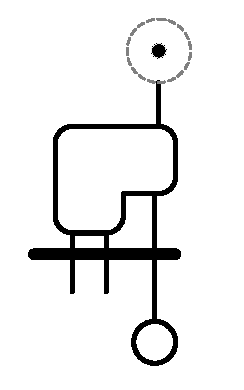
\includegraphics[width=.2\textwidth]{figures/Squiggle.pdf}
\end{center}  


% \vspace{2em}
\vspace*{\fill}

\noindent
\textsf{Last Compiled: \today}

\noindent
\textsf{Image: Birdtrack notation for tensor contraction}

\noindent
\textsf{CC BY-NC-SA 4.0}~\ccbyncsa 

\noindent % Course notes URL
% \url{https://github.com/fliptanedo/P231-2023-Math-Methods}

%% Front page logos
\vspace*{\fill}
\begin{center}

\includegraphics[height=.1\textwidth]{figures/FlipAmbigram.png}
\hspace{5em}

\includegraphics[height=.1\textwidth]{figures/UCRPnA_banner.png}
\end{center}

\newpage

\small
\setcounter{tocdepth}{2}
\tableofcontents
\normalsize
\clearpage
\restoregeometry        %% Return to lecture note geometry 
\pagenumbering{arabic}  %% Turn on regular page numbers


%%%%%%%%%%%%%%%%%%%%%
%%%  THE CONTENT  %%%
%%%%%%%%%%%%%%%%%%%%%

%% TEMPLATE STUFF
% %!TEX root = lecturenotes.tex
%% Update the above with the appropriate root

\chapter{Margins and Figures} %% if using report class

The main difference between my lecture notes and my paper template is the large margin to make use of side notes. The margin is a natural place to encourage students to jot notes and to host useful marginalia.%
\begin{marginfigure}%[th]
    \includegraphics[width=.8\textwidth]{example-image-golden}
    \captionsetup{font={scriptsize,sf}}
    \caption{Example of a margin figure.}
    \label{fig:figure:example:golden}
\end{marginfigure}
You can even place figures in the margin, see Fig.~\ref{fig:figure:example:golden}.\sidenote{Look! No float collision!}

\section{Vision}

This document is inspired by Edward Tufte and the implementation of his ideals in the \texttt{tufte-latex} package. The notes have a large margin for side notes and floats (e.g.\ figures).  Visually this means that the column of main text is narrower, which permits a slightly smaller font.


\section{Using the Margin}

We implement marginalia with the \texttt{sidenotes} package\index{side notes}. We highlight the main usage here. A standard sidenote uses \verb!\sidenote{...}! and looks like this\sidenote{Test of a sidenote. Let's add some extra text here to demonstrate the following point about non-overlapping notes}. Unlike \verb!marginnote!s, \verb!sidenotes! do not overlap with each other.\sidenote{An example of a sidenote that does not overlap with the previous one.} What more, the sidenotes coexist fine with footnotes.\footnote{Here is a foot note.}.

\paragraph{Figures} You can place entire figure floats in the main text region or in the margin. Fig.~\ref{fig:figure:example:golden} is a good example.

All we did was take \texttt{figure}$\rightarrow$\texttt{marginfigure}. You can do the same thing with \texttt{margintable}. On the other hand, sometimes you want a figure that spans the entire text width. Or, perhaps, you want several figures next to each other for comparison. To do this, we simply use the \texttt{figure*} environment. We demonstrate this in Fig.~\ref{fig:subfigure:example:lec}.
\begin{figure*}%[th]
    \centering
    \begin{subfigure}{0.3\linewidth}
    \centering
        \includegraphics[width=\linewidth]{example-image-a}
        \caption{First subfig}
        \label{fig:subfig:1:lec}
    \end{subfigure}\;%
    \begin{subfigure}{0.3\linewidth}
    \centering
        \includegraphics[width=\linewidth]{example-image-a}
        \caption{Second subfig}
        \label{fig:subfig:2:lec}
    \end{subfigure}\;%
    \begin{subfigure}{0.3\linewidth}
    \centering
        \includegraphics[width=\linewidth]{example-image-a}
        \caption{Third subfig}
        \label{fig:subfig:3:lec}
    \end{subfigure}%
    % \captionsetup{font={footnotesize,sf}}
    \caption{Here's how to spread a figure across the entire page, not just the main text width.}
    \label{fig:subfigure:example:lec}
\end{figure*}


We can place large figures in the main text and then place the figure caption in the margin notes. Compare the subfigure in Fig.~\ref{fig:subfig:3:lec} of Fig.~\ref{fig:subfigure:example:lec} to Fig.~\ref{fig:figure:example:golden:sidecap}.
\begin{figure}%[th]
    % \centering
    \sidecaption[][-2\baselineskip]{%
        Example of a margin figure. Note that the \texttt{label} command must be inside the \texttt{sidecaption}. (See source.)
        %
        %% \label command inside the \sidecaption command
        \label{fig:figure:example:golden:sidecap}
    }
    \includegraphics[width=\textwidth]{example-image-golden}
\end{figure}

\section{Other types of marginalia}

Sometimes you can use \texttt{marginnote} to place a note without a marking.\marginnote{See?} Note that \texttt{marginnote} does not, by default, use the same font as \texttt{sidenote}, so we had to set this in the preamble (\texttt{FlipLectureMacros.tex}).


Maybe we want to put another type of float in the margin?
What about a table, like Table~\ref{tab:margin:Table}?
% 
\begin{margintable}[-1em]
\small
    \begin{tabular}{ @{} llll @{} } \toprule % @{} removes space
        Element 
        & Core
        & Mantle
        % & $C_\text{cap}^N (\text{s}^{-1})$ 
        \\ \hline
        Iron 
        & 0.855 
        & 0.0626 
        % & $9.43\times 10^{7}$ 
        \\
        Nickel 
        & 0.052 
        & 0.00196 
        % & $7.10\times 10^{6}$ 
        \\
        Silicon 
        & 0.06 
        & 0.210 
        % & $2.24\times 10^{6}$ 
        \\
        Magnesium 
        & 0 
        & 0.228 
        % & $1.05\times 10^{6}$ 
        \\ \bottomrule
    \end{tabular}
    \captionsetup{font={scriptsize,sf}}
    \caption{Example of a margin table.}
    \label{tab:margin:Table}
\end{margintable}
One curious thing is that \texttt{margintable} does not float independently like a \texttt{sidenote}. Just be a bit careful using this since sometimes it requires manual spacing.
Another curiosity is that in my setup \texttt{sidefigure} and \texttt{sidetable} from the \texttt{sidenotes} package do not seem to work. I think may be because I played around a bit to try to make the \texttt{sidenote} font uniform.

\section{Breaking the Margin}


We define an environment \texttt{wide}\index{wide} that allows text, like equations, to spill into the margins. For example:
\begin{wide}
\begin{align}
f &= \sin\mleft(\frac{x^2}{2}\mright)
\times \arctan t 
\times \log \mleft(\cos \theta\mright)
\times \int_a^b \D{}x \exp\mleft(a^1 + b^2 + x^2\mright)
\times e^{-i\pi} 
\times \Gamma(n) 
\times _{n\!}\text{C}_m
\end{align}
\end{wide}
\begin{wide}
The definition of the margin spillover in \texttt{wide} needs to be matched to the size of the margin defined with the \texttt{geometry} package. Here's what normal text looks like.  The user must be responsible not to place any sidenotes while inside the \texttt{wide} environment.
\end{wide}


\section{Subsequent side notes}

One reason we use \texttt{sidenotes} instead of \texttt{marginnotes} is that \texttt{sidenotes} treats the notes as floating environments that do not overlap with one another.\sidenote{Here is a side note.} These side notes may cause warnings, but should not overlap.\sidenote{Here is another side note that should not overlap.}

Here's a sentence with some citations.\sidenote{Let's make this work. $\e^{i\pi} = -1$.}



\section{Some common environments}

\begin{theorem}[Euler's Identity]
\label{thm:euler:identity}
    Euler's identity\index{Euler's identity} is
    \begin{align}
        \e^{i\pi} = -1 \ .
    \end{align}
    Note that we use the macro \verb!\e! for an upright $\e$ rather than an italicized $e$.
\end{theorem}

\begin{exercise}
\label{ex:derive:euler:identity}
    Derive Euler's identity, Thm.~\ref{thm:euler:identity}.
\end{exercise}

\noindent Good students\index{good students} do the exercises, like Exercise~\ref{ex:derive:euler:identity}. Good instructors provide lots of examples, like Example~\ref{eg:easy:example}.

\begin{example}
\label{eg:easy:example}
    Consider the geometric series
    \begin{align}
        S = \sum_{n=0} a^n \ .
    \end{align}
    We can find a closed form expression for $S$ using
    \begin{align}
        S - aS &= 1\\
        S &= \frac{1}{1-a} \ .
    \end{align}
\end{example}

\section{Some specialized environments}

\begin{bigidea}[Principle of Easy Examples]
\label{idea:easy:examples}
The examples in a book are typically much simpler than the exercises.\sidenotemark
\end{bigidea}\sidenotetext[][-2.4em]{Don't you hate it when this happens?\label{sidenote:in:environment}}

\noindent  Notice that \bigidearef{}~\ref{idea:easy:examples} has a sidenote. Ordinarily \verb!\sidnote{}! does not work in environments. To hack this manually\sidenote{And only do this sparingly!} one may use \verb!\sidenotemark! inside the environment to place the marking and then 
\begin{quotation}
\verb!\sidenotetext[][-2cm]{sidenote}!
\end{quotation}
to implement the sidenote with a manual vertical adjustment.



\section{References}

We use \texttt{biblatex} (not \BibTeX{}) to place references as footnotes.\sidenote{Unlike \BibTeX{}, biblatex does not have a fancy logo. It is simple to make one up: \BibLaTeX{}.} This is because in pedagogical material, you \emph{want} readers to engage with references. Thus it makes sense to put the reference on the same page that you refer to them rather than sequestered at the end of a chapter or---worse---the end of the document. Here is a test citation using \texttt{autocite}: some paper.\autocite{Feng:2016ijc} What is nice is that \BibLaTeX{} is clever with repeated citations.\autocite{Feng:2016ijc} Notice how it does not dump all of the bibliographic data, just what you need to remember the paper and a hyperlink to the original footnote with the full reference. It even takes \texttt{arXiv} identifies with no additional modification.


% \chapter{Paper examples}

% Here are the standard examples I use for my \texttt{paper} template. I include them here to check that nothing has broken. These do not make use of the margin at all. You can see what happens when some text spills into the margin unintentionally.

% %!TEX root = paper.tex
%% Update the above with the appropriate root

\section{Common environments}

\subsection{Figures: floating and wrapped}

\begin{figure}%[th]
    \centering
    \includegraphics[width=0.4\textwidth]{example-image-a}
    \caption{The figure environment shows up often.}
    \label{fig:figure:example}
\end{figure}


\begin{figure}%[th]
    \centering
	\begin{subfigure}{0.3\textwidth}
    \centering
        \includegraphics[width=\linewidth]{example-image-a}
        \caption{First subfig}
        \label{fig:subfig:1}
    \end{subfigure}\;%
    \begin{subfigure}{0.3\textwidth}
    \centering
        \includegraphics[width=\linewidth]{example-image-a}
        \caption{Second subfig}
        \label{fig:subfig:2}
    \end{subfigure}\;%
    \begin{subfigure}{0.3\textwidth}
    \centering
        \includegraphics[width=\linewidth]{example-image-a}
        \caption{Third subfig}
        \label{fig:subfig:3}
    \end{subfigure}%
    \caption{Here's how to use subfigures}
    \label{fig:subfigure:example}
\end{figure}

Use 
% \textbackslash\texttt{centering}
\verb!\centering!
rather than the \texttt{center} environment in figure environments to avoid adding extra vertical space.\footnote{\url{https://tex.stackexchange.com/a/23653/8094}\label{foot:centering}}

\begin{wrapfigure}{l}{0.3\textwidth}
	\includegraphics[width=0.9\linewidth]{example-image-a}
	\caption{via \texttt{wrapfigure}.}
	\label{fig:wrapfig}
\end{wrapfigure}
\lipsum[1]

\subsection{Figures in Equation Environments}
\label{sec:figs}

\begin{align}
	\vcenter{
		\hbox{\includegraphics[width=.1\textwidth]{{example-image-a}}}
		}
	&=
	i g \gamma^\mu \ . 
	\label{eq:vector}
	\\
	\vcenter{
		\hbox{\includegraphics[width=.1\textwidth]{{example-image-a}}}
		}
	&=
	g \gamma^\mu\gamma^5 \ . 
	\label{eq:axial}
	\\
	\vcenter{
		\hbox{\includegraphics[width=.1\textwidth]{{example-image-a}}}
		}
	&=
	ig  \ . 
	\label{eq:scalar}
	\\
	\vcenter{
		\hbox{\includegraphics[width=.1\textwidth]{{example-image-a}}}
		}
	&=
	g \gamma^5 \ . 
	\label{eq:pseudo}
\end{align}


\subsection{Best practices for tables}
\label{sec:tables}

% \begin{table}
	% \renewcommand{\arraystretch}{1.3} % spacing between rows
	% \centering
	\begin{tabular}{ @{} llll @{} } \toprule % @{} removes space
		Element 
		& Core MF 
		& Mantle MF 
		& $C_\text{cap}^N (\text{s}^{-1})$ 
		\\ \hline
		Iron 
		& 0.855 
		& 0.0626 
		& $9.43\times 10^{7}$ 
		\\
		Nickel 
		& 0.052 
		& 0.00196 
		& $7.10\times 10^{6}$ 
		\\
		Silicon 
		& 0.06 
		& 0.210 
		& $2.24\times 10^{6}$ 
		\\
		Magnesium 
		& 0 
		& 0.228 
		& $1.05\times 10^{6}$ 
		\\ \bottomrule
	\end{tabular}
	% \caption{
		% Mass fractions of the Earth's core and mantle.
		% \label{table:elements}
% 	}
% \end{table}




\section{Labels and cleveref}
\label{sec:labels:and:cleveref}

\subsection{\texorpdfstring{\texttt{cleveref}}{cleveref}}
\label{sec:cleveref}

\texttt{cleveref} is a handy package when referring to ranges of equations. 

The pseudoscalar rule is:
\begin{itemize}
	\item Using \texttt{amsmath.sty}'s \texttt{eqref}: \eqref{eq:pseudo}
	\item Using \texttt{cleverefs}'s \texttt{cref}: \cref{eq:pseudo}
\end{itemize}

The equations above are
\begin{itemize}
	\item Using \texttt{amsmath.sty}'s \texttt{eqref}: \eqref{eq:vector} -- \eqref{eq:pseudo}
	\item Using \texttt{cleverefs}'s \texttt{crefrange}: \crefrange{eq:vector}{eq:pseudo}
\end{itemize}

The equations above are (glomped together)
\begin{itemize}
	\item Using \texttt{amsmath.sty}'s \texttt{eqref}: \eqref{eq:vector}, \eqref{eq:axial}, \eqref{eq:scalar}, \eqref{eq:pseudo}
	\item Using \texttt{cleverefs}'s \texttt{cref}: \cref{eq:vector,eq:pseudo,eq:axial,eq:scalar}
\end{itemize}

\texttt{cleveref} automatically identifies the type of object it is referring to. Thus you can use \verb!\cref! to refer to any label, for example \cref{foot:centering}. You can use \verb!\Cref! to have a capitalized the cross reference name. For example: the sections above are \Cref{sec:macros,sec:cleveref,sec:figs,sec:tables}.


\subsection{Sub-equations}

One can also wrap a \texttt{align} environment with a \texttt{subequations} environment. The \texttt{subequations} environment can be given a label. For example,
\begin{subequations}\label{eq:subequations}
\begin{align}
	a &= \pi 
	\label{eq:subequation:1}
	\\
	b &= \e^{\I \pi} 
	\ .
	\label{eq:subequation:2}
\end{align}
\end{subequations}
where we can now refer to the pair of equations \eqref{eq:subequations} or simply one of the equations, \eqref{eq:subequation:2}. This also works in \texttt{cleveref}: \cref{eq:subequations} and \cref{eq:subequation:2}.


\subsection{Referring to Equations}

One style suggestion is to use parentheses to refer to an equation with no additional modifiers \emph{except} at the beginning of a sentence.\footnote{\url{https://academia.stackexchange.com/a/21793}} For example: ``The second term in (3)...'' and ``Equation~(3) has two terms...''



\section{Macros}
\label{sec:macros}


\subsection{Modest capitalization}

Small caps are useful when your text contains acronyms and you do not want them to visually imply emphasis. In other words, we can use them as `not shouting' capitalization. We define a macro \texttt{acro} for this purpose. The default is for \texttt{acro} to be a wrapper for \texttt{small}. Here is an example:
\begin{itemize}
	\item \acro{AdS} in \acro{5D} at the \acro{LHC}.
	\item AdS in 5D at the LHC. 
	\item A third list item to test list spacing.
\end{itemize}


\subsection{Macros for Collaboration}

There are many ways to add notes when collaborating on a document. I like in-line notes with an author name and a color.  \flip{This is an example of a comment.} It is also useful to have a macro for highlighting new text and for proposing the removal of old text.\footnote{Git does this automatically at the level of source code. \texttt{LaTeXDiff} ostensibly does this automatically, but is prone to compile errors and is notoriously difficult to troubleshoot.}

\new{
I fixed the equation:
\begin{align}
	a=b^2 
	\label{eq:samename}
\end{align}
It has label \texttt{eq:samename}. 
}

\remove{
	% It is good practice to indent the `to-be deleted' text
	Here is an equation:
	\begin{align}
	a=b 
	\label{eq:samename}
	\end{align}
	It has label \texttt{eq:samename}.
}

This is essentially a manual version of the \texttt{latexdiff} command. This command can be notoriously fussy around math environments. I personally advocate for using \texttt{git}-related tools to quickly identifying where a version was edited and then using tags to identify edits that need to be highlighted for further discussion. One nice thing about the \texttt{remove} tag above is that it also strips any \texttt{label}s so that there are no `multiply defined label' warnings and one can uniquely refer to a single equation, \eqref{eq:samename}.

\begin{flipcomment}
This is an extended comment that shows up as a text box. I might use this to make some ponderous point about why I think my version of a draft paragraph is more appropriate than yours.
\end{flipcomment}


\subsection{\texorpdfstring{\texttt{xspace}}{xspace}}

The \verb!\xspace! command is useful at the end of a macro. It stands for: ``insert a space if and only if there is supposed to be a space.'' Consider the following examples:
\begin{itemize}
	\item Without \texttt{xspace}: \LaTeX typesetting...
	\item With \texttt{xspace}: \LaTeX\xspace typesetting...
	\item Without \texttt{xspace}: Typeset with \LaTeX.
	\item With \texttt{xspace}: Typeset with \LaTeX\xspace.
\end{itemize}
However, one should consider \verb!\xspace! depreciated. It can be useful for spacing with user-defined macros. However, the results can be unreliable.\footnote{\url{https://tex.stackexchange.com/a/86620/8094}}  For example, one could define \verb!\newcommand{\test}{{test}\xspace}!, note the extra pair of braces in the definition. Even though there is an \verb!\xspace!, this command will fail to place a space between \verb!\test \test!. This type of problem shows up for me because I have a macro \verb!\acro{}! for making acronyms smaller. If I define a shortcut \verb!\newcommand{\DM}{\acro{DM}}! then there is no space between \verb!\DM \test!. The result is: \acro{DM}\xspace {test}. 

The suggested practice is to end your commands with empty braces or a slash: \verb!\DM{}! or \verb!\DM\!. All spacing works out as intended. 
\begin{itemize}
	\item \verb!\DM{} Halo! produces \DM{} Halo
	\item \verb!\LaTeX Fails.! produces \LaTeX Fails.
	\item \verb!\LaTeX{} Works.! produces \LaTeX{} Works.
\end{itemize}






\section{Mathematics and Physics}

\subsection{Environments}

Use the \texttt{align} environment instead of \texttt{eqnarray}, see the TeXblog discussion\footnote{\url{https://texblog.net/latex-archive/maths/eqnarray-align-environment/}}. The double dollar sign notation for \texttt{displaymath} is depreciated.\footnote{\url{https://tex.stackexchange.com/questions/503/why-is-preferable-to}} The suggested alternative is \verb!\[! and \verb!\]!, though this is rather annoying. As a default I always use \texttt{align}.

Single dollar sign \verb!$! notation is also depreciated relative to \verb!\(! and \verb!\)! for inline text. However, I am stubborn about keeping in-line text as simple as possible. The dollar sign is a single character and it is visually easier to identify as a delimiter for math mode. I thus continue using single dollar signs for inline mathematics. 


\subsection{Text and Math: super- and subscripts}

Use the \texttt{text} command to insert text into math environments. For subscripts use \texttt{textnormal}. 
% 
We use the \texttt{textnormal} command for super- or subscripts rather than the \texttt{text} command because this automatically uses the correct size. Compare, for example: $G_\textnormal{D},\, G_\text{D}$.

One place this shows up is if you have a subscript that is not a mathematical variable. For example, $x_a$ makes sense for the value of $x$ at point $a$, but $x_\text{b}$ should be used if the `b' is shorthand for boundary. Similarly, $E_\text{max}$ for the maximum energy, rather than $E_{max}$.


\subsection{Units and spacing}

Use a tie (tilde) to enforce a non-breaking short space between a number and its units: $0.5~\text{MeV}$. Units should not be italicized. If you want to be svelte you can use a thin space, \verb!\,!. Some people like the \texttt{siunitx} package; I find it a little cumbersome for that it is, especially given that I usually write in natural units.

Some care is required for spacing with math operators\footnote{\url{https://tex.stackexchange.com/a/35585/8094}}. Here's a guideline for how to use different bits of manual spacing\footnote{\url{https://tex.stackexchange.com/questions/25810/when-one-should-use-spacing-line-quad-or}}.


\subsection{Upright characters}

These come from the \acro{ISO 80000} standards for typesetting mathematics and physics.\footnote{See discussion in \url{https://tex.stackexchange.com/q/14821/8094}} It is not obvious to me that these are applicable to the typographical culture of physics, but the most important thing is to be consistent.
\begin{itemize}
	\item Units are always upright, \textmu m is a micrometer. You can use various unit packages to do this automatically. 
	\item The base of the natural logarithm is upright $\e^{i\pi}$ versus $e^{i\pi}$. The best physics argument is to avoid confusion between the exponential $\e$ and the electric coupling $\alpha = e^2/4\pi$.\footnote{I thank Matt Reece for pointing this out to me.}
	\item The differential is an operator so it should be upright. I have macros for this: $dx$ vs.~$\D{x}$ and $\dbar p$ vs.~$\Dbar{p}$. The \texttt{physics} package has macros for this. 
	\item You could also do this for the imaginary number: $a+\I b = \e^{\I \theta}$. This one is a little trickier to get the spacing right. We use \verb!\newcommand{\I}{\operatorname{i}\mkern-2mu}!.
	\item You can use \verb!\DeclareMathOperator! to define upright Roman letters that should be treated as a single operator like $\sin$. This also automatically fixes the spacing after the operator contextually depending on whether the next character is understood as an argument, $\sin x$, or a group $\sin(ax)$.
\end{itemize}
There is a historical discussion on \texttt{hsm.stackexchange}\footnote{\url{https://hsm.stackexchange.com/questions/6727/fracdydx-versus-frac-mathrm-dy-mathrm-dx}}.  For all of these, it helps to define macros. This makes it easy to change the style when you have a co-author who strongly disagrees.

\subsection{Absolute Values}

We define a macro \verb!\abs{}! to invoke \texttt{amsmath}'s \verb!\lvert! and \verb!\rvert! commands for automatically sizing the left- and right-bars of an absolute value. Examples:
\begin{align}
	\abs{x} &&
	\abs{\frac{x}{y}} &&
	\abs{\int \D{x} \, e^{i px}} &&
	\int \D{x} \, \abs{e^{i px}}
	\ .
\end{align}
If you want to be fancier, you can use \texttt{mathtools}\footnote{\url{https://tex.stackexchange.com/a/35585/8094}} to define custom delimiters. For example:
\verb!\DeclarePairedDelimiter{\abs}{|}{|}! \, .


\subsection{Miscellaneous}

\begin{itemize}
	\item Use $\mid$ instead of pipe for conditions: $p(x\mid y)$ versus $p(x|y)$.
	% 
	\item Transpose: The \acro{ISO}~80000 standard has suggestions. $A^T$ vs $A^\top$ vs $A^{\trans}$. I personally prefer $A^\text{T}$.
	% 
	\item \textbf{Textual subscripts}: sometimes you have a subscript that is not an index, but shorthand for something textual. For example, the Green's function with Dirichlet boundary conditions is $G_\textnormal{D}$. The subscript is upright, not italicized, $G_D$. Use the \texttt{textnormal} command rather than the \texttt{text} command since this will automatically use the correct size. Comparison: $G_\textnormal{D},\, G_\text{D}$.
	% 
	\item Arrows with text under them: \texttt{xrightarrow} in the \texttt{amsmath} package. The square bracketed argument is under, the curly bracketed argument is over. Example: $\xrightarrow[\textnormal{low}]{\textnormal{hi}}$.
	% 
	\item We can use the $\defeq$ symbol, defined as a macro\footnote{\url{https://tex.stackexchange.com/a/4881/8094}} \verb!\defeq!, to denote assignment . The macro typesets the symbol so that the dots are the same size and aligned with the lines. In pedagogical writing, it may be useful to distinguish between equality $=$, assignment $\defeq$, and tautology $\equiv$. At least that is how I use these.\footnote{Arnold Arons brings up equal signs in \emph{Teaching Introductory Physics}, Chapter~3.23. I prefer $\defeq$ for definitions because it shows the asymmetry of the relation. The statement $a\defeq b$ means that $a$ is defined to be $b$. The equal sign $=$ is symmetric in appearance and in meaning: $a$ and $b$ are the same. I use  $a\equiv b$ sparingly to mean $a$ and $b$ are \emph{obviously} the same but in a way that is not necessarily derived mathematically. }
\end{itemize}



\section{Space}

\subsection{Kerning: spacing between characters}
Math operators have a natural spacing before and after depending on the context. In the following example, spaces indicate that the coefficient $a$ multiplies the logarithm of $b$:
\begin{align}
	a\log b && a\log(bc)
\end{align}
The space on either side of $\log$ indicate that $\log$ is a mathematical operator. The second example still has the space between $a$ and $\log$, but has no space between $\log$ and $(bc)$ because the parenthesis belongs to the mathematical function.\footnote{Example from \url{https://tex.stackexchange.com/a/140647}}
% 
You can use \verb!\DeclareMathOperator! for functions that are not built in.

Using \verb!\left(! and \verb!\right)! will automatically size parentheses, but can mess up kerning:
\begin{align}
	f(x)
	f\left(x\right)
	f{\left(x\right)}
	&
	&
	\cos(x)
	\cos\left(x\right)
	\cos{\left(x\right)}
	{\cos}{\left(x\right)}
	\ .
\end{align}
The crude way to fix this is to put braces around the parentheses: \verb!{\left(x\right)}!.\footnote{\url{https://tex.stackexchange.com/a/2610/8094}}. However, if the parenthesis is attached to a mathematical operators, the operator must also be surrounded by braces: \verb!{\cos}!. In the examples above, you can see the effect of the braces on the spacing on either side.



\subsection{Manual Spacing}

\LaTeX{} has commands for manually inserting spacing: 
\begin{itemize}
	\item \verb!\,! thin\,space
	\item \verb!\:! medium\:space
	\item \verb!\;! thick\;space
	\item \verb$\!$ thin\!negative\!space.
		  %% note the use of a different symbol in \verb 		
\end{itemize}
The negative space can be helpful for manually adjusting the kerning for large parentheses raised to a power:
\begin{align}
	\left(\frac{\pi}{\sum_{i=1}^n x^i}\right)^{d+1}
	&&
	\left(\frac{\pi}{\sum_{i=1}^n x^i}\right)^{\!d+1}
	\ .
\end{align}
On the right we use \verb$\right)^{\!d+1}$.



\subsection{Ties create non-breaking spaces}

\LaTeX{} interprets periods as full stops (end of a sentence). It places extra space after the full stop. Use a \textbf{normal space} right after the period, \verb!.\ ! (``slash space'') to tell \LaTeX{} that a period is not a full stop and that it should insert insert a normal space not a double space.\footnote{The double space is sometimes considered old fashioned. You can use \texttt{frenchspacing} in your document to turn off the double space after a full stop.} Mr.\ Roboto versus Mr. Roboto. 


% Use a \textbf{tie} (tilde) when a period is not a full stop: Mr.~Roboto versus Mr. Roboto. 
A related construction is a \textbf{tie} (tilde). This gives \textbf{non-breaking space} which is a normal space that \LaTeX{} interprets as `part of the word'. This means that line breaks should not occur along the non-breaking space.
% 
You can also use ties this whenever you want to prevent a line break between words. \LaTeX{} interprets the tied words as a single word.
% 
Ties are also standard for citations: \verb!Tanedo et al.~\cite{citation}!. 




\section{Some Best Practices}

\subsection{\texorpdfstring{\LaTeX{} in a title}{LaTeX in a title}}

When using \LaTeX{} code in a section title, use the \texttt{texorpdfstring} command to define an \acro{UTF-8} string that the pdf can use for bookmarks. If you do not do this, there are annoying compilation warnings.


\subsection{Ranges}

Hyphens, en dashes, em dashes, and minus signs in math mode are all grammatically different.
\begin{itemize}
	\item En dashes replace hyphens in a compound adjective where one of the elements is a two-word compound: `post--Cold War era.'\footnote{From \url{https://www.merriam-webster.com/words-at-play/em-dash-en-dash-how-to-use}}
	\item En dashes are used for combinations of two names in place of the word `and.' For example, Randall--Sundrum model.
	\item For compound names of a single person, use a hyphen: Levi-Civita.
	\item A minus sign should be typeset in math mode, $-1$.
\end{itemize}
The choice between a hyphen and en dash can be tricky. For example \acro{APS} seems to prefer ``anti--de Sitter'' with an en dash, whereas others prefer a hyphen.\footnote{See 1 Jan '23: \url{https://en.wikipedia.org/wiki/Talk:Anti-de_Sitter_space}.}


\subsection{References}

Use \BibTeX\xspace. There are any number of \BibTeX\xspace managers. One that I like is Yuji Tachikawa's \texttt{spires.app}\footnote{\url{https://member.ipmu.jp/yuji.tachikawa/spires/}}; it links directly to the inSpire \acro{HEP} database. For styling, I recommend Jacques Distler's \texttt{utcaps.bst} which is a nice format that automatically inserts a hyper link to the \texttt{arXiv} version of a paper. If yo are fancy you may use {\rm B\kern-.05em{\sc i\kern-.025em b}\LaTeX{}. 


Standard citation managers with \BibTeX\xspace capability make a big deal about assigning unique \BibTeX\xspace citation keys to each reference. This can be tedious if you have to collaborate with someone else who has made up their own citation keys. Fortunately, in my field there is a single recognized database, inSpire\footnote{\url{https://inspirehep.net}; see also \acro{NASA/ADS} for astronomy.}, that assigns a unique \BibTeX entry for papers.  This means that it is good practice to select keys as follows:
\begin{itemize}
	\item If it exists, use the inSpire key. Tools like \texttt{spires.app} default to this key.
	\item If inSpire does not have the reference, use \acro{NASA/ADS}.
	\item If neither of those databases has the references, find a simple algorithm that all of your coauthors can agree upon. 
\end{itemize}
Items in the third category are usually books and websites. 



\section{Neat examples}

Suppose you would like to repeat and equation reference,
\begin{align}
	\e^{\I\pi} &= -1 
	\ .
	\label{eq:e:ipi}
\end{align}
Remember that equation above? Let's write it again,
\begin{align}
	\e^{\I\pi} &= -1 
	\ .
	\tag{\ref{eq:e:ipi}}
\end{align}
Observe that these have the same equation number. Instead of \texttt{label} we use \texttt{tag} with argument \texttt{ref}.

% %!TEX root = paper.tex
%% Update the above with the appropriate root

\section{Teaching Examples}

For lecture notes it is useful to have some framed environments to highlight examples and exercises. In the past I have used \texttt{framed} and \texttt{mdframed}. I think \texttt{tcolorbox} may be the best option now.

% \begin{tcolorbox}
% 	⟨environment content⟩
% \end{tcolorbox}

\begin{theorem}[Flip's Theorem]
This is an example theorem.
\end{theorem}

\begin{example}[Flip's Example]
This is an example of an example
\end{example}


\begin{exercise}[Solving a differential equation]
  Solve the following differential equation.
  \label{ex:solve:ode}
\end{exercise} 
\noindent Can you solve Exercise~\ref{ex:solve:ode}?


\begin{bigidea}[environments]
  With \texttt{tcolorbox}, one may `dress' existing environments in boxes. The call to the environments is unchanged.
  \label{idea:environments}
\end{bigidea} 
\noindent Refer to \bigidearef{}~\ref{idea:environments}.
% %!TEX root = paper.tex
%% Update the above with the appropriate root

\section{Code example}

These are examples of the \texttt{listings} package for typesetting code. See Overleaf\footnote{\url{https://www.overleaf.com/learn/latex/Code_listing}} and \acro{TeX.SE}~\footnote{\url{https://tex.stackexchange.com/a/350242}} for more information. By the way, printed out code is called `listings' because old computer languages has a \texttt{LIST} command to print out the numbered source code lines.\footnote{\url{https://softwareengineering.stackexchange.com/a/289729}}

\subsection{Inline}

If you just want to be able to insert \LaTeX{} into a document like this, you can use \verb!\verb!\footnote{\url{https://stackoverflow.com/a/66115768/16426341}}. The way it works is that you write \verb!\verb#TEXT#! where \verb!#! is any character that is not in \texttt{TEXT}. You can use listings package similarly with \verb!\lstinline! in place of \verb!\verb!.


\subsection{Jupyter Notebook}

Jupyter formatting from user \texttt{yogabonito} on \acro{TeX.SE}\footnote{\url{https://tex.stackexchange.com/a/350242/8094}}.

\begin{pyin}%[pyin01]
print("Hello world")
\end{pyin}
%  
\begin{pyprint}
Hello world
\end{pyprint}
% 
You get a `multiply defined label' warning if you do not explicitly label each of your Python inputs. 
%% EXAMPLE: 
% \begin{pyin}
% print("Hello world, too")
% \end{pyin}
% \begin{pyin}
% print("Hello world, three.")
% \end{pyin}
%% This gives two Python inputs with label `' (blank)
%% and thus returns a compiler warning.
% 
% 
Here we have a return value in the last line of the input cell.
\begin{pyin}[labelOfTheSecondInput]
def twicify(arg):
    print("Received:", arg, "- Will double now...")
    return 2 * arg
twicify(1)
\end{pyin}

\begin{pyprint}
Received: 1 - Will double now...
\end{pyprint}

\begin{pyout}
2
\end{pyout}
% 
% \subsection{Referencing input}
You can also reference the labeled input \ref{labelOfTheSecondInput}, from above.
% \begin{pyin}[anotherlabel]
% "and the counter will automatically do the right thing :)"
% \end{pyin}
% \begin{pyout}
% 'and the counter will automatically do the right thing :)'
% \end{pyout}


\subsection{\texorpdfstring{\LaTeX}{LaTeX}}

From user \texttt{hair-splitter} on \acro{TeX.SE}\footnote{\url{https://tex.stackexchange.com/a/637305/8094}}:

\begin{lstlisting}[style=latexstyle]
\documentclass{article}
\usepackage[T1]{fontenc}
\newcommand*{\mycommand}{Hello World!}
\begin{document}
  \mycommand
\end{document}
\end{lstlisting}


% %!TEX root = paper.tex
%% Update the above with the appropriate root

\section{\texorpdfstring{\LaTeX{} Style}{LaTeX Style}}

There is not a definitive \LaTeX{} style guide analogous to \acro{PEP-8}. However, I do have my own set of preferences. Here style refers to how the \LaTeX{} source files are written. Two \texttt{tex} files may produce identical \texttt{pdf} outputs but be stylistically different. A well styled document is that is as easy as possible to parse and edit as a human being. I have done my best to keep the source files for \emph{this} template well styled.


\subsection{Idiosyncracies}

While some coding style guides require a fixed width for the document. This gives meaning to a line of code and makes the resulting source more readable by avoiding unintentional text wrapping. \LaTeX{} is a bit different in that it is a typesetting language that is meant to handle paragraphs of text. Because modern editors naturally have text wrapping options, I do not feel strongly about enforcing a document-wide character width limit. Paragraphs of text should be allowed to wrap if that makes sense. However, mathematics environments should strive to make use of white space in service to readability.


\subsection{Spacing and Indents}

White space helps distinguish the document structure. 

\begin{enumerate}
	\item Sections should have three empty lines between each other.
	\item Sub-sections should have two empty lines between each other.
	\item All other units of paragraphs should have one empty line space between them.
\end{enumerate}
One may use with commented out empty lines to separate sentences from one another. 
% 
	This produces no paragraph break between the sentences in the output, but can help separate different ideas within a paragraph.
% 
	Similarly, one can combine this with indents to help visually organize the logical flow of a paragraph.


\subsection{Mathematics}

Use comments and white space to separate mathematics environments from plain text.
% 
The contents of a mathematics environment should use ample white space to separate each mathematical object as if these were words in a sentence.
% 
\begin{lstlisting}[style=latexstyle]
\begin{align}
  S_{\textnormal{fix}}^{\textnormal{Bulk}}
  & =
  \frac{-1}{g^2} 
  % \int d^{d+1} x  
  \int \DD{d+1}{x}
  \left( \frac{R}{z} \right)^{\!d-3}
  \frac{1}{2\xi}
  \left[
    \partial_\mu A^\mu
    -
    \xi\left( 
      z^{d-3} 
      \partial_z \left( \frac{A_z}{z^{d-3}} \right)
      -
      \left( \frac{R}{z} \right)^{\!2} 
      g^2 v(z) \, \pi
    \right)
  \right]^2 \ ,
\label{eq:SGFBulk}
\end{align}
\end{lstlisting}
% 
This produces the following:
\begin{align}
	S_{\textnormal{fix}}^{\textnormal{Bulk}}
	& =
	\frac{-1}{g^2} 
	% \int d^{d+1} x  
	\int \DD{d+1}{x}  
	\left( \frac{R}{z} \right)^{\!d-3}\frac{1}{2\xi}
	\left[
	    \partial_\mu A^\mu
	    -
	    \xi\left( 
	        z^{d-3} \partial_z \left(\frac{A_z}{z^{d-3}}\right)
	        -
	        \left(\frac{R}{z}\right)^{\!2} g^2 v(z)\, \pi
	    \right)
	\right]^2 \ ,
% \label{eq:SGFBulk}
\end{align}
For long expressions, each line should be a well-defined `unit' of the mathematical expression. When there are multiple `words' in an expression, add white space to delimit them. The use of indentation to group elements of the same level should be self explanatory.

For example, simple fractions do not need any white space, while more complicated fractions should provide some help:
% 
\begin{lstlisting}[style=latexstyle]
\frac{ 
	b_\mathcal{O}
}{
	\Lambda^{\Delta_\mathcal{O} - \frac{d}{2} - 1 }
} 
\end{lstlisting}
% 
This may seem like overkill, but in an expression with multiple fractions it is helpful to be able to quickly visually parse each piece of the expression.


\subsection{When (not) to use macros}

Use macros (\texttt{newcommand} or \texttt{renewcommand}) when there is an expression that you use often \emph{and that you may want to change in the future}. Perhaps you have a variable that needs to be used uniformly across a document, but whose specific symbol may change. Use a macro and make it easy to change that symbol without doing a find-and-replace. Macros are also useful for making \LaTeX{} source more readable by truncating a tedious series of commands. 

However, do not use a macro just because it will make your life easier in the moment. One good reason \emph{not} to use a macro is as a shortcut for defining an environment. There is a `old style' of source preparation where someone will define macros:
% 
\begin{lstlisting}[style=latexstyle]
\newcommand{\be}{\begin{equation}}
\newcommand{\ee}{\end{equation}}
\end{lstlisting}
% 
This seems like a shortcut because it saves you the trouble of writing
% 
\begin{lstlisting}[style=latexstyle]
\begin{equation}
	...
\end{equation}
\end{lstlisting}
% 
There is a narrow range of tech-savvy for which this `trick' is useful: one has to be sophisticated enough where typing in six characters rather than thirty-one characters will save significant time, but one must also be na\"ive enough to not use a text editor that can do (1) text expansions or (2) context-aware text highlighting. 
% 
This latter point is what can drive a collaborator crazy: some \LaTeX{} editors look for \textbackslash\texttt{begin}--\textbackslash\texttt{end} pairs to identify math mode and highlight text in a helpful way. Macros like \texttt{be} and \texttt{ee} screw this up and can lead to linter warnings. In summary, do not define macros to simplify environments.


\subsection{Labels}

Labels should be descriptive, even if that means that they labels become a bit lengthy. Each label should start with some indication of what it is labeling, \texttt{eq} for equation or \texttt{fig} for figure, for example. Use colons to separate words.
% 
\begin{lstlisting}[style=latexstyle]
\label{eq:Euler:formula}
\label{sec:introduction}
\label{sec:introduction:past:work}
\end{lstlisting}
% 
Many \LaTeX{} editors have intelligent autocomplete that makes it easy to insert references to past labels, so it does not take any more time to have a lengthy label. It does, however, save time if your labels are descriptive and easy to select from a drop-down menu. 


\subsection{Collaborative writing}

A key principle of \LaTeX{} source should be making the document collaboration-friendly. It is \emph{not} sufficient that your \LaTeX{} source compiles. Your code needs to be:
\begin{enumerate}
	\item \textbf{Readable}. Use white space in a consistent way to reflect the underlying structure of your document and your expressions. Use consistent spacing between sections and subsections. Use ample white space within an equation to make each piece easy to identify. 
	\item \textbf{Editable}. Collaborators should be able to fix typos without having to do a deep dive of your source ode. 
\end{enumerate}
Here's what you are allowed to sacrifice in order to meet these goals:
\begin{enumerate}
	\item Your source code does not need to be short. Nobody will print out our source file. An equation that typesets to a single line can be spread out over a dozen lines if it helps the reader parse the \LaTeX{}. 
	\item Your source code does not need to be confined to a single file. 
	\item Your figures should be in a separate folder. In this template we use:
% 
\begin{lstlisting}[style=latexstyle]
\graphicspath{{figures/}}
\end{lstlisting}
% 
	\item Your pose writing---that is, writing that is not in math mode---can also be broken up using empty lines (comment out the line to avoid starting a new paragraph) and white space in order to elucidate the structure.\footnote{This can be useful if you tend to write convoluted sentences. You can `diagram' your sentence so that you see how each clause fits together.}
\end{enumerate}

A good way to collaborate is to use \texttt{git}/\texttt{github} or {Overleaf}. Overleaf is fantastic for abstracting away all version control. However, savvy users with an Overleaf membership can connect to Overleaf documents using \texttt{git}. This gives you the best of both worlds: you may use your favorite \acro{IDE} or \LaTeX{} editor and your favorite \texttt{git} client to synchronize to an Overleaf document that your collaborators can edit through the web interface if they wish.\footnote{You may notice that there is a \texttt{gitignore.txt} file in this template. It is a copy of the \texttt{.gitignore} file used by \texttt{git}. The \acro{macOS} interface does not like it when users try to manipulate files named dot-something since it worries that you might be messing up an important system file. Thus I have included a text file with the contents of \texttt{.gitignore} for users who simply want to copy this template folder using \acro{macOS}. You should then rename \texttt{gitignore.txt} to \texttt{.gitignore} if you are using \texttt{git}. Alternatively, download this file as a template from \texttt{github} and ignore \texttt{gitignore.txt} altogether.  }

\subsection{\texorpdfstring{\LaTeX{} Style Guide}{LaTeX Style Guide}}

\begin{itemize}
	\item Use \texttt{hyperref}. Modern documents should be internally and externally hyperlinked. Clicking on a reference to an equation should bring the reader to that equation. Use a bibliography style that allows hyperlinks to the \texttt{arXiv}.
	\item In \emph{informal} documents like this, I refer to websites (usually Stack Exchange) with a footnote and a hyperlink:
	% 
\begin{lstlisting}[style=latexstyle]
...a great website.%
\footnote{\url{https://www...}}
\end{lstlisting}
	% 
	This avoids having to use \BibTeX for one-off references and makes the reference easily clickable. 
	% 
\end{itemize}


\subsection{Copy Editing Style Guide}

These are non-specific style points:

\begin{itemize}
	\item Footnotes go after punctuation.%
			\footnote{Like this.}
	\item Use whitespace to separate footnotes:
	% 
\begin{lstlisting}[style=latexstyle]
We now make an important%
  \footnote{
	Observe the comment and whitespace.
	There is no additional spacing between
	`important' and this footnote. }
point about style.
\end{lstlisting}
	%
	\item You may consider using \textbackslash\texttt{frenchspacing} in your document.\footnote{Hat tip to Eddie Kohler, \url{https://www.read.seas.harvard.edu/~kohler/latex.html}}
\end{itemize}


\subsection{Breaking the rules}

It is okay to break the style rules when doing so supports clarity. Sometimes it makes sense to throw in lots of extra white space to separate ideas.


\subsection{Cleaning Up}

Sometimes it is okay to leave a mess. You may want to preserve an old `verbose' version of your source files that has intermediate steps spelled out overly-pedagogically. You may find it useful to leave comments in the source files to remind yourself of the structure of your argument. These changes are preserved if you use version control, but sometimes you want the redundancy and convenience of having old text readily available. Just remember to go through your source code carefully to strip it of comments before submitting to a public repository like the \texttt{arXiv}.
% %!TEX root = paper.tex
%% Update the above with the appropriate root

\section{References}

\subsection{\texorpdfstring{\LaTeX{} Style}{LaTeX Style}}

\begin{itemize}
    \item Didier Verna, ``Towards \LaTeX{} coding standards.\footnote{\url{https://tug.org/TUGboat/tb32-3/tb102verna.pdf}; video: \url{http://zeeba.tv/toward-latex-coding-standards/}}'' 
    \item See also Philippe Beliveau's summary of Verna's piece.\footnote{\url{https://medium.com/@pbeliveau/latex-coding-standards-f82743b7866b}}
    \item Evan Chen, ``Evan's \LaTeX{} Style Guide.\footnote{\url{https://web.evanchen.cc/latex-style-guide.html}}''
    \item Eddie Kohler, ``LaTeX Usage Notes.\footnote{\url{https://www.read.seas.harvard.edu/~kohler/latex.html}}''
\end{itemize}


\subsection{Style Guides}

Most publications have a style guide, analogous to the well-known \acro{APA} style in social sciences. Checking for strict adherence to those guides have historically been the role of copy editors, though the number of published papers continues to grow with no obvious increase in resources for copy editing. 

\begin{itemize}
    \item There is an \acro{ISO} standard for typesetting mathematics and physics. As of 2023 it is \acro{ISO80000}.
    \item Strunk \& White, \emph{The Elements of Style}
    \item The \emph{Review of Modern Physics} style guide. 
\end{itemize}

\subsection{Typography References}

The standard typography reference is Robert Bringhurst's \emph{The Elements of Typographic Style}. 
The following references focus specifically on typography and \LaTeX{}.
\begin{itemize}
    \item Consistent typography on \acro{TeX.SE}\footnote{\url{https://tex.stackexchange.com/questions/29840/consistent-typography}}
    \item List of best practices references on \acro{TeX.SE}\footnote{\url{https://tex.stackexchange.com/questions/577/best-practices-references}}, including the list of obsolete packages and commands in \LaTeX{}~2e\footnote{\url{https://www.ctan.org/tex-archive/info/l2tabu/english/}}
    \item ``The Art of \LaTeX{},'' a list of guidelines from Fan Pu Zeng\footnote{\url{https://fanpu.io/blog/2023/latex-tips/}}
    \item Showcase of beautiful typography in \LaTeX{}\footnote{\url{https://tex.stackexchange.com/q/1319/8094}}
\end{itemize}



% %% CHAPTER SUBAPPENDIX %% if using report class
% \begin{subappendices}
% \section{Subappendix}\label{sec:subappendix:eg}
% This chapter has its own special appendix.
% \end{subappendices}


\chapter{Introduction}

\section{Two powerful questions}
At any time in this course, you should feel comfortable asking either of the following questions:
\begin{enumerate}
    \item Is it obvious that...?
    \item Why is this significant?
\end{enumerate}
The first question is the way to ask for on-the-spot clarification---I will either appreciate that I did not properly explain a subtle point, \emph{or} I will explain the intuition\sidenote{Your sense of mathematical and physical intuition is incredibly valuable. This is one of the key traits that makes a physics training unique.} for why something should be obvious. The second question is a way to remind me that I may have \emph{lost sight of the forest for the trees}: I want this course to \emph{mathematically connect big ideas in physics}. Asking this question is a reminder that making those connections justifies the hard mathematical work we will put into the course.

\section{Exercises and Examples}
I have tried to insert exercises and examples in these notes. There are still far too few for sound pedagogy. If you really, really want to learn something, you \emph{have} to do exercises. Think of the examples as exercises with solutions---though they are not always written this way. Mull over the exercises: ask yourself why the problems are posed the way they are, challenge the statements to find the domain of validity, think of how one may extend those exercises to other applications. The exercises are a far better gauge of you learning than whether or not you have read a section of the notes. If you are confused reading the text in section 10, it is often the case that you should have been doing the exercises since section 5.

\begin{bigidea}[Do your homework]
Instructors feel no deep satisfaction when you turn in your homework. Instead, an assignment is a pledge to the student to give an opportunity for practice with feedback from someone more experienced.
\end{bigidea}

\section{Obvious-ness}
Finally, I want to comment on the word \emph{obvious}. I write this often. It is somewhat dangerous because it can come off as being arrogant: \emph{this is so obvious to me, if you do not understand you must be deficient}. This is never the reason why I use that word. Instead, the word \emph{obvious} serves a very practical purpose. The goal of this class is not just to be able to ``do stuff'' (e.g.~diagonalize a symmetric matrix), but to also build that intuition that comes from a deeper understanding how the mathematics works. In this sense, every time I write the word \emph{obvious} it is a flag: I am saying something that---with the proper perspective---should be self-evident. If it is not self-evident, then you should stop to interrogate why it is not self-evident. Most likely there is something where a change in perspective may (1) make it obvious, and (2) in so doing deepen your understanding of the subject. So when you see the word `obvious,' I want you to do a quick check to confirm whether or not the statement is indeed obvious. If it is not, then welcome the opportunity to learn.\sidenote[][-3em]{There is, of course, the possibility that what I have written is \emph{not} obvious. For example, if I have made a typo... in which case, please let me know.}



\section{Motivation}

Here are three deeply significant equations in physics:\sidenote{If you want to be fancy, you can add Maxwell's equations. If you want to be \emph{really} fancy, you can write these as $dF=0$ and $-*dF = *J$, but that's for a different course.}
\begin{align}
    \vec{F} &= m\vec{a}
    \\
    % R_{\mu\nu} - \frac{1}{2}Rg_{\mu\nu} 
    G_{\mu\nu}
    &= \frac{8\pi G_\text{N}}{c^4} T_{\mu\nu}
    \\
    \hat H |\Psi\rangle 
    &= E |\Psi\rangle \ .
    \label{eq:three:equations}
\end{align}
These are Newton's force law, Einstein's field equations, and the Schr\"odinger equation. They govern classical physics, general relativity, and quantum theory, respectively. 


Each equation looks rather unique: they seem to each be speaking their own mathematical language. Newton's law is written with boldfaced vectorial quantities $\vec{F} = (F_x, F_y, F_z)^\trans$ that should look very familiar to any physics undergraduate. Einstein's equation has these funny $\mu$ and $\nu$ indices on every term---have you seen these before? Do they look intimidating? If you ever want to make your equations look ``technical'' and ``physicsy,'' you should dress them up with indices. The Schr\"odinger equation has no indices, but instead has these funny angle-brackety things... and that $\hat H$ looks suspicious. Where did $H$ get a hat, and what is the content of this equation other than $\hat H = E$?

\emph{Each of these equations turns out to be a ``vectorial'' equation.} Each one is actually shorthand for a number of equations. Newton's equation is shorthand for three equations, one for each component. Einstein's equation is shorthand for 16 equations, one for each combination of the indices $\mu$ and $\nu$ that run over four values\sidenote{The four values are the three directions of space and one direction of time.}. The Schr\"odinger equation is shorthand for an \emph{infinite} number of equations, one for each allowed energy of a quantum system.

The mathematical formalism that unifies these different ideas (and notations) of `vector' is called linear algebra. It may sound humble: after all, ``linear'' systems are \emph{easy}, aren't they? Did we not just spend years of our lives learning fancy things like \emph{calculus} and \emph{differential equations} to deal with functions that are more complicated than \emph{lines}? In some sense, yes: linear algebra is about lines and planes in different numbers of dimensions.\sidenote{On the other hand: a good chunk of the calculus that we do is also implicitly linear. Physicists often Taylor expand and keep only the $\mathcal O(\varepsilon)$ term. Integration boils down to summing trapezoids whose angley-bits are given by the first derivative of a function... the linear component.} However, linear algebra turns out to be far more richer than what you may be used to from high school. 

In this course we will see how the three equations in \eqref{eq:three:equations} are connected by the mathematics of linear algebra. We will dive into the different notation and shamelessly pass between $\vec{v}$, $v^i$, and $\ket{v}$ to describe the same abstract vector. We will connect to the mathematical description of \emph{symmetry} and see how it is an underlying theme in our descriptions of nature. And we will do all of this in a way that will make the instructors of the linear-algebra-for-mathematicians course and linear-algebra-for-engineers course vomit a little in disgust. Consider that one of privileges of being a physicist.



\chapter{The Basics}\label{ch:basics}

\section{Pre-conceptions}

If this were a mathematics course, then we would start by very carefully defining words like \emph{vector} and \emph{matrix}. As a physics student, you already have a working definition of these words. It is probably something like this:
%
\begin{quote}
A vector has a magnitude and a direction. We write a vector as an array of three numbers arranged in a column. A matrix is an array of nine numbers arranged in a $3\times 3$ block. There is a rule for how to apply (multiply) the matrix to the vector to produce a new vector.
\end{quote}

The problem is that you already know too much to learn linear algebra as a mathematics student. You have already seen the tip of the iceberg and so have preconceptions about what vectors are and how they work. You may remember from freshman mechanics that forces are vectors. So are momenta and velocities. You may also recall the idea of a force field---like the electric field---which is actually a whole bunch of vectors: one for each point in space. Examples of matrices are a little more subtle: you may recall that you can represent rotations as matrices. Speaking of rotations, there was another thing that showed up called the moment of inertia \emph{tensor}. It looked like a matrix, but we never called it the ``moment of inertia matrix.'' What the heck is a tensor, anyway?

And so, you see that starting this course like a mathematics course could cause trouble. The mathematics professor would start by defining a vector. That definition will say nothing about magnitudes or directions, and will not even say anything about arrays of numbers. That definition will clash with the hard-earned intuition that you built from your physics education thus far. It will be perplexing, and may make you feel rather unhappy. What do these mathematicians know, anyway? Or maybe its the physics that is wrong, or have we just completely misunderstood everything and we are just now noticing that we are hopelessly lost? We begin to spiral into a black hole of confusion.

\begin{quote}
Fortunately, \emph{this is not a mathematics course.}
\end{quote}

As a consequence, we will not give a rigorous definition of a vector. We start with a familiar definition of vectors and lay out which qualities are general, and which properties are specific. Then we will come to appreciate the approximation that ``\emph{everything is a vector}.'' So let us start with something comfortably familiar, even though it constitutes only the simplest example of a vector.


\section{Real Three-Vectors}

Let us write $\vec{v}$ to be a vector. This is a standard convention for writing a vector. In this course we will use a few different notations for vectors according to convenience. Notation is neither physics nor mathematics, it is simply a shorthand for a physical or mathematical idea. 

% At this point, you may wonder \emph{what is a vector, anyway?} Maybe a vector is a column with three numbers that represent coordinates in three-dimensional space:
In fact, let us focus on a particular type of vector: \textbf{real three vectors}\index{three vector}. These are the familiar vectors that we can write as a column of three numbers that effectively represent the coordinates in three-dimensional space:
\begin{align}
    \vec{v} = 
    \begin{pmatrix}
        x\\ y\\ z
    \end{pmatrix} \ ,
\end{align}
where $x$, $y$, and $z$ are real numbers. These numbers are called the \textbf{components} of the vector $\vec{v}$.

\begin{exercise}
There is something very perverse about this ``vector.'' The variable names $x$, $y$, and $z$ imply that $\vec{v}$ is something that physicists like to call a ``position vector.'' If you say this to a mathematician they will vomit. By the end of this course, you should appreciate why the notion of a position vector makes no sense. \emph{Hint:} You may have some intuition for this already: a velocity vector tells you about the instantaneous motion of a particle relative to its present position. Try to write the analogous statement for a ``position vector.\footnote{I am not a mathematician, but you see that even I have to write ``position vector'' in condescending quotation marks. In lecture I use even more condescending air quotes.}''
\label{ex:position:vector}
\end{exercise}

This three-dimensional space is called [three-dimensional] \textbf{real space} and we write it as $\RR ^3$. This is because a vector is an element of three-dimensional real space specified by \emph{three} real numbers. 

Three-dimensional real space is an example of a \textbf{vector space}\index{vector space}, which is just a stupidly formal way of saying that it is where vectors live. Vectors are \emph{elements} of a vector space. A vector space is the set of all possible allowed vectors of a given type. For $\RR ^3$, the vector space is composed of all possible triplets of real numbers. 


\begin{example} It should be no surprise that we can imagine real two-dimensional space, $\RR ^2$. This is a vector space where each vector may be written as two real numbers. You can also imagine writing real four-dimensional space, $\RR ^2$, or complex two dimensional space, $\mathbbm{C}^2$. 
\end{example}

From the above example, you should have some intuition for what the \textbf{dimension}\index{dimension} of a vector space means: the dimension counts how many numbers you need to specify a vector. For real vector spaces, $\RR ^d$, the dimension is the number $d$. We will always assume that $d$ is a positive integer.\sidenote{The notion of a non-integer-dimensional space does show up occasionally. These do not even have to be particularly exotic: you can look up the dimension of a fractal.}





\section{Vectors and Numbers}

% We now make some general statements about vector spaces. These apply to all vector spaces, not just $\RR ^3$, but you can keep $\RR ^3$ in mind as we go over them. 

We should be clear that there are now two different kinds of objects: \emph{vectors} and \emph{numbers}. We will have all sorts of notation for vectors, but let us write them with a boldfaced Roman letter for now, e.g.~$\vec{v}$. We typically write numbers as lowercase italicized Roman letters like $a$ or sometimes Greek letters like $\alpha$. These two types of objects are similar, except vectors do not have a built-in definition for multiplication, see Table~\ref{table:vectors:numbers}.

\begin{table}
    \renewcommand{\arraystretch}{1.3} % spacing between rows
    \centering
    \begin{tabular}{ @{} lll @{} } \toprule % @{} removes space
         & Vectors & Numbers 
        \\ \hline
        Addition (commutative, associative) & \cmark & \cmark 
        \\
        Additive null element & $\vec{0}$ & 0
        \\
        Additive inverse element & $\vec{v} + (-\vec{v}) = 0$ & $a + (-a) = 0$
        \\
        Multiplication of two of these objects & \textcolor{red}{\xmark} & \cmark 
        \\
        Multiplication by a number (distributive) & \cmark & \cmark \,(same as above)
        \\
        Collection of all allowed objects (space) & vector space & field (``numbers'') 
        \\
        Example of a space & $\RR ^3$ & $\RR $
        \\ \bottomrule
    \end{tabular}
    \caption{
        What you can do with vectors compared to numbers. The glaring difference is that we cannot multiply two vectors. We will need to invent additional mathematical structure to define vector multiplication.
        \label{table:vectors:numbers}
  }
\end{table}

You already know everything there is to know about numbers.\sidenote{Formally, what I mean by `number' is what mathematicians call a \emph{field}. This simply means some objects where one can add, subtract, multiply, and divide as you would expect. This term is a little tedious for us because physicists usually mean something else when they say `field.' Usually we mean something like the electric field or the field associated with the Higgs boson.} Most relevant is that you can multiply numbers with each other (including division, the inverse of multiplication) and you can add them together (including subtraction). For the first part of this course, we will focus on real numbers, $\RR $. Later we will also allow for complex numbers, $\mathbbm{C}$. 

Like numbers, vectors can be added and subtracted. In fact, vector arithmetic turns out to be very similar to `number arithmetic.' However, unlike numbers, there is no obvious definition for vector multiplication. This leads to the idea of \emph{defining} functions for various kinds of vector multiplication. Linear algebra is the study of a particular class of these functions. The dot product, for example, which takes two vectors and returns a number, is something we have to ``make up'' and attach to a vector space.



\section{Notation: Indices}

One theme in this course is that we will repeatedly refine our notation to suit our needs. Let us introduce an \emph{index} notation where we write the components of vectors $\vec{v}$ and $\vec{w}$ as follows:
\begin{align}
    \vec{v}
    &=
    \begin{pmatrix}
        v^1 \\ v^2 \\ v^3
    \end{pmatrix}
    &
    \vec{w}
    &=
    \begin{pmatrix}
        w^1 \\ w^2 \\ w^3
    \end{pmatrix} \ .
\end{align}
We see that a boldfaced Roman letter, $u$, corresponds to a vector. The \emph{components} of the vector are $u^1$, $u^2$, $u^3$. The ``$x$-component'' of $\vec{u}$ is called $u^1$: we use the same letter as the vector, but italicized rather than boldfaced. The upper index is \emph{not} some kind of power, it simply means ``the first component.'' 

\begin{example}
If you see $\vec{s}$, this is understood to be a vector that has multiple components. If it is a three-vector, it has three components. If you see $s^2$, then this means that this is the \emph{second component} of the vector $\vec{s}$. The component of a vector is a number. 
\end{example}

You may worry that this notation introduces ambiguity. If we see $q^2$, is this the square of some number $q$, or is it the second component of some vector $\vec{q}$? The answer depends on context. You should avoid choosing variable names where there is ever the potential for ambiguity. If you have a vector that you call $\vec{q}$, then do not use the letter $q$ for anything else.

\sidenotetext{It is a personal pet peeve of mine that some first year courses for physics majors are sloppy about this. The instructors should know that they are building the foundation for understanding quantum mechanics and special relativity: they should start developing \emph{good} mathematical habits early on. }
\begin{example}
Some courses\sidenotemark write vectors as rows: $\vec{v}=\begin{pmatrix}
    v^1 & v^2 & v^3
\end{pmatrix}$ \ . Even more annoying to me, they may write everything with a lower index, $\vec{v}=\begin{pmatrix}
    v_1 & v_2 & v_3
\end{pmatrix}$ \ . There is nothing \emph{wrong} with this, certainly in classes where there is only one type of vector. However, in order to make full use of linear algebra, we need to treat so-called column vectors separately from so-called row vectors. To do this, we introduce a new set of notation where the heights of the indices are important. Eventually we will get rid of the notion of rows versus columns altogether---but the notion of upper and lower index will remain.
\end{example}


You know from $\RR ^3$ that you can add together any two vectors $\vec{v}$ and $\vec{w}$.
% 
Let us call this sum $\vec{u}$ so that $\vec{u}\equiv \vec{v}+\vec{w}$. Then we can succinctly write the components of $\vec{u}$ in one line:
\begin{align}
    u^i = v^i + w^i \ .
    \label{eq:u:v:plus:w:index}
\end{align}
The variable $i$ is called an \textbf{index}\index{index}. What values does the index take? In this example, it is 
clear that \eqref{eq:u:v:plus:w:index} holds for $i=1,2,3$. That is, $i$ takes values from 1 to the dimension of the space. The typical convention is that we do not have to state the range of index values because it should be understood from the space itself. 

With that in mind, it should be clear that if $\vec{q}$ is the difference of two vectors, then the components of $\vec{q}$ may be succinctly written:
\begin{align}
\vec{q} &= \vec{v}-\vec{w}    
&
&\Leftrightarrow
&
q^i &= v^i - w^i \ .
\end{align}
In fact, as physicists we typically use the two statements above interchangeably. If you know the components of a vector, then you know the vector.


\section{Arithmetic and linear combinations}

All vector spaces allow addition and subtraction. This is defined component-wise. The sum of $\vec{v}$ and $\vec{w}$ is
\begin{align}
    \vec{v}+\vec{w} = 
    \begin{pmatrix}
        v^1 + w^1\\
        v^2 + w^2\\
        v^3 + w^3
    \end{pmatrix} \ .
\end{align}
What this means is that the \emph{sum} of two vectors is also a vector. That means that if $\vec{v}$ and $\vec{w}$ are vectors in $\RR ^3$, then $(\vec{v}+\vec{w})$ is a vector in $\RR ^3$. The components of the vector $(\vec{v}+\vec{w})$ are simply the sum of the components of $\vec{v}$ and $\vec{w}$. 
% 
A few formal properties that generalize to all vector spaces:
\begin{itemize}
    \item Vector addition is associative. This means that in the sum $\vec{v}+\vec{w}+\vec{u}$, it does not matter if you add $(\vec{v}+\vec{w})$ first and then add $\vec{u}$, or if you take $\vec{v}$ and then add it to $(\vec{w}+\vec{u})$. This is the kind of `obvious' property that we tend to take for granted.
    \item Vector addition is commutative. $\vec{v}+\vec{w} = \vec{w}+\vec{v}$. This is also kind of obvious. But recall that matrix multiplication is not commutative.
    \item There is a zero vector, $\vec{0}$, that does leaves any other vector unchanged under addition. $\vec{v}+\vec{0} = \vec{v}$. This should be totally obvious. The components of $\vec{0}$ are obviously all zero.
    \item There is an additive inverse (negative vectors). If $\vec{v}$ is a vector, then $-\vec{v}$ is a vector and satisfies $\vec{v}+(-\vec{v}) = \vec{0}$.
\end{itemize}
\begin{example}
The first property implies that once you have identified one vector in a vector space, $\vec{v}$, then you can immediately have an infinite number of vectors. This is because $2\vec{v} = \vec{v}+\vec{v}$ must also be a vector. Then $3\vec{v} = 2\vec{v}+\vec{v}$ must also be a vector. And so forth.
\end{example}

We get another type of operation ``for free'' with a vector space. This is called scalar multiplication or \emph{rescaling}.

% You can multiply vectors by numbers. This is called rescaling or scalar multiplication. All the usual properties of multiplication by numbers holds: associativity, commutivity, distributive law.


\section{Rescaling: multiplication by a number}

Another operation that exists in a vector space is rescaling: we multiply a vector by a number. 
Let $\alpha$ be a number. If you want to nitpick, let us restrict $\alpha$ to be a real number. If we have a vector $\vec{v}$ with components $v^i$, then $\alpha \vec{v}$ is also a vector.\sidenote{``Also a vector'' means that it is also an element of the vector space; so $(\alpha\vec{v})$ is an element of $\RR ^3$ is $\vec{v}$ is an element of $\RR ^3$. } The components of $\alpha \vec{v}$ are
\begin{align}
    (\alpha v)^i = \alpha v^i \ ,
\end{align}
by which we mean
\begin{align}
    (\alpha\vec{v})
    =
    \begin{pmatrix}
        \alpha v^1 \\
        \alpha v^2 \\
        \alpha v^3 
    \end{pmatrix} \ .
\end{align}
The parenthesis on the left-hand side is sloppy notation to mean ``the vector that is the vector $\vec{v}$ rescaled by the number  $\alpha$.'' Another way of saying this is that there is a vector $\vec{w}\equiv \alpha\vec{v}$ whose components are $w^i = \alpha v^i$.

\begin{example}
Let us do one explicit example with numbers. Suppose the vectors $\vec{v}$ and $\vec{w}$ have components
\begin{align}
    \vec{v} &=
    \begin{pmatrix}
    \phantom{+}4.2\\
    -2.6\\
    \phantom{+}7.0        
    \end{pmatrix}
    &
    \vec{w} &=
    \begin{pmatrix}
    \phantom{+}5.3\\
    \phantom{+}2.1\\
    -2.5        
    \end{pmatrix} \ .
\end{align}
I can rescale each vector by different numbers: $\alpha = 10$, $\beta = 2$. We can consider the vector that comes from adding these rescaled vectors:
\begin{align}
    \vec{u} \equiv \alpha \vec{v} + \beta \vec{w} \ .
\end{align}
The second component of $\vec{u}$ is $u^2 = -26 + 4.2 = -21.8$.
\end{example}

At this point it is useful to define some jargon. A \textbf{scalar}\index{scalar} is a number. This is in contrast to vectors (and matrices and tensors) which we can think of as arrays of numbers. In fact, every time you see the word scalar, you should just think ``number.'' Another name for `rescaling a vector by a number' is \emph{scalar multiplication}.

\section{Linear Combination and Span}
\label{sec:linear:combination:and:span}

Based on our rules for vector space arithmetic, we know that if $\vec{v}$ and $\vec{w}$ are two vectors in our vector space and if $\alpha$ and $\beta$ are any two numbers, then
\begin{align}
    \alpha\vec{v} + \beta\vec{w} 
\end{align}
is also a vector in our vector space. We call any such sum---for any values of $\alpha$ and $\beta$---a \textbf{linear combination}\index{linear combination} of the vectors $\vec{v}$ and $\vec{w}$. You can of course generalize to the linear combination of more than two vectors, say
\begin{align}
    \alpha\vec{v} + \beta\vec{w} + \gamma\vec{u} \ .
\end{align}

Given some number of vectors---$\vec{v}$ and $\vec{w}$---you can ask what are all of the possible vectors that you can form from the linear combination of those vectors? This is a vector space.\sidenote{You may want to convince yourself that this satisfies the requirements of vector space arithmetic.} We say that this vector space is \textbf{spanned} by the vectors $\vec{v}$ and $\vec{w}$. We call this vector space $\text{Span}(\vec{v},\vec{w})$. You can extend this to even more vectors, $\text{Span}(\vec{v}, \vec{w}, \vec{u},\cdots)$.

\begin{exercise}
Show that the vector space spanned by $\vec{v}$ and $\alpha\vec{v}$ is the same as the vector space spanned by $\vec{v}$.
\end{exercise}

\begin{exercise}
If $\RR ^3$ is the space of vectors with three real components, argue that the span of any four vectors is at most $\RR ^3$ but possibly a subset of $\RR ^3$. Give an example where the span of four vectors is $\RR ^2$. 
\end{exercise}


\section{Basis vectors: an illustrative example}

Let us push this idea further. It is useful to start with an example. For simplicity, let us focus on the two-dimensional plane, $\RR ^2$. A vector in $\RR ^2$ looks like this:
\begin{align}
    \vec{v} =
    \begin{pmatrix}
        v^1 \\ v^2
    \end{pmatrix} \ .
    \label{eq:v:v1:v2}
\end{align}
Any such vector may be written as the linear combination of the following two vectors:
\begin{align}
    {\bas{e}}_1 &=
    \begin{pmatrix}
        1 \\ 0
    \end{pmatrix}
    &
    {\bas{e}}_2 &=
    \begin{pmatrix}
        0 \\ 1
    \end{pmatrix} \ .
\end{align}
Indeed, it should be obvious that 
\begin{align}
    \vec{v} &= \alpha {\bas{e}}_1 + \beta {\bas{e}}_2
    & \text{with}&
    &\alpha &= v^1
    &\beta &= v^2 \ .
    \label{eq:natural:cartesian:basis}
\end{align}
In other words, these `special' vectors ${\bas{e}}_{1,2}$ satisfy:
\begin{enumerate}
    \item Any vector in $\RR ^2$ may be written as a linear combinations of ${\bas{e}}_{1,2}$. We showed this because $\vec{v}$ in the above discussion could be any vector in $\RR ^2$. Thus $\text{Span}({\bas{e}}_{1},{\bas{e}}_{1})=\RR ^2$.
    \item The coefficients in the linear combination are precisely the components of the vector $\vec{v}$. Soon we will see that this observation is actually backwards: it is the choice that ${\bas{e}}_{1}$ are special that defines the components of a vector.
\end{enumerate}

It should be obvious that any pair of vectors that ``aren't pointing in the same direction'' can span the entire space $\RR ^2$. 
\begin{exercise}
What does ``aren't pointing in the same direction'' mean in this context? Use $\vec{v}$ and $\alpha\vec{v}$ in your answer.
\end{exercise}
We could try a different pair of vectors and consider its linear combinations:
\begin{align}
    \vec{f}_1 &=
    \begin{pmatrix}
        1\\1
    \end{pmatrix}
    &
    \vec{f}_2 &=
    \begin{pmatrix}
        0\\1
    \end{pmatrix} \ .
\end{align}
Then the vector $\vec{v}$ may be written as $\vec{v} = \alpha \vec{f}_1+ \beta\vec{f}_2$. To find $\alpha$ and $\beta$, we can simply plug in the components of $\vec{v}$ and $\vec{f}_{1,2}$ so that:
\begin{align}
    v^1 &= \alpha -\beta
    &
    v^2 &= \alpha \ .
\end{align}
In other words,
\begin{align}
    \vec{v} = (v^2) \vec{f}_1 + (v^2 - v^1)\vec{f}_2 \ .
\end{align}
These coefficients $\alpha = v^2$ and $\beta = v^2 - v^1$ may be written  in shorthand. Let's suggestively write
\begin{align}
    \vec{v} = 
    \begin{pmatrix}
        v^2\\
        v^2 - v^1
    \end{pmatrix}_{\vec{f}} \ ,
\end{align}
where we use the subscript $\vec{f}$ to mean ``coefficients with respect to $\vec{f}_{1,2}$. This looks just like a two-component vector, doesn't it?

\begin{exercise}
Let $\vec{v} \in \RR ^2$ be the following vector in two-dimensional real space:
\begin{align}
    \vec{v}=
    \begin{pmatrix}
        3\\2
    \end{pmatrix} \ .
\end{align}
Here are two vectors that span $\RR ^2$:
\begin{align}
    \vec{g}_1 &=
    \begin{pmatrix}
        2\\1
    \end{pmatrix}
    &
    \vec{g}_2 &=
    \begin{pmatrix}
        -1\\ \pp 0
    \end{pmatrix} \ .
\end{align}
What are the coefficients $\alpha$ and $\beta$ so that $\vec{v} = \alpha \vec{g}_1 + \beta \vec{g}_2$?  \emph{Answer}: $\alpha = 2$ and $\beta = 1$. 
\end{exercise}


What we're getting at is the following.  Define a set of vectors that span a space. We will call this set of vectors a \textbf{basis}\index{basis} of that space---we'll give a slightly more formal definition below. Any vector in the space can be written as a linear combination of basis vectors. For example, if $\vec{b}_{1,2}$ are a basis of $\RR ^2$, then for any vector $\vec{v}\in\RR ^2$ we may write
\begin{align}
    \vec{v} = \alpha \vec{b}_{1} + \beta \vec{b}_2 \ .
\end{align}
Then we have encoded all of the data of vector $\vec{v}$ into the coefficients $(\alpha, \beta)$. In fact, let me be more economical with my symbols and change notation a bit and write $(\alpha^1, \alpha^2) \equiv (\alpha,\beta)$ so that
\begin{align}
    \vec{v} = \alpha^1 \vec{b}_{1} + \alpha^2 \vec{b}_2 \ .
    \label{eq:R2:vec:v:in:b:components:lincomb}
\end{align}
Then I can write the information encoded in $\vec{v}$ as a column, which I will write with a subscript $b$ to distinguish it from the ``actual'' vector components, \eqref{eq:v:v1:v2}:\sidenote{We will soon see that the there is nothing holy about \eqref{eq:v:v1:v2}.}
\begin{align}
    \vec{v} = 
    \begin{pmatrix}
        \alpha^1\\
        \alpha^2
    \end{pmatrix}_{\vec{b}} \ .
    \label{eq:R2:vec:v:in:b:components}
\end{align}
The last two equations mean exactly the same thing. Now here's something cute: we can treat the two-component array\sidenote{I'm trying not to call it a vector.} on the right-hand side of \eqref{eq:R2:vec:v:in:b:components} as if it were a vector. We can do vector arithmetic on it. If we have two vectors with ``$\vec{b}$ basis components''
\begin{align}
    \vec{v}&=
    \begin{pmatrix}
        \alpha^1\\
        \alpha^2
    \end{pmatrix}_{\vec{b}} 
    &
    \vec{w}&=
    \begin{pmatrix}
        \beta^1\\
        \beta^2
    \end{pmatrix}_{\vec{b}}  \ ,
\end{align}
Then we could take linear combinations of the two with respect to two numbers $a$ and $b$:
\begin{align}
    a\vec{v} + b\vec{w} =
    (\alpha^1+\beta^1) \vec{b}_{1} + (\alpha^2+\beta^2) \vec{b}_2
    =
    \begin{pmatrix}
        \alpha^1 + \beta^1 \\
        \alpha^2 + \beta^2
    \end{pmatrix}_{\vec{b}} \ .
    \label{eq:linear:combination:in:b:basis}
\end{align}

If $\vec{v}$ and $\vec{w}$ span $\RR ^2$, then any vector in the vector space may be written as a linear combination of the form \eqref{eq:linear:combination:in:b:basis}. This means we may use the ``$\vec{b}$ basis components'' as equivalent ways of encoding a vector as the natural description \eqref{eq:v:v1:v2}. But wait a moment: what is so ``natural'' about \eqref{eq:v:v1:v2}? 

If we reverse the argument for the $\vec{b}$ basis, then we see that the ``natural'' components of the vector $\vec{v}$ in \eqref{eq:v:v1:v2} are simply the coefficients of the linear combinations of the basis vectors ${\bas{e}}_{1,2}$ in \eqref{eq:natural:cartesian:basis}. What made the basi vectors ${\bas{e}}_{1,2}$ so special, anyway? Nothing at all. 

What we've come to is that we the \emph{components} of a vector depend on the basis that we choose. In $\mathbb{R}^3$ we usually use the basis ${\bas{e}}_{1,2,3}$ where the vectors point respectively along the $\hat{x}$, $\hat{y}$, and $\hat{z}$ directions. It is kind of an ``obvious'' basis, though it completely depends on the $\hat{x}$, $\hat{y}$, and $\hat{z}$ directions having some intrinsic meaning. They often do not: we could set up our coordinate system however we wanted. In fact, \emph{nowhere} in our definition of a vector space did we even assume that a coordinate system exists!

Indeed, it's the other way around: a choice of basis vectors \emph{defines} a `coordinate system' rather than the other way around.\sidenote{Though it really is dangerous to think about a vector space as having coordinates. We will see why when we talk about vector bundles and manifolds.} All of this begs for a re-definition.





\section{Basis vectors, formally}

A \textbf{basis} is a \emph{minimal set} of vectors that span a space. Here `minimal' means that if you remove any vector from the basis, then there are vectors in the space that cannot be written as a linear combination of the remaining vectors.

\begin{example}\label{eg:over:specified:basis}
Consider the following three vectors:
\begin{align}
    \vec{v} &=
    \begin{pmatrix}
        1\\0\\0
    \end{pmatrix}
    &
    \vec{w} &=
    \begin{pmatrix}
        0\\1\\0
    \end{pmatrix}
    &
    \vec{u} &=
    \begin{pmatrix}
        1\\-1\\0
    \end{pmatrix} \ .
    \label{eq:tvu:example:basis}
\end{align}
These three vectors are \emph{not} a basis for a subspace because there are vectors that are linear combinations of $\vec{v}$, $\vec{w}$, and $\vec{u}$ that can be equivalently written as a linear combination of just $\vec{v}$ and $\vec{u}$, for example.
% 
To see this, consider the vector
\begin{align}
    \vec{t} = 4\vec{v} + 2\vec{w} + 3\vec{u} 
    =
    \begin{pmatrix}
        \pp 7 \\ -1 \\ \pp 0
    \end{pmatrix} \ .
\end{align}
This may equivalently be written as
\begin{align}
    \vec{t} = 7\vec{v} - \vec{w} \ .
\end{align}
Indeed, there are an infinite number of ways to write $\vec{t}$. Because $\vec{v} - \vec{w} + \vec{u} = 0$, you can add any multiple of this linear combination to $\vec{t}$ to leave $\vec{t}$ unchanged.
\end{example}

The \textbf{dimension} of a vector space is the number of vectors in the basis. In the example above, the vector space spanned by linear combinations of $\vec{v}$, $\vec{w}$, and $\vec{u}$ has dimension two. This is because you only need two vectors write any vector in the space as a linear combination. If you drew all of the vectors in this subspace as arrows with their base at the origin, then the arrow heads with all live on the $xy$-plane.

Here are some \emph{obvious} statements\sidenote{This means: if they are not immediately apparent, stop and think about it to make sure you understand.}:
\begin{enumerate}
    \item The zero vector cannot be part of any basis.
    \item The dimension of a vector space does not depend on the choice of basis.
    \item If you have a proposed set of basis vectors but there is a \emph{non-trivial} linear combination of those vectors that sums to zero, then the set of vectors is not a basis. Here non-trivial means ``the coefficients are not all equal to zero.'' This should be evident from Example~\ref{eg:over:specified:basis}.
    \item If any two vectors in a proposed basis are proportional to one another, then this set of vectors is not a basis.
    \item The number of components $v^i$ to describe a vector is the dimension of the vector space.
    \item In the expansion of a vector as a linear combination of basis vectors, the coefficients are unique to the vector. That is: if $\vec{v} = \sum_i \alpha^i\vec{b}_i$ for a basis $\vec{b}_{1,2,3}$, then the set of numbers $(\alpha^1, \alpha^2, \alpha^3)$ uniquely defines $\vec{v}$. There is no other combination of coefficients in a linear combination that sum to $\vec{v}$. 
    \item When describing a vector, the \emph{coefficients} of the linear combination of basis vectors and the \emph{components} of a column vector with respect to that basis are identical. This is by definition. 
\end{enumerate}
The last point is poignant. You may have believed that a vector \emph{is} the column of numbers. We want to move away from this so that we may generalize our definition. A vector is a linear combination of basis vectors, where we are remaining agnostic about what the basis vectors are. Let me say this again: \emph{the column of numbers is not the vector, it is simply a representation of a linear combination of basis vectors. All the ``vector-ness'' is encoded in the basis vectors.}\sidenote{For a sneak peek of this, you may want to jump to Section~\ref{sec:sub:abstraction:basis}.}




What is less obvious is that at this point there is \emph{no preferred basis}. Any minimal set of vectors that span a vector space is a perfectly good vector. Suppose $\vec{b}_{1,2,3}$ is one such set for $\RR ^3$. We can write the vector with respect to the coefficients of the linear combination of  $\vec{b}_{1,2,3}$ basis vectors that reproduces it. If we had another basis, $\vec{b}'_{1,2,3}$, we could write the same vector with respect to a different linear combination of the $\vec{b}'_{1,2,3}$ basis. The components of these linear combinations, say $\alpha^i$ and $\alpha'^i$, will be different because the basis elements are different. However, they represent the same vector.

In your heart, you should feel anxious. You \emph{like} the ``obvious'' basis 
\begin{align}
    {\bas{e}}_1 &=
    \begin{pmatrix}
        1 \\ 0 \\ 0
    \end{pmatrix}
    &
    {\bas{e}}_2 &=
    \begin{pmatrix}
        0 \\ 1 \\ 0
    \end{pmatrix}
    &
    {\bas{e}}_2 &=
    \begin{pmatrix}
        0 \\ 0 \\ 1
    \end{pmatrix} \ .
\end{align}
We can even call this the Cartesian basis.
It seems so natural, we even gave these basis vectors little hats to remind us how much we like them! Stop and think about what you like about this basis. I guarantee you that all of those nice features invoke mathematical machinery that are \emph{not} included in a vector space. You may like that the Cartesian basis is orthogonal and each basis vector has unit length. To this I reply: \emph{how do you measure angle or length? These are not concepts that our vector space is equipped with.} You are, of course, correct that there \emph{is} a way to \emph{define} angle and length---but that is something additional that we have to impose on the space. We will get to this shortly.


\begin{example}\label{eg:polynomial:space}
Another surprising example of a vector space is the space of polynomials of finite degree. This means functions of the form
\begin{align}
    f(x) &= a^0 + a^1 x + a^2x^2 + \cdots a^N x^N \ .
\end{align}
Finite degree means that $N$ is some integer that is not infinity.\footnote{This may seem like a silly point, but one of the key `aha' ideas in this course will be that we can do linear algebra on the space of general functions where we allow $N\to \infty$.}
To be clear, our notation has become a bit ambiguous: here $x$ is a variable and $x^n$ means $x$ to the $n^\text{th}$ power. The coefficients $a^i$, on the other hand, are numbers and $i$ is an index. We can pick the following basis:
\begin{align}
    {\bas{e}}_0 &= x^0 = 1 &
    {\bas{e}}_1 &= x^1 = x &
    {\bas{e}}_2 &= x^2 &
    \cdots&&
    {\bas{e}}_N &= x^N &
\end{align}
These `basis vectors' are actually functions that are simple monomial powers of $x$. It should be obvious (there's that phrase again) that linear combinations of these basis vectors/functions can give any function $f(x)$ of degree up to $N$. It should also be obvious that the dimension of this space is $(N+1)$; don't forget to count the ${\bas{e}}_0$ vector.\par

For example, consider the polynomial $f(x) = 3+x^2$. The linear combination of basis vectors that gives this has $a^0 = 3$, $a^2 = 1$, and all other coefficients zero:
\begin{align}
    f(x) = 3{\bas{e}}_0 + {\bas{e}}_2 \ .
\end{align}
We could represent this vector/function as a column:
\begin{align}
    f(x) = \vec{f} = 
    \begin{pmatrix}
        3 \\
        0 \\
        1 \\
        0 \\
        \vdots  \\
        0
    \end{pmatrix}
\end{align}
where $\vec{f}$ is an $(N+1)$-component column of the numbers $a^i$.
\end{example}

\begin{exercise}
Consider a vector/function $\vec{f}$ with components $f^i$ in the polynomial space in Example~\ref{eg:polynomial:space}. Now consider the vector/function $\vec{f}' \equiv df/dx$. Write out an expression for the $i^\text{th}$ component of $\vec{f}'$. \emph{Hint}: for example, the $i=1$ component is $2f^2$.
\end{exercise}



\section{The meaning of column vectors}

The previous subsection on bases\footnote{The plural of `basis' is `bases,' pronounced \emph{bay-sees}, just like the plural of `axis' is `axes' pronounced \emph{axe-sees}.} is so important that we should really emphasize the mathematical edifice that we have reverse-engineered\footnote{Do you appreciate why I say `reverse engineered' here? In mathematics classes, one woud start with some postulates for what an abstract vector is and then your usual 3-component column vectors pop out as one silly example. We have started those 3-component column vectors and used their properties to motivate a general definition of what vectors are.}
\begin{enumerate}
    \item A vector is technically \emph{not} the column of numbers that we usually say it is. That column of numbers is simply a way of writing the \emph{components} of a vector.
    \item The components of a vector are simply the coefficients of the basis vectors in the linear combination of basis vectors that sum to the vector. That is: $v^i$ is defined by $\vec{v} = v^i {\bas{e}}_i$ where the ${\bas{e}}_i$ are a set of basis vectors that we all agree upon.
    \item I never had to say what the basis vectors \emph{are}. They can be anything where linear combinations of those things are still the same type of thing. In this way, we can treat the basis vectors abstractly.
\end{enumerate}
You may be used to vectors being forces, momenta, velocities, electric fields, and so forth. We want to be able to use the same machinery of linear algebra on more general objects: particles with quantum spin, functions, the perception of colors by the human eye, and so forth.


\begin{exercise}
What happens when we do not agree on a basis? Suppose you set up a basis. Stand up. Suppose you are facing north. Your feet are at the origin. If you spread your arms out, your right hand points in the direction of your first basis element ($x$-axis, pointing east), ${\bas{e}}_1$. Your nose points in the direction of your second basis element ($y$-axis, north), ${\bas{e}}_2$. Your head points in the direction of your third basis element ($z$-axis, skyward), ${\bas{e}}_3$.

However, your friend Riley approaches you from the northeast so Riley is facing southwest. Riley decides to set up their own basis, analogous to you. Their first basis element ${\bas{r}}_1$ points in the northwest direction, their second basis element ${\bas{e}}_2$ points in the southwest direction, and their third basis element ${\bas{e}}_3$ also points skyward. 

For simplicity, assume that the length of your basis vectors are all the same---even though we haven't defined what length means. Suppose you `measure' a vector with components $v^1 = 2$, $v^2=-1$, and $v^3=1.5$. This is a vector pointing southeast and upward. What components does Riley measure with respect to their basis?
\end{exercise}



In some physics classes there is an agreed upon notion that the basis vectors are 
\begin{align}
    \bas{e}_1 &= \hat x_1 = \hat i
    &
    \bas{e}_2 &= \hat y_1 = \hat j
    &
    \bas{e}_3 &= \hat z_1 = \hat k \ .
\end{align}
This is not one of those classes. Often this \emph{canonical} basis is the obvious one to use, and we will try to use it. However, in this class you must be able to accept that we want to \emph{abstract} away the identity of the basis vectors. The basis vectors simply carry the vector-ness of a vector so that we can focus only on dealing with the \emph{components}, which we write as columns of numbers.




\section{Operations that are not (yet?) allowed}

In these definitions, we make a big deal about how the sum of two vectors \emph{is also a vector}. Or how the rescaling of a vector by a number \emph{is also a vector}. This is in contrast to operations that are either not allowed or that do not produce vectors. An example of an operation that is not allowed is adding together vectors from two different vector spaces. The following proposed sum of a vector in $\RR ^3$ with  a vector in $\RR ^2$ does not make sense:
\begin{align}
    \begin{pmatrix}
        v^1\\ v^2 \\v^3
    \end{pmatrix}
    +
    \begin{pmatrix}
        w^1\\ w^2 
    \end{pmatrix}
    =
    \; ?
\end{align}
If you find yourself adding vectors from two different vector spaces, then you have made a mistake.

Another operation that requires care is rescaling a real vector by a complex number. If $\vec{v}$ is a vector in $\RR ^3$ and we try to multiply it by a complex number, $\alpha = 2+3i$, then the resulting ``vector'' is \emph{not} a vector in $\RR^3$:
\begin{align}
    (\alpha\vec{v})^i = (2+3i)v^i \notin \RR  \ ,
\end{align}
that is: the components of $\alpha\vec{v}$ are not real numbers, and so this cannot be an element of aa vector space that is \emph{defined} to have real components. Later on we will generalize to the case of \emph{complex vector spaces}, but we will treat that with some care.\sidenote{If you want to be fancy, you can replace `number' with the mathematical notion of a \emph{field}\index{field}. Both the real numbers and the complex numbers are examples of fields. In my mind a field is just a class of number, though mathematicians have fancier definitions.}

Thus far, we have introduced the \emph{nouns} of this course: vectors. We have identified a few \emph{verbs} that let us do things with these vectors:
\begin{enumerate}
    \item Addition takes two vectors in a vector space and returns a vector in the same vector space. 
    \item Rescaling takes a vector and a number and returns a vector in the same vector space.
\end{enumerate}
We can rewrite this in the language of \emph{mappings} (or \emph{functions}) as follows. Let $V$ be a vector space, say $V=\RR ^3$. Let us write $\RR $ mean [real] numbers. Then the above statements tell us that addition and rescaling can be thought of as maps:
\begin{enumerate}
    \item Vector addition: $V\times V \to V$
    \item Rescaling: $V\times \RR  \to V$ \ .
\end{enumerate}
Do not be intimidated by the $\times$ symbol here. This ``mapping'' notation means nothing more and nothing less than the statements above.

We now know everything there is to know about the vector space $\RR ^3$. We want to learn more about functions (maps) that involve this vector space. How can we combine vectors and numbers to produce other vectors and numbers? What about more complicated objects like matrices and tensors? 

\section{Euclidean three-space}

You may object: \emph{wait! I know there are more things you can do with three-vectors!} You remember that there are two types of vector multiplication that we use in physics. The \textbf{dot product} and the \textbf{cross product}. 

In $\RR ^3$, the \textbf{dot product} is a map $V\times V \to \RR $. That means it takes two vectors and returns a number. The particular number that it returns is typically \emph{defined} to be
\begin{align}
    \vec{v} \cdot \vec{w} 
    = \sum_i v^i w^i  
    = v^1w^1 + v^2 w^2 + v^3w^3 \ .
    \label{eq:euclidean:3d:metric:intro}
\end{align}
The dot product generalizes in linear algebra. It is often called an \textbf{inner product} or a \textbf{metric} and has a few different notations that we will meet. What is important is that this dot/inner product is an \emph{additional} mathematical function that we attach to a vector space. 

Three-dimensional real space combined with the dot product/inner product/metric \eqref{eq:euclidean:3d:metric:intro} is called Euclidean three-space. In general, a vector space combined with a `dot product' is called a \textbf{metric space}. The word metric should invoke some etymological notion of measurement of distance. Indeed, the dot product is a tool that tells us how `close' two vectors are to one another---though it is not yet obvious how.

\begin{example}
Let $\mathbf{r}=(x,y,z)$ be a ``position vector'' of a point relative to the origin.\footnote{It is dangerous to use the phrase ``position vector,'' see Exercise~\ref{ex:position:vector}.} Then the distance of the point from the origin is
\begin{align}
    d = \sqrt{\vec{r}\cdot\vec{r}} =
    \sqrt{x^2+y^2 +z^2} \ .
    \label{eq:distance:in:space}
\end{align}
This gives a notion of how the dot product is related to measuring distances, but it turns out to be a bit of a red herring! The real sense in which the dot product measures the `closeness' of two vectors is the sense in which it defines an angle between those vectors. (See below.)
\end{example}


The \textbf{cross product} is a different story. You may remember the cross product from such hits as\footnote{\url{https://tvtropes.org/pmwiki/pmwiki.php/Main/YouMightRememberMeFrom}} angular momentum, $\vec{r}\times\vec{p}$. It looks like a map that takes two vectors and spits out another vector, $V\times V \to V$. Indeed, this is the case in Euclidean three-space. However, it had some funny properties compared to the dot product. For example, there was something weird with the order of the two vectors: $\vec{a}\times \vec{b}  = - \vec{b}\times \vec{a}$. It is also a bit funny that the direction of the output vector is completely different\sidenote{The technical meaning of `completely different' is \emph{orthogonal}, which we define below with the help of the metric.} from the directions of the input vectors. It will turn out that this product does not generalize as simply as the dot product, though there is a generalization called the \textbf{wedge product} which is outside the scope of this course.\sidenote{That is not to say that the wedge product is not relevant in phsyics. The wedge product features prominently in a mathematical field called \emph{differential geometry}, which is in turn the framework for general relativity. The wedge product is related to defining volumes and integration measures. You may also be interested in a field called \emph{geometric algebra} which is a related approach to the wedge product.\footnotemark}\footnotetext{e.g.\ see \url{https://www.youtube.com/watch?v=60z_hpEAtD8}}

\begin{exercise}
Define the generalization of the Euclidean three-space metric to Euclidean space in $d$ dimensions. (Easy.)
\end{exercise}

\begin{exercise}
Try to define a generalization of the cross product in two-dimensional Euclidean space. Reflect on why this is much less natural than the generalization of the dot product. 
\end{exercise}



\section{Length in Euclidean three-space}
\label{sec:Euclidean:three:length}

Euclidean three-space is real space combined with the Euclidean dot product, \eqref{eq:euclidean:3d:metric:intro}. The [Euclidean] \textbf{magnitude} (length) of a three vector $\vec{v}$ as $|\vec{v}|$ in Euclidean three-space. The magnitude is defined to be
\begin{align}
    |\vec{v}| = \sqrt{\vec{v}\cdot\vec{v}} \ .
\end{align}
This definition generalizes to Euclidean $d$-dimensional space with the appropriate generalization of the dot product.

\begin{example}
Consider the vector
\begin{align}
    \vec{v} = 
    \begin{pmatrix}
    \phantom{+}3\\-4\\\phantom{+}0    
    \end{pmatrix}
\end{align}
in Euclidean three-space. The magnitude of $\vec{v}$ is $|\vec{v}| = 5$.
\end{example}


Some references prefer to use the double bar notation, $||\vec{v}||$ for the length of a vector. This is to distinguish it from the absolute value of a number, $|-3| = 3$. We will be even more perverse: sometimes we will write $v$ to mean the magnitude of $\vec{v}$ when there is no ambiguity.

\begin{example}
Consider the vector
\begin{align}
    \vec{v} = 
    \begin{pmatrix}
    -1\\ \phantom{+}3\\ \phantom{+}2
    \end{pmatrix} \ .
\end{align}
Then the \emph{magnitude} of $\vec{v}$ is $|\vec{v}|=\sqrt{14}$. We could also write this as $v = \sqrt{14}$, but we should be careful when we write things like $v^2$ which could either mean the second component of $\vec{v}$---which is $3$---or the square of the magnitude---which is 14. 
\end{example}


We see that the dot product (metric) allows us to define length. Because the length of a vector is a number, we can divide the vector $\vec{v}$ by its its length $|\vec{v}|$ to obtain a \textbf{unit vector}:
\begin{align}
    {\bas{v}} = \frac{1}{|\vec{v}|}\vec{v} \ .
    \label{eq:eg:v:340}
\end{align}
The right-hand side is simply scalar multiplication by $|\vec{v}|\inv$. Unit vectors are useful for identifying directions.

\begin{example}
In grade school one may have learned that a vector is an arrow that has a magnitude and a direction. Unit vectors encode the `direction' of a vector.
\end{example}

\begin{example}
Let $\vec{v}$ be defined as in \eqref{eq:eg:v:340}. The unit vector associated with $\vec{v}$ is
\begin{align}
    \hat{v} = 
    \begin{pmatrix}
        \phantom{+}3/5 \\
        -4/5\\
        0
    \end{pmatrix} \ .
\end{align}

\end{example}

\section{Angle in Euclidean three-space}
\label{sec:Euclidena:three:angle}

Once you have an inner product you can define the angle, $\theta$, between two vectors, $\vec{v}$ and $\vec{w}$. This is defined as follows:
\begin{align}
    \vec{v}\cdot\vec{w} \defeq |\vec{v}||\vec{w}| \cos\theta  \ .
    \label{eq:angle:between:3:vectors}
\end{align}
\begin{exercise}
Show that the angle between two vectors only depends on their orientation and not their magnitude. 
\end{exercise}


\section{Matrix Multiplication}
\label{sec:matrix:multiplication}

A matrix is an object that acts on vectors to give you other vectors. In this way, we say that it encodes a \emph{transformation} of a vector. For simplicity, let us write this out for two-component vectors. Matrices are then $2\times2$ arrays that look like this:
\begin{align}
    M = \begin{pmatrix}
        a & b\\
        c & d
    \end{pmatrix} \ .
\end{align}
The numbers $a$, $b$, $c$, and $d$ are the components of the matrix. These act on a vector, which we shall take to be
\begin{align}
    \vec{v} = \begin{pmatrix}
        x \\ y
    \end{pmatrix} \ .
\end{align}
% 
When we multiply $\vec{v}$ by the matrix $M$ we get a new \emph{vector} which we write $M\vec{v}$. 
There is a silly rule to tell us what the components of the $M\vec{v}$ vector are.
The rule is visualized in Figure~\ref{fig:matrix:mult:2220}.
% \begin{figure}[ht]
%     % \centering
%     \sidecaption[][-2\baselineskip]{%
%         Matrix multiplication rule visualized. 
%         %
%         %% \label command inside the \sidecaption command
%         \label{fig:matrix:mult:2220}
%     }
%     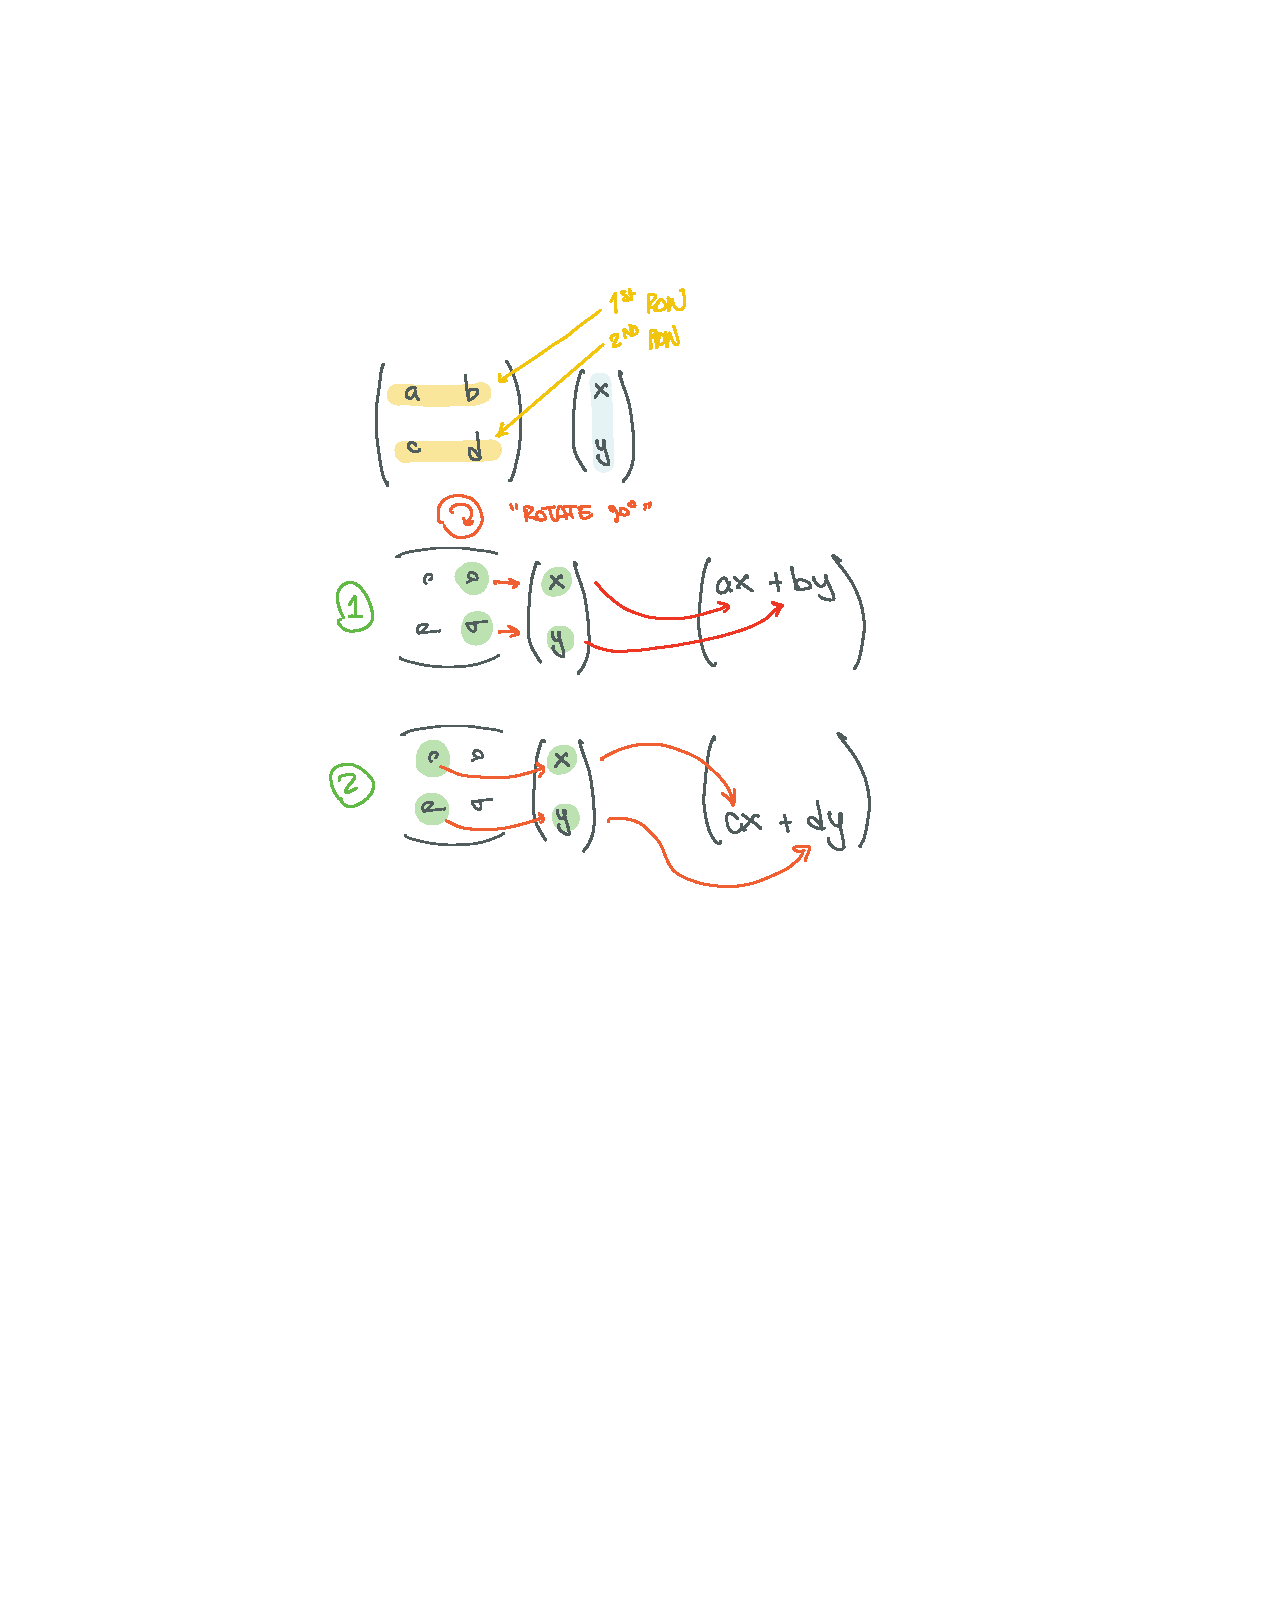
\includegraphics[width=.5\textwidth]{figures/MatrixMult_2220.pdf}
% \end{figure}
\begin{marginfigure}%[th]
    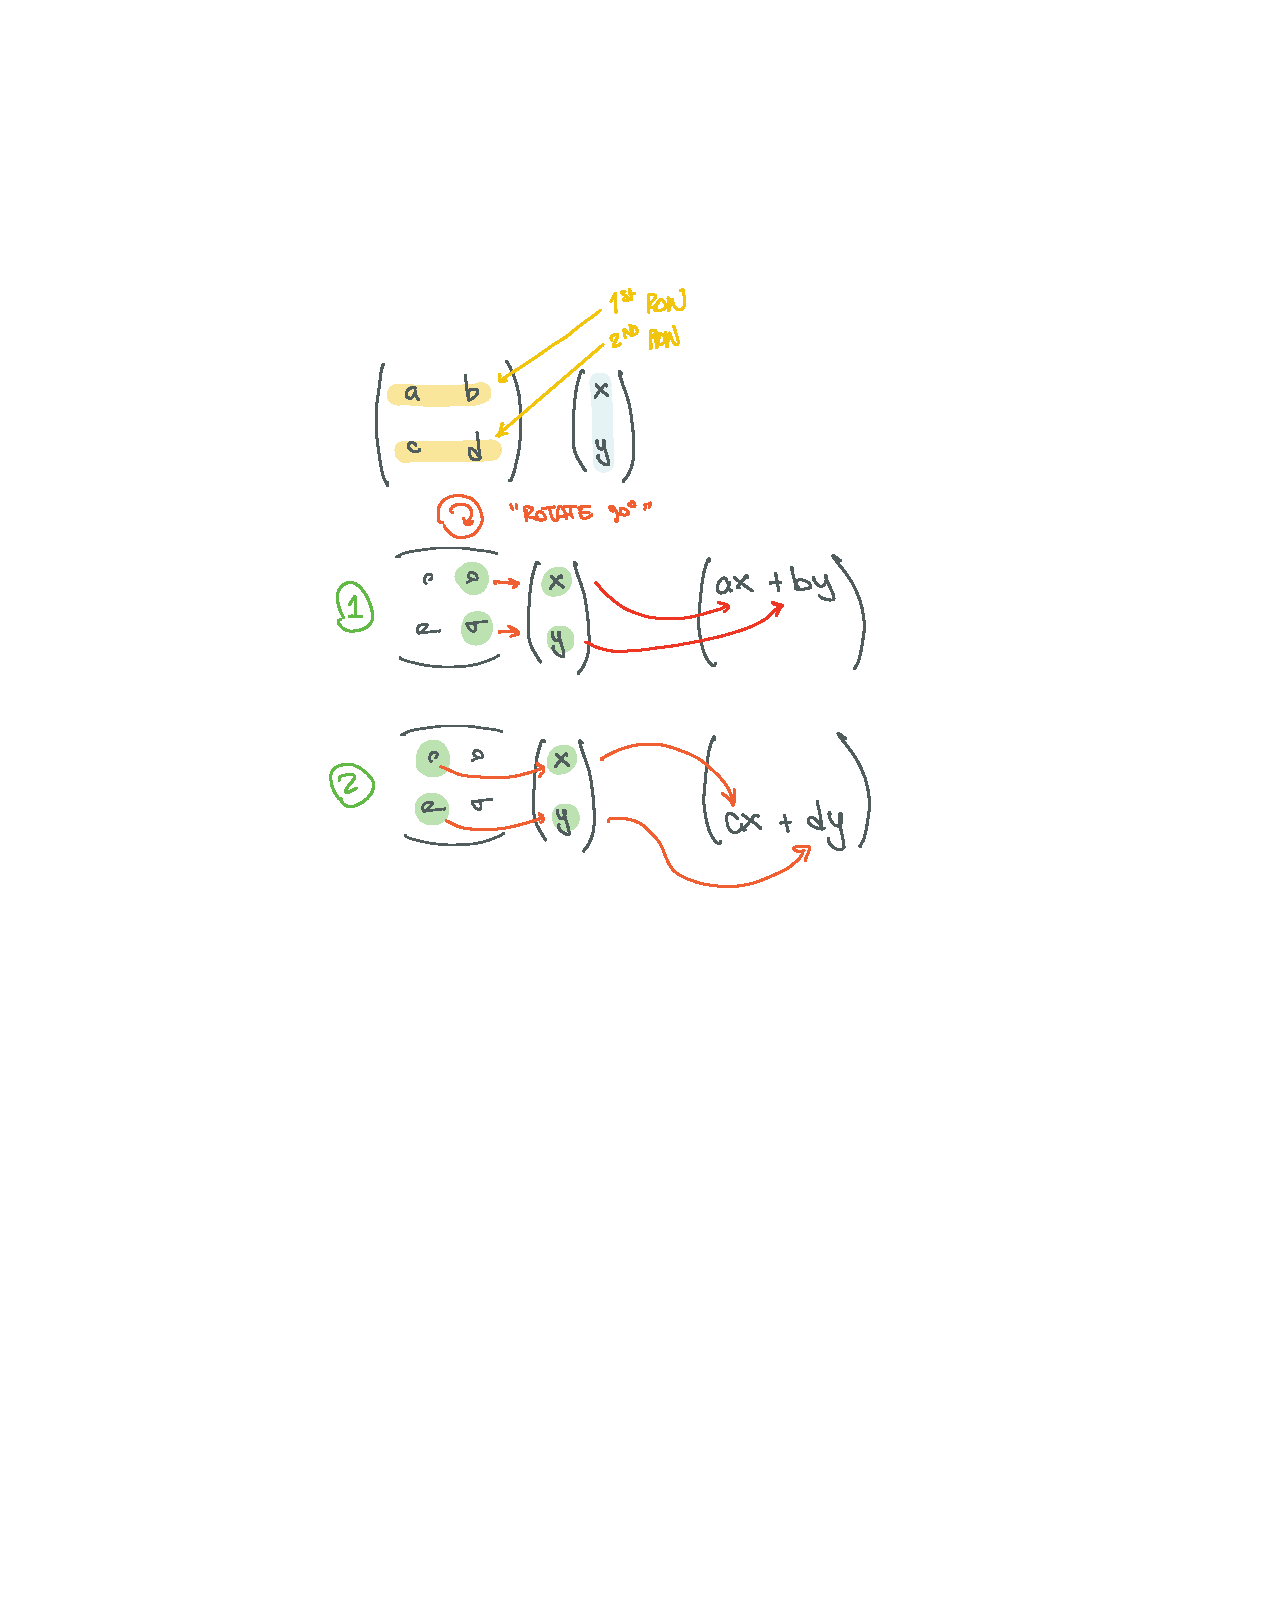
\includegraphics[width=\textwidth]{figures/MatrixMult_2220.pdf}
    \captionsetup{font={scriptsize,sf}}
    \caption{Multiplying a vector by a matrix.}
    \label{fig:matrix:mult:2220}
\end{marginfigure}
It is clunky to say the rule in words, but it goes something like this: 
\begin{enumerate}
    \item The components in the \emph{first} row of the matrix combine with the components of the column of the vector to give the \emph{first} component of $M\vec{v}$. To enact this visually,  highlight the \emph{first} row and rotate the array of numbers in $M$ clockwise by 90 degrees. The components of $M$-tipped over that are the same height as the corresponding components of $\vec{v}$ are multiplied and each product is summed together. This sum is the \emph{first} component of $M\vec{v}$.
    \item The components in the \emph{second} row of the matrix combine with the components of the column of the vector to give the \emph{second} component of $M\vec{v}$. To enact this visually,  highlight the \emph{second} row and rotate the array of numbers in $M$ clockwise by 90 degrees. The highlighted components of $M$-tipped over that are the same height as the corresponding components of $\vec{v}$ are multiplied and each product is summed together. This sum is the \emph{second} component of $M\vec{v}$.
\end{enumerate}
If you are working with three-component vectors, then there is a third step where the word `second' is replaced by `third.' 

There are other kinds of objects called row vectors. These look like vectors but they have been tipped over counter-clockwise by 90 degrees:
\begin{align}
    \row{w} = \begin{pmatrix}
        a & b
    \end{pmatrix} \ .
\end{align}
We can use this same `tip over and multiply same-height components' visualization to multiply row vectors onto vectors. See Figure~\ref{fig:matrix:mult:0220}.
\begin{figure}[ht]
    \centering
    \captionsetup{font={scriptsize,sf}}
    \sidecaption[][-2\baselineskip]{%
        Matrix multiplication of a row vector onto a [column] vector.  
        %
        %% \label command inside the \sidecaption command
        \label{fig:matrix:mult:0220}
    }
    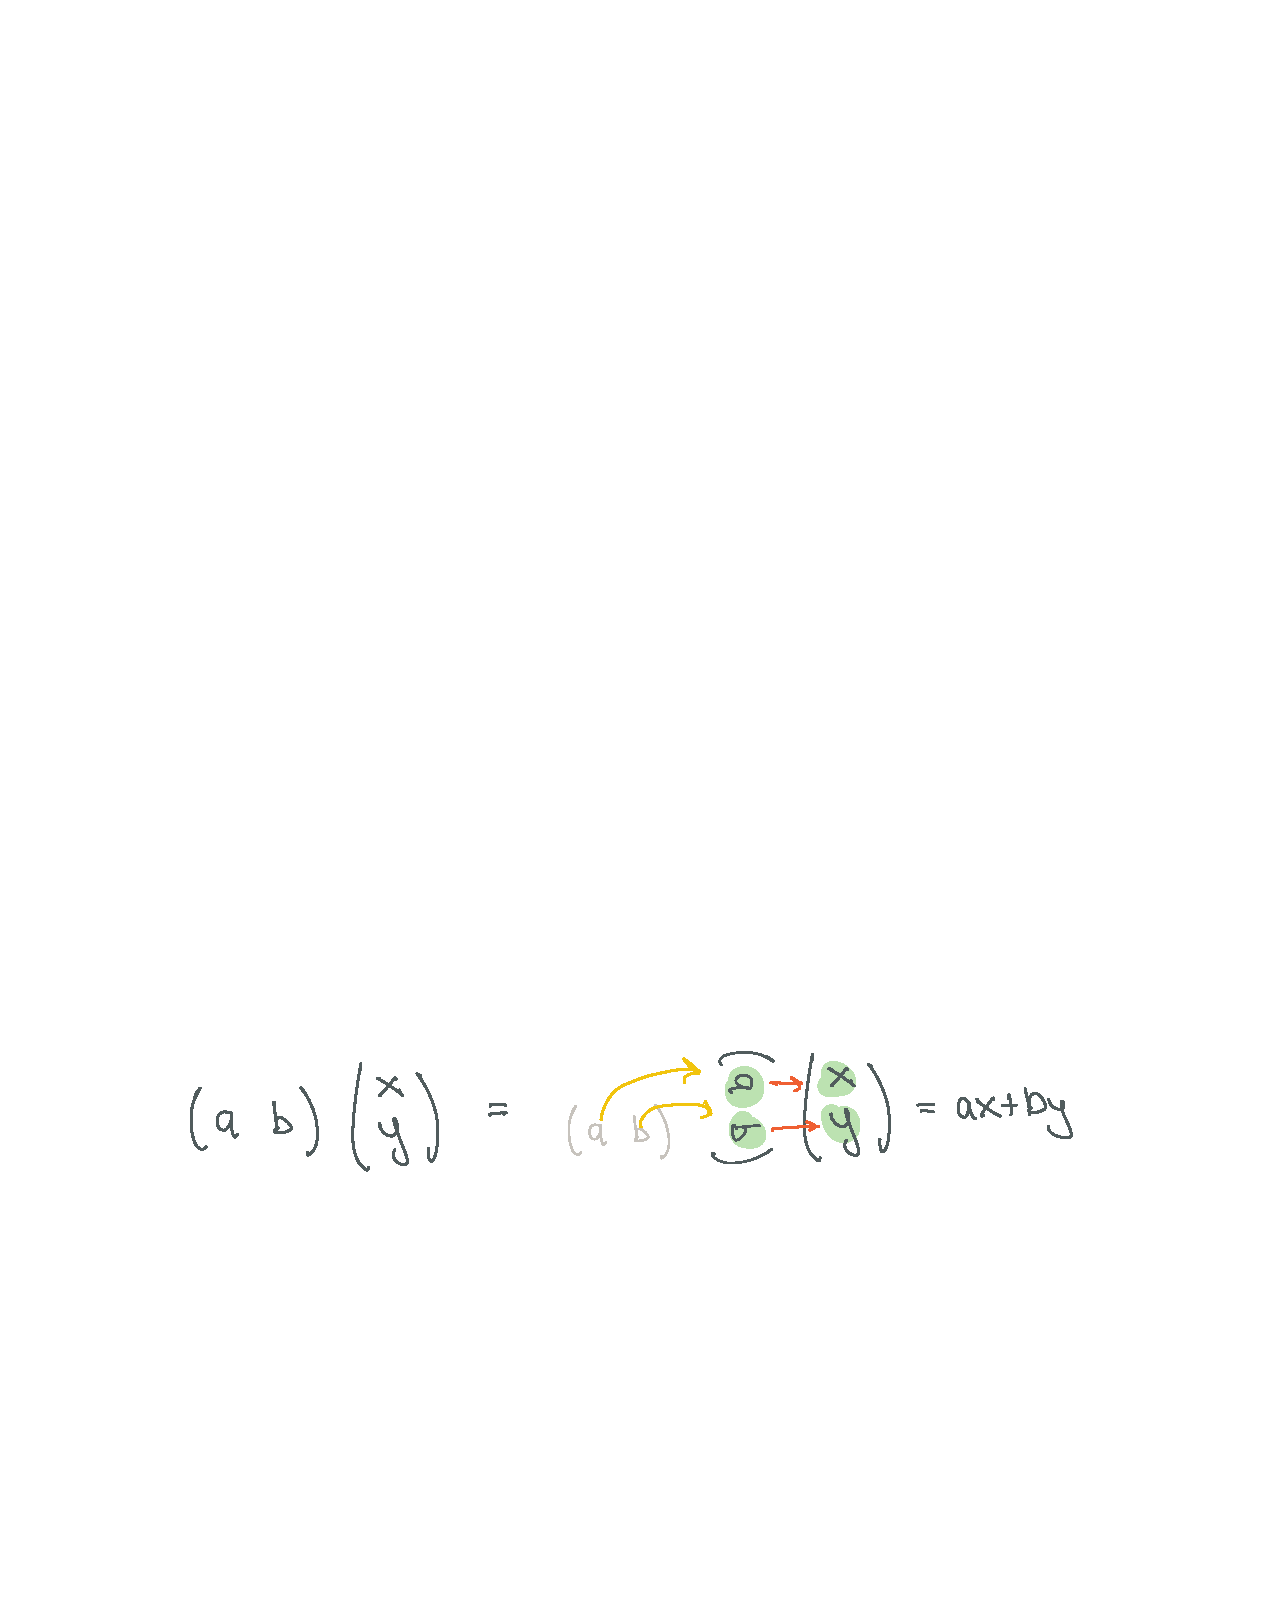
\includegraphics[width=.8\textwidth]{figures/MatrixMult_0220.pdf}
\end{figure}
Observe that the result of this multiplication is a number.
\begin{exercise}
Draw the vector
\begin{align}
    \vec{v} = \begin{pmatrix}
        1 \\ 1
    \end{pmatrix} \ .
\end{align}
Draw the vector
\begin{align}
    \begin{pmatrix}
        2 & 1 \\
        1 & 1
    \end{pmatrix}
    \begin{pmatrix}
        1 \\ 1
    \end{pmatrix} \ .
\end{align}
\end{exercise}

We can also multiply matrices with one another. The result of this is another matrix. One can construct the components of this matrix by thinking of the left matrix acting on each column of the right matrix to give the corresponding column of the matrix product. Here's how one would find the top-left component of the product of two $2\times 2$ matrices:
\begin{figure}[ht]
    \centering
    \captionsetup{font={scriptsize,sf}}
    \sidecaption[][-2\baselineskip]{%
        Multiplication of two matrices, highlighting the steps to find the top-left component of the product matrix.
        %
        %% \label command inside the \sidecaption command
        \label{fig:matrix:mult:2222a}
    }
    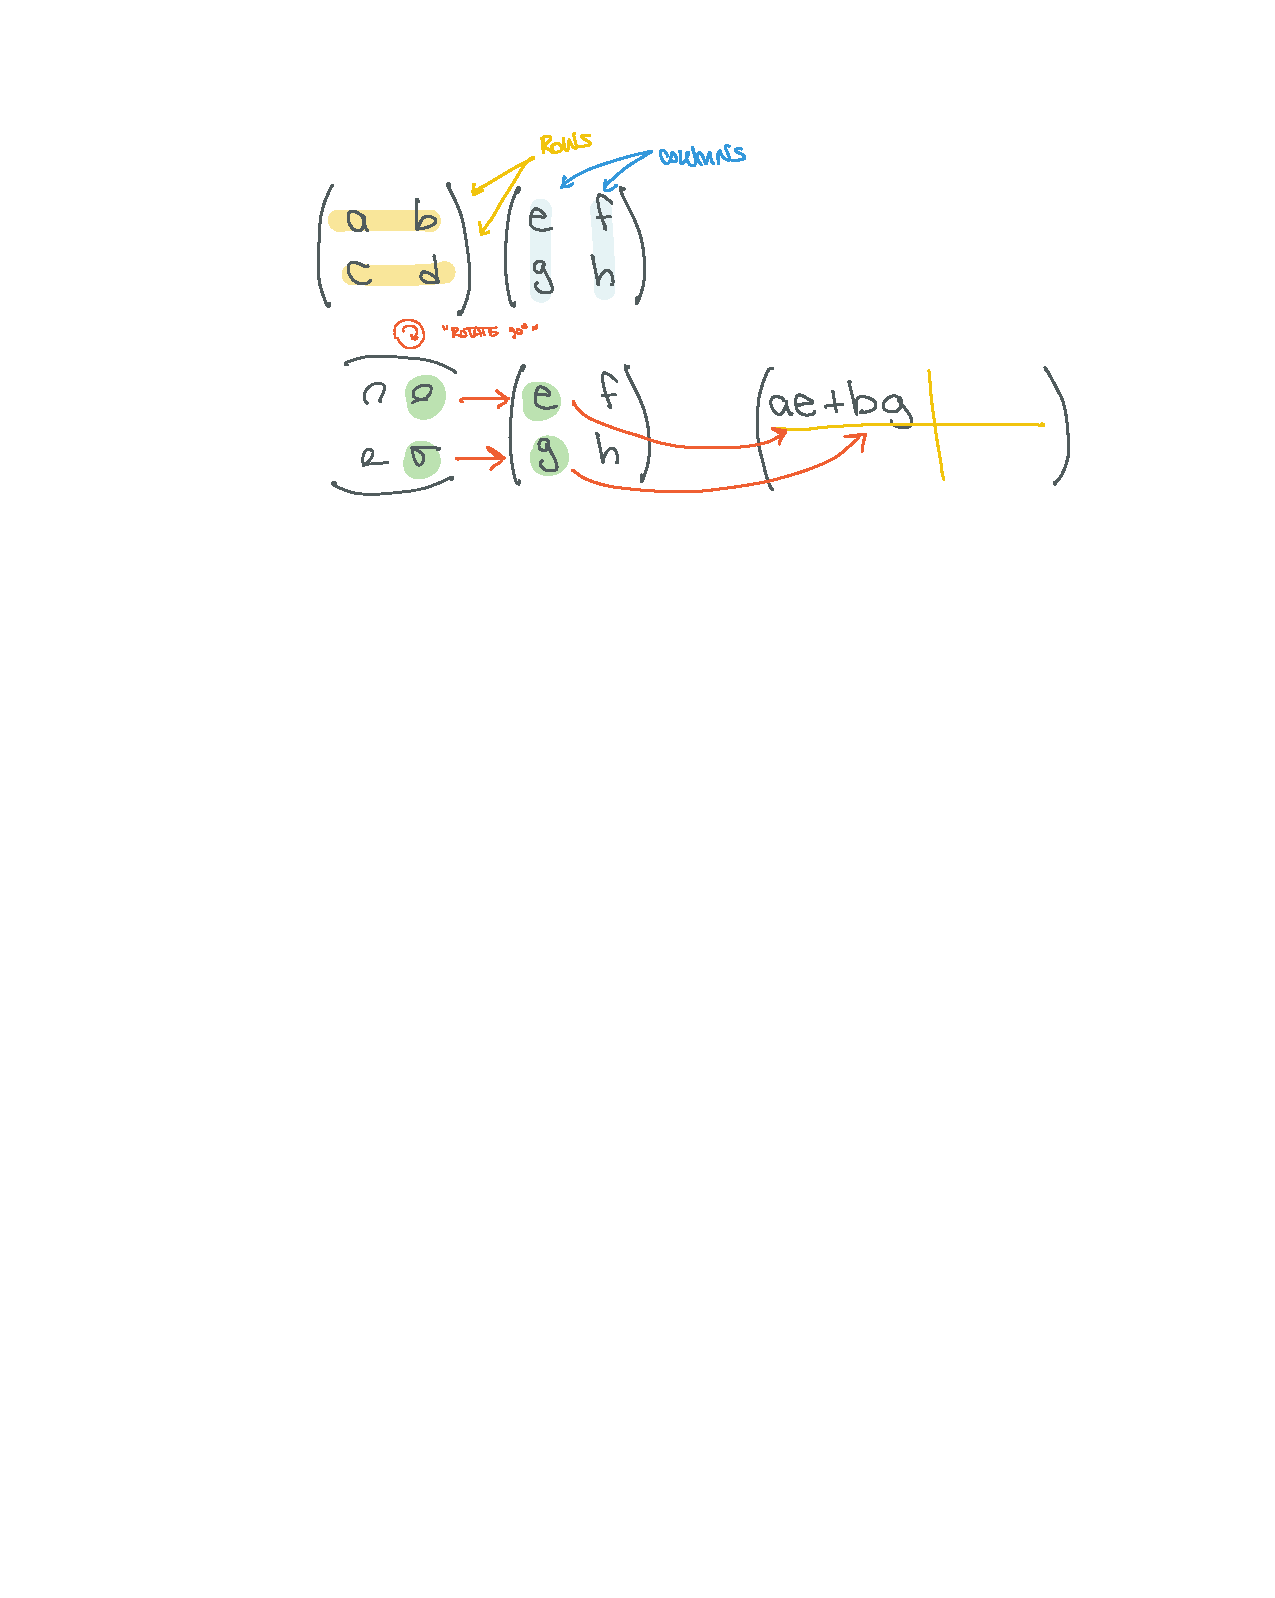
\includegraphics[width=.8\textwidth]{figures/MatrixMult_2222a.pdf}
\end{figure}
We can go on and find the top right (first row, second column) and bottom left (second row, first column) components of the product matrix, see Figure~\ref{fig:matrix:mult:2222b}.
\begin{figure}[ht]
    \centering
    \captionsetup{font={scriptsize,sf}}
    \sidecaption[][-2\baselineskip]{%
        Multiplication of two matrices, highlighting the steps to find the top right and bottom left components of the product matrix.
        %
        %% \label command inside the \sidecaption command
        \label{fig:matrix:mult:2222b}
    }
    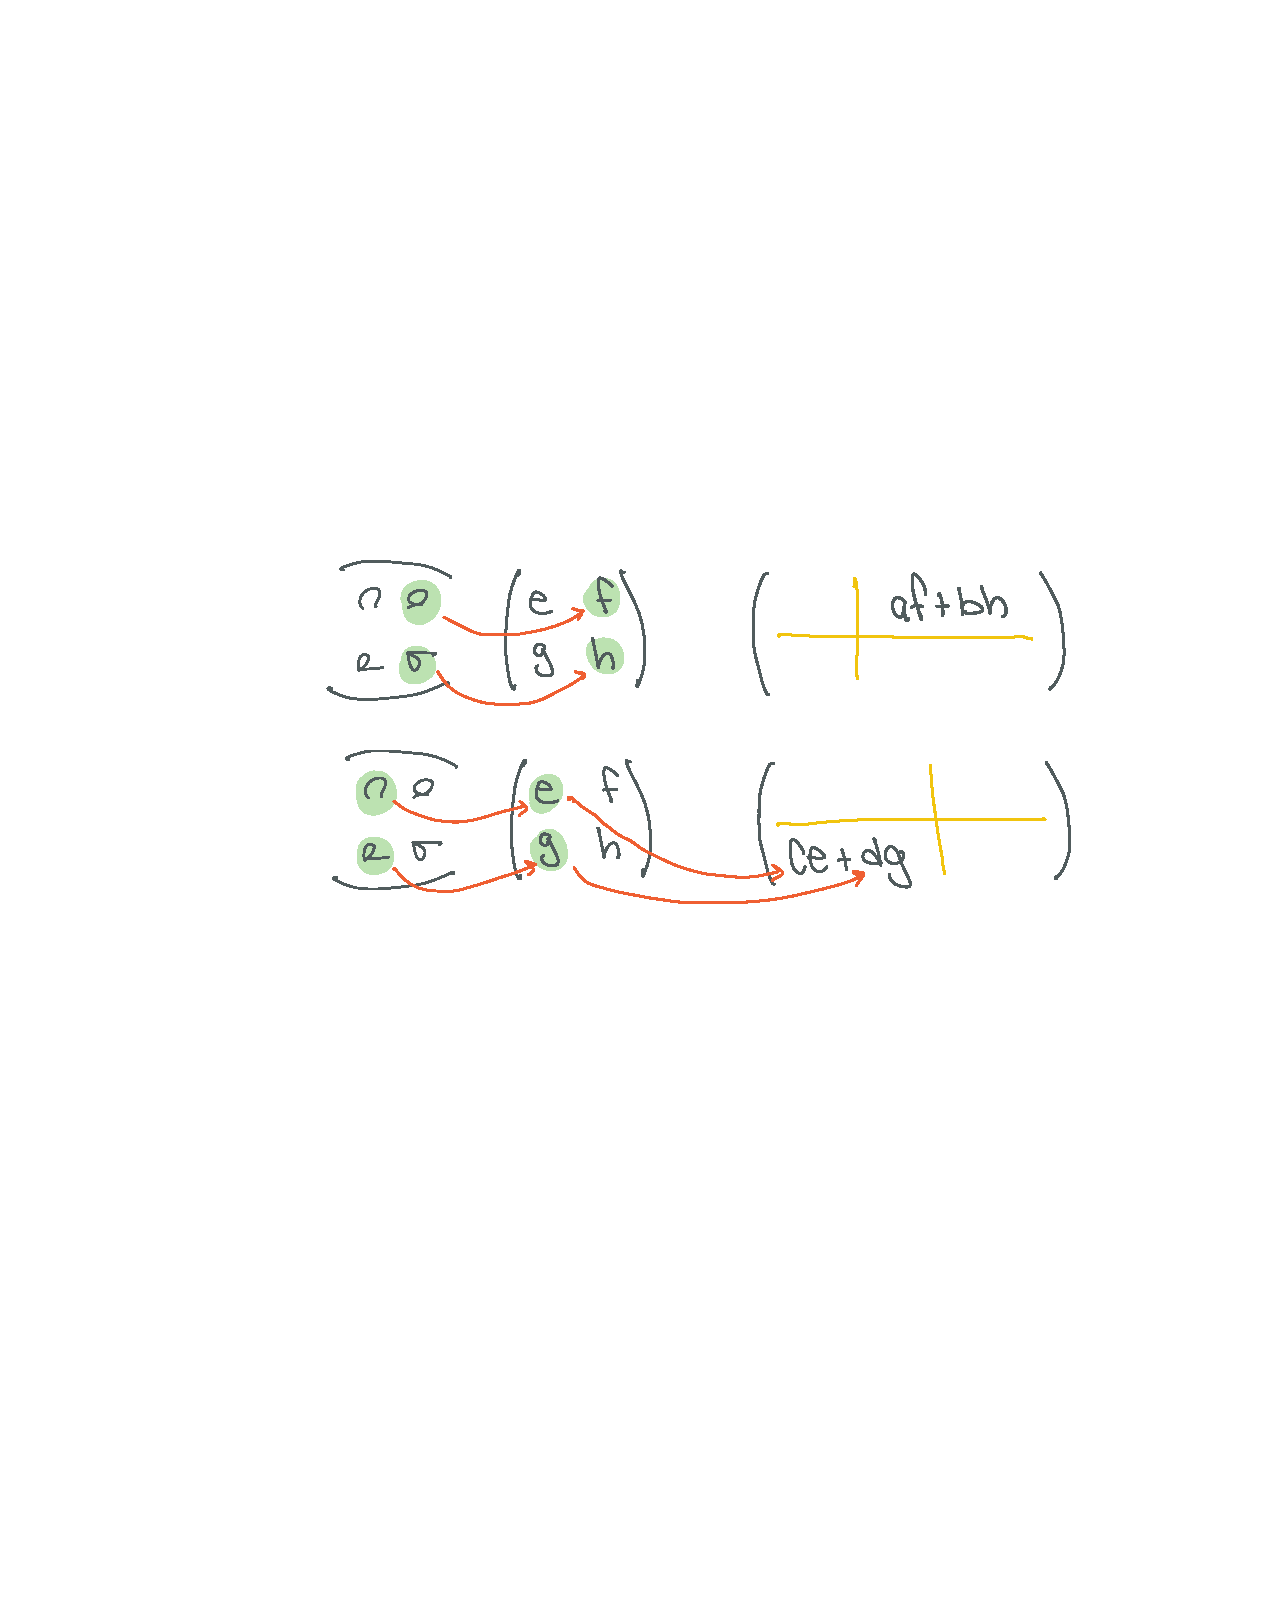
\includegraphics[width=.8\textwidth]{figures/MatrixMult_2222b.pdf}
\end{figure}
\begin{exercise}
Show that the product of two $2\times 2$ matrices $MN$ is different from the product in the opposite order, $NM$. We say that matrix multiplication is not commutative.  
\end{exercise}
\begin{exercise}
Show that
\begin{align}
\begin{pmatrix}
    2 & 1 \\
    1 & 1 
\end{pmatrix}
\begin{pmatrix}
    1 & -1 \\
    -1 & 2 
\end{pmatrix}
=
\begin{pmatrix}
    1 & 0 \\
    0 & 1
\end{pmatrix} \ .
\end{align}
The matrix on the right-hand side is called the \textbf{identity matrix}, $\one$, because when it acts on a vector it leaves the vector unchanged. We say that the two matrices on the left-hand side are \textbf{inverses}. Show further that if two matrices are inverses, $M$ and $M\inv$, then the order of the multiplication does not matter: $MM\inv M\inv M = \one$.
\end{exercise}

One can further generalize this to non-square matrices---that is, matrices with a different number of rows than columns. Those matrices will not be of direct use in this course. However, the rules of matrix multiplication follow.
\begin{exercise}
Show that you can use the matrix multiplication rules multiply a $2\times 3$ matrix onto a $3\times 2$ matrix, where our notation is $(\textnormal{number of rows})\times(\textnormal{number of columns})$.
\end{exercise}
\begin{exercise}
Show that you \emph{cannot} multiply a $2\times 3$ matrix onto a $2 \times 3$ matrix. 
\end{exercise}
\begin{exercise}
Suppose you want to multiply an $n\times m$ matrix onto a $k \times \ell$ matrix.. What are the conditions on the numbers $n, m, k, \ell$ for this to make sense using the matrix multiplication rule?
\end{exercise}



The rules for matrix multiplication also introduces the notion of a matrix inverse. Given a matrix $M$, the inverse of the matrix $M\inv$ `undoes' whatever the matrix does. It is also true that $M$ `undoes' whatever $M\inv$ does. In this sense $(M\inv)\inv = M$. The defining relation is
\begin{align}
    M M\inv = M\inv M = \one \ ,
    \label{eq:matrix:invers:multiplcation:notation}
\end{align}
where $\one$ is the identity matrix that is zero except for ones along the diagonal.\sidenote{When $\one$ acts on a vector it returns the same vector: $\one \vec{v} = \vec{v}$.}
\begin{exercise}\label{ex:matrix:inversino:the:hard:way}
Let us assign values to $M$ and $M\inv$ in the $2\times 2$ case:
\begin{align}
M &=
    \begin{pmatrix}
    a & b \\
    c & d    
    \end{pmatrix}
    &
M\inv &=
    \begin{pmatrix}
    x & y \\
    z & w    
    \end{pmatrix} \ .
\end{align}
Write out the \emph{four} conditions that we get from $MM\inv = \one$. \textsc{Partial answer}: one of the conditions is
\begin{align}
    ax + bz = 1 \ .
\end{align}
If you know each of the components of $M$, then you have four equations for four unknowns. This system of equations may have a solution.
\end{exercise}
\begin{exercise}
Using the system of equations above, prove the usual identity for $2\times 2$ invertible matrices:
\begin{align}
    M\inv = \frac{1}{ad-bc}
    \begin{pmatrix}
    \pp d & -b \\
    -c & \pp a    
    \end{pmatrix} \ .
\end{align}
\end{exercise}
All of this assumes that the inverse is well defined, which is not always the case. For example, if either a row or a column of $M$ is all zeros---the matrix will not be invertible. This is because the matrix \emph{projects out} information and there is no way to recover that information.



This notion of matrix multiplication is helpful and perhaps something you may have learned in earlier stages of your education. It is still the way I do many calculations. \emph{However}, the rules in this section are a \emph{shortcut} for a much richer mathematical structure. It is this mathematical structure that we want to reveal because it shows us how seemingly different mathematical structures in physics are actually rooted in the same underlying language. As such, many of the notions in this chapter may be ideas that you must first \emph{unlearn} in order to \emph{relearn} how they are outputs of the richer structure.\sidenote{When I teach this class there are often a few students who are apologetic for not having taken a formal linear algebra class. I have noticed that those students sometimes do much better in the course because they have fewer preconceptions to unlearn.}


\section{Rotations}\label{sec:Euclidean:three:space:rotations}

Rotations are transformations that take vectors into other vectors. They are a specific example of what is more generally known as an \emph{isometry}---and idea that we shall refer to over and over in this course. Your intuition about rotations may align with the following observations:
\begin{itemize}
    \item Rotations preserve the magnitude of vectors.
    \item Rotations preserve the angle between vectors. 
\end{itemize}
Because both magnitude and angle are related to the dot product, you may guess that rotations have something to do with the dot product. This is correct---but we need to build up some mathematical structure before we can articulate this idea carefully. In this section, we simply whet your appetite by saying that a `working definition' of rotations in Euclidean space of any dimension is that a rotation is a matrix $R$ that satisfies
\begin{align}
    R^\trans R = \one \ ,
    \label{eq:RTR:one}
\end{align}
where the \textbf{transpose} of a matrix $R^\trans$ is what happens when you flip all the elements along the diagonal:
\begin{align}
    \begin{pmatrix}
        a & b \\
        c & d
    \end{pmatrix}^\trans \defeq
    \begin{pmatrix}
        a & c \\
        b & d
    \end{pmatrix} \ .
\end{align}
We write $\one$ to mean the unit matrix: the matrix with only ones along the diagonal. Matrices $R$ that satisfy \eqref{eq:RTR:one} are called \textbf{orthogonal}\index{orthogonal}---this is just a fancy name for rotation. 

\begin{exercise}
Show that the standard form of a rotation in two dimensions,
\begin{align}
R=
    \begin{pmatrix}
    \cos \theta & -\sin\theta \\
    \sin \theta & \cos\theta      
    \end{pmatrix} \ .
\end{align}
satisfies \eqref{eq:RTR:one}. Using this form of rotations, show that rotations in 2-dimensional Euclidean space preserve the length of vectors and the angle between vectors. \textsc{Hint}: use $\cos^2\theta + \sin^2\theta = 1$.
\end{exercise}





\chapter{Indexology}\label{ch:indexology}
\begin{quote}
... should not prevent us from avoiding purely formal calculations where a \emph{debauchery of indices} hides an often simple geometrical reality. -- E.~Cartan, \emph{Lecons sur la Geometrie des Espaces de Riemann}\sidenote{From Spivak, \emph{A Comprehensive Introduction to Differential Geometry}, volume 2.}\footnote{\cite{spivak1975comprehensive}; see also \url{spivak1975comprehensive}}
\end{quote} % cite https://hsm.stackexchange.com/questions/3320/the-debauch-of-indices-translation-request

In this chapter we introduce the rules for index notation. Please accept them for now as a necessary complication---there is nothing deep here, only a set of conventions and one useful shorthand (summation convention). The utility of these may not be obvious until we start to see how this is used and where it comes from.

\section{Tensors and index notation}
\label{sec:index:notation}

In this course we make a \emph{big deal} about the height of indices. This means the index does more than  `index' a number in an array. In fact, in physics there are objects that carry multiple indices with different heights. Here is one such example, the Riemann tensor in general relativity: $R^a_{\phantom{a}bcd}$. This object has four indices. The first one, $^a$ is raised, and the following three, $_{bcd}$ are lowered. There needs to be an unambiguous ordering of the indices: it is clear that the index $b$ is the \emph{second} index, the index $c$ is the \emph{third} index, and so forth. So it would be disastrous to write $R^a_{bcd}$ because now we cannot tell whether the upper index $^a$ or the lower index $_b$ is the \emph{first} index. This is demonstrated in Figure~\ref{fig:Riemann:tensor:for:indices}.
\begin{marginfigure}%[th]
    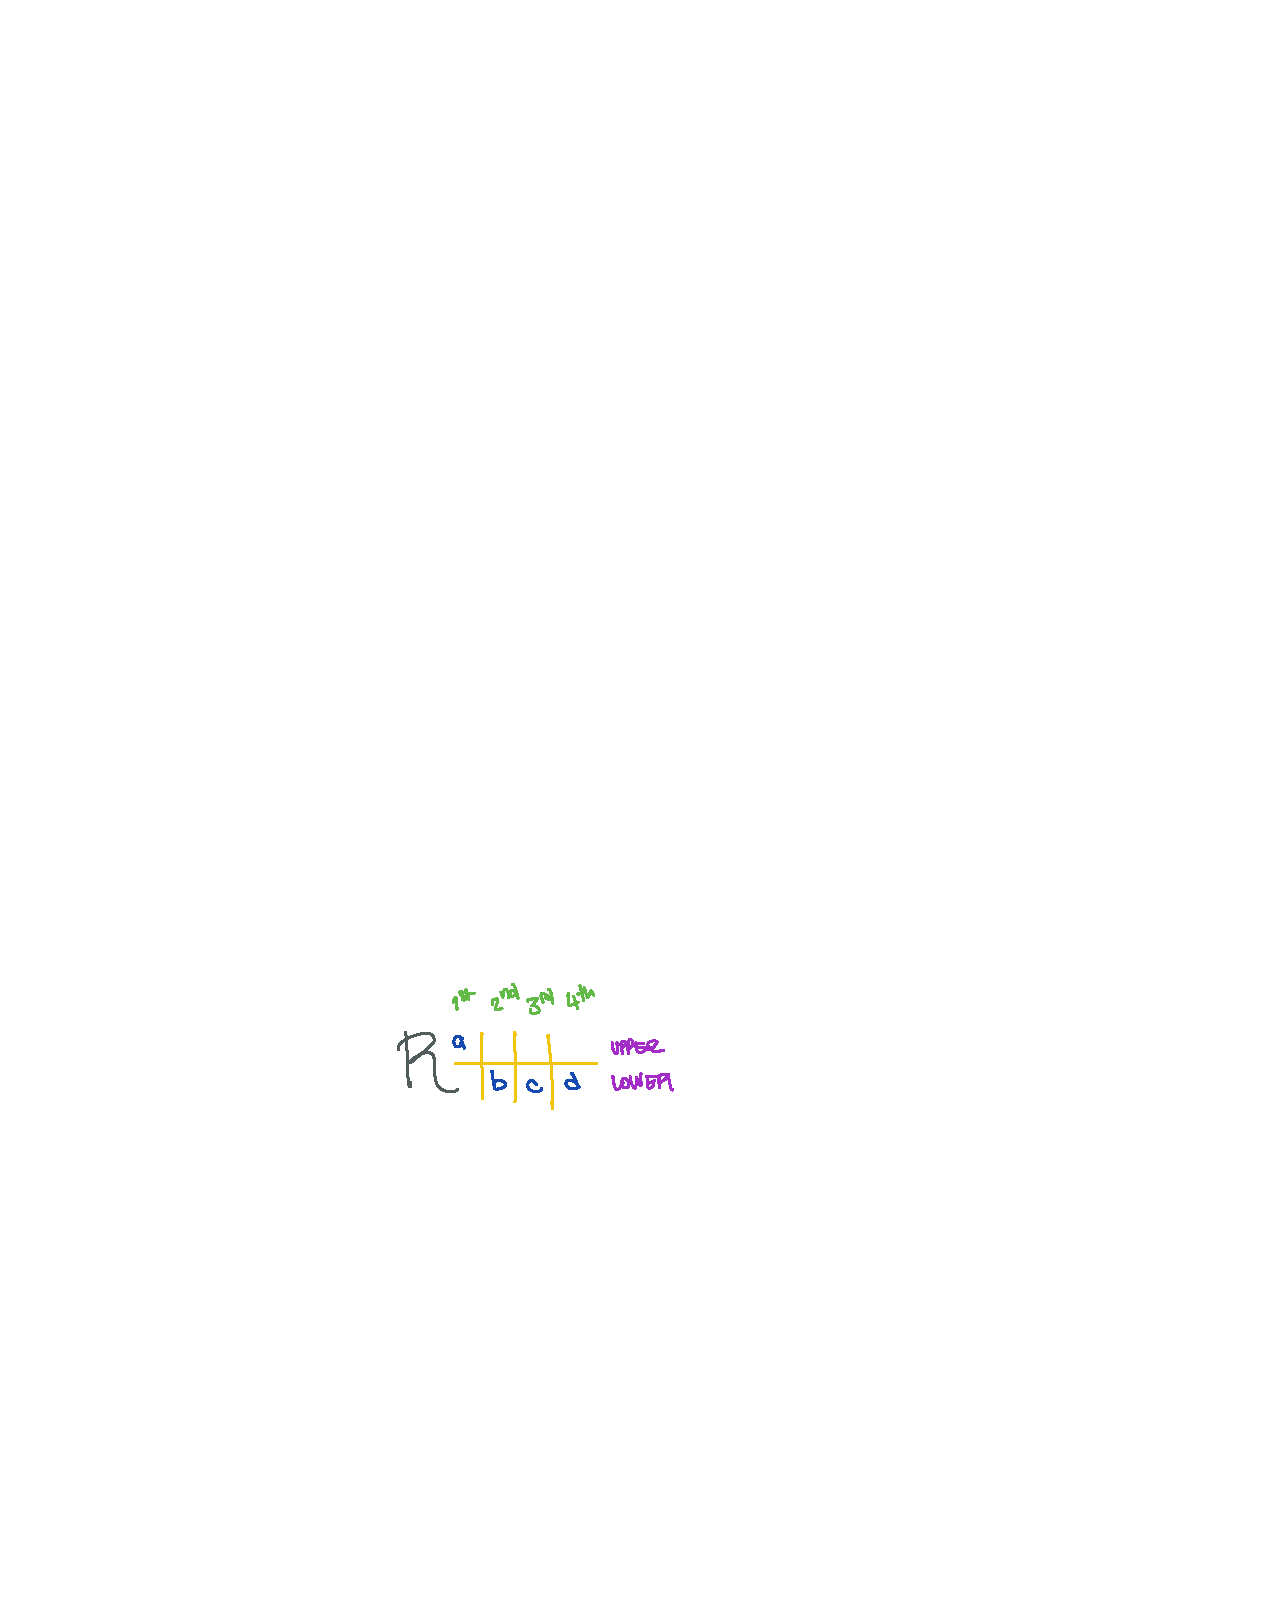
\includegraphics[width=.8\textwidth]{figures/Rabcd_eg.pdf}
    \captionsetup{font={scriptsize,sf}}
    \caption{The Riemann tensor showing the significance of the ordering and height of its indices.}
    \label{fig:Riemann:tensor:for:indices}
\end{marginfigure}

So let us get to the elephant in the room. To a physicist, a \textbf{tensor}\index{tensor} is an object that has indices. In this sense, vectors and matrices are both types of tensors. They can have any number of indices, but the indices have a well defined order and a well defined height (raised or lowered). In general, the following two objects are different:
\begin{align}
    M\aij{i}{j} &&\text{and} && M_i^{\phantom{i}j} \,
\end{align}
even though both are two-index objects whose first index is $i$ and second index is $j$. 

Why do we make such a big deal about indices and their heights? The difference between a tensor and an array of numbers is that tensors have specific \emph{transformation rules} under symmetries. The symmetry that you are most familiar with is rotational symmetry. From your first-year coursework, you are familiar with how useful it is to rotate to coordinates where a problem is simpler. The most common example of this is calculating the moment of inertia of a rotating body. There we had an object called the \emph{moment of inertia tensor}\sidenote{The transformation rules of this tensor are precisely why it is not called a ``moment of inertia \emph{matrix}.'' Though you may be hard pressed to find an honest textbook that explains this.\footnotemark}\footnotetext{See e.g.\,\url{https://hepweb.ucsd.edu/ph110b/110b_notes/node24.html}} One of the groan-inducing exercises in mechanics is to find the rotation in which the moment of inertia tensor of a rotating body is diagonal.

Here is what we need to know for now:
\begin{enumerate}
    \item In physics, tensors are objects with indices. These are arrays of numbers so that a particular choice of indices corresponds to a number in the tensor. The order of the indices matters.
    \item But there is more: whether an index is upper or lower indicates how that part of the tensor transforms under a symmetry transformation such a rotations. 
\end{enumerate}
At this point, you may have several questions, such as these:
\begin{enumerate}
    \item How exactly does a tensor transform under symmetries?
    \item What are examples of other symmetries?
    \item How should I visualize an object with more than two indices? (Yes, you can think of a three-index object as a hypercube arrays of numbers. No, I do not know of a good way to visualize upper versus lower indices on this array.)
\end{enumerate}
We shall answer these as we build up the machinery below. Just take this section as a request to believe that there may be method to this madness.

\section{The treachery of indices}
\label{sec:treachery:of:indices:vi:is:not:a:vector}

There is something that physicists do that tend to drive mathematicians crazy: we write a generic \emph{component of a vector} and refer to it as if it were the vector itself. It is a fairly harmless peccadillo:\sidenote{There are times when you can get into trouble if you drink your own Kool Aid, so to speak. The reason is that the \emph{component} $v^i$ is simply a number, whereas $\vec{v}$ is a vector. Some manipulations are only allowed for numbers and not vectors, and you should be clear that you mean `the component $v^i$' if you are treating it like a number, and not `the \emph{vector} whose components are $v^i$.' %See Example~\ref{eg:moving:coefficients:around}.
} if I say
\begin{quote}
the vector $v^i$
\end{quote}
then it is not hard to guess that I mean
\begin{quote}
the vector $\vec{v}$ which has components that I label $v^i$.
\end{quote}
If you ever meet a mathematician who gives you a hard time about this, you can wave your hands and refer to something called \emph{abstract index notation}, developed by Roger Penrose.\footnote{\url{https://math.stackexchange.com/questions/455478/}} To the best of my understanding, this is simply a formal way to justify the way physicists talk about indices. 

The reason why we have this culture is that this index notation ends up being so damn convenient. In addition to vectors, we will have other objects that have indices: dual vectors, matrices, and tensors. When we write everything in with indices, we can ``see'' properties of these objects that are not obvious without the indices. Specifically, we can see \emph{how an object transforms under symmetries}. In this course, we will focus on \emph{rotations} of vectors and their generalizations. 

Whenever I think about whether $v^i$ means the vector $\vec{v}$ or the $i^\textnormal{th}$ component of that vector, I am reminded of Magritte's ``The Treachery of Images,'' Figure~\ref{fig:Magritte}\footnote{From \url{https://en.wikipedia.org/wiki/The_Treachery_of_Images}, please refer to this page for fair use justification.}
\begin{marginfigure}%[th]
    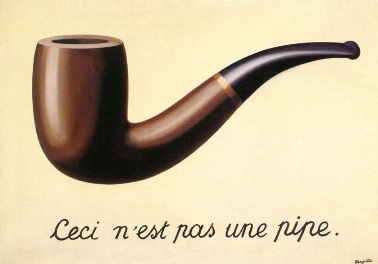
\includegraphics[width=.8\textwidth]{figures/MagrittePipe.jpg}
    \captionsetup{font={scriptsize,sf}}
    \caption{``La Trahison des Images'' (``The Treachery of Images'') by Ren\'e Magritte. Owned by \tacro{LACMA}, reproduced here under fair use.}
    \label{fig:Magritte}
\end{marginfigure}
In this image, Magritte shows a painting of a pipe and then writes ``this is not a pipe.'' The implied message is that it is a \emph{painting} of a pipe that we may use to express the \emph{idea} of a pipe.


\section{Summation Convention}
\label{sec:summation}


There is another reason why indices are convenient: they allow us to use \textbf{summation convention}.\sidenote{Sometimes called Einstein summation convention in deference to its progenitor. With respect to Einstein, we simply write \emph{summation convention} because it's not like the dude is underappreciated in popular culture.} This is a notational shortcut that introduces upper and lower indices to convey sums. Consider, for example, the ``matrix multiplication'' of a row vector $\row{w}$ on a column vector $\vec{v}$. Nevermind the formal definition of ``row vector'' as opposed to ``column vector.'' Let us write it out in components where it is obvious for $\RR ^3$:
\begin{wide}
\begin{align}
    \row{w}
    &=
    \begin{pmatrix}
        w_1 & w_2 & w_3
    \end{pmatrix}
    &
    \vec{v}
    &=
    \begin{pmatrix}
        v^1 \\ v^2 \\ v^3
    \end{pmatrix}
    &
    \row{w}\vec{v}
    &= w_1v^1 + w_2v^2+w_3v^3 \ .
\end{align}
\end{wide}
On the far right we have used the matrix multiplication rules in Section~\ref{sec:matrix:multiplication}.
% The final expression is familiar, right? It follows the usual rules of matrix multiplication for a ``matrix'' that happens to be one row and three columns; 
We review this rule in Fig.~\ref{fig:row:col:mult}, labeling the components with upper and lower indices as appropriate.
% %% FIGURE SNIPPIT
\begin{marginfigure}[.01em]%[tb]
    \centering
    \captionsetup{font={scriptsize,sf}}
    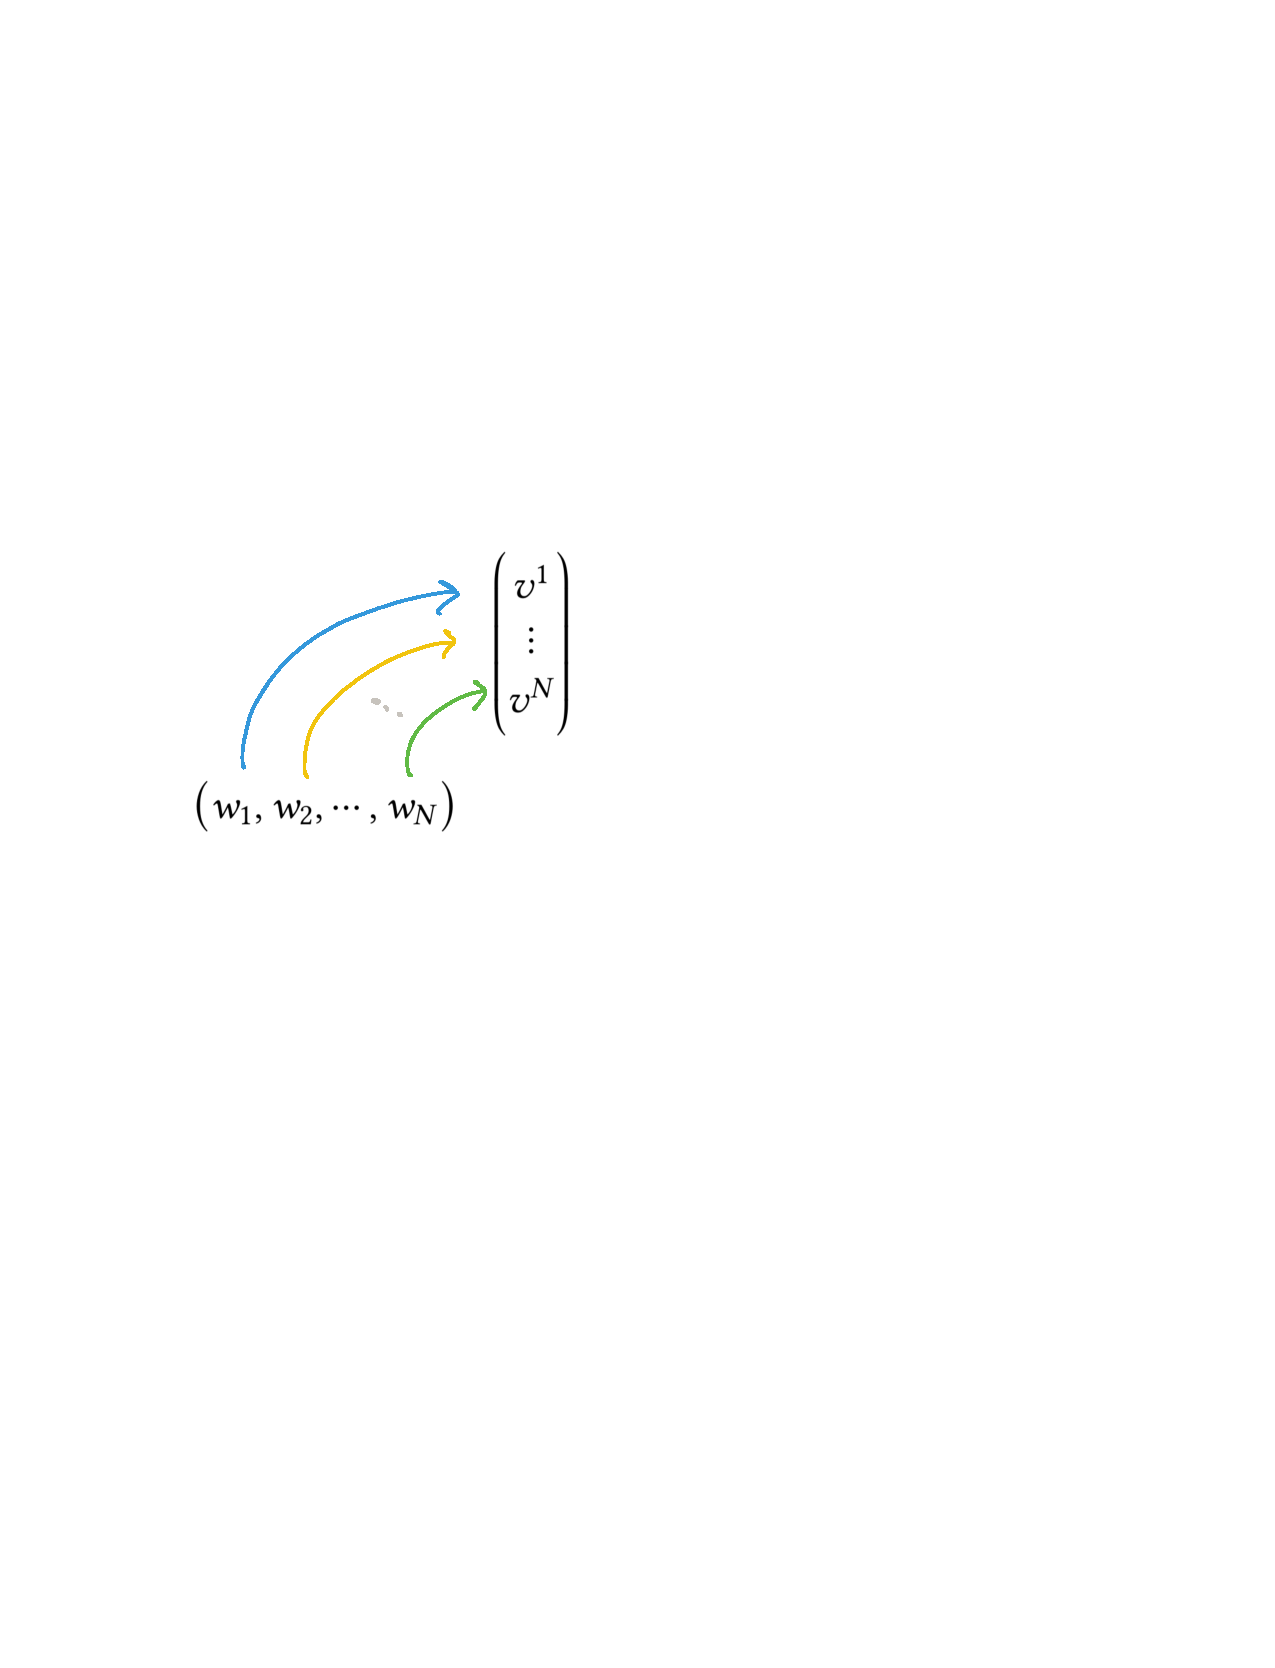
\includegraphics[width=.8\textwidth]{figures/rowcolmult.pdf}
    \caption{The `matrix multiplication rule' for acting with a row vector on a column vector.}
    \label{fig:row:col:mult}
\end{marginfigure}
Notice that we choose to write the components of $\row{w}$ with lower indices---this is the convention. Row vectors have indices written as subscripts while column vectors have indices written as superscripts. There is no mathematics here, just a choice of notation. The result of the multiplication is simply a number, which we can write as a sum:
\begin{align}
    \row{w}\vec{v}
    &= \sum_{i=1}^3 w_iv^i
    \equiv w_iv^i \ .
    \label{eq:row:w:on:vec:v}
\end{align}
On the right-hand side we have \emph{defined} the summation convention:
\begin{newrule}[Summation convention]
Whenever there is exactly one upper index and exactly one lower index with the same letter, we should understand that there is a sum over that index over all of its allowed values. We call pairs of repeated indices where one is upper and one is lower \textbf{contracted indices}\index{contract}.
\end{newrule}



The value $w_iv^i$ is simply a number. It is not a vector. It does not have any ``vectorial'' (tensorial) structure. It is not an element of the vector space $\RR ^3$. It does not transform under rotations. It is \emph{just a number}. In other words, $w_iv^i$ behaves like an object with \emph{no indices}. Contracted indices ``cancel each other out.''

This is significant because we will see that indices tell us how objects transform. Evidently, column vectors and row vectors transform differently since one has an upper index and one has a lower index. Further, when we contract the two indices, we end up with something with no indices: a number that does not transform at all. This may seem like notational overkill---trust me, it is worth building this notation now. We will use it over and over.



\begin{example}
Matrices $M$ have the following index structure: $M\aij{i}{j}$. There is a first index and a second index---the order matters. The first index is upper, and the second index is lower. Matrix multiplication boils down to a contraction of indices:
\begin{align}
    (M\vec{v})^i = M\aij{i}{j}v^j \ .
    \label{eq:matrix:mult:ith:comp}
\end{align}
Let us read this equation carefully. First, $M\vec{v}$ is a vector. The $i^\text{th}$ component of this vector is $(M\vec{v})^i$. How is this related to the components of $M$ and $\vec{v}$? The right-hand side tells us that we simply take the sum:
\begin{align}
    M\aij{i}{j}v^j = 
    M\aij{i}{1}v^1 + M\aij{i}{2}v^2  + M\aij{i}{3}v^3 \ .
\end{align}
\end{example}

\begin{figure}[tb]
    \centering
    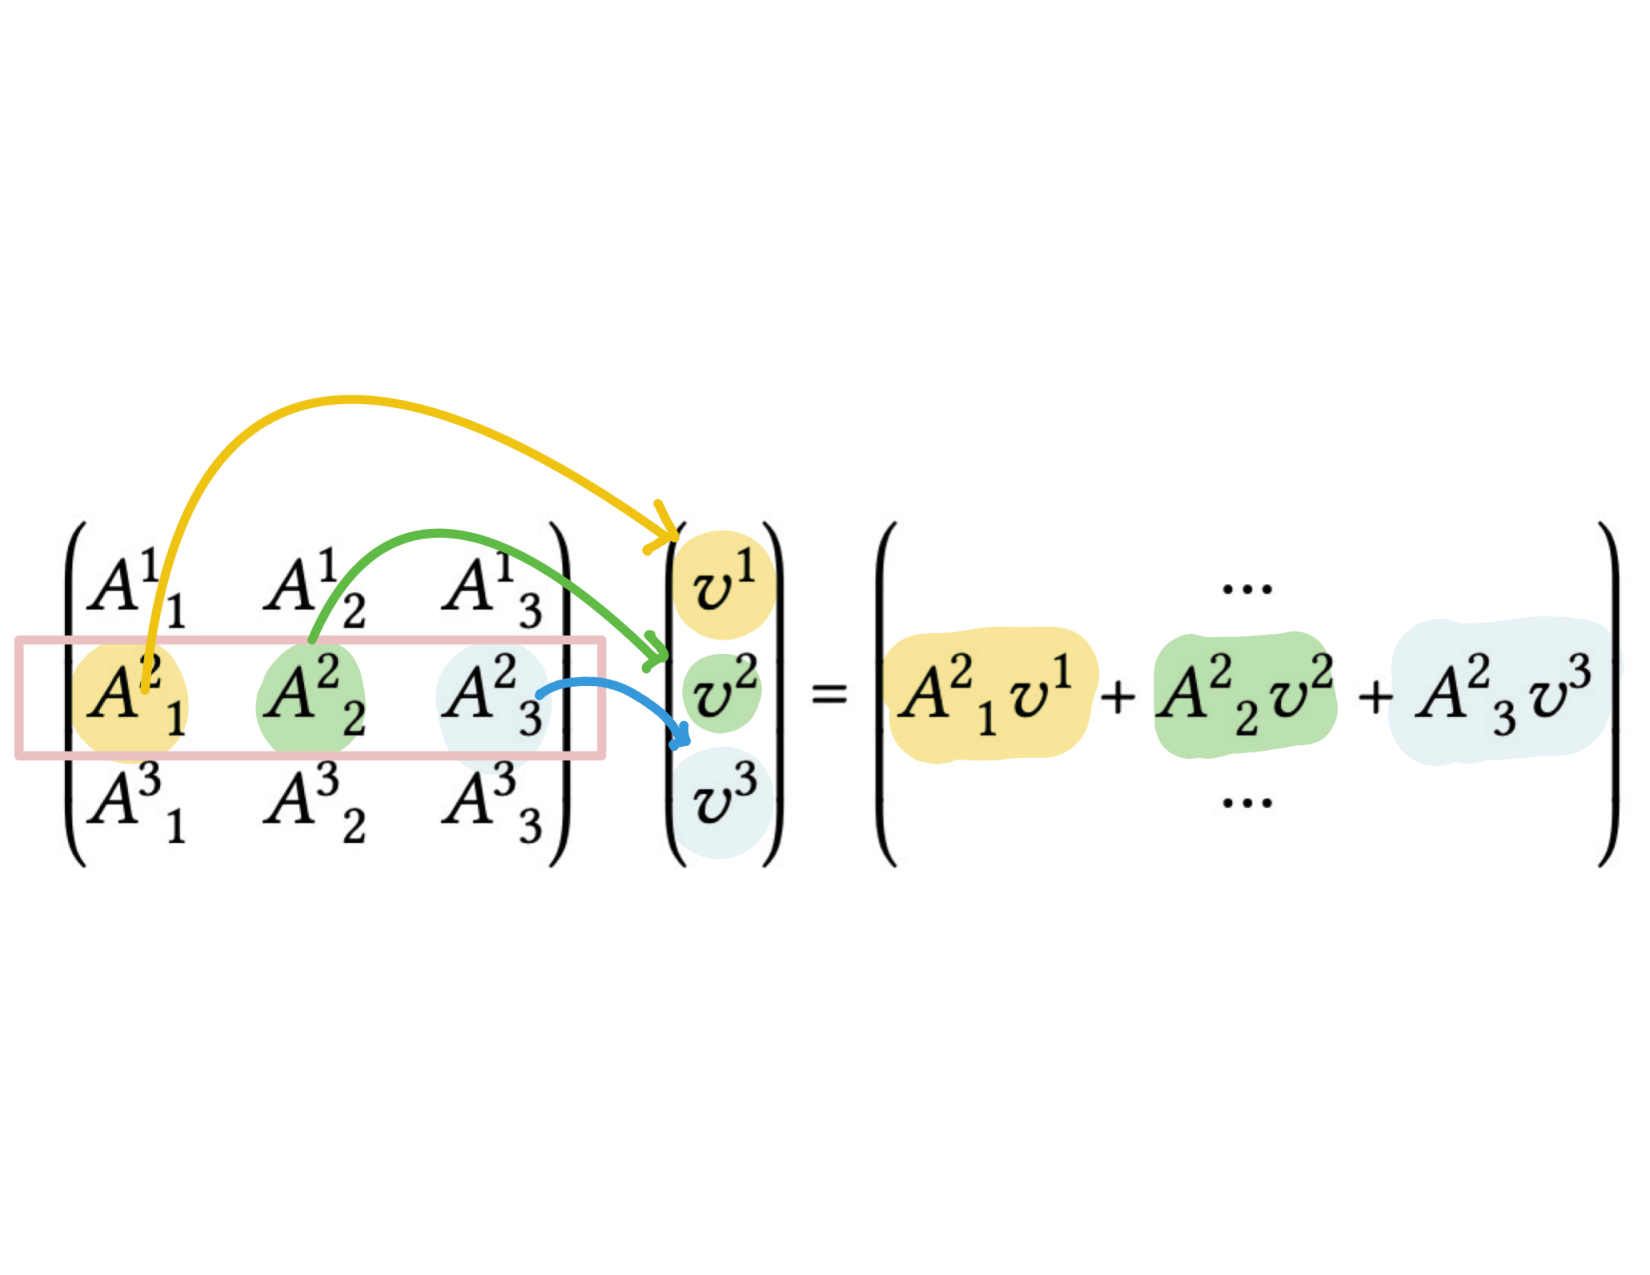
\includegraphics[width=.5\textwidth]{figures/matrixmultiplication.pdf}
    \caption{The `matrix multiplication' rule for $A\vec{v} = \vec{v}'$. We show that the second element of $\vec{v}'$ is a sum of terms, where each term is a multiplication of the $j^\text{th}$ column of the $2^\text{nd}$ row of $A$ by the $j^\text{th}$ row of $\vec{v}$.}
    \label{fig:matrix:col:mult}
\end{figure}

\begin{example}
From the above example, you can then excuse the glib statement: ``the \emph{vector} $M\aij{i}{j}v^j$.'' As we explained above, $M\aij{i}{j}v^j$ is not a vector, but a component of a vector. However, the point is that even though there are three indices, two of them are contracted so the object effectively only has one upper index. This is the index structure of a vector. This matches the usual matrix multiplication rule shown in Fig.~\ref{fig:matrix:col:mult}.
\end{example}

\begin{exercise}
Consider the following vector, row vector, and matrix:
\begin{align}
    \vec{v} &=
    \begin{pmatrix}
     1 \\ 2 \\ 3   
    \end{pmatrix}
    &
    \row{w} &=
    \begin{pmatrix}
        4&5&6
    \end{pmatrix}
    &
    M&=
    \begin{pmatrix}
        1 & 2 & 3 \\
        4 & 5 & 6 \\
        7 & 8 & 9
    \end{pmatrix} \ .
\end{align}
These have index structure $v^i$, $w_i$, and $M\aij{i}{j}$ respectively. Note that the first index of a matrix is the row and the second is the column, thus $M\aij{1}{2} = 2$ while $M\aij{2}{1} = 4$. Calculate the following: $(wM)_2$, $(Mv)^1$, $(MM)\aij{1}{2}$. Here $MM$ is understood to be the square of the matrix $M$, $(M^2)\aij{i}{j} = M\aij{i}{k}M\aij{k}{j}$.
\end{exercise}

\begin{example}\label{eg:moving:coefficients:around}
It should be clear that
\begin{align}
    w_i M\aij{i}{j} = 
    w_1 M\aij{1}{j} + w_2 M\aij{2}{j} + w_3 M\aij{3}{j}
    = 
    M\aij{1}{j}w_1  + M\aij{2}{j}w_2 + M\aij{2}{j}w_2
    =
    M\aij{i}{j}w_i \ .
\end{align}
After all, each of the components $w_i$ and $M\aij{i}{j}$ are simply numbers. However: even though $w_i M\aij{i}{j} = M\aij{i}{j}w_i$, it is \emph{completely incorrect} to say $\row{w}M = M\row{w}$. This is because $\row{w}$ and $M$ are \emph{tensorial} (vector-y) objects. The order of their `multiplication' matters. You can see this from the matrix notation.
\begin{align}
    \row{w}M &= 
    \begin{pmatrix}
        4&5&6
    \end{pmatrix}
    \begin{pmatrix}
        1 & 2 & 3 \\
        4 & 5 & 6 \\
        7 & 8 & 9
    \end{pmatrix}
    &
    M\row{w} &=
    \begin{pmatrix}
        1 & 2 & 3 \\
        4 & 5 & 6 \\
        7 & 8 & 9
    \end{pmatrix}
    \begin{pmatrix}
        4&5&6
    \end{pmatrix} \ .
\end{align}
The first multiplication gives a row vector, as you expect since $(wM)_j$ has one lower index. The second multiplication does not even make sense. What we see is that expressions like $w_i M\aij{i}{j} = M\aij{i}{j}w_i$ are valid as long as you are only talking about the components. The glib ``physicist slang'' of replacing a component by its vector/matrix/tensor can get you into trouble if you have moved components around in a way that is only allowed for numbers, but not vectory-things.
\end{example}

Since the language is now becoming cumbersome, let us define the word \textbf{tensorial} to mean an object with indices. This will replace the phrase ``vectory'' in our notes.




One neat thing about this is that our convention for contracting indices makes it clear that $(Mv)^i$ is a component of a vector: it has one upper index. Similarly, you may recall that the multiplication of matrices $M$ and $N$ proceeds as follows:
\begin{align}
 (MN)\aij{i}{j} = M\aij{i}{k}N\aij{k}{j} \ .
 \label{eq:matrix:matrix:multiplication}    
\end{align}
\begin{exercise}
Confirm that \eqref{eq:matrix:matrix:multiplication} holds for $2\times 2$ matrices.
\end{exercise}
On the right-hand side of \eqref{eq:matrix:matrix:multiplication}, we have one pair of contracted indices $_k^{\phantom{k}k}$, one upper index $^i$, and one lower index $_j$. We thus deduce that this object is a matrix: it has one upper and one lower index. Indeed, the product of two matrices is also a matrix. Our indices and contraction rules tell us what kinds of objects we can produce by contracting indices between them. 

\begin{example}
You may also contract indices within an object. For example, because a matrix has one upper and one lower index, you may contract them together. This is called the \textbf{trace}\index{trace}, $\Tr M = M\aij{i}{i}$. Alternatively, you may remember the trace as the sum of all diagonal elements in a matrix. This corresponds to 
\begin{align}
    M\aij{1}{1} + M\aij{2}{2} + \cdots = M\aij{i}{i} \ ,
\end{align}
where we simply recognize that the summation convention is a shortcut for the `sum of all diagonal elements' rule. The significance of the trace is that as an object with no indices---they're both contracted---it is a pure number. Under rotations, the trace does not change. If you measure something that is the trace of a tensor, it does not matter what coordinate system you are in---you measure the same thing.
\end{example}






\chapter{Vectors, Row Vectors, Matrices}
\label{ch:vectors:row:matrices:in:indices}

We begin a systematic study tensorial objects. Let us re-state some of the results from earlier chapters.\sidenote{The cost of stating things systematically is repetition. However, often there is pedagogical value to deliberate repetition.} In fact, we start by stating the \emph{sloppy} (technically incorrect) understanding---everything as indexed objects---and then we start to define the underlying mathematical machinery `under the hood.'

It may seem that we are inventing sophisticated machinery in order to justify the simple index-based rules in Chapter~\ref{ch:indexology}. Perhaps that is in fact what we are doing. There is good reason for this: it is the ``underlying sophisticated machinery'' that we can generalize to different physical systems.

\begin{example}
This approach of \emph{learn how to use it then learn how it works} is a trusted pedagogical tradition. You likely learned Newtonian mechanics long before you learned Lagrangian mechanics. Newtonian mechanics taught you how to use $\vec{F} = m\vec{a}$, conservation of energy, and so forth. Lagrangian mechanics involved a lot of new machinery---variational calculus---that culminated in... what? Deriving $\vec{F}=m\vec{a}$, conservation of energy, and so forth. But in doing so, it created the framework that could be extended to both quantum mechanics\footnote{Formally through a process called geometric quantization, but less formally by identifying the role of the action in the path integral formulation of quantum mechanics.} and relativity\footnote{Where the laws of relativity are elegantly stated as action principles.}.
\end{example} 

\section{First pass: components}
\label{sec:component:notation}
% Index notation
%   Matrices as two indexed objects.

We start by leaning on our recent familiarity with index notation to introduce our primary players.

\subsection{Vectors}

A \textbf{vector}\index{vector} is an object that has one upper index,\sidenote{The notation $\simeq$ here means \emph{not quite equal but you know what I mean}, as discussed in Section~\ref{sec:treachery:of:indices:vi:is:not:a:vector}.}
\begin{align}
    \vec{v} = \ket{v} \simeq v^i \ .
\end{align}
On the left-hand sides we introduce two different notations for vectors. They also have different names: vector, column vector, contravariant vector, ket. These are all equivalent names that are used in different subfields. For each value of $i$, $v^i$ is the $i^\textnormal{th}$ component of the vector. 


\begin{newrule}[Linear combinations of vectors are vectors]\label{rule:vector:linear:combinations}
Vectors can be rescaled and added.
\begin{enumerate}
    \item You can rescale a vector $\vec{v}$ by a number, $\alpha$. This simply rescales each component by the number\footnote{The fancy mathematical name for what we are calling number is \textbf{field}. For now by `number' we mean a real number.} $\alpha$:
    \begin{align}
        \vec{v} \to \alpha\vec{v} \simeq \alpha v^i
    \end{align}
    so that the components of the vector rescaled by $\alpha$ are simply $\alpha v^i$. The result of this operation is (obviously) a vector.
    \item You can add two vectors together, $\vec{v} + \vec{w}$. The result is also a vector. The components of the combined vector are the sum of the components of each individual vector:
    \begin{align}
        (\vec{v}+\vec{w})^i = v^i + w^i \ . \label{eq:vector:addition:rulex}
    \end{align}
    You should read this to say the $i^\textnormal{th}$ component of the sum of $\vec{v}$ and $\vec{w}$ is simply the sum of the $i^\textnormal{th}$ component of $\vec{v}$ plus the $i^\textnormal{th}$ component of $\vec{w}$.
\end{enumerate}
The general combination of rescaling and adding is called a \textbf{linear combination}\index{linear combination}; for vectors $\vec{v}$ and $\vec{w}$ and numbers $\alpha$ and $\beta$
\begin{align}
    (\alpha \vec{v} + \beta\vec{w})^i = \alpha v^i + \beta w^i \ .
\end{align}
This says that the combination $(\alpha\vec{v}+\beta\vec{w})$ is a vector and its $i^\textnormal{th}$ components is the right-hand side of the above equation.
\end{newrule}

There are other formal aspects that we can (justifiably) take for granted. These include the following:
\begin{enumerate}
    \item There is a zero vector, $\vec{0}$, whose components are all zero. 
    \item Every vector has an additive inverse that is simply rescaling $\vec{v}$ by $\alpha=-1$.
    \item The order of vector addition does not matter. This is inherited from \eqref{eq:vector:addition:rulex}. \sidenote{This is somewhat subtle. On the left-hand side of \eqref{eq:vector:addition:rulex} we \emph{define} vector addition by defining each component of the sum. We do not know if the $+$ sign on the left-hand side is commutative. On the right-hand side we are using ordinary addition of numbers, which we know is commutative. Using this definition we can see that because $v^i+w^i = w^i+v^i$, it must be that $(\vec{v}+\vec{w})^i = (\vec{w}+\vec{v})^i$. Since this is true for every component, then the $+$ sign on vectors must be commutative: $\vec{v}+\vec{w}= \vec{w}+\vec{v}$.}
\end{enumerate}
% \begin{enumerate}
%     \item There is a zero vector, $\vec{0}$, whose components are all zero. 
%     \item Every vector has an additive inverse that is simply rescaling $\vec{v}$ by $\alpha=-1$.
%     \item The order of vector addition does not matter. This is inherited from \eqref{eq:vector: addition:rulex}. %\sidenote{This is somewhat subtle. On the left-hand side of \eqref{eq:vector: addition:rule} we \emph{defining} vector addition by defining each component of the sum. We do not know if the $+$ sign on the left-hand side is commutative. On the right-hand side we are using ordinary addition of numbers, which we know is commutative. Using this definition we can see that because $v^i+w^i = w^i+v^i$, it must be that $(\vec{v}+\vec{w})^i = (\vec{w}+\vec{v})^i$. Since this is true for every component, then the $+$ sign on vectors must be commutative: $\vec{v}+\vec{w}= \vec{w}+\vec{v}$.}
% \end{enumerate}




\subsection{Row Vectors}

There is another kind of vector. These are equivalently called \textbf{row vectors}\index{row vectors}, dual vectors, covariant vectors, one-forms, linear forms, linear functionals, or bras. A row vector is an object that has one lower index,
\begin{align}
    \row{w} = \bra{w} \simeq w_i \ .
\end{align}
These behave just like vectors.
\begin{newrule}[Row vectors are also vectors]
Linear combinations of row vectors are also row vectors. We may thus take Rule~\ref{rule:vector:linear:combinations} and replace all the vectors with row vectors, and all the vector components with row vector components.
\end{newrule}

At this point row vectors\sidenote{dual vectors, covectors, one-forms, bras} are pretty cheap copies of column vectors\sidenote{column vectors, contravariant vectors, kets}. They just happen to have lower indices. Indeed, row vectors are \emph{dual} to column vectors in a way that only comes through when we carefully define basis vectors.

Now that we have objects with lower indices, we can make use of our summation convention from Section~\ref{sec:summation}. Row vectors are `born' to contract column vectors:
\begin{align}
    w_i v^i = v^i w_i = w_1 v^1 + w_2 v^2 + \cdots \ .
\end{align}
This means the following:
\begin{itemize}
    \item If you have a row vector and a column vector, you can contract them to get a number.
    \item If you have a row vector, you can think of it as a function that takes in a vector and spits out a number. 
    \item If you have a column vector, you can think of it as a function that takes a row vector and spits out a number. 
\end{itemize}
Observe that the relation of a row vector to a column vector is the same as the relation of the column vector to a row vector. The two are dual to one another.

Let us be clear that the contraction of a row vector with a column vector is \emph{not} a dot product. This misconception can stem from the belief that you can take the `transpose' of a vector to tip it over. We have \emph{not yet} defined what transpose means, and where we do, it \emph{definitely} is not an operation that acts on vectors. In order to create a row vector from a column vector, one requires an additional bit of mathematical machinery called a \emph{metric}. In ordinary Euclidean space, this machine is simply the identity and so when we first learn about vectors, we can freely go between vectors and row vectors. This is \emph{not generally the case} and we would not have special relativity if it were.

\subsection{Matrices}

A \textbf{matrix}\index{matrix} is an object with two indices: the first index is raised, the second index is lowered, see Figure~\ref{fig:Mij:index:heights}.
\begin{marginfigure}%[th]
    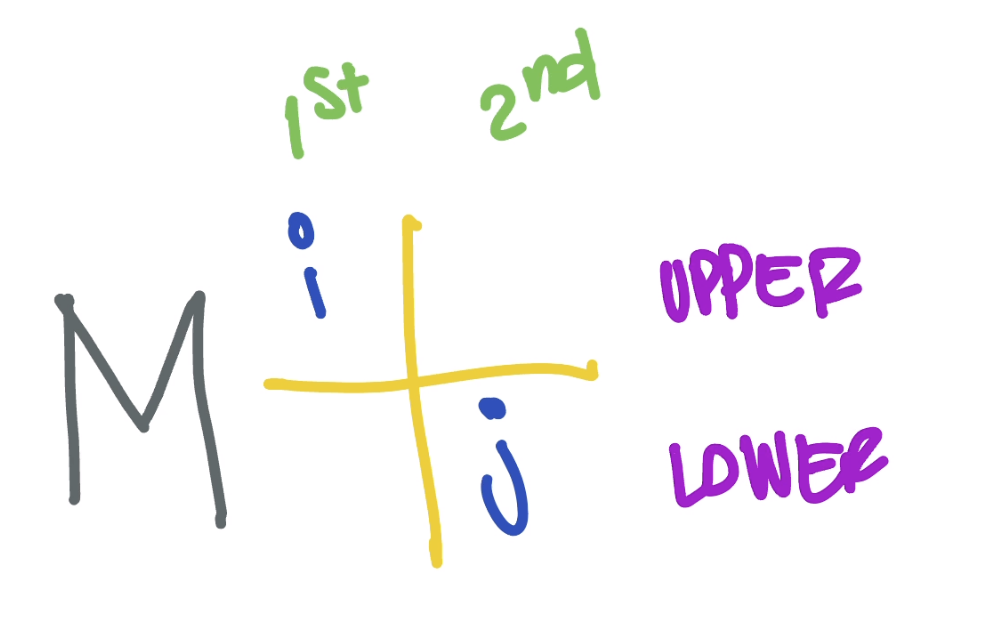
\includegraphics[width=.7\textwidth]{figures/Mij_indices.png}
    \captionsetup{font={scriptsize,sf}}
    \caption{The index placement for a matrix.}
    \label{fig:Mij:index:heights}
\end{marginfigure}
You can take linear combinations of matrices in the same way you take linear combinations of vectors, as per Rule~\ref{rule:vector:linear:combinations}. That is, given two matrices $M$ and $N$, the $ij$-component of the sum of these matrices is
\begin{align}
    (M+N)\aij{i}{j} = M\aij{i}{j} + N\aij{i}{j} \ .
\end{align}
The extension to linear combinations (including rescaling) is trivial.\sidenote{Trivial is how mathematicians say `obvious.' If this point is not obvious, take a moment to see if there is a better way to think about this.}
\begin{example}
Matrices can also be interpreted as vectors. If the index $i$ can run from $1$ to $N$, then a matrix can be understood as an $N^2$-component object. For $2\times 2$ matrices, we could write
\begin{align}
    \vec{v} = 
    \begin{pmatrix}
        v^1 & v^2 \\
        v^3 & v^4
    \end{pmatrix} \ .
\end{align}
In this way, it is a weird repackaging of a 4-component vector. You can check that you can take linear combinations of these `vectors' to form other vectors in the usual way. In this way, the matrix is a repackaging of the components of a vector. Of course, these `vectors' are \emph{completely different} from the 2-component vectors that the $2\times 2$ matrices act on. This identification is rather silly at this point. However, it plays a role in what is called representation theory: the mathematical description of symmetries.
\end{example}

The index structure of matrices means it can contract with both upper-indexed objects like vectors and lower-indexed objects like row vectors. This can happen in several ways. Suppose you have a matrix $M\aij{i}{j}$:
\begin{itemize}
    \item If you also have a row vector $w_i$ and a column vector $v^i$, then you can form a number by contracting them together in the only allowed way: $w_i M\aij{i}{j}v^j$.
    \item If you have a column vector $v^i$, then you can form another column vector by contracting them in the only allowed way: $M\aij{i}{j}v^j$. Observe that this object has one free\sidenote{Here free means uncontracted.} upper index so that it is a column vector.
    \item If you have a row vector $w^i$, then you can form another row vector by contracting them in the only allowed way: $w_iM\aij{i}{j}$. Observe that this object has one free lower index so that it is a row vector.
    \item If you only have the matrix $M\aij{i}{j}$, you can form a number by contracting its two indices, $M\aij{i}{i}$. This is called the \textbf{trace}\index{trace} of the matrix.
\end{itemize}
You can easily understand the first three contractions from your intuition using the matrix multiplication language of Section~\ref{sec:matrix:multiplication},
\begin{align}
    \row{w} M \vec{v} &= 
    \begin{pmatrix}
        w_1 & w_2
    \end{pmatrix}
    \begin{pmatrix}
        M\aij{1}{1} & M\aij{1}{2}\\
        M\aij{2}{1} & M\aij{2}{2}
    \end{pmatrix}
    \begin{pmatrix}
        v^1 \\ v^2
    \end{pmatrix}
    =  
    w_i M\aij{i}{j} v^j
    \\
    \row{w} M &= 
    \begin{pmatrix}
        w_1 & w_2
    \end{pmatrix}
    \begin{pmatrix}
        M\aij{1}{1} & M\aij{1}{2}\\
        M\aij{2}{1} & M\aij{2}{2}
    \end{pmatrix}
    =  
    \begin{pmatrix}
        w_i M\aij{i}{1} & w_i M\aij{i}{2}
    \end{pmatrix}
    \\
    M\row{v} &= 
    \begin{pmatrix}
        M\aij{1}{1} & M\aij{1}{2}\\
        M\aij{2}{1} & M\aij{2}{2}
    \end{pmatrix}
    \begin{pmatrix}
        v^1 \\ v^2
    \end{pmatrix}
    =  
    \begin{pmatrix}
        M\aij{1}{i}v^i \\ M\aij{2}{i}v^i
    \end{pmatrix} \ .
\end{align}
But here we see something powerful about the index notation: in matrix notation, it \emph{does not} make sense to act on a row vector with a matrix `from the right,'
\begin{align}
    M\row{w} = ? \ .
\end{align}
However, from an index point of view:
\begin{align}
    M\aij{i}{j}w_i = w_i M\aij{i}{j} \ .
\end{align}
This is because $M\aij{i}{j}$ is not the matrix $M$, it is a specific \emph{component} of the matrix $M$. As such, it is just a number and multiplication of numbers is commutative.\sidenote{I refer back to Section~\ref{sec:treachery:of:indices:vi:is:not:a:vector}.} Similarly,
\begin{align}
    M\aij{i}{j}v_j = v_j M\aij{i}{j} \ ,
\end{align}
and
\begin{align}
    w_i M\aij{i}{j}v_j = v_j w_i M\aij{i}{j} = v_j  M\aij{i}{j} w_i \ ,
\end{align}
and so forth. This is not `breaking' anything. In fact, our indexology rules are highlighting that it is the matrix multiplication language of Section~\ref{sec:matrix:multiplication} that is limited. 

We re-iterate once more:
\begin{newrule}[Contracted indices] The type of object (tensor) that you have after performing an contraction is determined by the leftover \emph{uncontracted} indices.
\end{newrule}
This means that the trace, $M\aij{i}{i}$ is a number because it has no free (uncontracted) indices. It also means that a matrix acting on a vector $M\aij{i}{j}v^j$ is a vector because it has one free upper index. Of course, we can also imagine other types of objects that return something different when contracting with a vector.

\paragraph{Matrix multiplication} In terms of index notation, matrix multiplication is the contraction of the upper index of one matrix with the lower index of the other. If we multiply matrices $M$ and $N$ in that order, then the $i$--$j$ component of the product is:
\begin{align}
    (MN)\aij{i}{j} =   M\aij{i}{k} N\aij{k}{j}  = N\aij{k}{j} M\aij{i}{k} \ .\label{eq:multiplication:MN:indices}
\end{align}
The second equality here is simply a statement that the product of \emph{numbers} is commutative. Explicitly for the two dimensional case:
\begin{align}
    (MN)\aij{i}{j} &= 
    M\aij{i}{1} N\aij{1}{j} + M\aij{i}{2} N\aij{2}{j}\\
    &=
    N\aij{1}{j} M\aij{i}{1}  + N\aij{2}{j} M\aij{i}{2} \ .
\end{align}
Be sure to read this carefully. Equation \eqref{eq:multiplication:MN:indices} does \emph{not} mean that matrix multiplication is commutative, in particular:
\begin{align}
    N\aij{k}{j} M\aij{i}{k} \neq (NM)\aij{i}{j} \ .
\end{align}
\begin{exercise}
Write out $(NM)\aij{i}{j}$ and confirm that the index contractions are \emph{not} the same as $N\aij{k}{j} M\aij{i}{k}$.
\end{exercise}
What should we make of all this? When we write $MN$ we are implicitly using the matrix multiplication convention of Section~\ref{sec:matrix:multiplication}. Thus $MN$ is \emph{different} from $NM$, as you can check by expanding out the indices.\sidenote{Please do this for a pair of $2\times 2$ matrices if this is not yet clear.} However, index notation tells us that in the expression for a \emph{component of}, $MN$, that is, in $(MN)\aij{i}{j}$, each term in the sum is simply made up of a product of numbers. That product is commutative. 

To say all this differently: matrix multiplication a~la  Section~\ref{sec:matrix:multiplication} told us that there are two different ways to multiply matrices $M$ and $N$: $MN$ and $NM$. In index notation, we also have two different ways to multiply matrices:
\begin{align}
    M\aij{i}{k}N\aij{k}{j}
    &&\text{and}&&
    M\aij{k}{j}N\aij{i}{k} = N\aij{i}{k}M\aij{k}{j} \ .
\end{align}
These two different index contractions correspond to $MN$ and $NM$ respectively.\sidenote{If this is making you scratch your head or exhale with a deep sigh of ennui, it may help to know that matrix multiplication is still an active field of computational mathematics research.\footnotemark}\footnote{\url{https://www.quantamagazine.org/ai-reveals-new-possibilities-in-matrix-multiplication-20221123/}}



\begin{newrule}[From matrix multiplication to index contraction and back]\label{rule:matrix:multiplication:to:indices:and:back}
To convert from the matrix multiplication picture---where matrices are $N\times N$ blocks of numbers that act on columns according to Figure~\ref{fig:matrix:col:mult}---to index notation: first write out all objects with explicit indices. Matrix multiplication corresponds to the contraction of consecutive indices, for example $A\vec{v} = A\aij{i}{j}v^j$. Once you have written everything in terms of indices, you can move factors around: $A\aij{i}{j}v^j = v^jA\aij{i}{j}$ because there is no ambiguity which indices are contracted.

To go from index notation back to matrix multiplication, arrange all contractions so that they are consecutive and interpret consecutive contractions as matrix multiplications. For example:
\begin{align}
     A\aij{i}{j}v_j  w_i =
     w_i A\aij{i}{j} v_j = \row{w} A \vec{v} 
     = 
     \begin{pmatrix}
         w_1 & w_2 
     \end{pmatrix}
     \begin{pmatrix}
         A\aij{1}{1} & A\aij{1}{2}\\
         A\aij{2}{1} & A\aij{2}{2}
     \end{pmatrix}
     \begin{pmatrix}
         v^1\\
         v^2
     \end{pmatrix}
     \ .
\end{align}
It does not matter if you contract lower indices to upper indices or upper indices to lower indices as you read from left-to-right, only that the indices are consecutive. 

\textbf{Caveats}: sometimes different tensor contractions appear to give the same matrix multiplication. Usually in these cases the type of contraction is formally not allowed in the limited matrix multiplication picture. For example, $w^iv^j g_{ij}$ is a valid tensor contraction involving two vectors and an object with two lower indices. It cannot be written as a matrix multiplication without breaking the rules.
\end{newrule}



\paragraph{Matrix inverses}
We touched on inverse matrices in \eqref{eq:matrix:invers:multiplcation:notation}. Let us return to it using index notation. \emph{If} a matrix is invertible, then the condition \eqref{eq:matrix:invers:multiplcation:notation} is
\begin{align}
    M\aij{i}{k}(M\inv)\aij{k}{j} = (M\inv)\aij{i}{k}M\aij{k}{j} = \delta^i_j
    \label{eq:index:matrix:inverse}
\end{align}
where we define the Kronecker-$\delta$,\sidenote{The Kronecker-$\delta$ are the components of the identity matrix. Because it is diagonal, the order of the indices does not matter so we can write both indices with the same horizontal alignment. In a contraction, the Kronecker-$\delta$ simply says: replace a sum over one of my indices with the value of the other index.}
\begin{align}
    \delta^i_j = \begin{cases}
    1 & \text{if } i=j \\
    0 & \text{otherwise .}
    \end{cases}
    \label{eq:kronecker:delta}
\end{align}
If the indices can take values from 1 to $N$, then there are $N^2$ equations to constrain the $N^2$ components of $M\inv$. If the matrix $M$ is invertible, then one could solve this system of equations to determine $M\inv$. In silly versions of this course, one would spend time using some software---perhaps Matlab---to solve this system of equations. That's silly. Matrices are either invertible by hand, easy to invert using your favorite computer algebra system\sidenote{\emph{Mathematica} is popular among theorists, though \emph{NumPy} and \emph{SciPy} are both open source.}, or so hopelessly impossible to invert that other techniques are needed to approximate their inversion.\sidenote{Taylor expansions about an easier-to-invert matrix, for example.} However, understanding what it means to invert a matrix is a \emph{big} part of mathematical physics. In fact, it is a central thrust of physics.
\begin{bigidea}\label{idea:matrix:inverse:in:physics}
A surprisingly large swath of physics---and certainly the part that is most do-able---boils down to inverting matrices of various (often infinite) sizes. This is because equations in physics are often in the form
\begin{align}
    (\text{operator})\, \ket{\text{state}} = \ket{\text{source}} \ .
\end{align}
We have used ket notation, but recall that these are just vectors. Usually you know what the operator (matrix) is and you know what the source is. For example, the operator may be some vector calculus operator, perhaps the divergence. The source is usually a physical configuration, perhaps the density of charge. Then the state---which is what you want to find---would be the electric field. The general solution to problems in this form is
\begin{align}
 \ket{\text{state}} = (\text{operator})\inv\, \ket{\text{source}} \ .
\end{align}
And it thus behooves us to understand what it means to invert an operator. So another way to think about our course, ``linear algebra for physicists,'' is to say it is the toolkit to invert operators that show up in physics.
\end{bigidea}

\subsection{Tensors}
\label{sec:index:tensors:rotation:on:each:index}

A \textbf{tensor}\index{tensor} is an object with some number of ordered indices. Each index has a definite height. We say that a tensor is a $(p,q)$ tensor if it has $p$ upper indices and $q$ lower indices. Vectors, row vectors, and matrices are all tensors. We met an example of a different type of tensor in Figure~\ref{fig:Riemann:tensor:for:indices}, the Riemann tensor,\sidenote{In general relativity (differential geometry) this tensor takes in three vectors and returns another vector. The first two vectors are sides of a parallelogram. In a general curved space, one cannot close this parallelogram. If we take the third vector and `transport it' along the two paths of the parallelogram, the difference in what happens to the third vector is what the Riemann tensor returns. See Figure~\ref{fig:Penrose:14:10:Riemann}.} $R^i_{\phantom{i}jk\ell}$. What can this object do? 
\begin{marginfigure}%[th]
    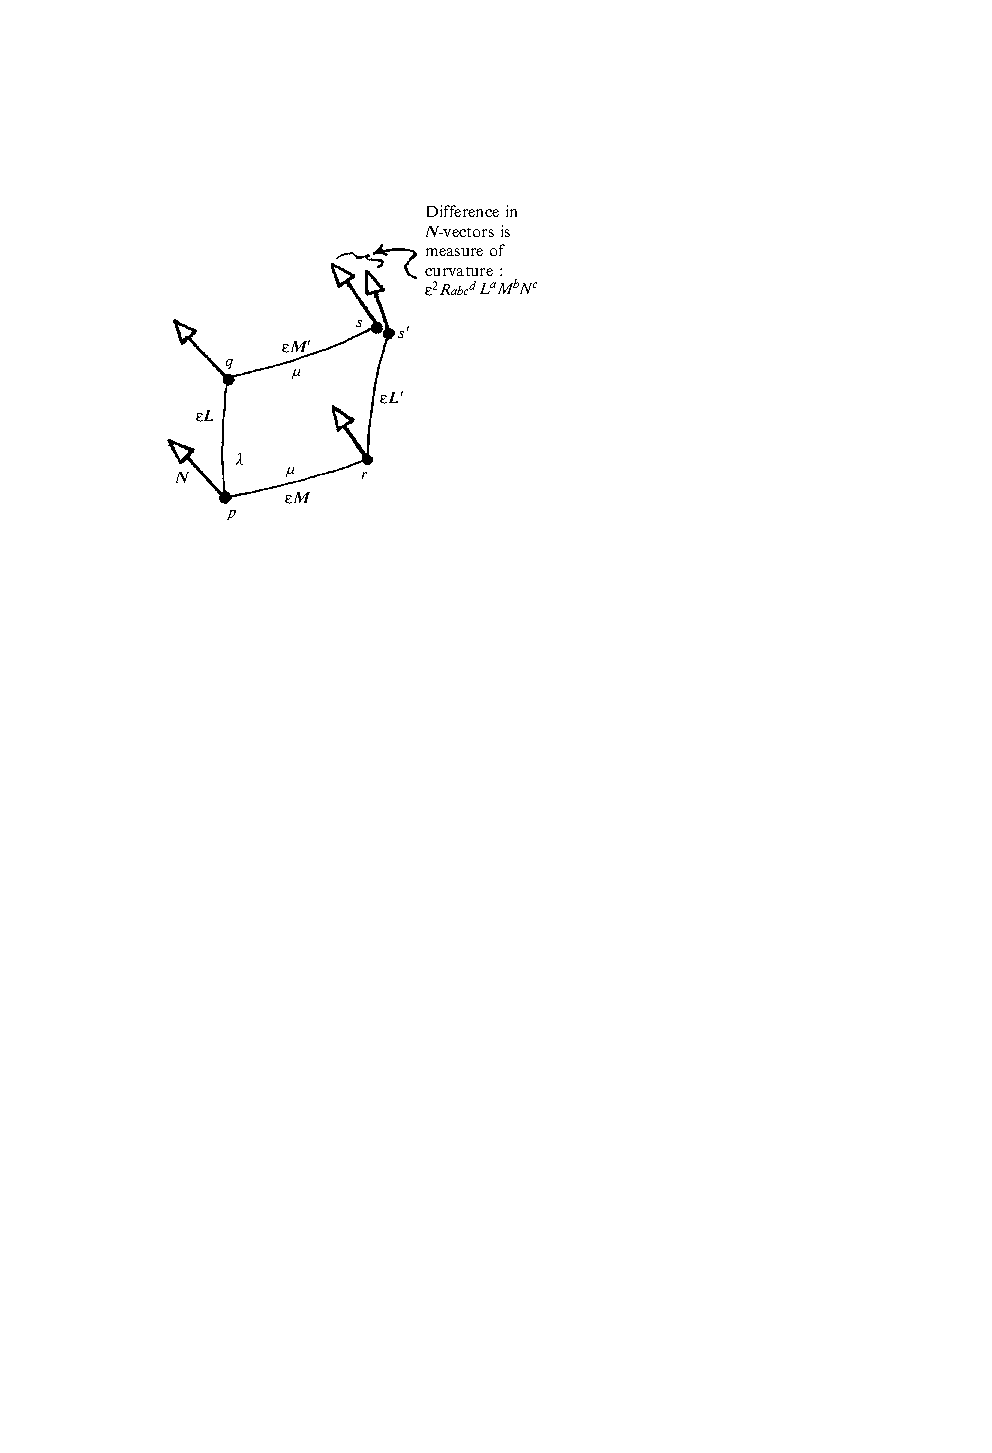
\includegraphics[width=.8\textwidth]{figures/Penrose_Riemann_14_10.pdf}
    \captionsetup{font={scriptsize,sf}}
    \caption{Graphical depiction of what the Riemann tensor from Penrose, \emph{Road to Reality}. Note that Penrose uses a different ordering of indices than we do.}
    \label{fig:Penrose:14:10:Riemann}
\end{marginfigure}
Based on the index structure alone, you can determine that the Riemann tensor can:
\begin{itemize}
    \item Take three vectors and a row vector to return a number, $R^i_{\phantom{i}jk\ell} v^jw^ku^\ell t_i$.
    \item Take two vectors and return a matrix, $R^i_{\phantom{i}jk\ell}v^kw^\ell$. 
    \item Take two vectors and a row vector to return a row vector, $R^i_{\phantom{i}jk\ell}w_iv^ju^k$.
    \item ... and a few more that you can write out. Do not forget contractions of the upper index with one of the lower indices.
\end{itemize}
\begin{newrule}[Tensor contractions]
A $(p,q)$ tensor can contract with $r\leq p$ row vectors and $s \leq q$ column vectors to produce a $(p-r, q-s)$ tensor. By allowing `traces' of the tensor's own upper and lower indices, you can also produce $(p-r-n, q-s-n)$ tensors so long as $p-r-n\geq 0$ and $q-s-n\geq 0$.
\end{newrule}
\begin{exercise}
You can generalize the above rule by allowing a $(p_1,q_1)$ tensor to contract with a $(p_2, q_2)$ tensor. Write out some of the ways in which a $(2,2)$ tensor can contract with a $(1,3)$ tensor. Here is one example: $T^{ij}_{\phantom{ij}k\ell} S^\ell_{\phantom{\ell}ijm}$. 
\end{exercise}
You can see that tensor contraction can get a little dicey. There is a cute graphical notation called birdtracks notation to keep track of this that never became popular.\sidenote{The cover image for these notes is an example of one such contraction. You can learn more about this in Penrose's \emph{Road to Reality}.} In this course we do not worry about very complicated contractions and can stick to index notation.


\subsection{A prelude to symmetry}
\label{sec:isometry:first:pass:indices}
Some ideas are so significant that we introduce them multiple times. Let us preview a key idea: an \textbf{isometry}\index{isometry} is a special symmetry that some vector spaces may have.\sidenote{Specifically, vector spaces equipped with an inner product---called metric spaces---may have isometries.} Let us not concern ourselves for now with the conditions for when such symmetries exist. Instead, for this first pass let us say that isometries are generalizations of rotations.  Take a moment to review the `matrix multiplication' picture of rotations in Section~\ref{sec:Euclidean:three:space:rotations}: rotations $R$ satisfy $R^\trans R = \one$ and, due to this, they preserve the angle and length of vectors. The preservation of angle and length depend on a definition of the dot product---and we are not doing that just yet. However, we can take the lesson that the dot product takes vectors and creates scalars.\sidenote{Scalar is a fancy name for number. More practically, scalars do \emph{not} change under rotations.}

We know that one way to form numbers from objects that have indices is to contract all available indices. Let us examine the simplest such case: a row vector whose indices are contracted with a column vector: $w_iv^i$. Rotations are transformations that act on both row vectors and column vectors. Because row and column vectors are two separate classes of tensorial objects, we allow for the possibility that row vectors and column vectors transform differently:
\begin{align}
    v^i &\to v'^i \defeq R\aij{i}{j}v^j & w_i &= \to w'_j\defeq w_j \tilde{R}\aij{j}{i} \ ,
    \label{eq:components:of:vector:and:row:under:rotatino}
\end{align}
where $R$ and $\tilde{R}$ are the matrices that encode the linear transformation on vectors and row vectors respectively.\sidenote{Neither of these have anything to do with the Riemann curvature tensor, which unfortunately is denoted with an $R$.} We write $v'^i$ and $w'_j$ to be the components of the rotated $v^i$ and $w_j$. Inspired by our earlier intuition that rotations should preserve the value of `fully contracted' objects,\sidenote{All tensor indices are contracted, no free indices.} we can demand that
\begin{align}
    w_i v^i =w'_i v'^i = R\aij{i}{j}v^j \, w_k\tilde{R}\aij{k}{i}
    =\tilde{R}\aij{k}{i}R\aij{i}{j} w_kv^j \ .
    \label{eq:rotations:index:preserve:inner:product:01}
\end{align}
Let us do something silly. We would like to `do algebra' on this equation, which means I would like to cancel out common factors on each side. I would like to cancel the $w_i$ and $v^i$ on the left with the $w_kv^j$ on the right. I can relabel dummy indices,\sidenote{By `dummy index' I mean contracted indices where the choice of variable name does not matter. Though every time I say `dummy index' I think about the `dummy plug' program in \emph{Neon Genesis Evangelion}.} but we need to break apart the fact that $w_i$ and $v^i$ have the same index on the left-hand side. To do this, we multiply by one using the Kronecker-$\delta$: $w_iv^i = w_i \delta^i_j v^j$. Then we may rewrite  \eqref{eq:rotations:index:preserve:inner:product:01} as
\begin{align}
    \cancel{w_i} \cancel{v^j}  \delta^i_j
    =\tilde{R}\aij{i}{\ell}R\aij{\ell}{j} \cancel{w_i} \cancel{v^j} \ ,
\end{align}
from which we have simply:
\begin{align}
    \tilde{R}\aij{i}{\ell}R\aij{\ell}{j} &= \delta^i_j \ .
    \label{eq:R:Rtilde:transformation:from:indices:rotation}
\end{align}
Comparing to \eqref{eq:index:matrix:inverse}, we see that this is the statement that $\tilde R = R\inv$. We have come to a key observation:
\begin{quote}
Under a rotation, an object with an upper index transforms with some matrix $R$ that encodes the rotation. An object with a lower index then transforms with the inverse matrix, $R\inv$. In this way, when a row vector and column vector have their indices contracted, they produce a number that is \emph{invariant} (unchanged) under rotations.
\end{quote}
This observation actually generalizes:
% 
\begin{newrule}[Transformation of upper and lower indices under rotations]
\label{idea:transformation:of:upper:and:lower:indices}
Under an isometry (such as a rotation) $R$, a tensorial object transforms as follows
\begin{align}
    T\aij{i_1\cdots i_N}{j_1\cdots j_M}
    \to 
    R\aij{i_1}{k_1}\cdots R\aij{i_N}{k_N}
    (R\inv)\aij{\ell_1}{j_1}\cdots (R\inv)\aij{\ell_M}{j_M}
    T\aij{k_1\cdots k_N}{\ell_1\cdots \ell_M} \ .
    \label{eq:transformation:of:upper:and:lower:indices}
\end{align}
That is to say: each upper index is contracted with a rotation $R$ and each lower index is contracted with an inverse rotation $R\inv$. 
\end{newrule}

\begin{exercise}
Show that for the case of $2\times 2$ rotations, the inverse is equivalent to the transpose. This turns out to be true for any rotation matrix in Euclidean space.
\end{exercise}

\begin{exercise}
Show that our rule for how row vectors transform can be written in matrix notation as:
\begin{align}
    \row{w} \to \row{w}' \equiv \row{w} R^\trans \ .
\end{align}
To do this, show that the index contracts correspond to the right-hand side. Use the result of the previous exercise that $R\inv = R^\trans$ for rotations.
In this way, it is clear that $\row{w}\vec{v} = \row{w'}\vec{v'}$ is invariant under rotations:
\begin{align}
    \row{w'}\vec{v'} = \row{w}R^\trans R\vec{v} = \row{w} \one \vec{v} \ ,
\end{align}
where we use the definition \eqref{eq:RTR:one}.
\end{exercise}





\section{Vector Space}

If you have some vectors, the combined set of all possible linear combinations of those vectors is called a \textbf{vector space}. This is the idea introduced in Section~\ref{sec:linear:combination:and:span}. Suppose you have some vectors\sidenote{Note that the lower index here is \emph{not} a component index! The vector $\vec{v_2}$ has components $(v_2)^1, (v_2)^2, \cdots$.},  $\vec{v}_1, \cdots, \vec{v}_N$. From these vectors, you can form an infinite number of other vectors by choosing numbers $\alpha^i$ and forming the linear combination
\begin{align}
    \alpha^1 \vec{v}_1 + \alpha^2\vec{v}_2 + \cdots + \alpha^N \vec{v}_N \ .
    \label{eq:linear:combination:looks:like:basis}
\end{align}
The set of all possible vectors that can be formed this way is called the \textbf{vector space} \emph{spanned by}  $\vec{v}_1, \cdots, \vec{v}_N$. The word \textbf{span}\index{span} means the vector space of all linear combinations of a set of vectors. When we say that \emph{linear combinations of vectors are also vectors}, what we mean is that they are \emph{also vectors in the vector space}. We write vector spaces with a capital letter, say $V$, and write that a vector $\vec{v}$ is part of the vector space by writing
\begin{align}
    \vec{v} \in V \ .
\end{align}

\begin{example}
If you have two vectors,
\begin{align}
    \vec{v} &= 
    \begin{pmatrix}
        3 \\ 1 \\ 0
    \end{pmatrix}
    &
    \vec{w} &= 
    \begin{pmatrix}
        2 \\ 1 \\ 3
    \end{pmatrix}
    \label{eq:eg:of:vector:space:1}
\end{align}
then you could form another vector that is a linear combination of the two:
\begin{align}
    2\vec{v} - 1 \vec{w}
    =
    \begin{pmatrix}
        4 \\ 1 \\ -3
    \end{pmatrix} \ .
\end{align}
We say that this vector is part of the vector space $V$ spanned by $\vec{v}$ and $\vec{w}$. 
\end{example}

\begin{example}
If $V$ is the vector space spanned by by $\vec{v}$ and $\vec{w}$ in \eqref{eq:eg:of:vector:space:1}, then the vector
\begin{align}
    \vec{u}
    =
    \begin{pmatrix}
        3 \\ 1 \\ 2
    \end{pmatrix} \ .
\end{align}
is \emph{not} part of the vector space $V$ because there are no coefficients $\alpha^1$ and $\alpha^2$ that can satisfy
\begin{align}
    \alpha^1\vec{v} + \alpha^2 \vec{w} = \vec{u} \ .
\end{align}
If you are not convinced, please try it. In the above condition, how many unknowns are there? How many component-level constraint equations are there?
\end{example}

\begin{example}
Consider the vectors
\begin{align}
    \vec{a}
    &=
    \begin{pmatrix}
        1\\0
    \end{pmatrix}
    &
    \vec{b}
    &=
    \begin{pmatrix}
        0\\1
    \end{pmatrix}
    &
    \vec{c}
    &=
    \begin{pmatrix}
        1\\1
    \end{pmatrix}\ .
\end{align}
The vector space spanned by these three vectors is \emph{all} of the two-component vectors. In fact, the vector space spanned by any \emph{two} of these vectors is all of the two-component vectors. 
\end{example}


By this notion of duality, you should expect that row vectors also form a vector space. If the space of column vectors is called $V$, then the space of row vectors is called $V^*$. Evidently there is some relation between the two, even though they appear be totally different vector space.\sidenote{That is: we could have just said that row vectors live in a vector space $W$ and $W$ has nothing to do with $V$.} Indeed, the relation is that that row vectors can contract with column vectors. The star evidently means the space of \emph{vectors that can contract with this other set of vectors}. In this way, column vectors are the dual space of row vectors: $(V^*)^* = V^{**} = V$. This is simply saying that in the contraction $w_i v^i$, we can think of $w_i$ acting on $v^i$ or we can equivalently think of $v^i$ acting on $w_i$. 


\section{Basis of a Vector Space}\label{sec:basis}

Let us return to \eqref{eq:linear:combination:looks:like:basis}. Take a moment to take a good look at that equation. In fact, this equation is so important that we write it out again:
\begin{align}
    \alpha^1 \vec{v}_1 + \alpha^2\vec{v}_2 + \cdots + \alpha^N \vec{v}_N \ .
    \tag{\ref{eq:linear:combination:looks:like:basis}}
\end{align}
Here are a few thoughts that may come to your mind while looking at this linear combination of vectors.
\begin{enumerate}
    \item Hmm. We have $N$ vectors and took a linear combination of them. This means that we needed $N$ coefficients. Rather than writing $\alpha$, $\beta$, $\gamma$, and so forth, we chose to jsut label them all $\alpha$ but with an upper index. 
    \item Oh... the upper index is convenient because it means we can write the linear combination as $\alpha^i \vec{v}_i$. But this isn't a ``real'' contraction, right? Well... it follows the summation convention so I suppose that's legitimate. It is just weird that $\vec{v}_i$ is an entire vector with and additional lower index.
    \item In fact, these $\alpha^i$ coefficient look suspiciously like the components of a vector.
    \item Wait a second, $\alpha^i\vec{v}_i$ \emph{is} a vector.
    \item Can I think about $\alpha^i$ as being the components of the vector $\alpha^i\vec{v}_i$?
\end{enumerate}


\subsection{An understanding between friends}
This brings us to the critical idea of a basis. Now is a good time to go over the examples in the previous section. Go ahead and do that. \emph{Right now.} Okay, welcome back. Suppose that you and I agreed on a set of vectors. Let's say that we both agreed on the $N$ vectors in \eqref{eq:linear:combination:looks:like:basis}; we even agree on the numbering. Let us call this special set of vectors a \textbf{basis}\index{basis}. That means that if I want to communicate to you some linear combination of those vectors, all I have to do is give you a list of their coefficients. I would write this as a column,
\begin{align}
    \vec{a} = 
    \begin{pmatrix}
        \alpha^1\\
        \vdots \\
        \alpha ^N
    \end{pmatrix} \ .
\end{align}
You may say: oh, that's an odd way to write a linear combination---just stacking the coefficients in a column like that. But sure, we both understand that what this \emph{really} means is
\begin{align}
    \vec{a} = 
    \alpha^i \vec{v}_i \ ,
\end{align}
we can just leave the $\vec{v}_i$ implicit because we both already agree on what those vectors are. 

Maybe you see what is going on here. We previously introduced vectors as columns of numbers. Now we are saying that columns of numbers represent a particular linear combinations of basis vectors. It seems that all this time, the `column of numbers' that we started actually mean a linear combination of a specific choice of basis vectors. In fact, the standard or canonical basis vectors can be thought of as columns:
\begin{align}
    \bas{e}_1 &= 
    \begin{pmatrix}
        1\\ 0 \\  0 \\\vdots
    \end{pmatrix}
    &
    \bas{e}_2 &= 
    \begin{pmatrix}
        0 \\ 1 \\  0 \\\vdots
    \end{pmatrix}
    &
    \bas{e}_3 &= 
    \begin{pmatrix}
        0 \\ 0 \\  1 \\\vdots
    \end{pmatrix}
    &
    \cdots
    \label{eq:canonical:basis}
\end{align}
We have moved to a notation where we write the basis vectors as $\bas{e}_i$. A basis does not \emph{need} to be nice. 


In terms of the canonical basis \eqref{eq:canonical:basis}, we now understand that the components of a vector mean
\begin{align}
    \vec{v} = v^1 \bas{e}_1 + v^2 \bas{e}_2 + \cdots = v^1 \bas{e}_1 \ .
\end{align}

\begin{bigidea}[The big deal about bases]\label{idea:reasons:to:like:bases}
This whole hubbub about bases is useful for at least two reasons:
\begin{enumerate}
    \item This notion completely abstracts away the \emph{meaning} of a vector. The basis vectors carry all the `vector-ness'\sidenotemark of the vector. 
    \item If you and I are \emph{not} using the same basis, then all I have to do is convert your basis into my basis to be able to convert your components into my components.
\end{enumerate}
\end{bigidea}\sidenotetext{Or more generally, tensor-ness.}

We briefly introduce these two ideas in turn. But first, let us address the index structure of the basis.

\paragraph{Why do basis vectors have lower indices?} Previously we said objects with a single lowered index are row vectors. Are basis vectors row vectors? Not quite. In fact, when we talked about tensors, we said that the specific component $T^{i_1\cdots i_N}_{\phantom{{i_1\cdots i_N}}j_1\cdots j_M}$ is just some number. For basis vectors, once we specify $i$, $\bas{e}_i$ is \emph{not} a number: it carries all of the \emph{meaning} of what a vector \emph{is} in whatever context the vector is being used. The basis vector has a lower index because it means we can contract it with the upper index of $v^i$. The resulting object is the vector itself, $\vec{v}$ which carries no indices. If this sounds like philosophical navel gazing, please jump ahead and do Exercise~\ref{ex:fibonacci:space}---it is a rather different example of `vector-ness' than `columns of numbers.'





\subsection{Abstraction}
\label{sec:sub:abstraction:basis}

% In Section~\ref{sec:sub:basis:changing} we saw how making the basis vectors explicit helps us understand how to relate tensors in one reference frame (basis) to another. Recall that there is a second reason in \bigidearef~\ref{idea:reasons:to:like:bases} why basis vectors are helpful: they
Basis vectors help us further let vectors become more abstract.\sidenote{There is an analogy here to the \LaTeX typesetting system. The goal of \LaTeX is to separate content from the under-the-hood work to present that content. For practical purposes, we want to separate components---which are just numbers that we can work with---from underlying mathematical machinery that gives those components meaning.}
%
Another way of saying this is as follows:
\begin{quote}
Vectors are \emph{not} columns of numbers.
\end{quote}
Those numbers are the \emph{components} of a vector. But the \emph{meaning} of a vector depends on the context. In some contexts the vector might be a velocity or a momentum. It may be a unit excitation in the electric field. It may be the spin state of an electron. It may be a solution to the spherical Laplace equation. The magic is that all sorts of \emph{physical} quantities are described by vectors. The basis vectors carry these identities so that we can just work with numerical coefficients that we happen to denote with upper indices and that we sometimes arrange in columns.


\paragraph{Arrow space}
Our goal is to abstract away any notion of column vectors. A useful way to think about this is an idea that is perhaps familiar: imagine vectors are arrows with a magnitude and a direction. The rule for adding vectors is that you stack them together, tail-to-head.\sidenote{It should be clear that this definition is commutative, $\vec{v}+\vec{w} = \vec{w}+\vec{v}$.} For example, consider the following basis:
\begin{align}
    \bas{e}_1 &= \eqfig{
\includegraphics[width=2em]{figures/basis_e1.pdf}}
    &
    \bas{e}_2 &= \eqfig{
\includegraphics[width=2em]{figures/basis_e2.pdf}} \ .
\end{align}
Then a vector $\vec{v}$ may be written as a linear combination of those vectors. Figure~\ref{fig:eg:basis:arrows:canonical:eg} demonstrates this.
\begin{marginfigure}%[th]
    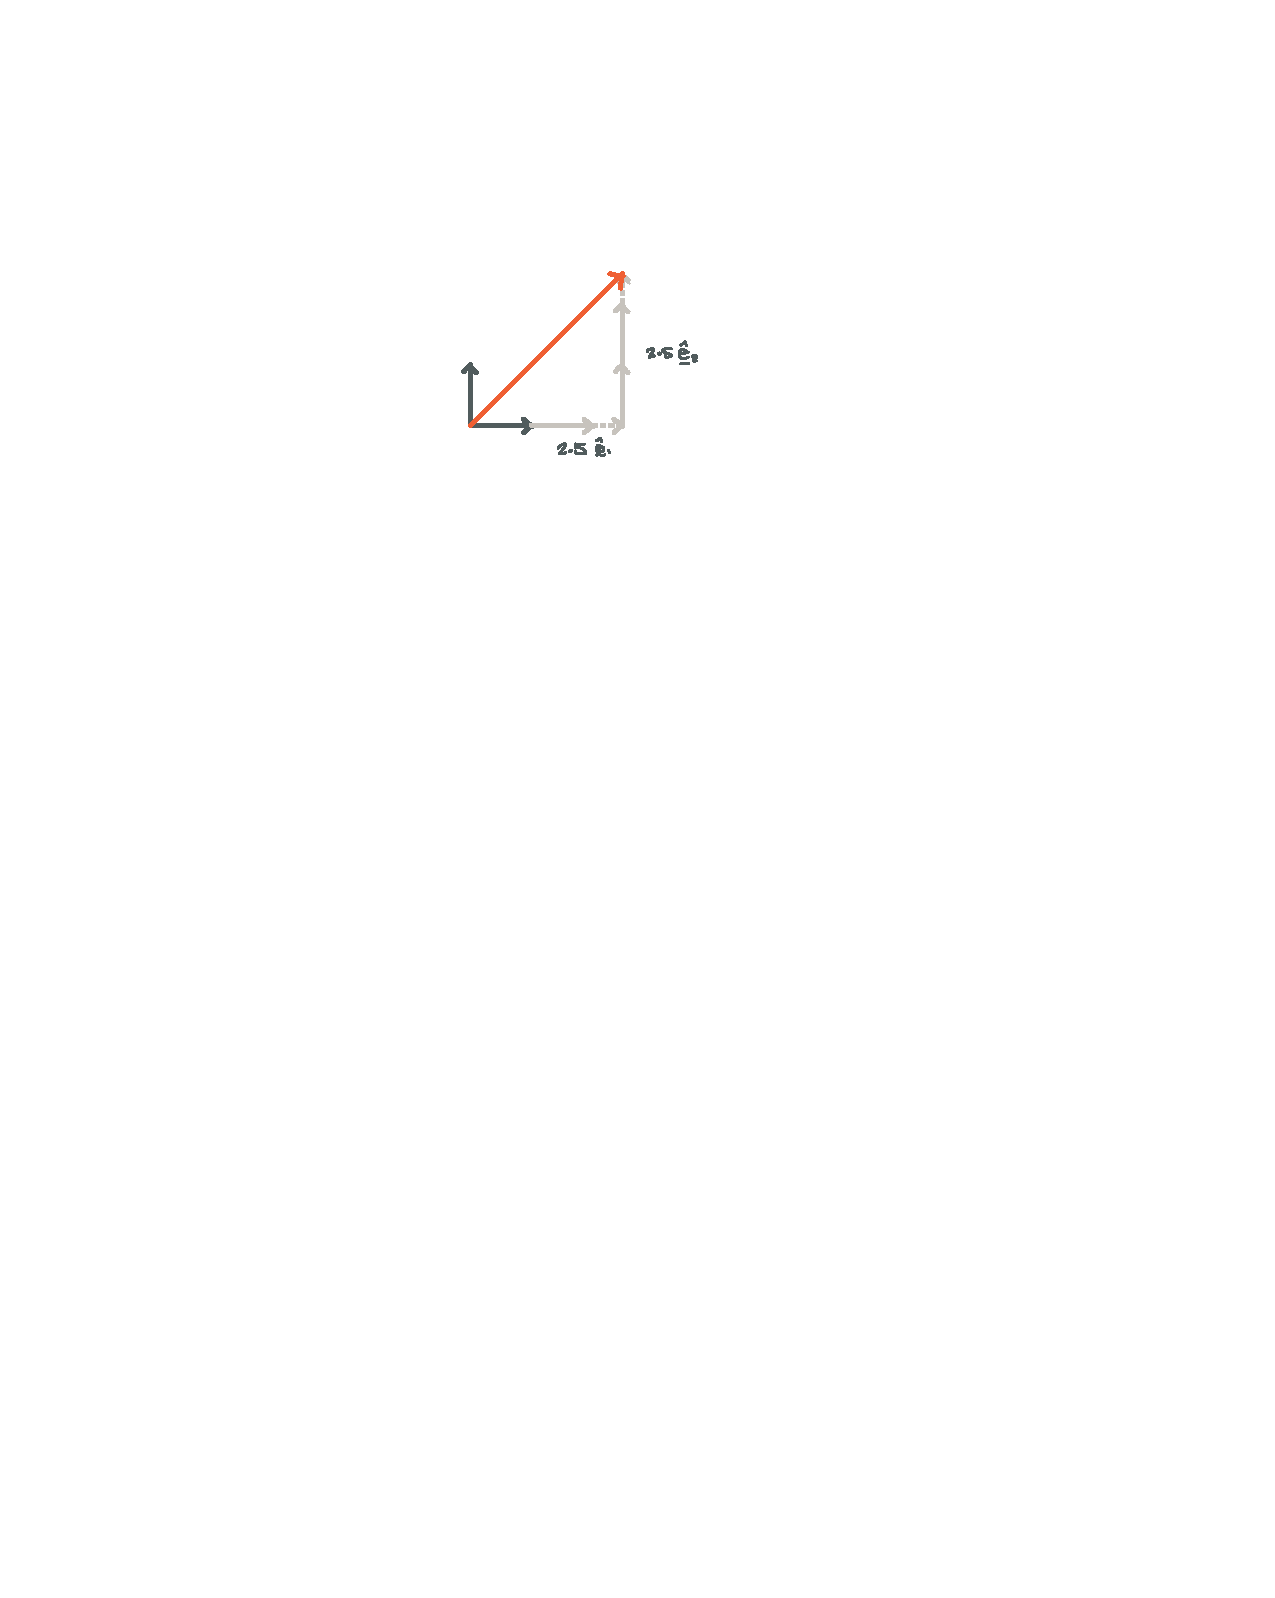
\includegraphics[width=.6\textwidth]{figures/basis_red_e.pdf}
    \captionsetup{font={scriptsize,sf}}
    \caption{The vector $\vec{v}$ (in red) is $2.5\bas{e}_1 + 2.5\bas{e}_2$.}
    \label{fig:eg:basis:arrows:canonical:eg}
\end{marginfigure}
In that example, the components of the vector $\vec{v}$ are
\begin{align}
    \vec{v} &= v^i\bas{e}_i = 2.5 \bas{e}_1 + 2.5 \bas{e}_2  \ .
\end{align}
We could have used a different basis of the same space. This basis is
\begin{align}
    \bas{f}_1 &= \eqfig{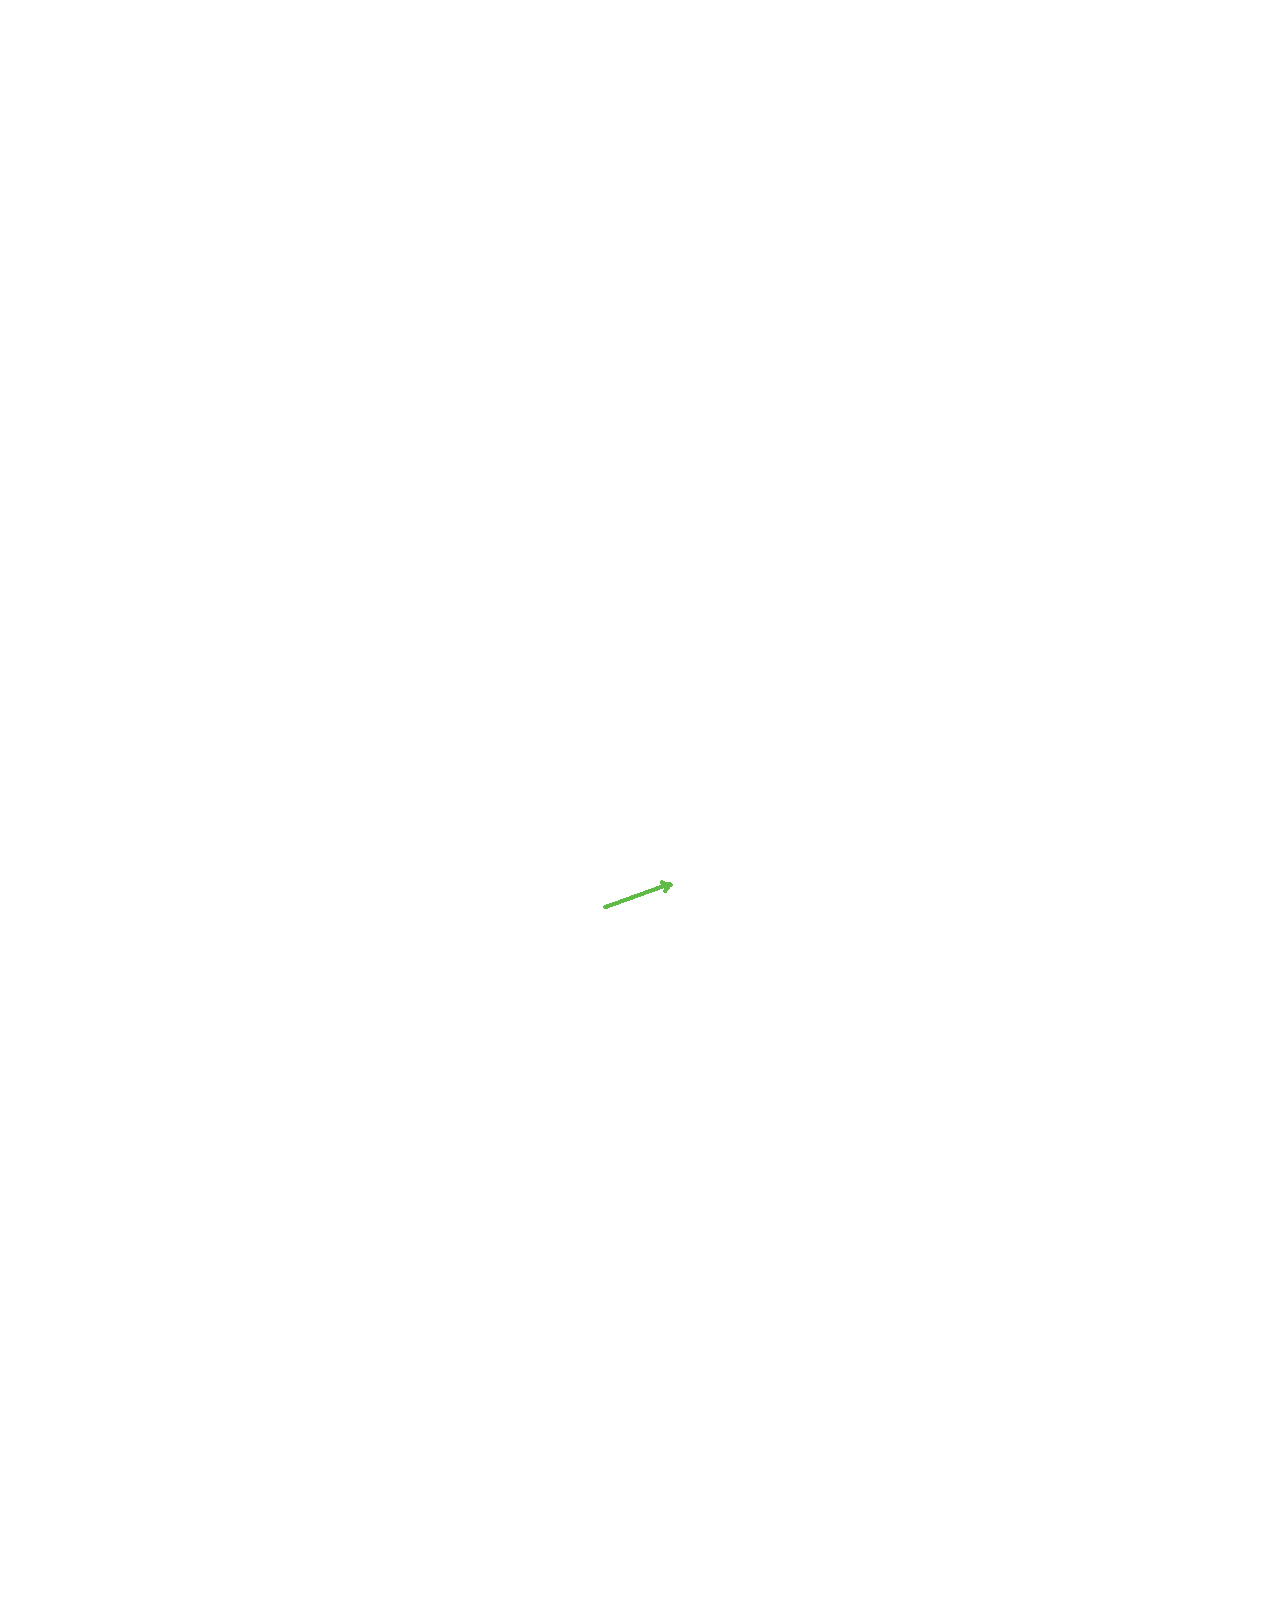
\includegraphics[width=2em]{figures/basisf1.pdf}}
    &
    \bas{f}_2 &= \eqfig{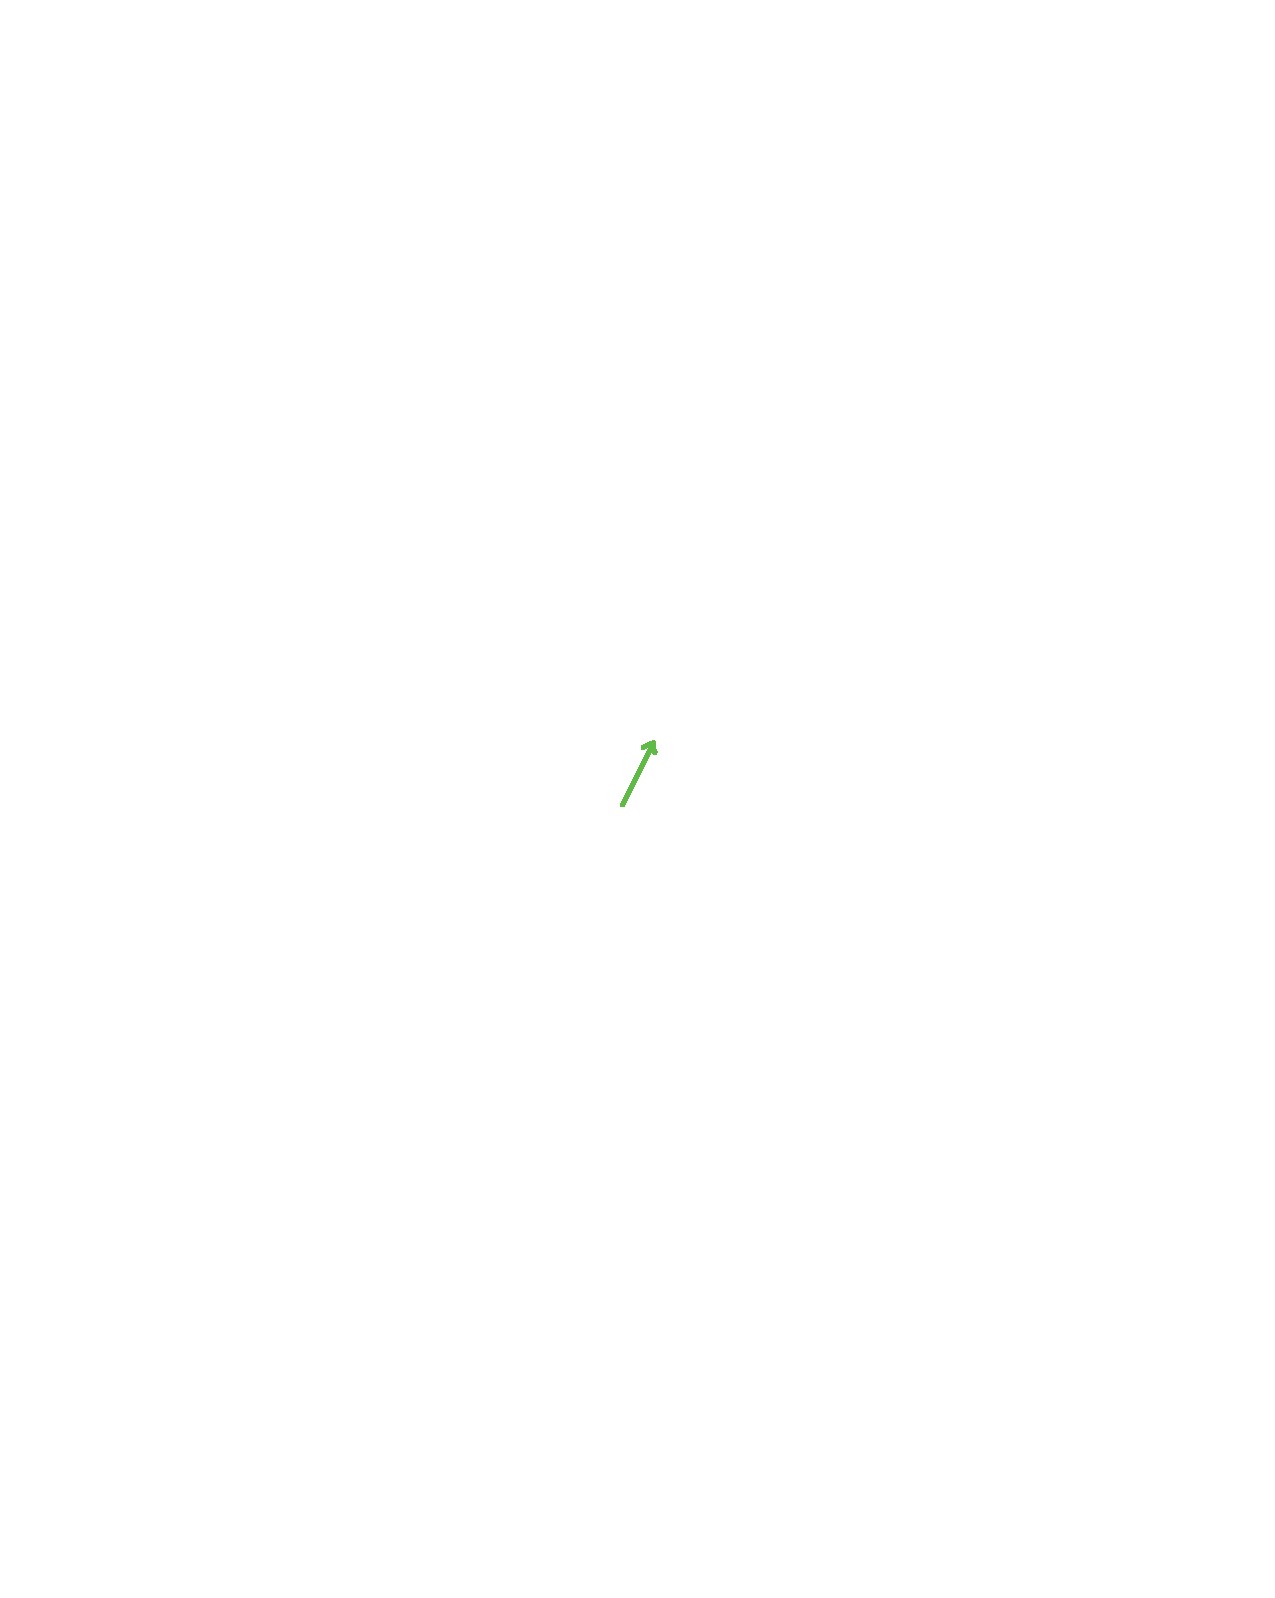
\includegraphics[width=2em]{figures/basisf2.pdf}} \ .
\end{align}
Figure~\ref{fig:eg:basis:arrows:canonical:eg:odd:basis} shows the same vector $\vec{v}$ written as a linear combination of the $\bas{f}_{1,2}$ basis.
\begin{marginfigure}%[th]
    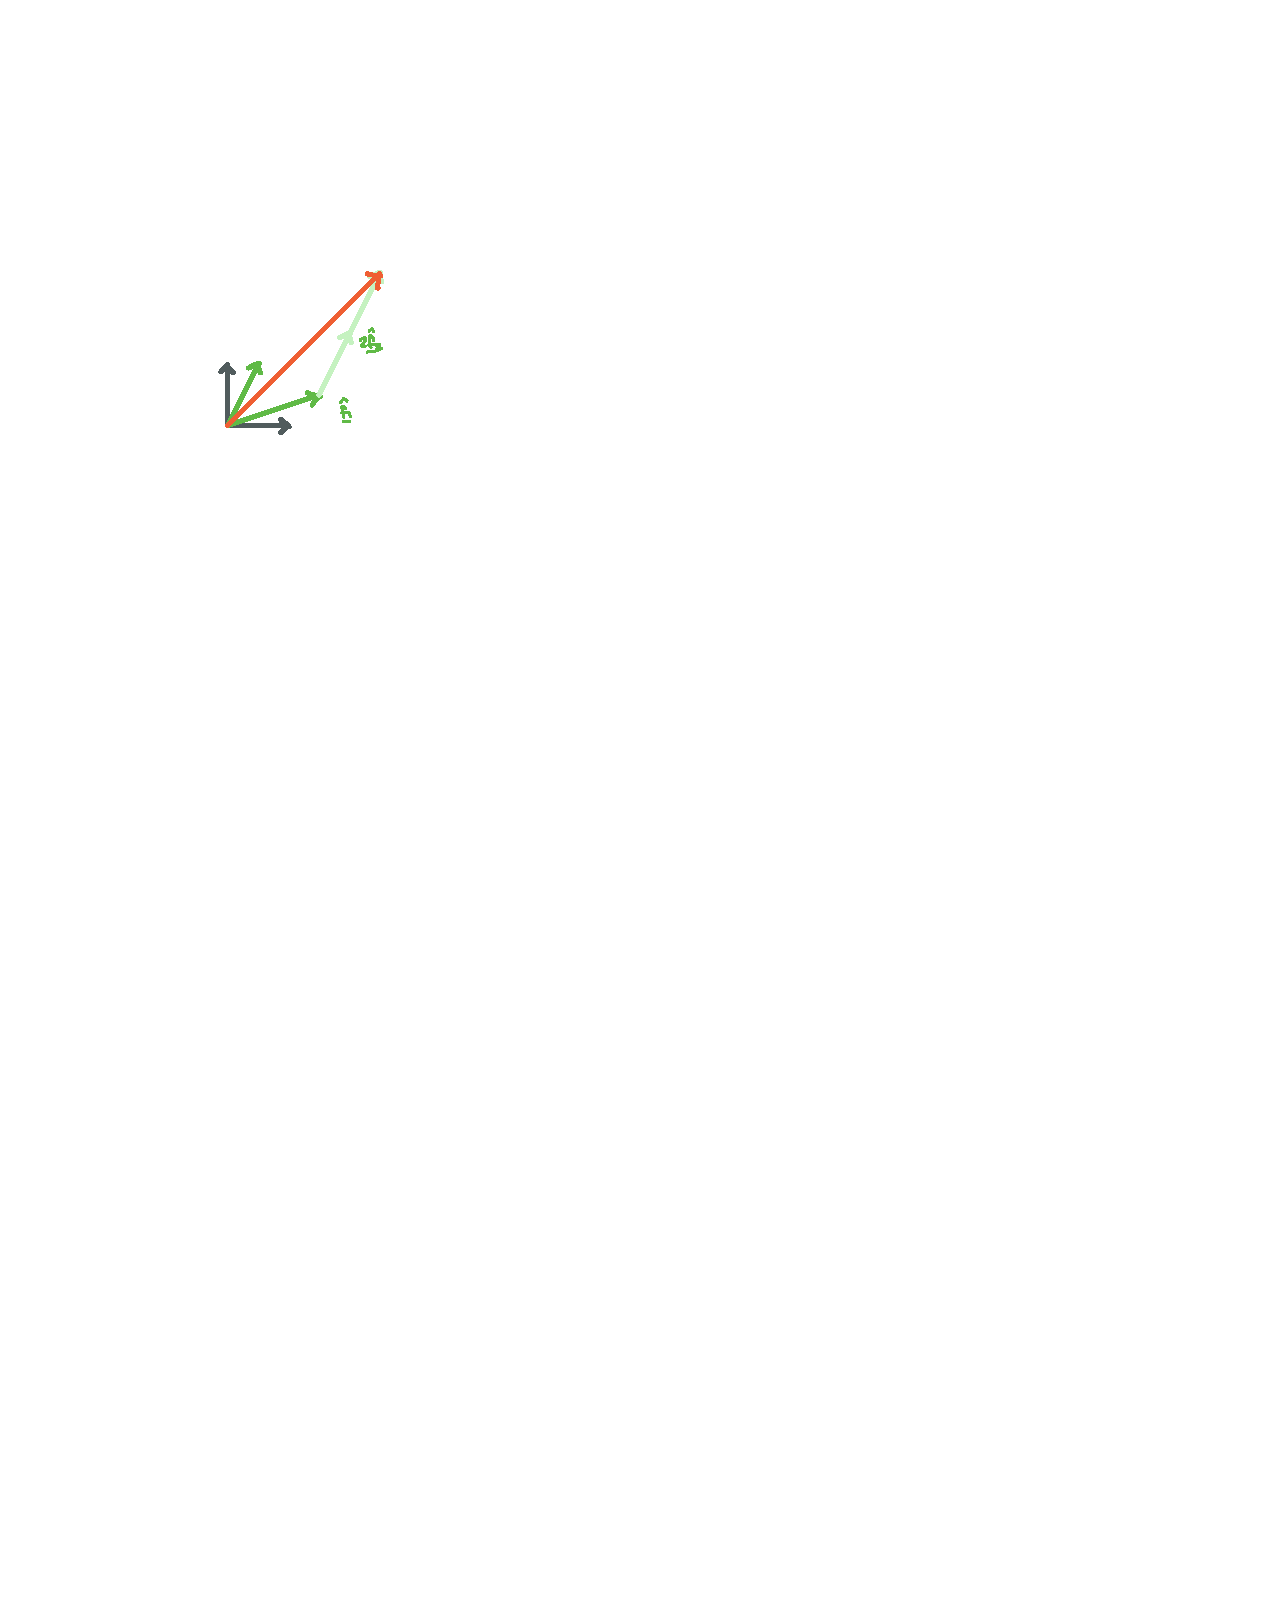
\includegraphics[width=.6\textwidth]{figures/basis_red_f.pdf}
    \captionsetup{font={scriptsize,sf}}
    \caption{The vector $\vec{v}$ (in red) is $\bas{f}_1 + 2\bas{f}_2$.}
    \label{fig:eg:basis:arrows:canonical:eg:odd:basis}
\end{marginfigure}
\begin{align}
    \vec{v} &= v'^i\bas{f}_i =  \bas{f}_1 + 2\bas{f}_2  \ .
\end{align}

As a final demonstration, we illustrate that coefficients of basis vectors may also be negative. In Figure~\ref{fig:eg:basis:arrows:neg} we have a vector in blue that is a positive sum of the $\bas{e}_{1,2}$ basis vectors, but is the linear combination $3\bas{f}_1 - \bas{f}_2$ in the $\bas{f}_{1,2}$ basis.
\begin{marginfigure}%[th]
    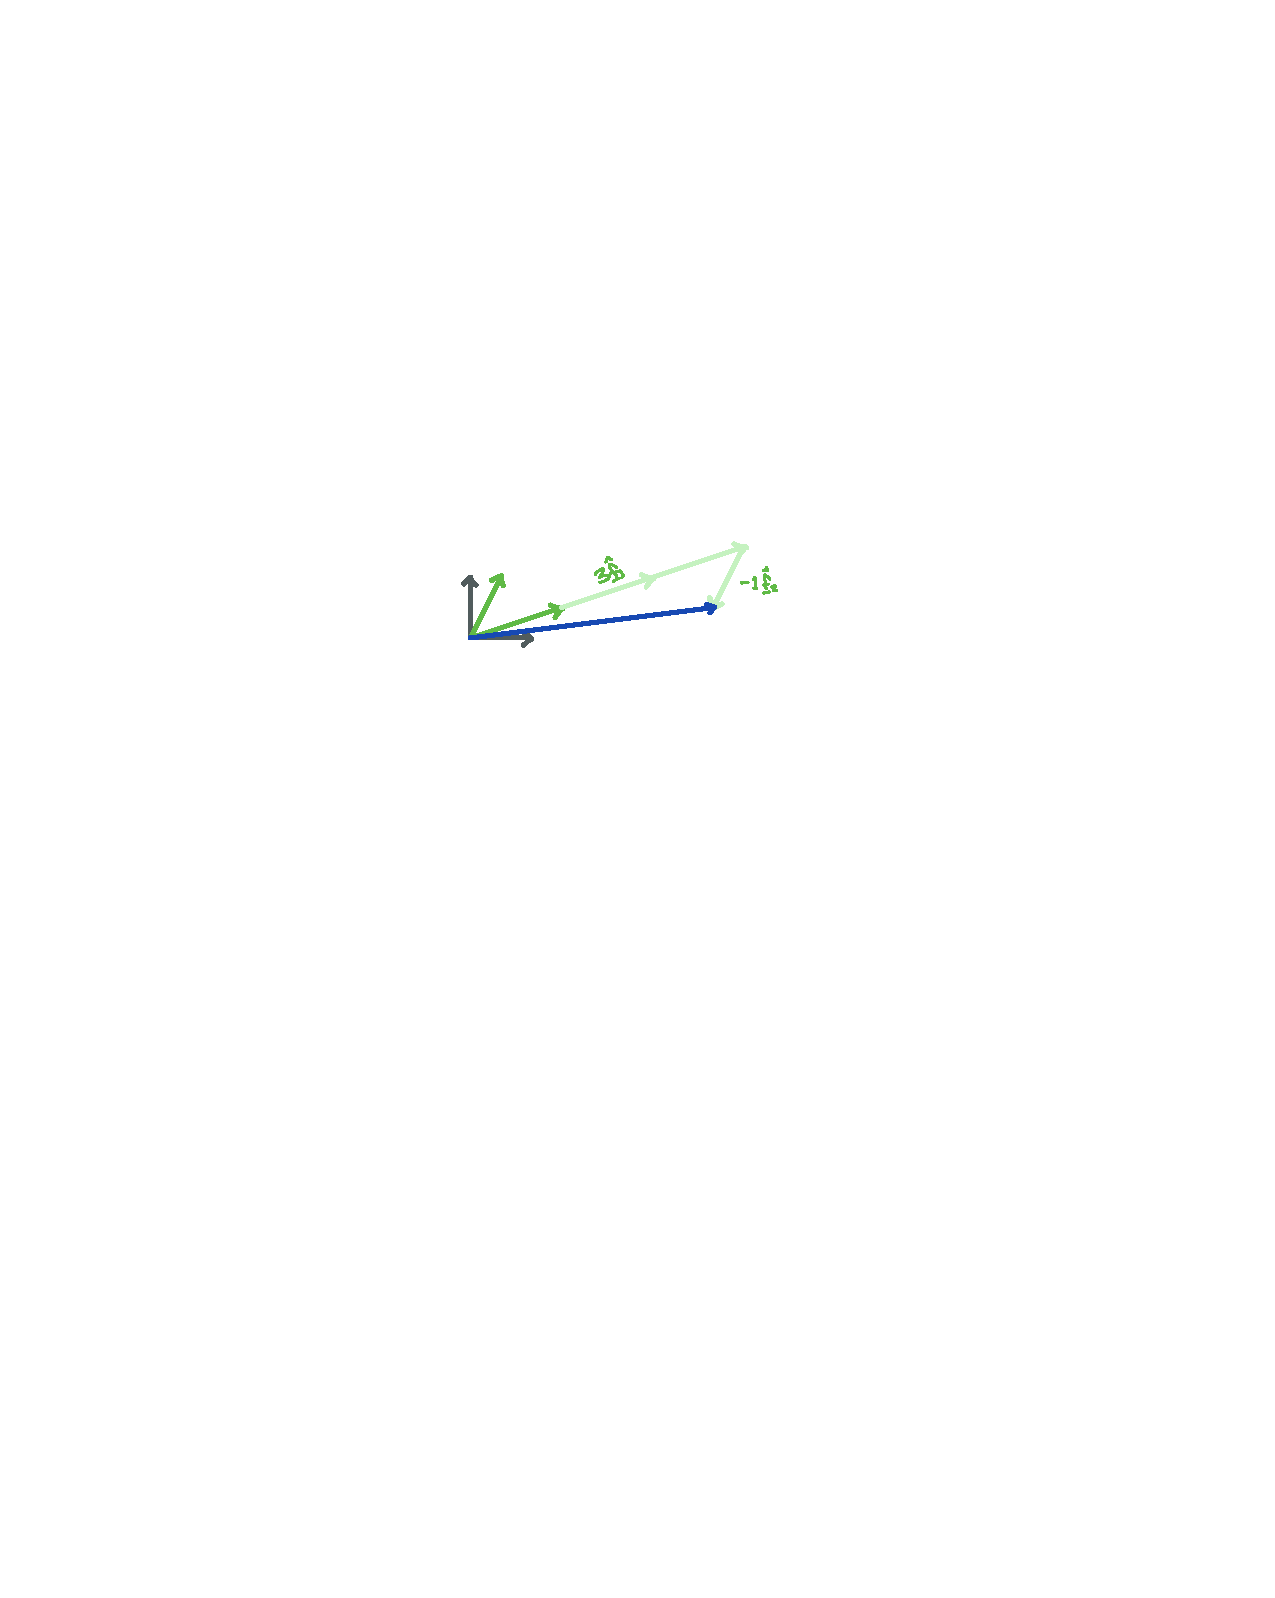
\includegraphics[width=\textwidth]{figures/basis_neg.pdf}
    \captionsetup{font={scriptsize,sf}}
    \caption{Example of a vector (blue) that has a negative coefficient of $\bas{f}_2$ in the $\bas{f}_{1,2}$ basis.}
    \label{fig:eg:basis:arrows:neg}
\end{marginfigure}

\begin{example}\label{ex:cheeseburger:space}
A silly vector space the space spanned by cheeseburgers ($\bas{e}_1$) and fries ($\bas{e}_2$) are your favorite local burger joint:
\begin{align}
\bas{e}_1 &=
    \eqfig{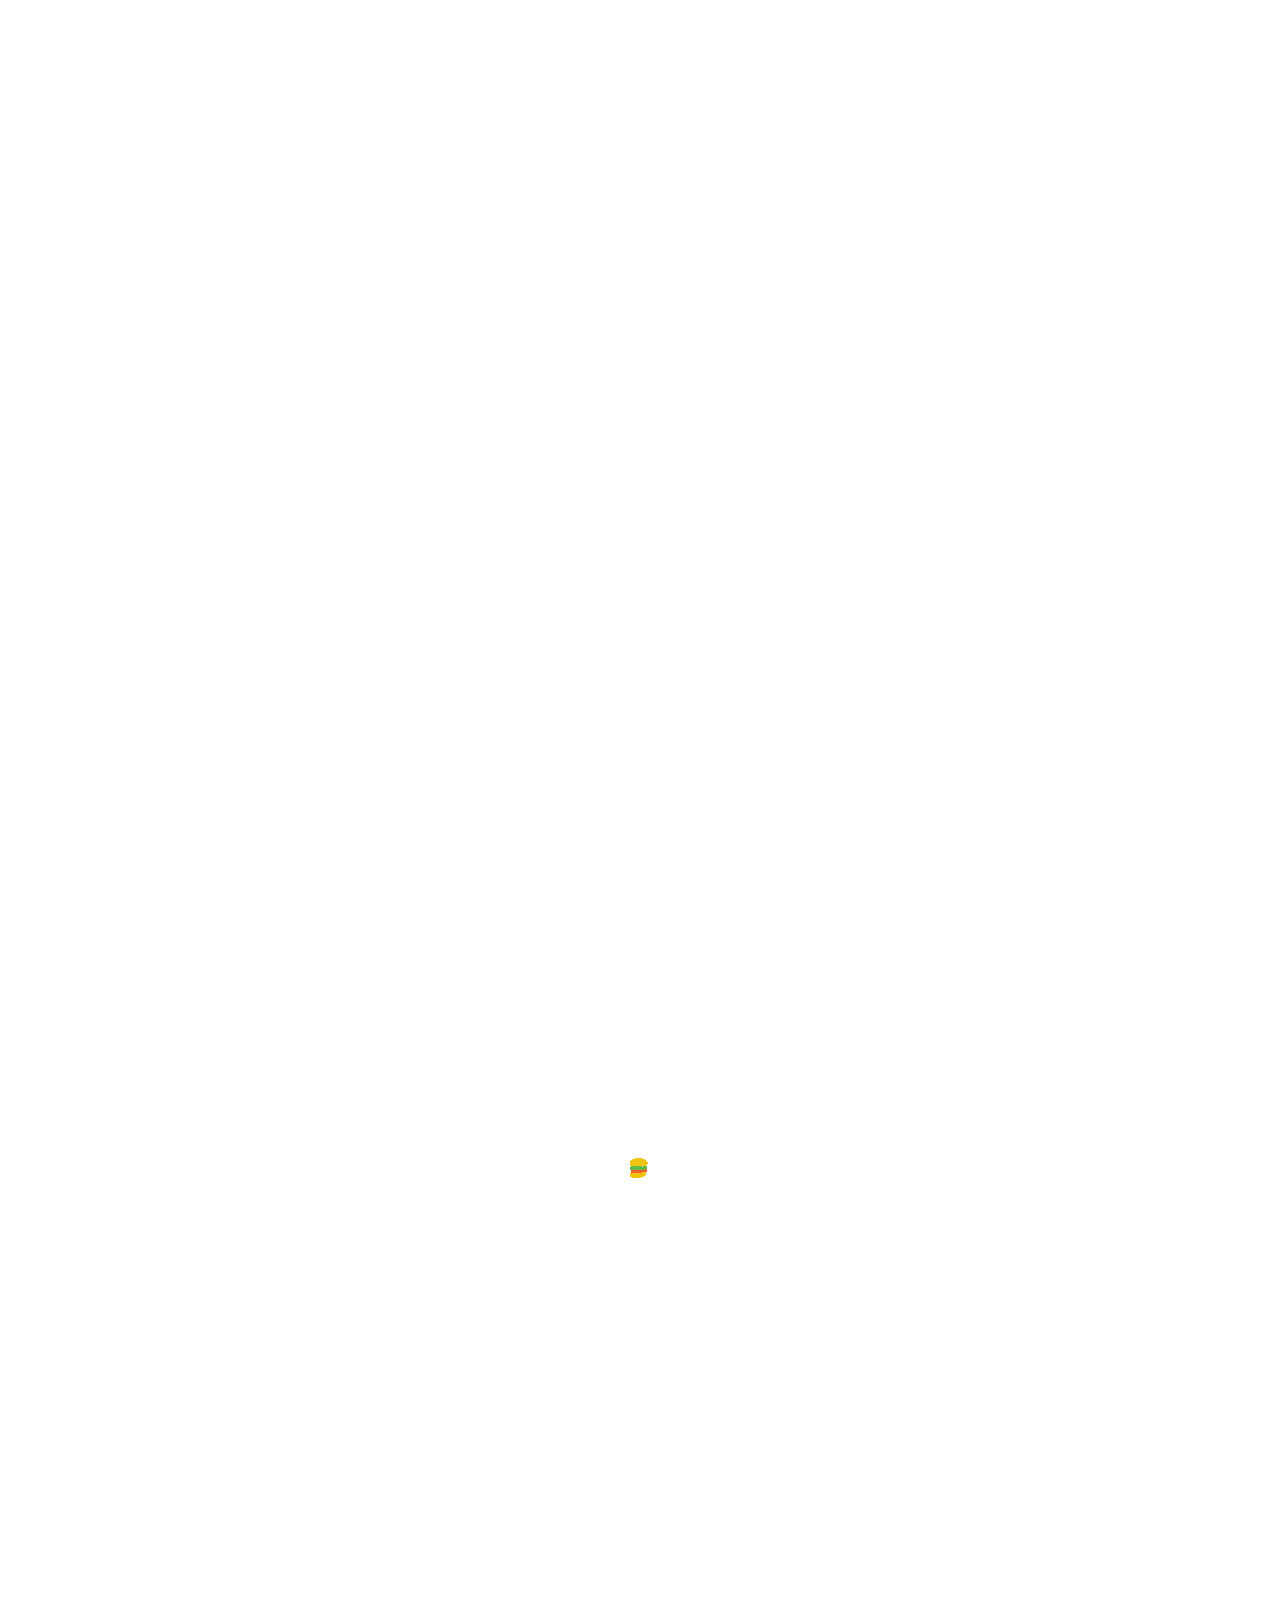
\includegraphics[width=1.5em]{figures/basis_food_icon_burger.pdf}}
    &
    \bas{e}_2 &=
    \eqfig{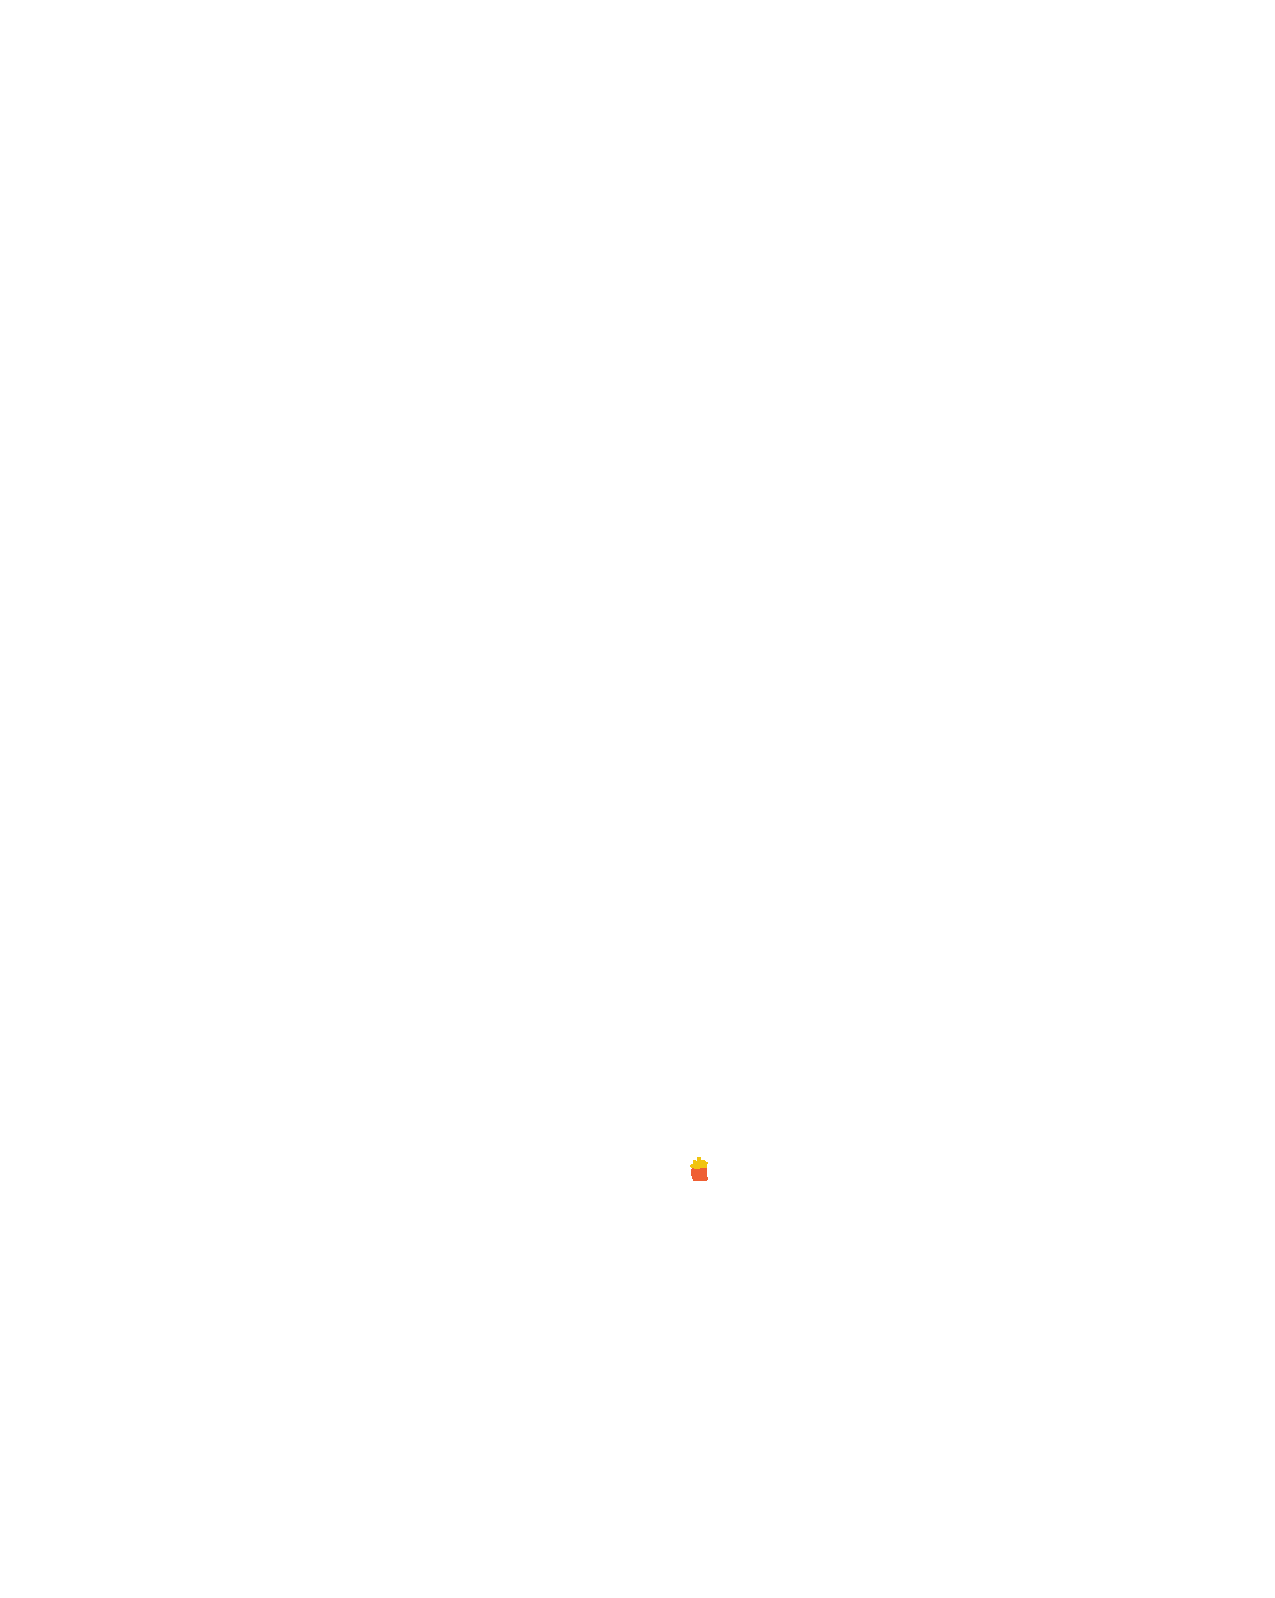
\includegraphics[width=1.5em]{figures/basis_food_icon_fries.pdf}} 
    &
    \eqfig{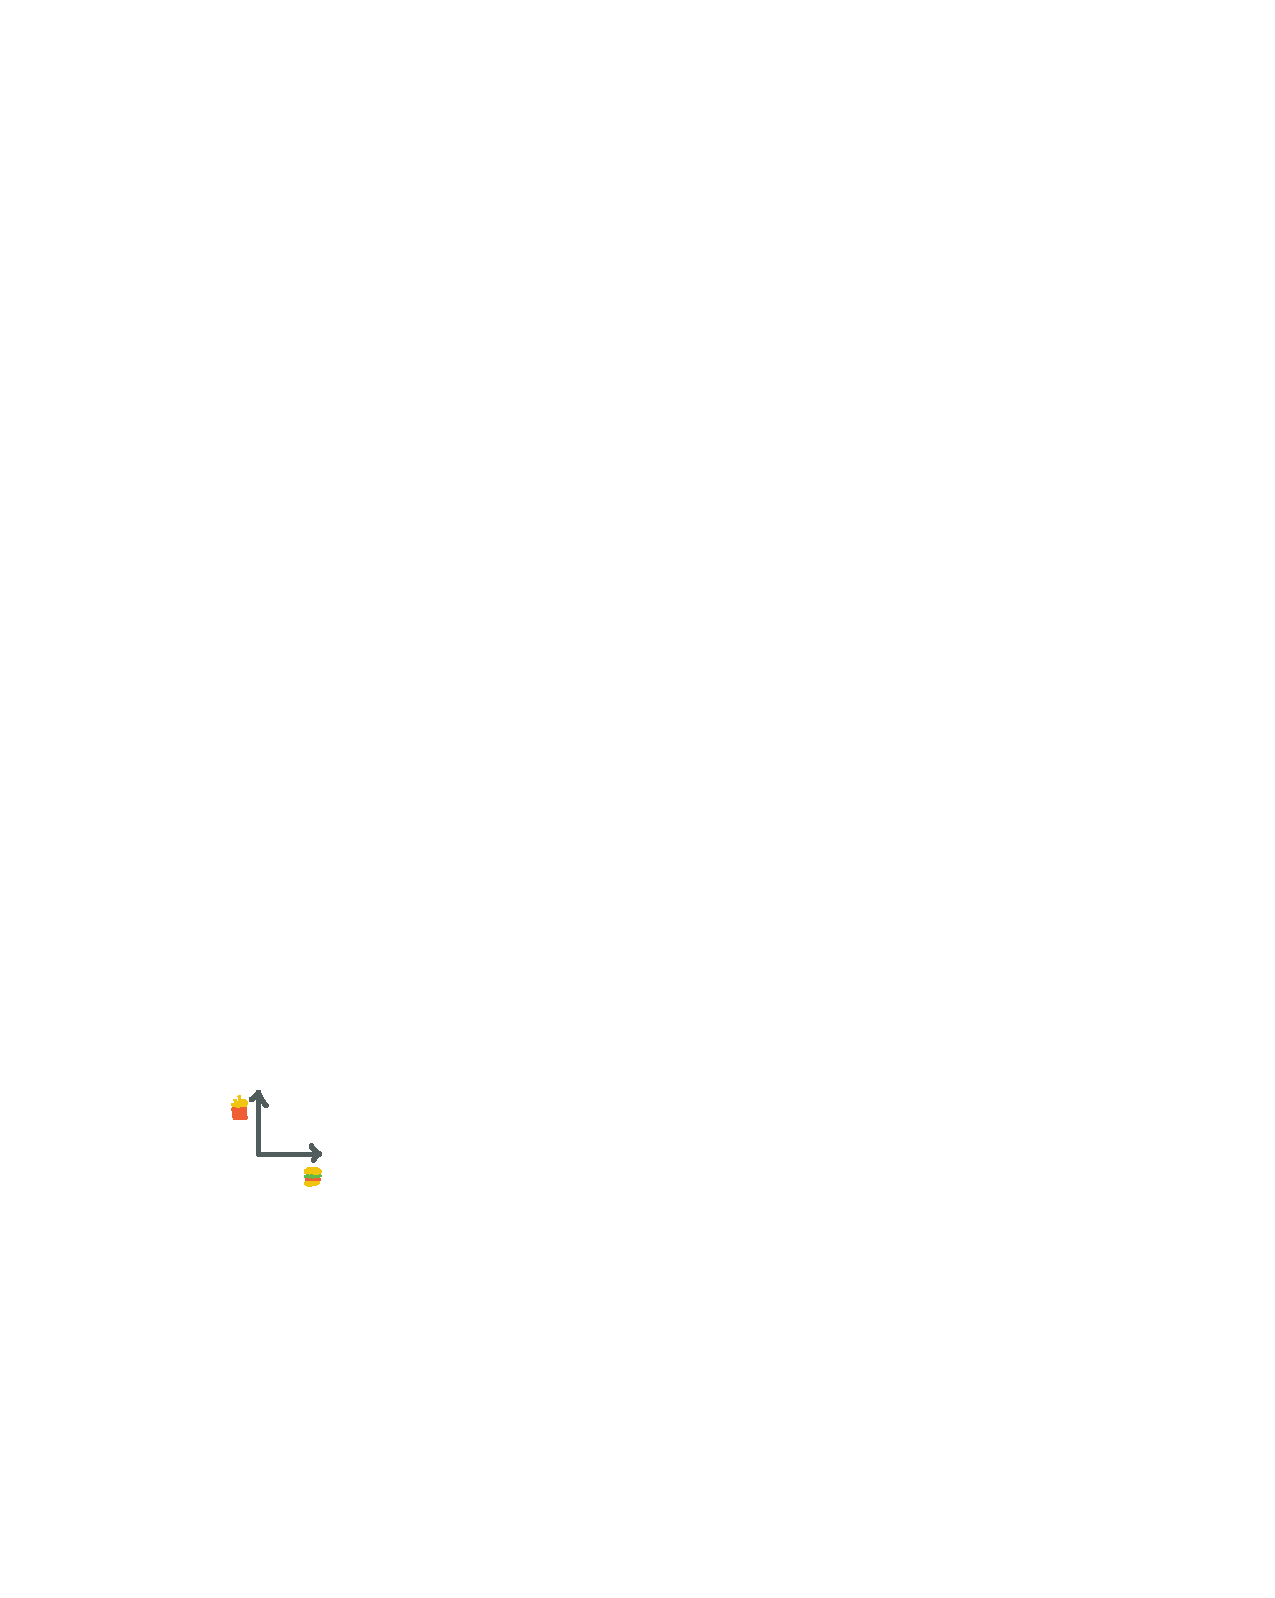
\includegraphics[width=4em]{figures/basis_food_canonical.pdf}} 
    \ .
\end{align}
Then an order $\vec{v}$ of 2 burgers and 1 fries is
\begin{align}
    \vec{v} =
    2\bas{e}_1 + \bas{e}_2 = 
    2\eqfig{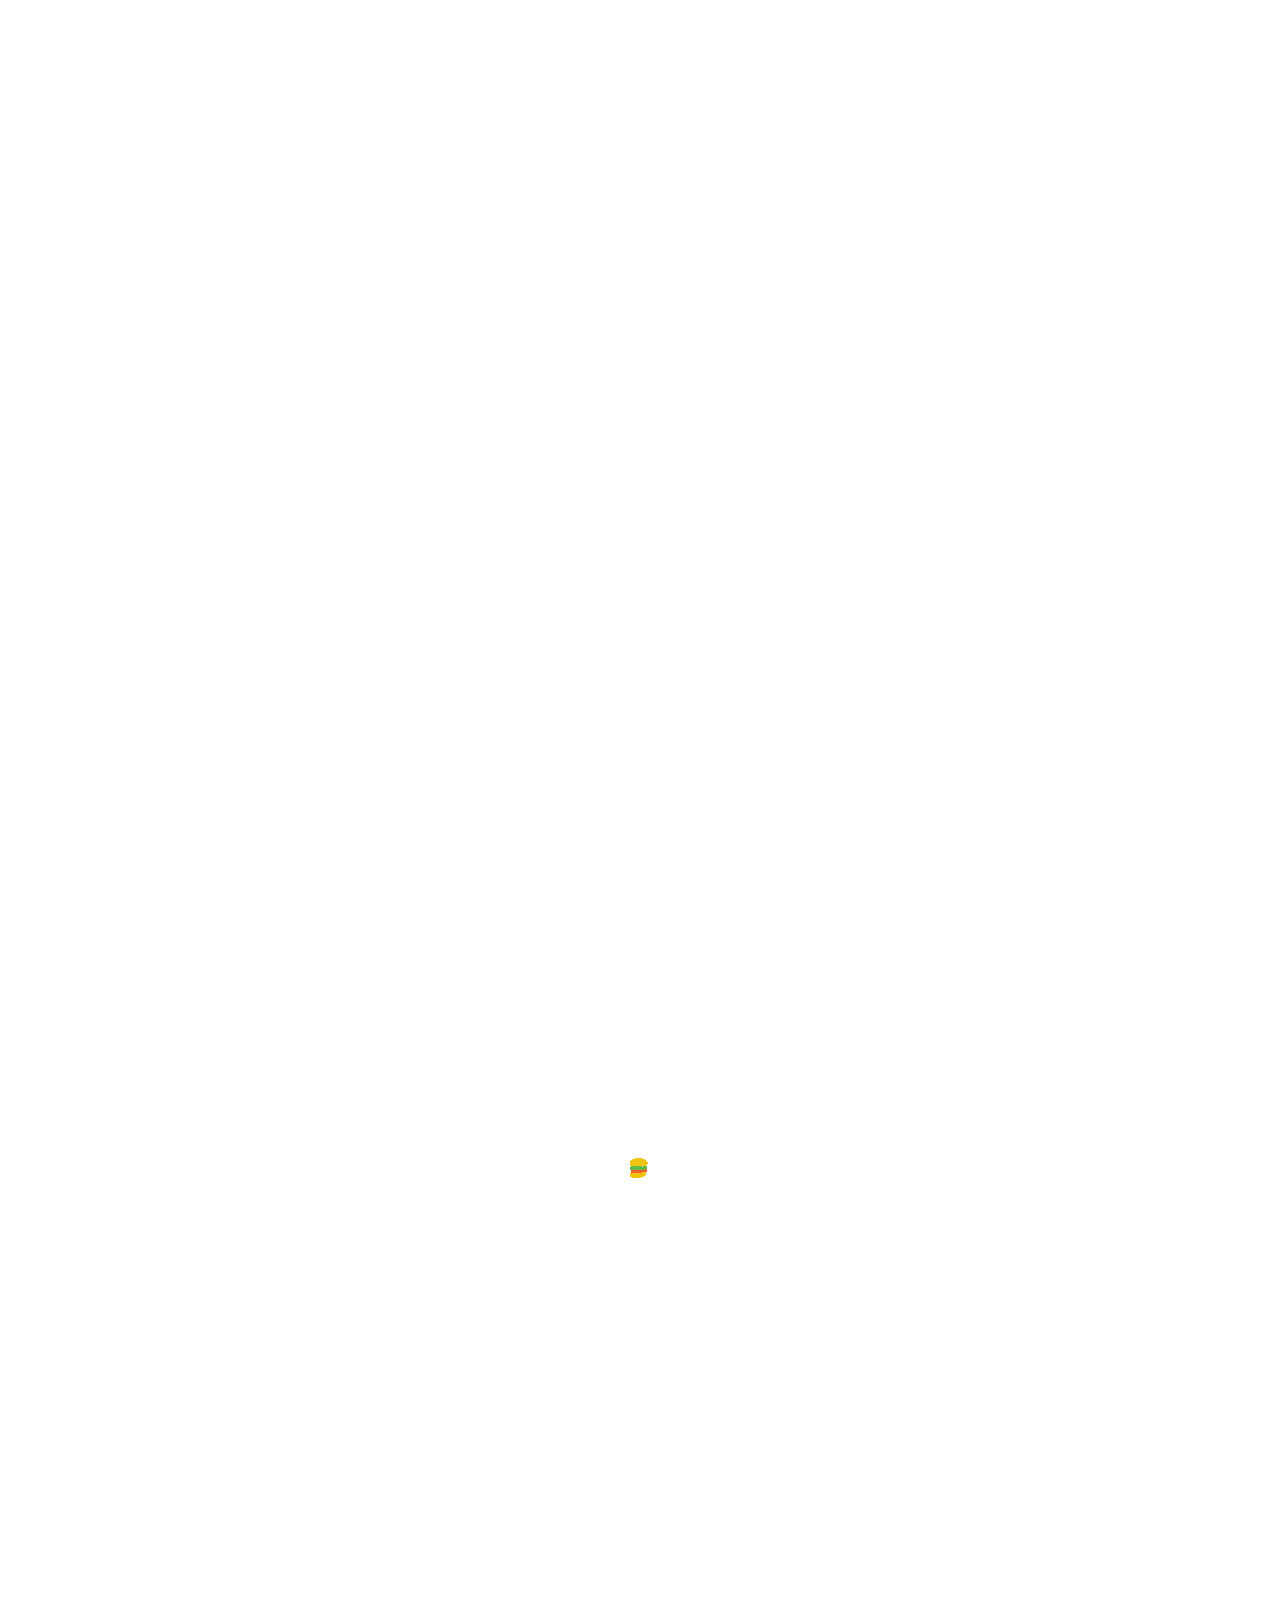
\includegraphics[width=1.5em]{figures/basis_food_icon_burger.pdf}} 
    +
    \eqfig{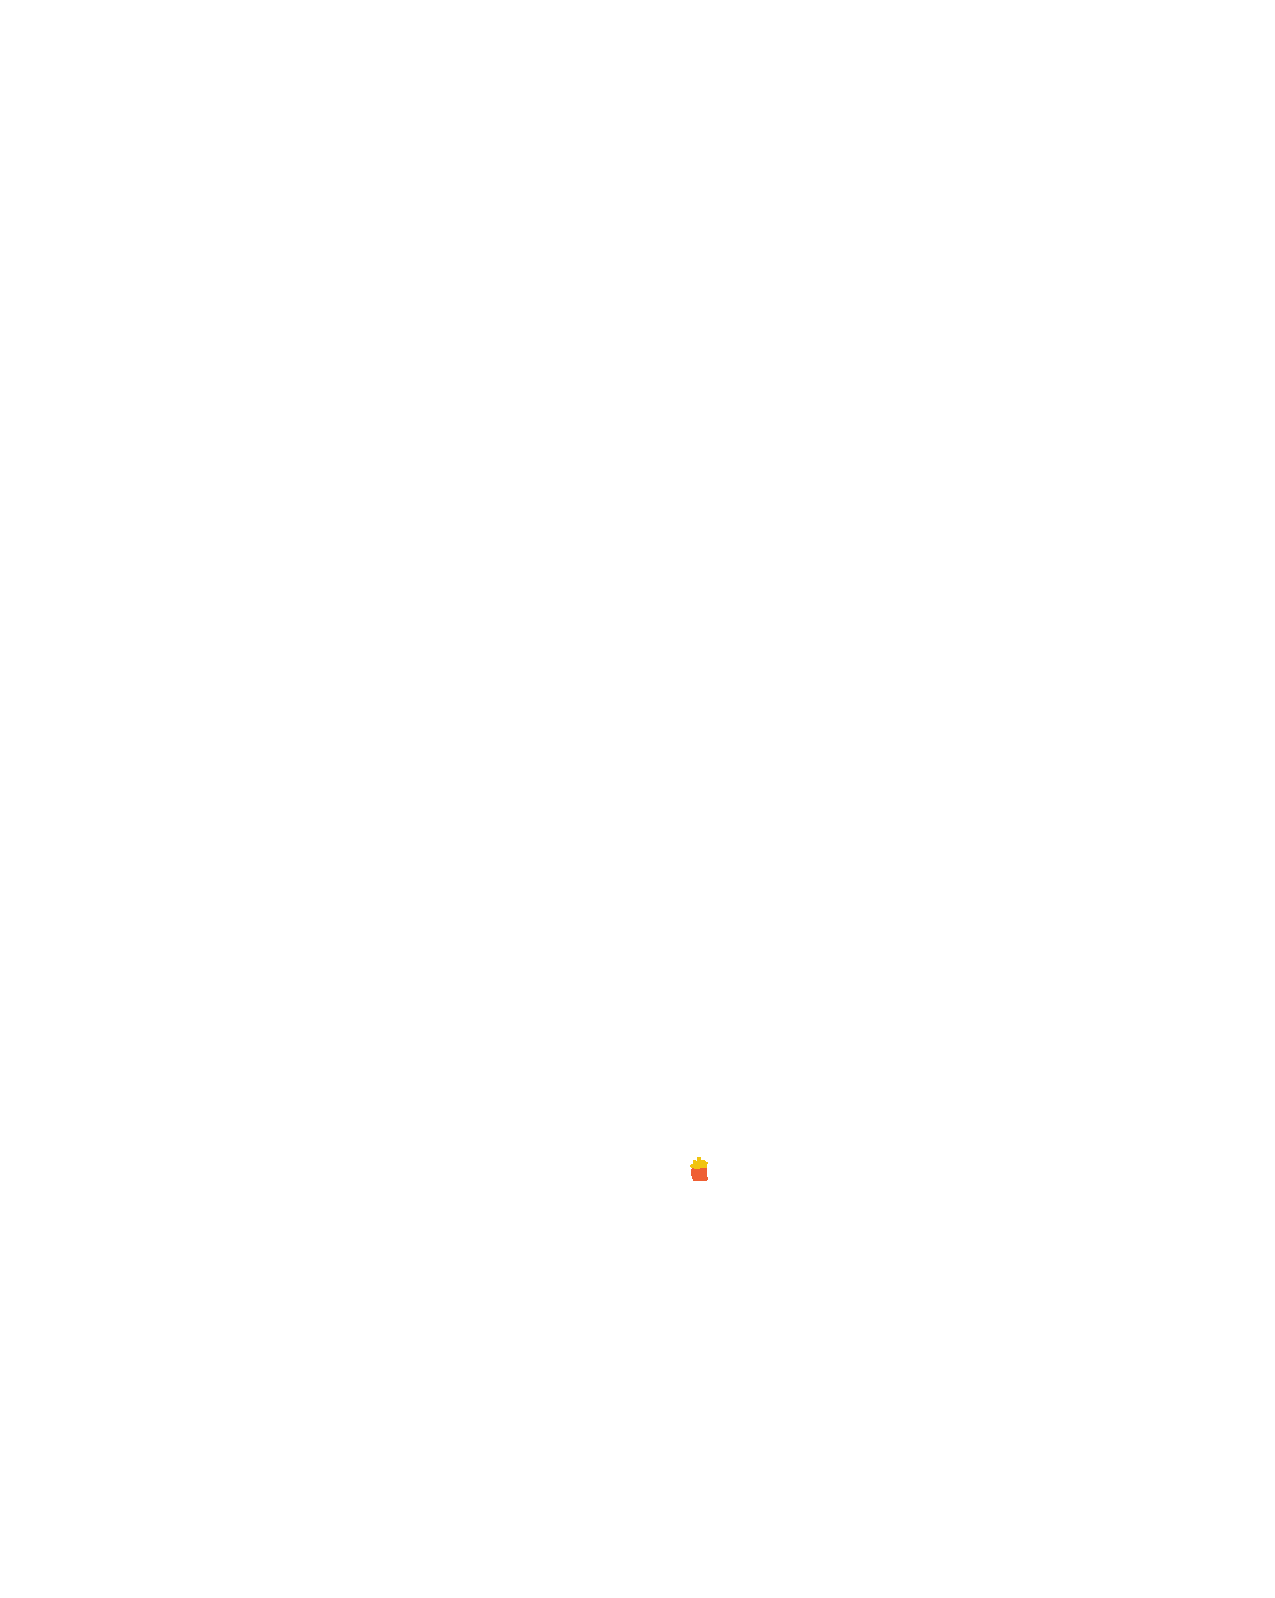
\includegraphics[width=1.5em]{figures/basis_food_icon_fries.pdf}} \ .
    \label{eq:basis:eg:meal:1}
\end{align}
Suppose the burger joint also offers a combo meal that includes one burger and one fries. Then we can choose another basis of combo meals ($\bas{f}_1$) and fries ($\bas{f}_2 = \bas{e}_2$); on the right we show it relative to the other basis:
\begin{align}
\bas{f}_1 &=
    \eqfig{
\includegraphics[width=1.5em]{figures/basis_food_icon_meal.pdf}}
    &
    \bas{f}_2 &=
    \eqfig{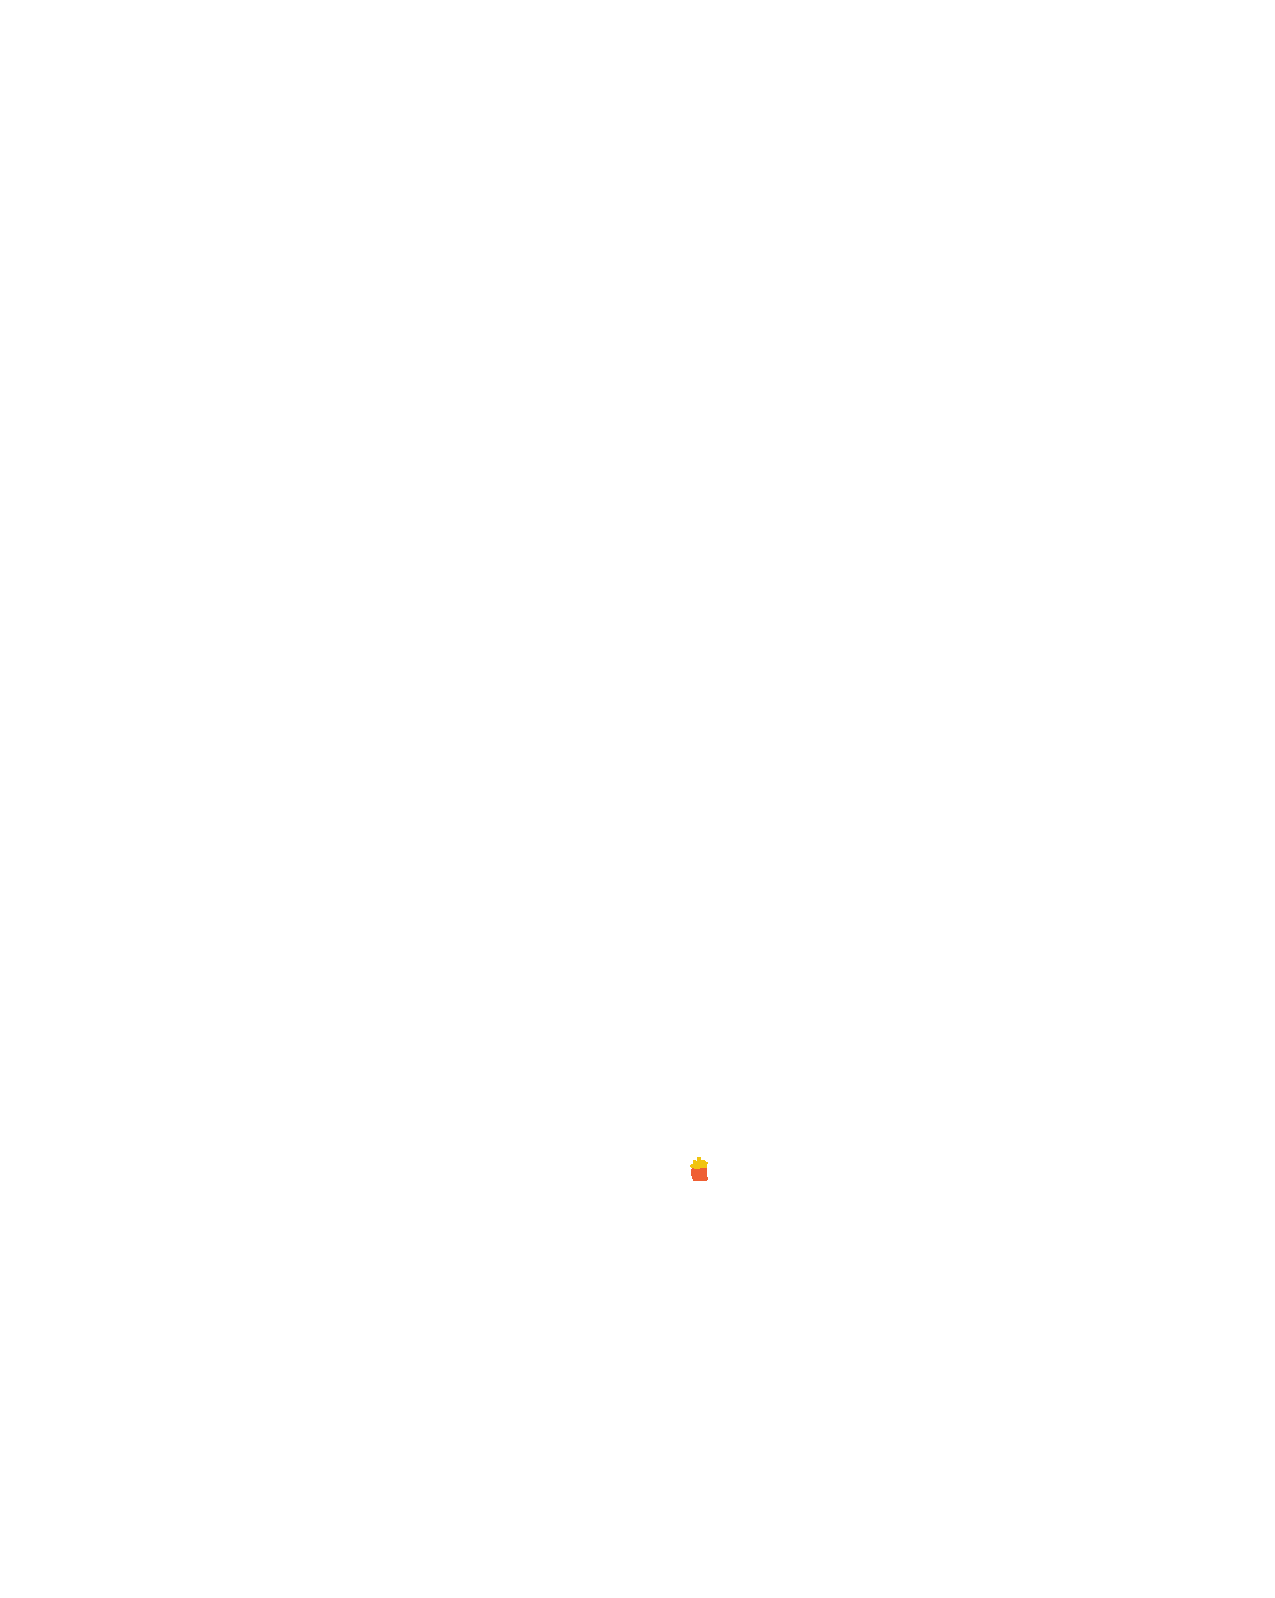
\includegraphics[width=1.5em]{figures/basis_food_icon_fries.pdf}} 
    &
    \eqfig{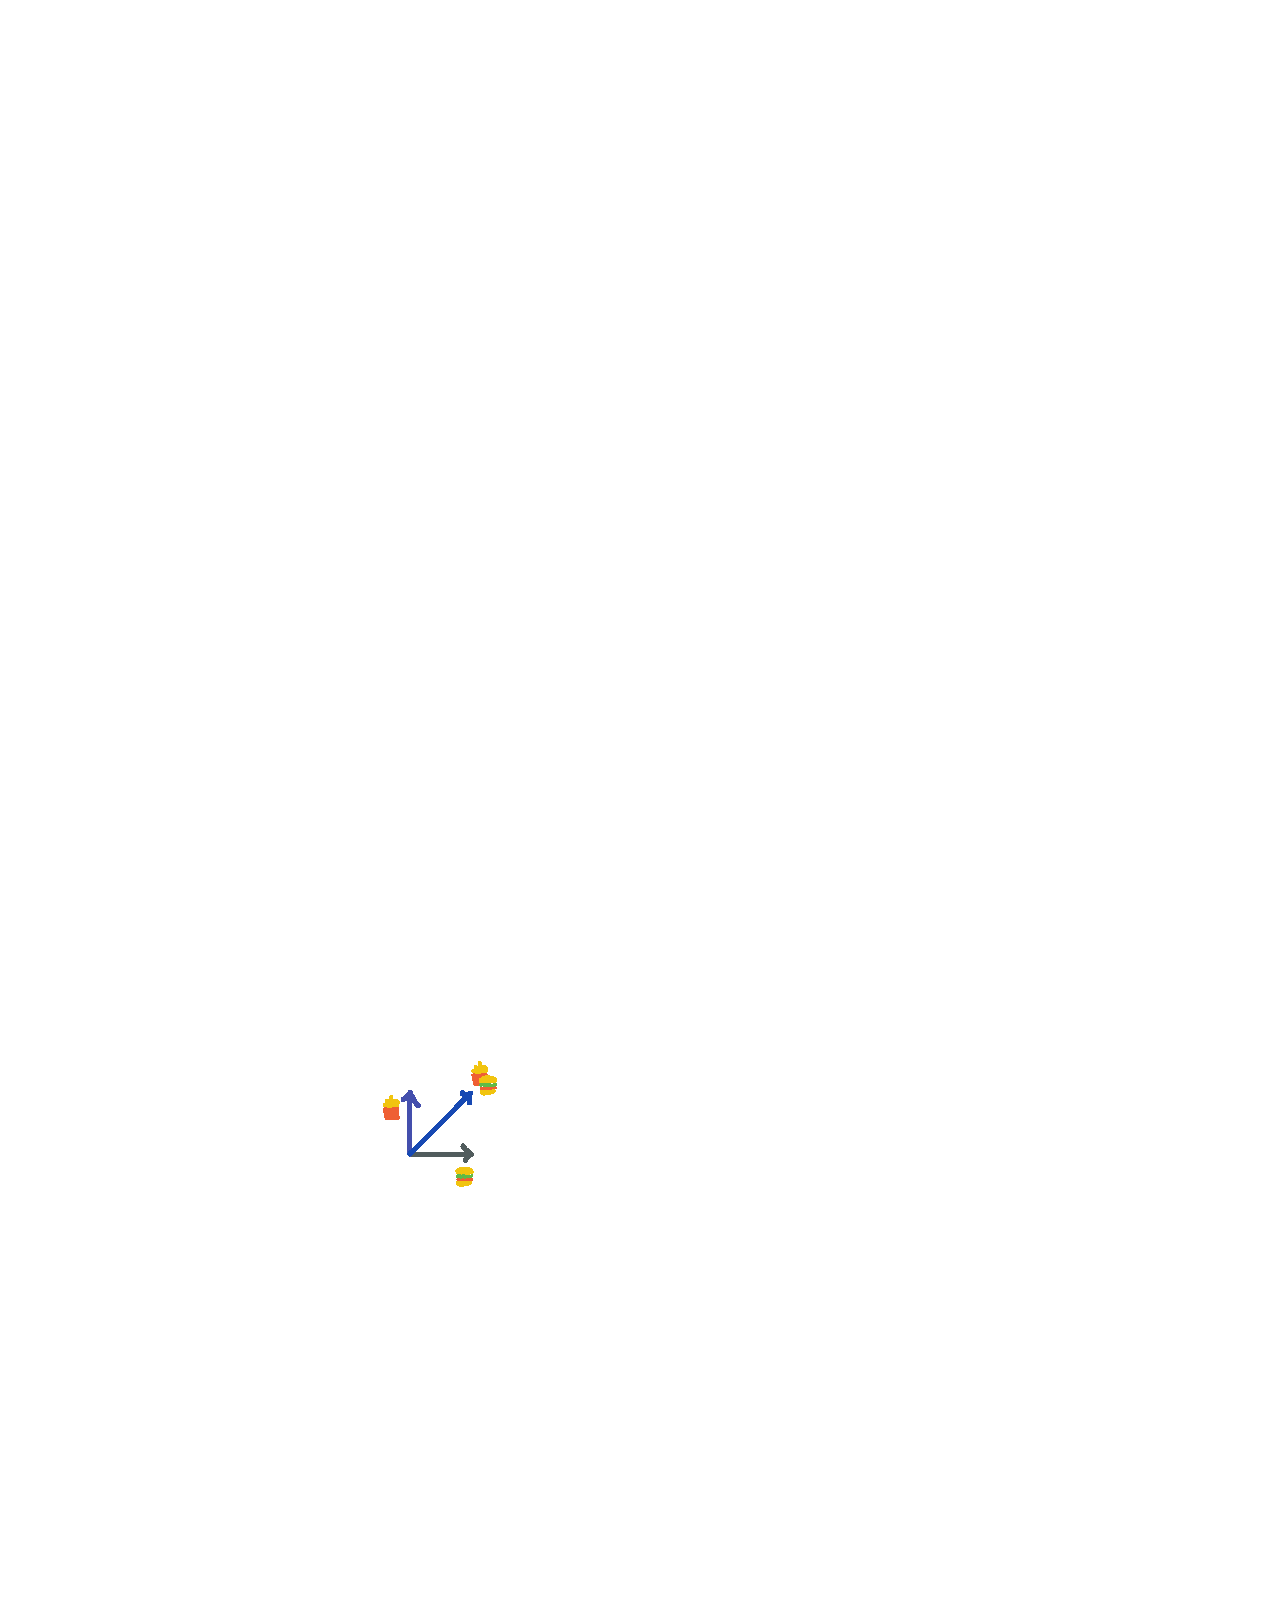
\includegraphics[width=5em]{figures/basis_food.pdf}} 
    \ .
\end{align}
Now an order $\vec{v}$ of two burgers and 1 fries is
\begin{align} 
    \vec{v} &=
    2\bas{f}_1 - \bas{f}_2 = 
    2\eqfig{
\includegraphics[width=1.5em]{figures/basis_food_icon_meal.pdf}}
    -
    \eqfig{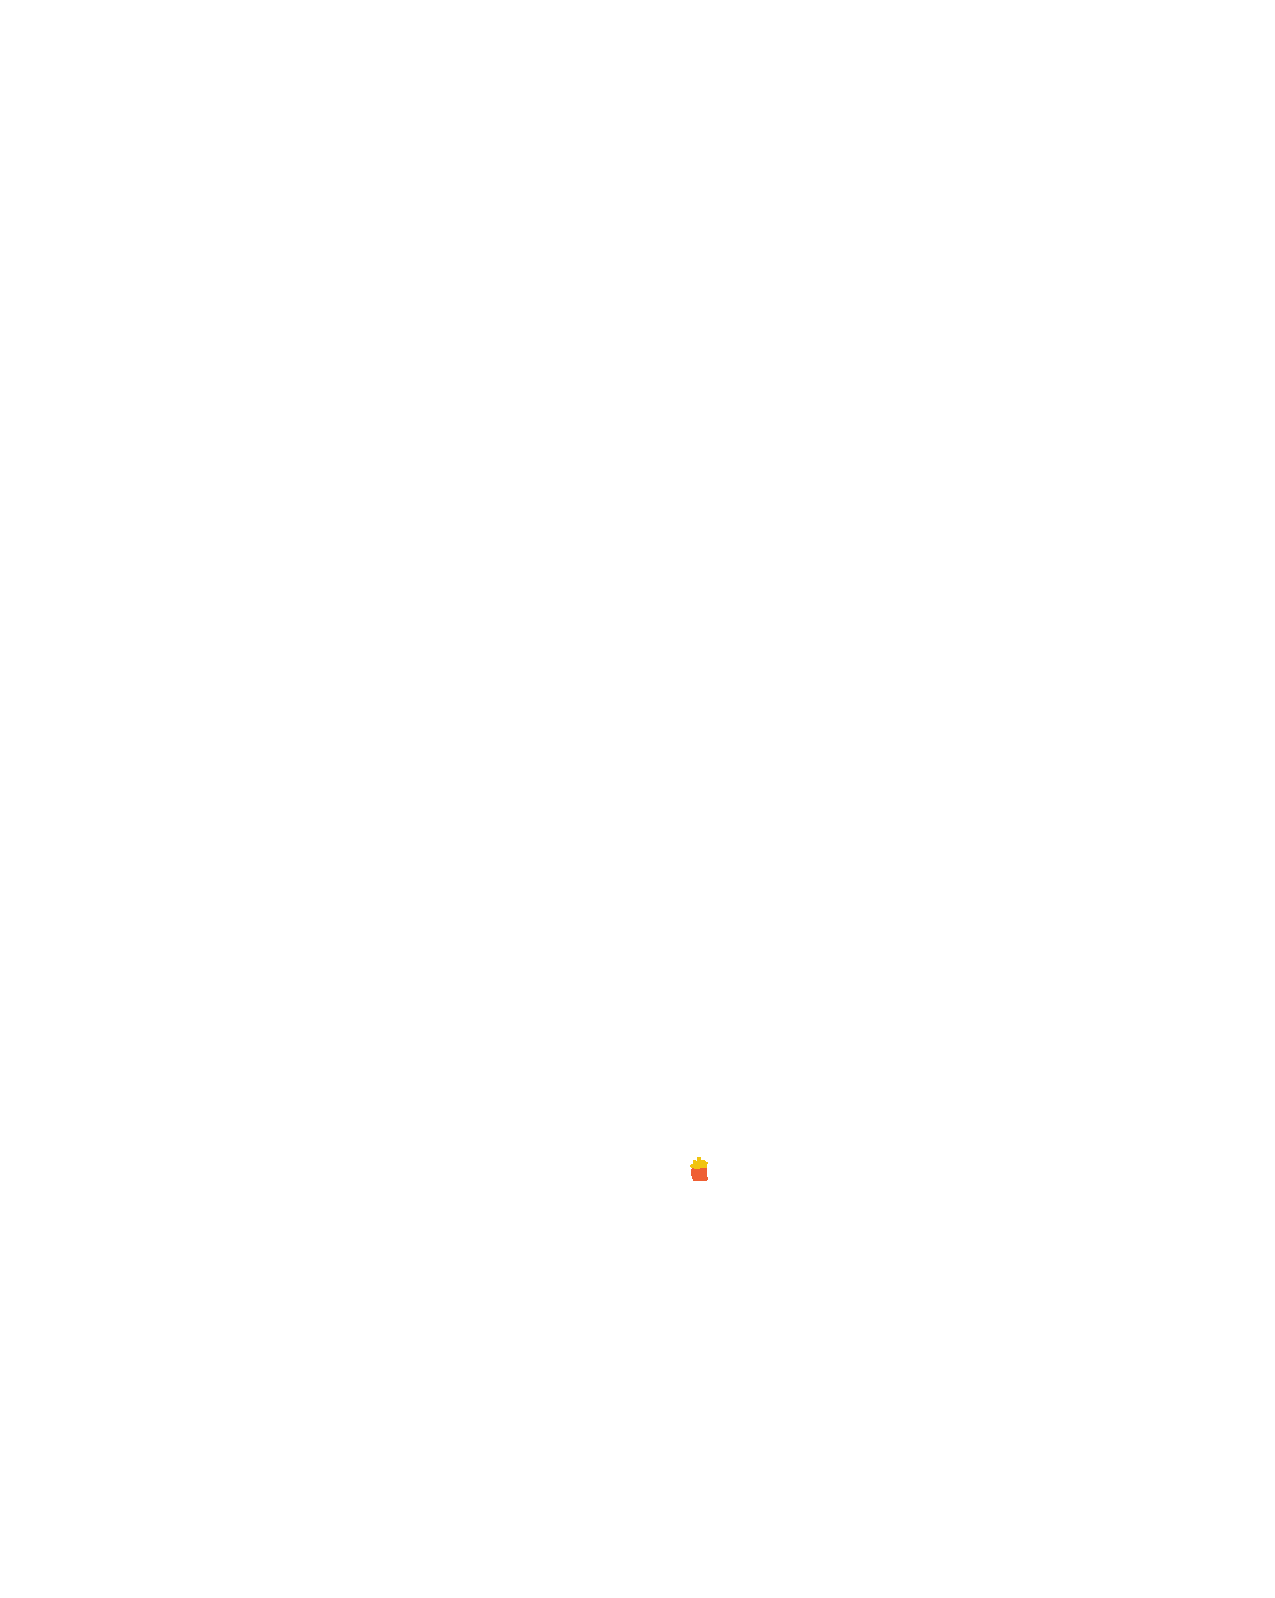
\includegraphics[width=1.5em]{figures/basis_food_icon_fries.pdf}} \ .
    \label{eq:basis:eg:meal:2}
\end{align}
We could also draw these as arrows. It would look something like this:
\begin{center}
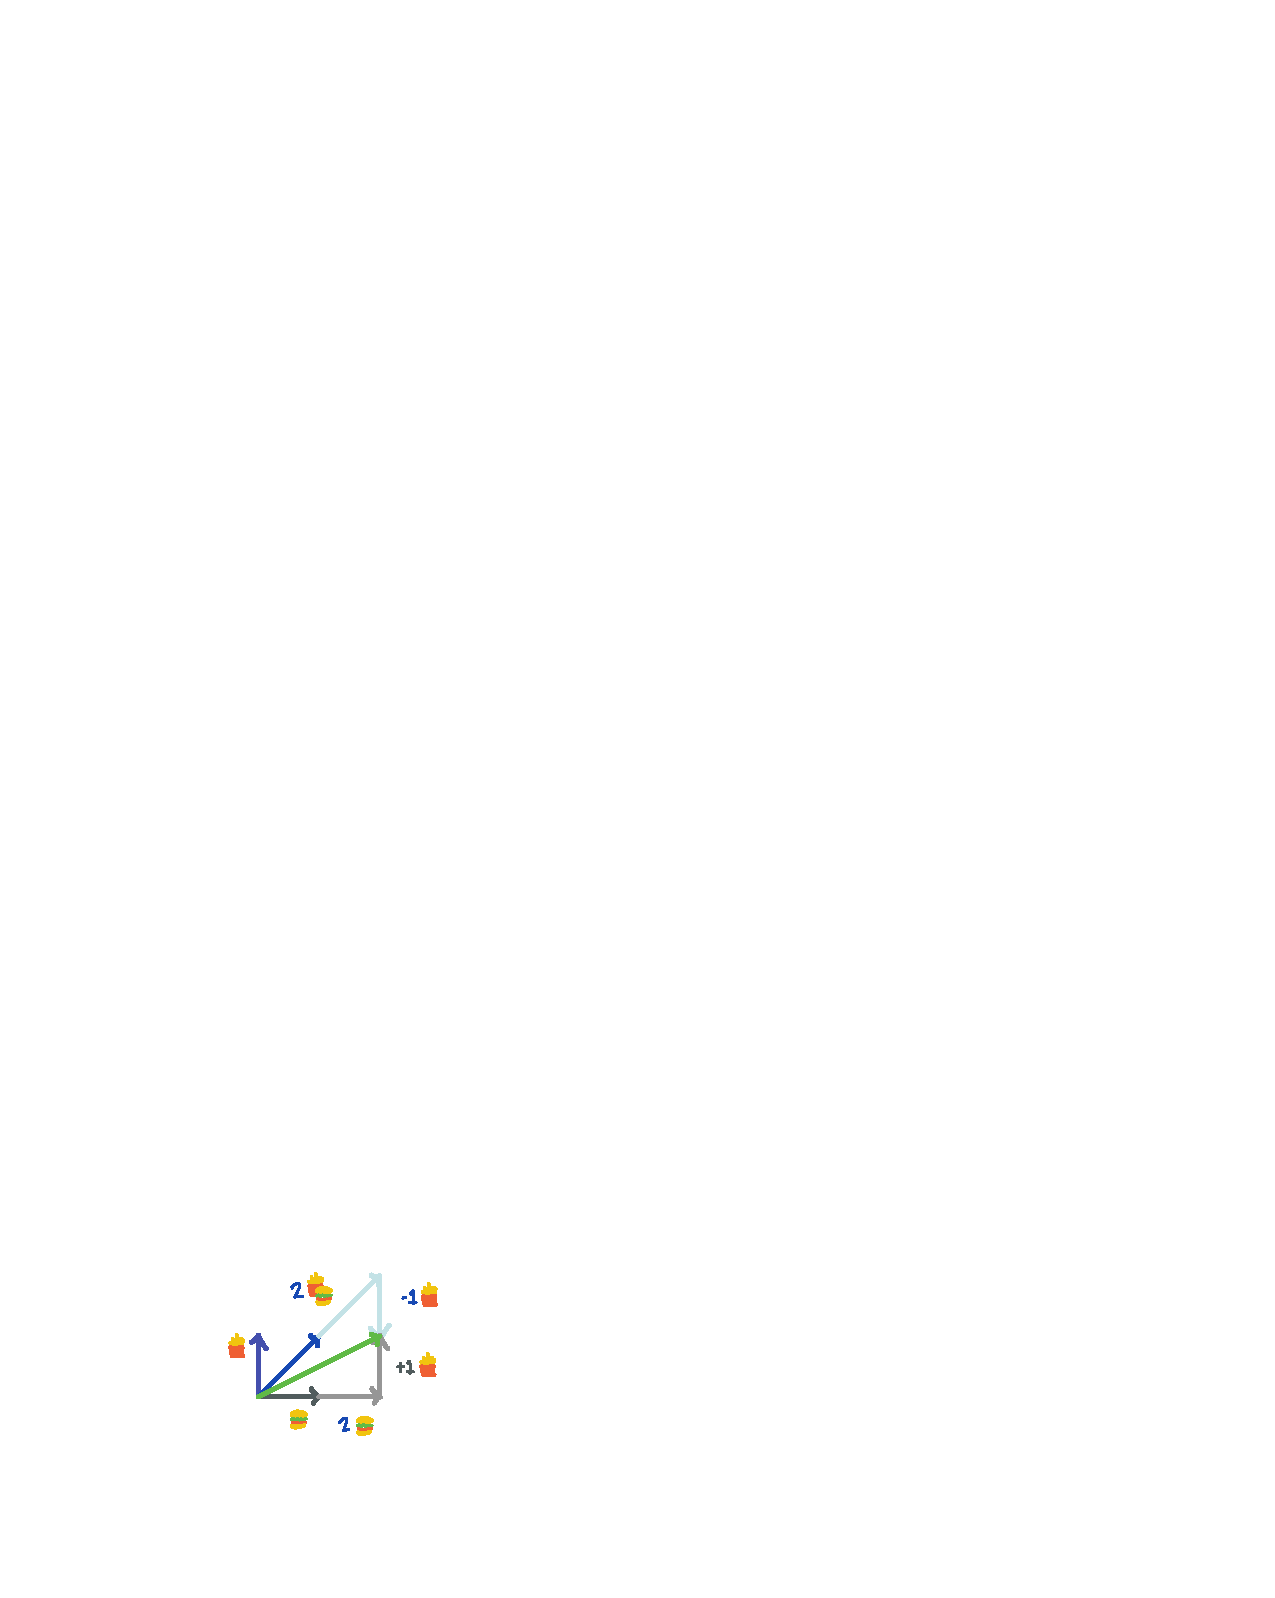
\includegraphics[width=.3\textwidth]{figures/basis_food_eg.pdf}
\end{center}
At this point, you could ask what a \emph{negative} order of fries ($-\bas{f}_2$) means. \emph{I don't know!} Maybe it means I should make fries for the cook? Maybe it means that fast food orders are not described well by vector spaces since the additive inverse may not have a clear meaning. But we have at least we are not talking about columns of numbers.
\end{example}


To make this concrete, please go through Exercise~\ref{ex:fibonacci:space} to meet a somewhat unusual vector space.
\begin{exercise}[Fibonacci sequence space]\label{ex:fibonacci:space}
One of my favorite examples of a vector space is the space of Fibonacci sequences. Fibonacci sequences are infinite lists of numbers $a_i$ that satisfy $a_{i+2} = a_i+a_{i+1}$. Once you specify the first two numbers $a_0$ and $a_1$, you can iteratively generate every other number in the sequence. Each sequence is a vector in the space of possible Fibonacci sequences. Show that this is true by confirming that a linear combination of Fibonacci sequences with each $i^\text{th}$ term added, e.g.\ $(a+b)^i = a_i+b_i$ is also a Fibonacci sequence. Give an example of a basis for the Fibonacci sequences. What is the dimension of the Fibonacci sequence space? \emph{Answer}: the dimension is two, even though each element is an infinitely long list of numbers.
\end{exercise}
\begin{marginfigure}%[th]
    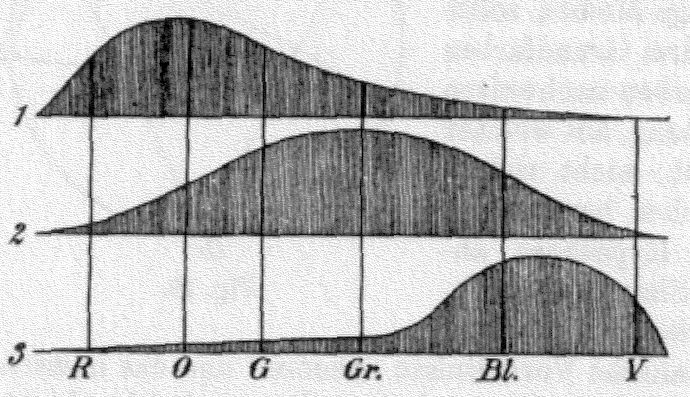
\includegraphics[width=\textwidth]{figures/YoungHelm.jpg}
    \captionsetup{font={scriptsize,sf}}
    \caption{Sketch of Young and Hemholtz (yes, the physicists) spectral sensitivities for different photoreceptors in their trichromatic color space theory. Image from Wikipedia, `Young-Hemholtz theory.'}
    \label{fig:young:hemholtz}
\end{marginfigure}
\begin{example}[Color space]\label{eg:color:space} is a vector space that highlights this idea of a more abstract basis vector. In color theory, all colors are linear combinations of red, green, and blue. This should sound really weird because in physics these colors are simply wavelengths of light: what is special about them? Nothing in nature. What is special is that our eyes have three types of color receptor cells, see Figure~\ref{fig:young:hemholtz}.\footnote{Animals can have different number of color receptor cells. One great place to read about this is Ed Yong's book, \emph{An Immense World}. Color space for those animals has a different dimension than ours.} Each type is sensitive to a certain window of the visible spectrum. We call these human eye responses the colors red, green, and blue. When we add colors, what we really mean is we're adding ``responses'' to a particular spectrum of light. When we add colors, we are not adding electromagnetic waves: we are adding neurological responses. For each type of color-sensitive cell, one `blip' of neural response is a basis vector for our color response. The sensation of a particular color is a linear combination of this basis. An actual human being is not sensitive to the whole vector space: for example, we cannot add negative colors to our sensory response. This is a fascinating subject and a surprising application of linear algebra.\footnote{There are some great YouTube videos on this. Here are a few: \url{https://www.youtube.com/watch?v=xAoljeRJ3lU}, \url{https://www.youtube.com/watch?v=AS1OHMW873s}, \url{https://www.youtube.com/watch?v=99v96TL-tuY}.} The sense in which a color is an overlap integral of a cell's sensitivity to different frequencies of light times the distribution of photons over frequency happens to also be a precursor to the inner product on infinite dimensional spaces.
\end{example}



\subsection{Changing basis} 
\label{sec:sub:basis:changing}

We started this section off by saying that the two of us just agreed on some set of basis vectors. Maybe we do not agree on a set of basis vectors. Maybe I am a little weird and I choose a set of basis vectors that seem very strange to you; this very strange basis does \emph{not} have to be aligned in any particular way.\sidenote{If you are about to say the word \emph{orthonormal}, then stop right there. We do not yet have the mathematical machinery to define orthogonality or normality.} 

\paragraph{A very silly basis}
Here is my silly choice of basis. To help us be very careful, I use square brackets for the components that \emph{you} would measure using \emph{your} basis. 
\begin{align}
    \bas{f}_1 &=
    \begin{bmatrix}
        3 \\ 1
    \end{bmatrix}
    &
    \bas{f}_2 &=
    \begin{bmatrix}
        2 \\ 2
    \end{bmatrix} \ .
\end{align}
All of my vectors are defined with respect to my basis. In fact, all the above line means is
\begin{align}
    \bas{f}_1 &= 3\bas{e}_1 + \bas{e}_2
    &
    \bas{f}_2 &= 2\bas{e}_2 + 2\bas{e}_2
    \ .
    \label{eq:change:basis:eg:1}
\end{align}
We can write this even more succinctly using tensors:
\begin{align}
    \bas{f}_i &= \bas{e}_j T\aij{j}{i} \ .
    \label{eq:change:basis:eg:2}
\end{align}
\begin{exercise}
What are the components of $T\aij{j}{i}$? \textsc{Partial answer:} $T\aij{1}{2} = 2$.
\end{exercise}


I can define a vector $\vec{a}$ with components $\alpha^{1,2}$ and package the components into a column with round brackets:
\begin{align}
    \vec{a} 
    = \begin{pmatrix}
        \alpha^1 \\ \alpha^2
    \end{pmatrix}
    =
    \alpha^i \bas{f}_i  \ .
\end{align}
What does this mean \emph{to you?} To figure this out, you would just insert the conversion \eqref{eq:change:basis:eg:1}:
\begin{align}
    \vec{a} = \alpha^i \bas{f}_i = \alpha^i T\aij{j}{i} \bas{e}_j = (\alpha^i T\aij{j}{i})\bas{e}_j \equiv \beta^j \bas{e}_j \ .
\end{align}
From this we find that the components of the vector $\vec{a}$ in your $\bas{e}_i$ basis are
\begin{align}
    \beta^j = \alpha^i T\aij{j}{i} \ . 
    \label{eq:beta:alpha:T:convert}
\end{align}
\begin{exercise}
Explicitly write out the $\beta^j$. \textsc{Partial answer:} $\beta^1 = 3\alpha^1 + 2\alpha^2$.
\end{exercise}


If I told you that I have a vector whose components---in my $\bas{f}$ basis---are
\begin{align}
    \alpha^1 &= 2 & \alpha^2 &= 3    
\end{align}
the you would understand that
\begin{align}
    \vec{a} 
    = \begin{pmatrix}
        \alpha^1 \\ \alpha^2
    \end{pmatrix}
    =
        \alpha^i \bas{f}_i 
        =
        2
    \begin{bmatrix}
        3 \\ 1
    \end{bmatrix}
    +
    3
    \begin{bmatrix}
        2 \\ 2
    \end{bmatrix}
    =
    \begin{bmatrix}
        12 \\
        8
    \end{bmatrix} 
    \equiv
    \begin{bmatrix}
        \beta^1 \\
        \beta^2
    \end{bmatrix}
    \ .
\end{align}
\begin{exercise}
Verify that these values of $\alpha^i$ and $\beta^i$ satisfy \eqref{eq:beta:alpha:T:convert}.
\end{exercise}
I am being \emph{very} careful here to distinguish between round and square brackets.
In tern, we must be \emph{very} careful in how we interpret this! The round brackets and the square brackets\sidenote{I just made up this notation for illustrative purposes.} are totally different objects. So the following statement is true:
\begin{align}
    \vec{a} = \begin{pmatrix}
        2 \\ 3
    \end{pmatrix}
    = 
    \begin{bmatrix}
        12 \\ 8
    \end{bmatrix} \ .
\end{align}
There is no paradox here: the column in round brackets are the components in the $\bas{f}$ basis while the column in square brackets are the components in the $\bas{e}$ basis. 


\paragraph{General discussion} The square and round bracket notation is somewhat cumbersome and non-standard. Instead, let us propose a notation that is just as cumbersome but more transparent:
\begin{align}
    \begin{pmatrix}
        \alpha^1\\
        \alpha^2\\
        \vdots
    \end{pmatrix}_{\bas{f}}
    &= \alpha^i \bas{f}_i
    &
    \begin{pmatrix}
        \beta^1\\
        \beta^2\\
        \vdots
    \end{pmatrix}_{\bas{e}}
    &= \beta^i \bas{e}_i \ .
\end{align}
A key idea is to see how we convert between bases.\sidenote{The plural of basis is \emph{bases} and is pronounced `bay-sees.' As a linguistic excursion, you can look up the plural of `hippopotamus.'}
\begin{align}
    \bas{f}_i = T\aij{j}{i} \bas{e}_j \ .
    \label{eq:change:of:basis:matrix:1}
\end{align}
We see that in the $\bas{e}$ basis,
\begin{align}
    \bas{f}_1 &=
    \begin{pmatrix}
        T\aij{1}{1}
        \\
        T\aij{2}{1}
        \\
        \vdots
    \end{pmatrix}_{\bas{e}}
\end{align}
and more generally,
\begin{align}
    \bas{f}_i &=
    \begin{pmatrix}
        T\aij{1}{i}
        \\
        T\aij{2}{i}
        \\
        \vdots
    \end{pmatrix}_{\bas{e}} \ .
\end{align}
And so we find the following rule.
\begin{newrule}[Change of basis matrix]\label{rule:change:of:basis:matrix}
Let $T\aij{i}{j}$ be the change of basis matrix defined by \eqref{eq:change:of:basis:matrix:1}. Then  the \emph{columns} of the matrix representation of $T\aij{i}{j}$ with the components of the $\bas{f}$ basis vectors written in the $\bas{e}$ basis:
\begin{align}
    \begin{pmatrix}
        T\aij{1}{1} & T\aij{1}{2} & \cdots \\
        T\aij{2}{1} & T\aij{2}{2} & \cdots \\
        \vdots & \vdots &\ddots  
    \end{pmatrix}
    &
    =
    \begin{pmatrix}
        | & | & \cdots \\
        \bas{f}_1 & \bas{f}_2 & \cdots \\
        | & | & \ddots 
    \end{pmatrix} \ .
\end{align}
\end{newrule}
Now let me take a moment to throw up swaths of caution tape here. The reason why the components of $\bas{f}_i$ in the $\bas{e}$ basis are given by the \emph{columns} of $T\aij{i}{j}$ has to do with our choice of how $T\aij{i}{j}$ is defined in \eqref{eq:change:of:basis:matrix:1}. In our strict index convention, \eqref{eq:change:of:basis:matrix:1} is the \emph{only} structure that makes sense.\sidenote{You could have defined a tensor $S_i^{\phantom{i}j}$ such that $\bas{f}_i = S_i^{\phantom{i}j} \bas{e}_j$, but we can equivalently define a matrix $T\aij{j}{i} = S_i^{\phantom{i}j}$ that does the same thing. If you are thinking about saying $S$ and $T$ transposes of each other---hold your horses! We do not yet have the machinery to define this.} 

We could then ask a separate question: if we know the components of a vector in the $\bas{e}$ basis, $\beta^i$, what are the components in the $\bas{f}$ basis? Then we can take \eqref{eq:change:of:basis:matrix:1} and act on both sides with the inverse transformation $(T\inv)\aij{i}{k}$
\begin{align}
    (T\inv)\aij{i}{k}T\aij{j}{i}\bas{e}_j &= (T\inv)\aij{i}{k}\bas{f}_i \\
    \delta^j_k \bas{e}_j &= (T\inv)\aij{i}{k}\bas{f}_i\\
    \bas{e}_k &=(T\inv)\aij{i}{k}\bas{f}_i \ ,
    \label{eq:intermediate:e:Tinv:f}
\end{align}
Where we use the Kronecker-$\delta$ from \eqref{eq:kronecker:delta}.
% 
Contracting both sides \eqref{eq:intermediate:e:Tinv:f} by the $\bas{e}$ basis components $\beta^k$ then gives an expression for the $\alpha^k$ components in the $\bas{f}$ basis:
\begin{align}
   \beta^k \bas{e}_k &=(T\inv)\aij{i}{k} \beta^k \bas{f}_i \equiv \alpha^i \bas{f}_i \ .
\end{align}
In other words,
\begin{align}
    \alpha^i = (T\inv)\aij{i}{k} \beta^k \ .
\end{align}
Of course, at this point you can wonder about what to do if $T$ is \emph{not} an invertible matrix---and under what conditions would that be the case? Evidently we should put some thought into what a `good' basis might be, and part of that definition is likely to involve the invertibility of the transformation between different `good' bases.

\begin{bigidea}\label{idea:2d:chart}
In physics, a choice of basis often corresponds to a reference frame. For example, we could imagine trying to look at a paper map\footnote{In ancient times maps used to be printed on large pieces of paper that were folded up. Ancient navigators would find shared community in trying to re-fold these maps so that they might fit back into their glove compartments.} while standing in Parking Lot 13 at \acro{UC R}iverside. There is a two dimensional vector space of directions from where we are standing. A natural basis is 
\begin{align}
    \bas{e}_1 &= \text{step forward}\\
    \bas{e}_2 &= \text{step to the right} \ .
\end{align}
Taking a two steps to the left would be $-2\bas{e}_2$. Then I could use my map and tell you that the Physics department is located\footnote{Nevermind that `position vectors' are not a sensible thing. As an exercise, you can try to rephrase this example in terms of velocities. It gets clunky: you are trying to throw a football with some velocity so that it reaches the physics department in a certain fixed amount of time. Analogies are like undergrads... \url{https://phdcomics.com/comics/archive.php?comicid=439}} at $900\bas{e}_1$. This is only correct if my $\bas{e}_1$ basis vector is pointing east; that is, if I am facing east. If you happen to be facing north-east, then your basis vectors would be oriented differently. Perhaps $\bas{f}_1$ still means a `step forward,' but now it is a step in the north-east direction.

We want to be able to describe physical situations in different orientations. It is often easier to describe a problem in a different frame. For example, the frame where the angular momentum (pseudo-)vector is pointed in the $z$ direction, or where the moment of inertia tensor is diagonal. In relativity, it is usually helpful to be able to boost to the rest frame of a moving body.

A more sophisticated version of a change of basis is the description of a quantum particle using its position versus its momentum. Some problems are much easier to solve if you describe the particle in terms of its momentum, while others are easier if you use position. One of the curiosities of quantum mechanics is that these two descriptions turn out to be incompatible, as manifested in the Heisenberg uncertainty relations.

All this is to say that yes: changing basis is a big $\bas{f}$'ing deal.\footnote{To paraphrase a former vice president.}
\end{bigidea}



\subsection{Goldilocks dimension} % Why isn't the modern telling called ``Karen and the three bears?''

Recall from \eqref{eq:linear:combination:looks:like:basis} that the span of a set of vectors $\vec{v}_1, \cdots, \vec{v}_N$ is the vector space $V$ of all linear combinations of those vectors. This makes us want to identify those vectors as a basis for $V$. \emph{Not so fast}. For any vector space $V$, there is a `correct' number of basis vectors vectors called the \textbf{dimension}\index{dimension} of $V$, or $\text{dim}\,V$. This dimension is the minimum number of good basis vectors that you need to describe any vector in $V$. To write it technically, $\text{dim}\,V$ is the smallest counting number $d$ such that
\begin{align}
    \forall \vec{v} \in V :\; \vec{v} = v^1 \bas{e}_1 + \cdots + v^{d}\bas{e}_{d} \ .
\end{align}
The symbol $\forall$ means ``for all,'' so the above line says: for all (really: for \emph{any}) vector $\vec{v}$ in the vector space, $\vec{v}$ is a linear combination of $d$ basis vectors. The dimension of $V$ is the smallest number $d$ for which this is true. 

If your number of proposed basis vectors is larger than this dimension then vectors do not have a unique expansion. If your number of proposed basis vectors is smaller than this dimension, then there are vectors in $V$ that \emph{cannot} be described by linear combinations of your basis vectors. And even if your number of proposed basis vectors is \emph{just right} and exactly equal to $\text{dim}\,V$, you could \emph{still} fail because some of your basis vectors are actually combinations of other basis vectors. Let us go through these cases sequentially.

\subsubsection{Too many basis vectors}

Start with the following example:
\begin{example}
Suppose you have the following proposed basis:
\begin{align}
    \bas{e}_1 &=
    \begin{pmatrix}
        1\\
        1
    \end{pmatrix}
    &
    \bas{e}_2 &=
    \begin{pmatrix}
        2\\
        1
    \end{pmatrix}
    &
    \bas{e}_3 &=
    \begin{pmatrix}
        -1\\
        \pp 1
    \end{pmatrix} \ .
    \label{eq:eg:too:many:basis:vectors:basis}
\end{align}
Suppose I then give you the vector
\begin{align}
    \vec{v} &=
    \begin{pmatrix}
        3 \\ 1
    \end{pmatrix} \ .
\end{align}
What is the linear combination of your basis vectors that produces $\vec{v}$? In other words, what are the $v^i$ so that
\begin{align}
    \vec{v}= v^i \bas{e}_i \, ?
\end{align}
You can write this as a system of equations. One solution is
\begin{align}
    \vec{v} &= -1\bas{e}_1 + 3\bas{e}_2 + 0\,\bas{e}_3 
    &
    \begin{pmatrix}
        v^1 \\ v^2 \\ v^3
    \end{pmatrix}
    =
    \begin{pmatrix}
        -1 \\ \pp 3 \\ \pp 0
    \end{pmatrix} \ .
\end{align}
Great, problem solved, right? Not quite. We could have \emph{alternatively} written
\begin{align}
    \vec{v} &= 0\,\bas{e}_1 + \frac{4}{3}\bas{e}_2 - \frac{1}{3}\bas{e}_3 
    &
    \begin{pmatrix}
        v^1 \\ v^2 \\ v^3
    \end{pmatrix}
    =
    \begin{pmatrix}
        \pp 0 \\ \pp 4/3 \\ - 1/3
    \end{pmatrix} \ .
\end{align}
Now we should be concerned. For the \emph{same} basis, there are at least \emph{two} different sets of coefficients that describe the \emph{same} vector! How are we supposed to keep track of the fact that there are \emph{degeneracies} where different combinations of components $v^i$ actually mean the \emph{same} vector? That would be madness.\sidenotemark
\end{example}\sidenotetext{This is absolutely silly to do, but it turns out there are cases in physics where we make use of this type of madness. These are called \emph{gauge theories}. An example of a gauge theory is electromagnetism, where there is a redundancy that we call a \emph{gauge symmetry}. This corresponds to the fact that many different choices of gauge potential (the electric and vector potentials) produce the same physical electric and magnetic fields. An excellent introduction to this idea is \arXiv{hep-th/0611201}.}
\begin{exercise}
Write out and solve the system of equations from the previous example. Show that there are an infinite number of solutions. In fact, these solutions are a line in a three-dimensional space.
\end{exercise}

Evidently you can have \emph{too many} basis vectors. In the above example, we could have taken any two of the three basis vectors and still described the same vector space. That vector space thus has dimension two. We can see that one manifestation of the fact that we had too many basis vectors that we had more components $v^i$ than the dimension of the space.\sidenote{Indeed, the fact that the basis vectors themselves could be written with only two components with respect to the canonical basis tells us we are doing something silly with \emph{three} basis vectors.}

So if you have too many basis vectors, there is no unique way of assigning vector components $v^i$ to a vector $\vec{v}$. We do not want to have too many basis vectors. 


\subsubsection{Too few basis vectors}

Let us see what happens if we go the other way. 
\begin{example}
Suppose you have the following proposed basis:
\begin{align}
    \bas{e}_1 &=
    \begin{pmatrix}
        1\\
        1\\
        0
    \end{pmatrix}
    &
    \bas{e}_2 &=
    \begin{pmatrix}
        \pp 1\\
        -1\\
        0
    \end{pmatrix}
    \ .
    \label{eq:eg:too:few:basis:vectors:basis}
\end{align}
Suppose I then give you the vector
\begin{align}
    \vec{v} &=
    \begin{pmatrix}
        3 \\ 1 \\ 1
    \end{pmatrix} \ .
\end{align}
What is the linear combination of your basis vectors that produces $\vec{v}$? Once again, we solve the component-wise system of equations 
\begin{align}
    \vec{v}= v^i \bas{e}_i \, ,
\end{align}
where we recognize that there is only a sum over $i=1$ and $i=2$. There is \emph{no} third basis vector. We can uniquely assign coefficients to match the top two components of $\vec{v}$, but there is \emph{no} linear combination of $\bas{e}_1$ and $\bas{e}_2$ that can produce a non-zero element in the last component. Thus $\vec{v}$ is \emph{not} in the span of $\vec{e}_1$ and $\vec{e}_2$. If we want $\vec{v}$ to be part of the vector space $V$, we need to augment our basis with another basis vector.
\end{example} 
\begin{exercise}
Write out and solve the system of equations from the previous example. Show that there are more constraints than free parameters (coefficients $v^i$) and that the constraints cannot be simultaneously. Give an example of a third basis vector that would allow you to uniquely write the vector $\vec{v}$.
\end{exercise}

If you have too few basis vectors, then there seems to be more `space' than the vector space spanned by your basis. That is fine, you just have to be aware that \emph{too few basis vectors} means that this reduced set of basis vectors spans what is called a \textbf{subspace}\index{subspace}. This is the set of vectors spanned by an `incomplete' basis.\sidenote{This is all somewhat hand-wavey because as we abstract away the meaning of the basis vectors it is not always obvious when there is more `space' to be described. In Example~\ref{eg:color:space}, you could say that color space is three dimensional. Or you could say that this is a subspace of a larger color space where we imagine that humans had a fourth type of cone cell. Mantis shrimps have a 16-dimensional color space.}



\subsubsection{Just the right number of basis vectors}

Suppose you have just the right number of basis vectors. You should be all good, right? Maybe not. 
\begin{example}
The canonical basis \eqref{eq:canonical:basis} is an example of a good basis. Let us consider the case of a three-dimensional vector space spanned by the first three of these basis vectors, $\bas{e}_{1,2,3}$. Now consider the following basis:
\begin{align}
    \bas{f}_1 &=
    \begin{pmatrix}
    1 \\ 1 \\ 2  
    \end{pmatrix}_{\bas{e}}
    &
    \bas{f}_1 &=
    \begin{pmatrix}
    1 \\ 0 \\ 1  
    \end{pmatrix}_{\bas{e}}
    &
    \bas{f}_1 &=
    \begin{pmatrix}
    0 \\ 1 \\ 1  
    \end{pmatrix}_{\bas{e}} \ .
    \label{eq:eg:basis:lin:dependent}
\end{align}
Remember that the subscript $\bas{e}$ reminds us that those columns are written in the canonical basis.
You know the name of the game. If we have a vector $\vec{v}$, can you solve for the coefficients $v^i$ in the $\bas{f}$ basis:
\begin{align}
    \vec{v} = 
    \begin{pmatrix}
        2 \\ 2 \\ 3
    \end{pmatrix}
    = v^i \bas{f}_i \, ?
\end{align}
What are the coefficients/components $v^i$? It turns out that there is no solution.
\end{example}
\begin{exercise}
Write out the system of three equations for the three components $v^i$ and show that they are \emph{degenerate} and that for a general vector $\vec{v}$ in the $\bas{e}$ basis one \emph{cannot} find solutions for $v^i$. Give an example of a vector that \emph{can} be written in the $\bas{f}$ basis. Argue that vectors that can be written in the $\bas{f}$ basis form a \emph{two} dimensional subspace.
\end{exercise}

Can you see what went wrong in the $\bas{f}$ basis in the previous example? One hint is that
\begin{align}
    \bas{f}_3 = \bas{f}_2 - \bas{f}_1 \ .
\end{align}
% {eq:eg:basis:lin:dependent}
In other words: one of the basis vectors is a \emph{linear combination} of the others.\sidenote{It does not matter which one. In this example, you could pick any basis vector and write it in terms of the other two.} We say that this set of vectors is \textbf{linearly depenent}\index{linearly dependent}.  Because you can replace $\bas{f}_3$ with a linear combination, then any proposed linear combination $v^i$ of the three $\bas{f}$ basis vectors can be more simply written as a linear combination of only two basis vectors:
\begin{align}
    v^i \bas{f}_i = (v^1-v^3)\bas{f}_1 + (v^2+v^3)\bas{f}_2 \equiv w^1 \bas{f}_1 + w^2\bas{f}_2 \ .
\end{align}
On the right-hand side we show that could have otherwise written any such ``three component'' vector $v^i$ as a linear combination of two basis vectors. This means that vectors $v^i\bas{f}_i$ are actually part of a two-dimensional subspace and should properly be described by only two basis vectors. If we want to describe the entire three-dimensional space spanned by $\bas{e}_{1,2,3}$, we need a third \emph{linearly independent} basis vector. 

The example is in contrast to, say, the canonical basis, which is \textbf{linearly independent}\index{linearly independent}. There means that there no vector $\bas{e}_i$ that can be written as a linear combination
\begin{align}
    \bas{e}_1 \neq \sum_{j \neq 1} \alpha^j \bas{e}_j \ .
\end{align}
This is obvious in the canonical basis because each basis vector is only non-zero for a unique index $i$.


\begin{bigidea}[Basis]
When we say that we have a basis $\bas{f}$ for a vector space $V$, we mean that
\begin{enumerate}
    \item $\text{Span}(\bas{f}_1, \cdots \bas{f}_N) = V$. This means that any vector in $V$ can be written $\vec{v} = v^i \bas{f}_i$. If you cannot do this, then you do not have enough [independent] basis vectors.
    \item The basis vectors $\bas{f}_{1,\cdots,N}$ are each linearly independent from one another. This means that there is no basis vector that can be written as a linear combination of the other basis vectors. If this is not true, then you have too many basis vectors: at least one is linearly dependent on the others.
\end{enumerate}
These conditions are assumed when we say we have a basis. We have not said anything about what makes a \emph{good} basis, though it is clear that the canonical basis \eqref{eq:canonical:basis} is a good basis.
\end{bigidea}
You may have a sense in which basis vectors should be orthonormal. We still do not yet have the machinery to define orthonormality.s



\section{Linearity}

\begin{bigidea}[Linearity] We say that a function $f$ is \textbf{linear}\index{linear} if linear combinations of arguments (inputs) produce linear combinations of outputs. Suppose $f$ is a function that takes in some object, $\vec{x}$. The output of $f$ can be the same type of object or a different type of object. Then $f$ is linear if for any two input-type objects $\vec{x}$ and $\vec{y}$ and any two numbers $\alpha$ and $\beta$:
\begin{align}
    f(\alpha\vec{x}+ \beta\vec{y}) = \alpha f(\vec{x}) + \beta f(\vec{y}) \ .
    \label{eq:linear:function}
\end{align}
Let us suppose the inputs $\vec{x}$ and $\vec{y}$ are vectors. Then the argument on the left-hand side is a linear combination of vectors, which is itself a vector. Linearity means that if we already know what $f(\vec{x})$ and $f(\vec{y})$ are, then we do not have to recalculate anything to find $f(\alpha\vec{x}+\beta\vec{y})$; we simply take a linear combination of the outputs with the same coefficients, $\alpha$ and $\beta$.
\end{bigidea}

\begin{example}
Consider functions from $\mathbbm{R}\to\mathbbm{R}$. These are ordinary functions that take numbers and return numbers. Using our definition, $f(x) = ax$ is linear because
\begin{align}
    f(\alpha x+\beta y) = a(\alpha x + \beta y)  = a\alpha x + a \beta y =\alpha f(x) + \beta f(y) \ .
\end{align}
\end{example}

\begin{exercise}
Show that the equation for a line $f(x) = ax + b$ is \emph{not linear} for $b\neq 0$.\sidenotemark

Deduce that it is generally true that a linear function must satisfy $f(\vec{0}) = 0$. \textsc{Hint}: consider taking linear combinations with $\vec{0}$.
\end{exercise}\sidenotetext{Yes, you heard this correctly. A function that plots to a line in the Cartesian plane is not necessarily \emph{linear}.}

By the way, we often use the term \textbf{map}\index{map} instead of function. I think this is because some people assume that a function only outputs a number, whereas a `map' can take in some object and spit out another object---where the output object may have more structure than a number.\sidenote{For example, it may take in a vector and output a vector.}

\section{Linear Maps}\label{sec:linear:maps}

We may combine the idea of a vector space with our definition of linearity to sharpen some of our language. A \textbf{matrix}\index{matrix} is a linear function that takes vectors and spits out other vectors. We say that these are \emph{linear maps} from $V\to V$. Equivalently, the matrix also takes row vectors and spits out row vectors, so they are also maps from $V^* \to V^*$.  In fact, they are \emph{also} linear functions that take a vector and a row vector into a number:
\begin{align}
    M:\; V\otimes V^* \to \# \ . \label{eq:M:tensor:product}
\end{align}
The left-hand side just says ``$M$ is a map that takes...''
We have introduced the $\otimes$ \textbf{tensor product}\index{tensor product} notation.\sidenote{I'll be real honest with you: sometimes I just write this as $\times$.} The tensor product is like a `multiplication' of \emph{spaces}. 
% 
The above line simply means a linear map that takes an element of $V$ and an element of $V^*$ to produce a number.\sidenote{The $f:V\to\#$ notation does not necessarily mean that $f$ is linear. But in this course we only deal with linear functions/maps. }

This means you can think of row vectors as linear maps from vectors to numbers. In turn, vectors are linear maps that take row vectors to numbers:
\begin{align}
    \row{w}:&\; V\to \# &
    \vec{v}:&\; V^* \to \# \ .
\end{align}
In should be clear that \emph{both} of these refer to $w_iv^i$. If you know all the components of a row vector $w_i$, then I can give you \emph{any} $\vec{v}$ and you can perform the contraction $w_iv^i$ to produce a number. That means the information that you have (the components $w_i$) can be assembled---using our contraction rule---into a machine that takes any vector and spits out a number.

\begin{exercise}
What are all of the possible ways of treating a $(p,q)$ tensor as a linear function? That is: what are the possible inputs for such an object, and for each object, what is the output? For example, if $q\geq 1$, then I can feed a $(p,q)$ tensor a vector and the output is a $(p,q-1)$ tensor.
\end{exercise}

\paragraph{Jargon: functions, maps, transformations} Let us get some terminology sorted out.\sidenote{This paragraph is to establish the correct mathematical jargon. Usually one can get away with being somewhat sloppy and using these terms interchangeably, but we should be clear about the distinction somewhere in these notes.}
A \textbf{function}\index{function} is a mathematical machine that takes some inputs and produces some output. The inputs can be numbers, vectors, or more sophisticated objects. The outputs may also be numbers, vectors, or more sophisticated objects. The outputs do not have to be the same type of object as the inputs---in general they are not.
% 
A \emph{function} that takes one input and returns one output is called a \textbf{map}\index{map}. 
% 
A \emph{map} that takes one type of object and returns the same type of object is called a \textbf{transformation}\index{transform}. Mathy-folks like to draw diagrams like Fig.~\ref{fig:Linear Transformation}.

\begin{figure}[tb]
\sidecaption[][-2\baselineskip]{%
        Example of a linear transformation. The transformation $M$ (for matrix) takes a vector $\vec{v}$ and turns it into a different vector that we call $\vec{v}'$. This new vector is related to $\vec{v}$ by the matrix $\vec{v'}=M\vec{v}$. \emph{Every} vector is transformed under the map $M$. This is an \emph{active transformation} where all vectors transform, but the basis (${\bas{e}}_i$) stays fixed. \label{fig:Linear Transformation}}
        %
        %% \label command inside the \sidecaption command
    \centering
    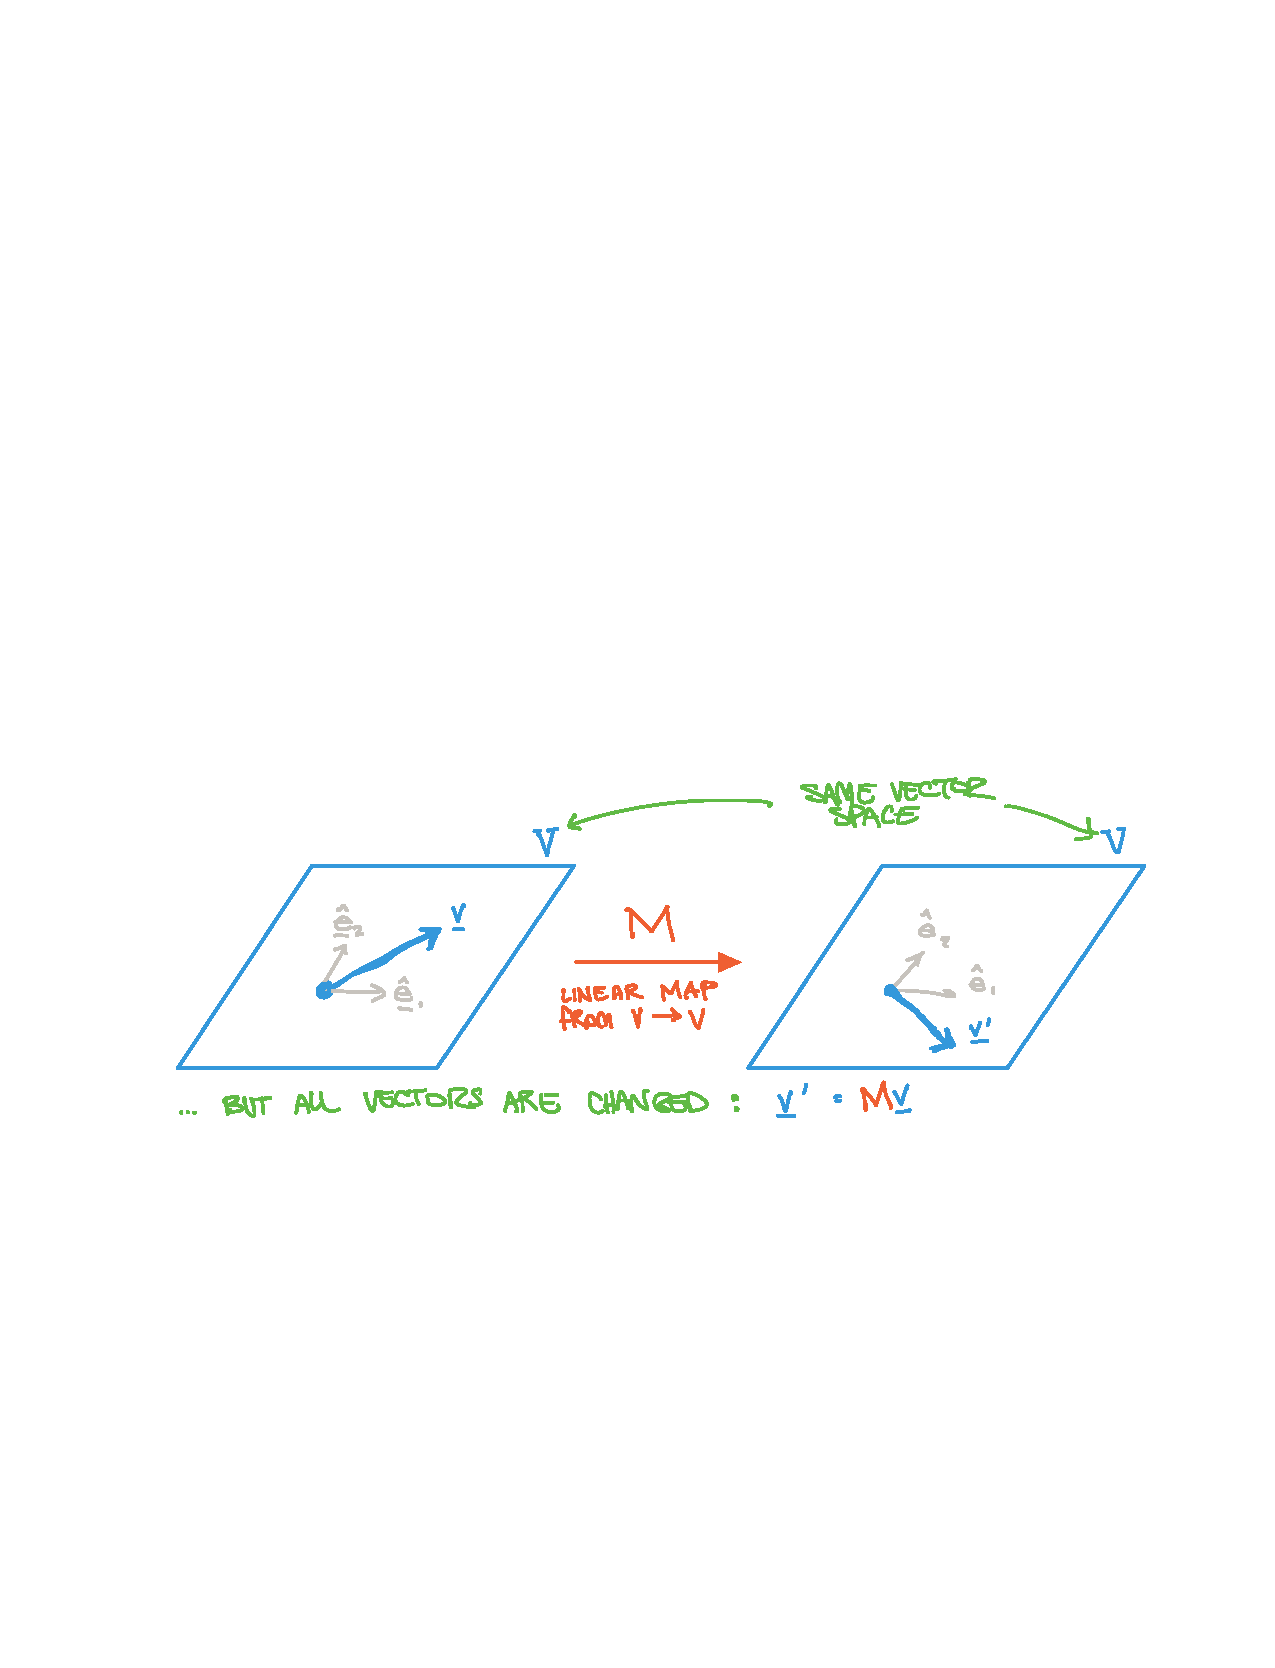
\includegraphics[width=\textwidth]{figures/lineartransformation.pdf}
\end{figure}


\begin{example}
Here are a few examples of each of the above terms:
\begin{itemize}
    \item A price checker at a store takes in barcodes and returns the cost of the item. This is a \emph{map} from barcodes to prices. This is not a map between vector spaces.\sidenotemark
    \item Conversion from kilograms to pounds is a \emph{map} takes a quantity in one unit and converts it to the same quantity in different units. This map is also \emph{linear}: if the input quantity is twice as heavy in kilograms, it will be twice as heavy in pounds. If you add two quantities in kilograms, the mass of the total object in pounds is the sum of the individual masses in pounds.
    \item A function that takes in a vector $\vec{v}\in\mathbbm{R}^2$ and returns $2\vec{v}$ is a transformation. Both the inputs and outputs are vectors in the same vector space. 
\end{itemize}
\end{example}\sidenotetext{At least I cannot figure out a reasonable vector space interpretation. I think I was already pushing it a bit far when we talked about cheeseburger-and-fries space in Example~\ref{ex:cheeseburger:space}.}

\paragraph{More jargon: one-to-one, onto, invertible}

We are going to make a big deal about \textbf{invertible transformations}\index{invertible}. An invertible transformation is one that can be reversed or undone. The transformation need not be linear---though our focus will be linear invertible functions---so for this paragraph let use write $\vec{f}(\vec{v})$ to mean an invertible, not-necessarily-linear transformation. I have even written the function as $\vec{f}$ rather than $f$ to remind us that the output is a vector. Mathematically, an invertible function is one where $\vec{f}^{-1}(\vec{v})$ is defined for any $\vec{v}$ and
\begin{align}
    \vec{f}\inv(\vec{f}(\vec{x})) = \vec{f}(\vec{f}\inv(\vec{x})) = \vec{x} \ .
\end{align}
The \emph{reason} why we care about invertible transformations is precisely the point in \bigidearef~\ref{idea:matrix:inverse:in:physics}: so much of physics is written in the form
\begin{align}
    (\text{operator})\, \ket{\text{state}} = \ket{\text{source}} \ ,
\end{align}
and our job is to invert the operator so that we can figure out what the state is as a function of the source. That is, we are usually given an equation
\begin{align}
    \vec{f}(\vec{x}) = \vec{w} \ ,
\end{align}
and we are given the form of the function $\vec{f}$ and the value of the source $\vec{w}$.\sidenote{Maxwell's equations are like this: on the left-hand side there's some fancy vector calculus differential operator acting on the field that you want to calculate, on the right-hand side there is some kind of charge or current distribution.} Our job is to determine $\vec{x} = \vec{f}\inv(\vec{v})$. 

Sometimes it is the case that $\vec{f}(\vec{x})$ is a pretty nasty function.\sidenote{By nasty I mean nonlinear. By nonlinear I mean \emph{not linear}, where the definition of linearity is \eqref{eq:linear:function}.} So instead of using $\vec{f}$, we can perform a Taylor expansion and consider the \emph{linear} part of $\vec{f}$. From our discussions so far, a linear transformation is represented as a matrix, $M$. Thus we end up writing:
\begin{align}
    \vec{f}(\vec{x}) \approx M\vec{x}  \ ,
\end{align}
and the problem inverting $\vec{f}$ reduces to the problem of inverting a linear transformation $M$. It is for this reason that we make a big deal about understanding when $M$ is invertible and, when it is, how to determine $M\inv$ in a systematic way.\sidenote{In Exercise~\ref{ex:matrix:inversino:the:hard:way} you already showed that finding the inverse of a matrix boils down to writing out and solving a system of equations. This method is intractable for very large matrices. Our goal is to reach infinite-dimensional matrices.}

\begin{example}
A function that takes your student identification number and returns your net\tacro{ID} is one-to-one. Every student identification number corresponds to a unique student with a unique net\tacro{ID}. However, not every net\tacro{ID} belongs to a student---faculty have net\tacro{ID}s but not student identification number, for example---so this function is not invertible. 
\end{example}

A few more bits of jargon. We won't use these, but consider these to be essential tools if you ever find yourself in a verbal sparring match with a mathematician:
\begin{enumerate}
    \item \textbf{Injective}\index{injective}/\textbf{one-to-one}\index{one-to-one}: 
    every output is unique; if you knew the output then you can deduce the input. However there may be some output-class objects that are not the outputs of the function for any input.
    \item \textbf{Surjective}\index{surjective}/\textbf{onto}\index{onto}: every output-class object is the result of some input, however there may be multiple inputs that produce the same output.
    \item \textbf{Bijective}\index{bijective}: this is a fancy name for \emph{invertible}. 
\end{enumerate}
% Every linear function is surjective. 

\begin{example}
Dual vectors are linear functions of vectors to numbers. Any non-zero dual vector $\row{w}$ is surjective. To see this, take any vector $\vec{v}$ and calculate $\row{w}\vec{v}$; call this number $a$. Any other number, say $b$, is the output of $\row{w}$ acting on $(b/a)\vec{v}$. Thus every output-class object (number) is realized as $\row{w}$ acting on some input. 
\end{example}

\begin{example}
In general, dual vectors are \emph{not} injective. For example, consider the dual vector $\row{w}=\begin{pmatrix}
    a & -a
\end{pmatrix}$. Then $\row{w}\vec{v} = 0$ for any vector $\vec{v}$ of the form
\begin{align}
    \vec{v} = 
    \begin{pmatrix}
        b \\ b
    \end{pmatrix}\ .
\end{align}
The zero vector is of this form so that $\row{w}\vec{0}=0$, as required by linearity. 
\end{example}


% Row vectors as 
% The fact that matrices take vectors and return vectors tells us that they enact transformations on the \emph{space} of vectors. Under the action of a matrix, every allowed vector is transformed into a different vector. 

\subsection{Basis of row vectors}

We write the basis row vectors as $\rbas{e}^i$ so that any row vector may be written $\row{w} = w_i \rbas{e}^i$. We have again chosen indices so that we may use summation convention. Everything that we have discussed about basis vectors in Section~\ref{sec:basis} carries over, except now the basis vectors are basis \emph{row} vectors. Because row vectors are themselves a vector space, this is not surprising. In fact, this is simply the \emph{duality} between $V$ and $V^*$. 

Now that we are armed with the idea of row vectors\sidenote{a.k.a\ dual vectors, covectors, bras} as linear transformations, we can go further and explain the nature of this duality. Fixing a basis of column vectors in $V$ automatically fixes the basis in $V^*$ in the following way:
% 
\begin{bigidea}[Basis of dual vectors]\label{idea:basis:of:dual:vectors}
Given a basis $\bas{e}_{1,\cdots,N}$ for a vector space $V$, the basis for the vector space $V^*$ is $\rbas{e}^{1,\cdots,N}$ and is defined as follows:
\begin{align}
    \rbas{e}^i\left[ \bas{e}_j \right] = \delta^i_j \ .
    \label{eq:basis:of:dual:vectors}
\end{align}
For example, $\rbas{e}^1\left[\bas{e}_2\right] = 0$ and $\rbas{e}^1\left[\bas{e}_1\right] = 1$.
\end{bigidea}
% 
This merits some reflection. Here is a sequence of thoughts:
\begin{enumerate}
    \item A basis dual vector is an linear map that takes in vectors and returns a number---this is our enlightened definition\sidenote{As opposed to a `sideways vector' or `the same thing as a vector,' which are slightly less enlightened (read: not useful, largely incorrect) definitions.} of a dual vector. 
    \item Because the map is linear, it is sufficient to define its action on a set of basis vectors. 
    \item Given a specific basis $\bas{e}_{1,\cdots,N}$ of the vector space $V$, there is a canonical\sidenote{Here canonical means ``correct choice.''} basis for $V^*$, \eqref{eq:basis:of:dual:vectors}. Each element of this canonical dual vector basis returns one when it is fed its `partner' vector basis element, and otherwise returns zero.
\end{enumerate}

Let us see this in action.

\paragraph{Basis dual vector eats a vector}
The vector itself is a linear combination of basis vectors: 
\begin{align}
    \vec{v} = v^i \bas{e}_i \ .
\end{align}
A [basis] dual/row vector is a linear function of vectors. This means that we can take any basis row vector $\rbas{e}^i$ and feed it the vector $\vec{v}$, we have
\begin{align}
    \rbas{e}^i\left[\vec{v}\right]
    =
    \rbas{e}^i\left[v^j\bas{e}_j\right]
    =
    v^j \rbas{e}^i\left[\bas{e}_j\right]
\ .
\end{align}
Note that the summation convention still holds, even though the basis vectors are in the jaws of the basis dual vector that is `eating' it. To be very clear, let us write this out explicitly for a two-dimensional vector space: 
\begin{align}
    \rbas{e}^i\left[\vec{v}\right]
    =
    \rbas{e}^i\left[ v^1\bas{e}_1 + v^1\bas{e}_1 \right]
    =
    v^1 \rbas{e}^i \left[\bas{e}_1\right] + v^2 \rbas{e}^i\left[\bas{e}_2\right]
\ .
\end{align}
Now we can invoke our defining rule for the basis dual vectors \eqref{eq:basis:of:dual:vectors}. We remember that Kronecker-$\delta$s collapse sums to a single element:
\begin{align}
    \rbas{e}^i\left[\vec{v}\right]
    =
    v^j \delta^i_j
    = v^j
\ ,
\end{align}
so that the $i^\textnormal{th}$ basis row vector $\rbas{e}^i$ acting on a vector simply returns the $i^\textnormal{th}$ component of the vector in the associated vector basis $\bas{e}_i$.
 

\paragraph{A dual vector as a linear combination of basis dual vectors}
A row vector is a linear combination of basis row vectors,
\begin{align}
    \row{w} = w_i\rbas{e}^i \ .
\end{align}
When we feed a row vector a column vector, each of the basis row vectors takes a bite:
\begin{align}
    \row{w}\vec{v} =
    w_i\rbas{e}^i\left[v^j\bas{e}_j\right]
    =
    w_i v^j \rbas{e}^i\left[\bas{e}_j\right]
    =
    w_i v^j \delta^i_j
    =
    w_i v^i \ ,
    \label{eq:linear:transformation:origin:of:summation}
\end{align}
which is \emph{precisely} the origin of the summation convention.

\begin{bigidea}[Origin of summation convention]
Given a basis for a vector space, there is a canonical basis of dual vectors given by \eqref{eq:basis:of:dual:vectors}. These basis dual vectors are linear functions of the vectors. The summation convention is a shorthand for what happens when a \emph{linear combination of basis vectors} $\vec{v}$ are fed to a \emph{linear combination of basis dual vectors} $\row{w}$. The notation is extended to tensors, which are linear maps between multiple copies of $V$ and $V^*$. These are called multi-linear maps because they are linear in each index.
\end{bigidea}

\begin{exercise}\label{ex:vector:act:on:row}
In this section we have defined basis dual vectors as the `eaters of vectors.' Of course, the nature of this duality is that we may \emph{equivalently} treat vectors as the `eaters of row vectors.'\sidenotemark Rewrite all of the results in this section by treating row vectors as the food and column vectors as the linear function. Confirm that it is \emph{obvious} that the analog of \eqref{eq:basis:of:dual:vectors} is
\begin{align}
    \bas{e}_i\left[\rbas{e}^j\right] = \delta^j_i \ .
    \label{eq:basis:of:dual:vectors:reverse}
\end{align}

\end{exercise}\sidenotetext{The fancy way of saying this is that $(V^*)^* = V$. The space of linear functions on row vectors is exactly the space of vectors.}



% change of basis on row vectors: rotates oppositely!


\subsection{Duality and the Bra-Ket Notation}

This is one place where the bra-ket notation of quantum mechanics starts to shine. As a reminder, vectors are written as kets,
\begin{align}
    \vec{v} \defeq \ket{v} \ .
\end{align}
There is \emph{no content} in this equation! It simply defines an equivalent notation for vectors. We write the basis kets as\sidenote{Sometimes it is expedient to simply write $\ket{e_i} = \ket{i}$, but then you lose the reminder that it has a lower index.}
\begin{align}
    \bas{e}_i \defeq \ket{e_i} \ .
\end{align}
This means that a vector is
\begin{align}
    \ket{v} &= v^i\ket{e_i} \ .
\end{align}
% 
Similarly, row vectors are bras with associated basis bras:
\begin{align}
    \row{w} &\defeq \bra{w} & \rbas{e}^i &\defeq \bra{e^i}
    & \bra{w} &= w_i \bra{e^i} \ .
\end{align}


Now the duality expressed in Exercise~\ref{ex:vector:act:on:row} is clear because we just think of the vertical edge of the bra or ket being its \emph{interface} with the other type. The duality relations \eqref{eq:basis:of:dual:vectors} and \eqref{eq:basis:of:dual:vectors:reverse} reduce to a single relation:
\begin{align}
    \la e^i \mid e_j \ra = \delta^i_j \ .
    \label{eq:defining:bra:ket:relatin}
\end{align}
Then the action of a bra on a ket is manifestly symmetric with the action of a ket on a bra. They are the same thing:
\begin{align}
    \la w \mid v \ra &= w_iv^j \la e^i \mid e_j \ra  = w_i v^j \delta^i_j = w_iv^j \ .
    \label{eq:basis:of:dual:vectors:bra:ket:form}
\end{align}

\subsection{Basis of matrices}

Matrices have one upper index and one lower index. If we think about matrices as squares of numbers,\sidenote{... and one of the goals of this course is to go \emph{beyond} thinking of matrices this way.} then we can imagine what a basis of matrices looks like. For a $2\times 2$ matrix $M$,
\begin{wide}
 \begin{align}
        M=
     \begin{pmatrix}
         M\aij{1}{1} & M\aij{1}{2}\\
         M\aij{2}{1} & M\aij{2}{2}
     \end{pmatrix}
     &= 
     M\aij{1}{1} 
     \begin{pmatrix}
     1 & 0 \\
     0 & 0    
     \end{pmatrix}
     + M\aij{1}{2}
     \begin{pmatrix}
     0 & 1 \\
     0 & 0    
     \end{pmatrix}
     + M\aij{2}{1} 
     \begin{pmatrix}
     0 & 0 \\
     1 & 0    
     \end{pmatrix}
     + M\aij{2}{2}
     \begin{pmatrix}
     0 & 0 \\
     0 & 1    
     \end{pmatrix}
\end{align} \ .
\label{eq:M:2:2:basis:of:matrices:0}
\end{wide}
We can write this succinctly in bra-ket notation as follows:
\begin{align}
    \begin{pmatrix}
         M\aij{1}{1} & M\aij{1}{2}\\
         M\aij{2}{1} & M\aij{2}{2}
     \end{pmatrix}
     &= 
     M\aij{i}{j} \ket{e_j}\!\bra{e^i} \ .
     \label{eq:M:2:2:basis:of:matrices:1}
\end{align}
Does this make sense? Evidently it implies that $\ket{j}\!\bra{i}$ encodes the $2\times 2$ matrix that has a one on the $i$--$j$ component and zeroes everywhere else.
% 
Does this, in turn, make sense? $\ket{e_j}\!\bra{e^i}$ is a machine that, when acting on a vector, does two things:
\begin{enumerate}
    \item It takes in a vector and pulls out the $i^\text{th}$ component,
    \item then it places that into the $j^\text{th}$ component of the output vector.
\end{enumerate}
\begin{exercise}
Confirm that $\ket{e_j}\!\bra{e^i}$ behaves as described above.
\end{exercise}
This is precisely the action of a matrix that is zero except for the $i$--$j$ component, which is one. For example:
\begin{align}
    \begin{pmatrix}
    0 & 0\\
    1 & 0  
    \end{pmatrix}
    \begin{pmatrix}
        v^1 \\
        v^2
    \end{pmatrix}
    &= 
    \begin{pmatrix}
        0 \\
        v^1
    \end{pmatrix} \ 
    &
    \ket{e_2}\!\la{e^1} \mid v\ra 
    &= 
    v^1 \ket{2} \ .
\end{align}
We have used the defining relation of the bra (dual vector) bases, \eqref{eq:basis:of:dual:vectors:bra:ket:form}. So we see that indeed the bases in \eqref{eq:M:2:2:basis:of:matrices:0} and \eqref{eq:M:2:2:basis:of:matrices:1} are identical. 

The ket-bra $\ket{j}\!\bra{i}$ is an example of a tensor product\index{tensor product}, a phrase we first use in \eqref{eq:M:tensor:product}. Poetically, this tensor product is gluing together two machines: a vector and a dual vector. Each machine is simultaneously an object (vectors are acted on by dual vectors) and a linear functions that acts on objects to produce numbers (vectors also act on dual vectors). The idea in Section~\ref{sec:linear:maps} that a matrix is many different kinds of linear maps\sidenote{Recall that a matrix can be understood as any of the following: $V\otimes V^*\to \#$, $V\to V$, or $V^* \to V^*$.} is simply a choice of the different combinations of whether the machines are treated as objects or the linear functions acting on objects. 
 
Sometimes, if we are feeling fancy, we may write this using that fancy X-Men symbol:\sidenote{As this is being written, the animated series \emph{X-Men '97} is airing and the ``Fall of X'' story arc of the comic series is drawing to a close.}
\begin{align}
    \ket{e_j}\!\bra{e^i} = \ket{e_j} \otimes \bra{e^i} = \bas{e}_i \otimes \rbas{e}^j \ .
\end{align}
The \sout{X-Men symbol} tensor product is there to remind us that these bras (dual vectors) and kets (vectors) are not acting on each other.  Otherwise the expression on the right may be confused with\sidenote{This is the sense in which $V=(V^*)^*$; vectors are themselves dual to dual vectors.} 
\begin{align}
\bas{e}_i \rbas{e}^j \stackrel{?}{=}
    \bas{e}_i[\rbas{e}^j] = \delta^j_i \ ,
\end{align}
which it is \emph{not}. This is another benefit of the bra-ket notation.


Let us recover our rule for matrix multiplication using this notation. We start by writing a matrix acting on a vector:
\begin{align}
    M\vec{v} &= 
    M\aij{i}{j}\ket{e_i}\!\bra{e^j}\; 
    v^k\ket{e_k}
    =
    M\aij{i}{j} 
    v^k\; 
    \ket{e_i}\!\la{e^j} \mid {e_k} \ra
    % =
    % M\aij{i}{j} 
    % v^k\; \delta^{k}_j \; \ket{e_i}
    =
    M\aij{i}{j} 
    v^j\; \ket{e_i} \ .
\end{align}
We have used our one defining relation, $\la{e^j} \mid {e_k} \ra = \delta^j_k$, and simply pulled all the \emph{numbers}/\emph{coefficients}---$M\aij{i}{j} v^k$---from all of the tensorial stuff---the bras and kets. 

\begin{bigidea}[Columns to indices to maps]\index{idea:columns:to:indices:to:maps}
Appreciate what has happened here. In Chapter~\ref{ch:basics} we introduced the `matrix multiplication' picture where we treated vectors as columns of numbers and matrices as square arrays of numbers. Then in Chapter~\ref{ch:vectors:row:matrices:in:indices} we replaced that picture with a different one based on indices. In Section~\ref{sec:treachery:of:indices:vi:is:not:a:vector} we reflected on the ambiguity of expressions like $\vec{v}\simeq v^i$: does $v^i$ refer to a vector, or a \emph{component} of a vector? Now we have gone one layer deeper and explained that there was a in the index-only picture that had been implicit: the notion of a basis. Furthermore, this basis is rigorously understood in the language of linear maps. 

Using the defining feature of row versus column basis vectors \eqref{eq:M:2:2:basis:of:matrices:0}, we derive the index contraction rule that was an assumption in the intermediate index-only picture. Granted, we have \emph{invented} this `deeper structure,' but this invention is meaningful. It defines the \emph{duality} between $V$ and $V^*$ and gives us a functional understanding of index contraction.
\end{bigidea}

As another illustrative example, the multiplication of two matrices. Now we have
\begin{align}
    M\aij{i}{j} \ket{e_i}\! \bra{e^j} \quad N\aij{k}{\ell}  \ket{e_k}\!\bra{e^\ell}
    &=
    M\aij{i}{j} N\aij{k}{\ell} \quad \ket{e_i} \la{e^j} \mid {e_k}\ra \bra{e^\ell}
    \label{eq:basis:matrix:mult:MN}
    \\&=
    M\aij{i}{j} N\aij{k}{\ell}\, \delta^k_j \quad \ket{e_i}\!\bra{e^\ell} 
    \\&=
    M\aij{i}{j} N\aij{j}{\ell} \; \ket{e_i}\!\bra{e^\ell} \ ,
\end{align}
from which we read that the $i$--$\ell$ component of the matrix $MN$ is $ M\aij{i}{j} N\aij{j}{\ell}$ \ .

This basis and the bra-ket notation also gives a convenient way to express the \textbf{trace}\index{trace} of a matrix---or more generally, the contraction of an upper and lower index of the same tensor. The trace operation is
\begin{align}
    \Tr(\cdots) = 
    \bra{e^i} \cdots \ket{e_i} \ .
\end{align}
For a matrix:
\begin{align}
    \Tr M &= \bra{e^i}\; \left(M\aij{k}{\ell}\ket{e_k}\!\bra{e^\ell}\right) \;\ket{e_i}
    = M\aij{k}{\ell}  
    \la {e^i} \mid {e_k}\ra \, \la {e^\ell} \mid {e_i} \ra 
    \\
    &= 
    M\aij{k}{\ell}  \delta^i_k \delta^\ell_i 
    =  M\aij{i}{i} \ .
\end{align}
Indeed we recover our usual index-based definition, which in turns was a sophisticated way of saying ``sum the diagonal components of a square array of numbers.'' Observe that the bra-ket notation really shined her: this would have been a minor pain to describe using the $\bas{e_i}$ and $\bas{e^j}$ expressions.


\begin{example}[Choosing a contraction]\label{eg:contraction:choices}
In \eqref{eq:basis:matrix:mult:MN} we multiplied two matrices,
\begin{align}
     M\aij{i}{j} \ket{e_i}\! \bra{e^j} \quad N\aij{k}{\ell}  \ket{e_k}\!\bra{e^\ell} \ .
\end{align}
How do we \emph{know} which of the basis bras and kets are hitting each other? In that case, we \emph{assumed} that the $\bra{e^j}$ acts on the $\ket{e_i}$. This gave the conventional definition that the lower index of $M$ contracts with the upper index of $N$. 

Alternatively, we could have said that the $\bra{e^\ell}$ contracts with the $\ket{e_i}$. That gives:
\begin{align}
    M\aij{i}{j} N\aij{k}{\ell} 
    \quad \ket{e_k}\! \bra{e^j}   \la {e^\ell} \mid {e_i} \ra
    &=
    M\aij{i}{j} N\aij{k}{\ell}\, \delta^\ell_i \quad \ket{e_k}\! \bra{e^j}
    \\&=
    M\aij{i}{j} N\aij{k}{i} \; \ket{e_k}\! \bra{e^j}
    \\&=
    N\aij{k}{i}M\aij{i}{j} \; \ket{e_k}\! \bra{e^j}\ .
\end{align}
Follow this carefully: all that differs from \eqref{eq:basis:matrix:mult:MN} is that we \emph{demanded by fiat}\footnote{We literally just wrote it in words. There is no mathematical notation that showed which ket and which bra are contracting, it is something that is \emph{understood before} we wrote the equation. Some people have made up notation---look up bird tracks---but for most cases this is complete overkill.} that a different bra/ket pair act on each other. The result is that instead of what we normally call $MN = M\aij{i}{j}N\aij{j}{\ell}$, we ended up with what we normally call $NM= N\aij{k}{i}M\aij{i}{j}$. In hindsight, this is not so surprising: given two matrices, there are two ways to combine them to get another matrix. In the old matrix multiplication language of Section~\ref{sec:matrix:multiplication}, we would call these $MN$ and $NM$ and comment on how matrix multiplication does not commute. In our linear map picture of tensors, we see that this really boils down to \emph{choosing} which of the two possible ways that the bras and kets can act on each other. 

In a given physical situation, how are you suppose to know which basis bras and kets are supposed to contract? It is almost always the case that this is either obvious\footnote{Examples for why the bra/ket action may be obvious: perhaps someone is using the old `matrix multiplication' language so you know that bras act on adjacent kets, or perhaps because you know the physical meaning of what the matrix does and there is a particular transformation that you are performing.} or otherwise it is communicated explicitly in words. 
\end{example}

\begin{exercise}\label{eq:matrix:product:trace}
In the multiplication of the two matrices in \eqref{eq:basis:matrix:mult:MN}, one could have also demanded that \emph{all} of the bras and kets contract. There are two ways of doing this. In one case, you get the product of the traces of each matrix:
\begin{align}
    (\Tr{M})(\Tr{N}) = M\aij{i}{i} N\aij{j}{j} \ .
\end{align}
Show that in the other case you get the trace of the product, $\Tr{MN}$. Show that $\Tr{MN} = \Tr{NM}$.
\end{exercise}

% again a place where the bra ket notation shines, much harder to write this using e's.



 \subsection{Basis of tensors}

 We may generalize to tensors by writing a generic tensor as:
 \begin{align}
    T =
     T\aij{i_1\cdots i_N}{j_1\cdots j_M}
     \ket{e_{i_1}}\cdots \ket{e_{i_N}}
     \bra{e^{j_1}}\cdots \bra{e^{j_M}} \ .
     \label{eq:tensor:T:with:basis}
 \end{align}
\begin{exercise}
Show how the index rules for tensors contraction onto other objects works using the bra-ket basis notation. Try making up some tensors, say $T^{ij} \ket{e_i}\ket{e_j}$ to see how it can contract onto other objects and use the defining relation \eqref{eq:basis:of:dual:vectors:bra:ket:form} to derive the usual index contractions. 
\end{exercise}

\begin{bigidea}[Tensors as linear functions]\label{idea:tensor:as:function}
Tensors are linear maps from some number of copies of $V$ and $V^*$ to numbers: a $(p,q)$ tensor is a map from $V^q \times (V^*)^p \to \#$. If we write such a tensor as $T\aij{i_1\cdots i_p}{j_1\cdots j_q}$, then these indices may contract with $p$ lower indices and $q$ upper indices to give a number. This is equivalently understood as a \emph{multi-linear} machine that takes in $q$ vectors and $p$ dual vectors to return a number. Here mutli-linear means that the machine is linear in each argument. 
\end{bigidea}

\begin{example}
Consider the $(2,1)$ tensor $T$ with components $T\aij{ij}{k}$. This is a map from $V\times V \times V^* \to \#$ because we may feed it a vector, $v^i$, and two row vectors, $w_j$ and $u_k$ to contract into a number:
\begin{align}
    T(\row{w},\row{u}, \vec{v})
    &=
    T\aij{ij}{k}v^k w_i u_j \ .
\end{align}
\end{example}

\begin{bigidea}[Tensors as linear maps]\label{idea:tensor:as:map}
Tensors are also linear maps between copies of vector spaces and dual vector spaces into other copies of vector spaces and dual vector spaces depending how its indices contract with other objects. A $(p,q)$ tensor $T$ may contract with an $(r,s)$ tensor $S$ such that:
\begin{itemize}
    \item Anywhere 
    \item from 0 to $\min(p,s)$ the upper indices of $T$ are contracted with the pairs of the lower indices of $S$.
    \item Anywhere from 0 to $\min(q,r)$ of the lower indices of $T$ are contracted with the upper indices of $S$.
\end{itemize}
Depending on these choices, the resulting object is a $(m,n)$ tensor where 
\begin{itemize}
    \item $m$ is from $[(p+q) - \min(p,s) - \min(q,r)]$, in the case of maximal contractions, to $(p+q)$, in the case of no contractions.
    \item $n$ is from $[(s+r) - \min(p,s) - \min(q,r)]$, in the case of maximal contractions, to $(s+r)$, in the case of no contractions.
\end{itemize}
\end{bigidea}

\begin{example}[Maps between product spaces]\label{eg:maps:between:product:spaces}
Example~\ref{eg:contraction:choices} and Exercise~\ref{eq:matrix:product:trace} demonstrate this for the case of two (1,1) tensors. 

Consider the case of a $(2,1)$ tensor $T\aij{ij}{k}$. Here are some possible contractions with different kinds of objects (we suppress the basis tensors and only write the components):
\begin{itemize}
    \item $T\aij{ij}{k}v^k$ is a (2,0) tensor $(T\vec{v})^{ij}$.
    \item $T\aij{ij}{k}w_i$ is a (1,1) tensor $(T\row{w})\aij{j}{k}$.
    \item $T\aij{ij}{k}M\aij{k}{\ell}$ is a (2,1) tensor $(TM)\aij{ij}{\ell}$
    \item $T\aij{ij}{k}M\aij{k}{j}$ is a (1,0) tensor $(TM)^i$.
    \item $T\aij{ij}{k}M\aij{\ell}{j}$ is a (2,1) tensor $(TM)\aij{ik}{\ell}$.
    \item $T\aij{ij}{k}T\aij{k\ell}{m}$ is a (3,1) tensor $(T^2)\aij{ij\ell}{m}$.
    \item $T\aij{ij}{k}T\aij{k\ell}{j}$ is a (2,0) tensor $(T^2)^{i\ell}$.
\end{itemize}
As practice, you are welcome to confirm all of this by including the bases `ket-bra' tensors. 
\end{example}

\begin{example}[Why ket-bras?]\label{eg:why:ketbra}
When writing a generic tensor in terms of its basis, say $T$ in \eqref{eq:tensor:T:with:basis}, we typically write these with kets first then bras.\sidenotemark This is a convention that makes it clear that none of the kets are acting on any of the bras.

What if you have a tensor where the order of the indices do not match the kets-first-then-bras convention? For example, a tensor:
\begin{align}
    Y = Y^{ij\phantom{k}\ell}_{\phantom{ij}k}
    \ket{e_i}\otimes\ket{e_j}\otimes\bra{e^k}\otimes\ket{e_\ell} \ ,
\end{align}
where we have used the \sout{X-men} tensor symbol $\otimes$ to make it clear that none of the bras or kets are acting on each other. This avoids any ambiguity, but it is cumbersome to write. (At least not without humming the theme song of the X-men animated series from the 1990s.)

In these cases, it is useful to simply \emph{define} a tensor where the order of indices is more convenient, but that otherwise contains the same information:
\begin{align}
    W = W\aij{ij\ell}{k} 
    \ket{e_i}\ket{e_j} \ket{e_k} \bra{e_\ell}
    \defeq 
    Y^{ij\phantom{k}\ell}_{\phantom{ij}k}
    \ket{e_i} \otimes \ket{e_j} \otimes \bra{e^k} \otimes \ket{e_\ell}
    \ .
\end{align}
This amounts to the component-wise identification
\begin{align}
    W\aij{ij\ell}{k} \equiv Y^{ij\phantom{k}\ell}_{\phantom{ij}k} \ .
\end{align}

\end{example}\sidenotetext{Notationally, kets and bras act on each other when the vertical lines match up, not when their angled parts point at each other.}

Observe that it can sometimes be ambiguous to know which bras and which kets are contracting with one another, so one may have to specify this explicitly. That is: if $T^{ij} \ket{e_i}\ket{e_j}$ is acting on $w_k\bra{e^k}$, which of $\ket{e_i}$ or $\ket{e_j}$ hits the $\bra{e^k}$? 

Practically when one has a tensor with several of the same type of basis bra or ket, one ends up symmetrizing or antisymmetrizing any contraction. This amounts to separating a tensor like $T^{ij} = T^{ij}_\textnormal{s} + T^{ij}_\textnormal{a}$ into a symmetric piece with $T_\textnormal{s}^{ij} = T_\textnormal{s}^{ji}$ and an antisymmetric piece with $T_\textnormal{a}^{ij}=-T_\textnormal{a}^{ji}$. Having done this, it does not matter \emph{which} of the `identical' indices you contract with because they are all treated on the same footing---at least up to a minus sign for the antisymmetric case. See Section~\ref{sec:permutation:symmerty} for the case of two lower indices. This sort of symmetrizing/antisymmetrizing game shows up in the representation theory of symmetries.
% Example: H2 dissociation

\begin{exercise}
Let $B_{ij}\bra{e^i}\bra{e^j}$ be a $(0,2)$ tensor. Separate it into a symmetric and an antisymmetric piece, $B = S+A$ where $S_{ij} = S_{ji}$ and $A_{ij} = - A_{ji}$. Assuming you know each component $B_{ij}$, write out each component $S_{ij}$ and $A_{ij}$.

Let $\vec{v} = v^i\ket{e_i}$ be a vector. Show that $B\ket{v}\ket{v} = S\ket{v}\ket{v}$. That is, show that
\begin{align}
    A\ket{v}\ket{v} = 0 \ .
\end{align}

Let $C^{ij}\ket{e_i}\ket{e_j}$ be an \emph{antisymmetric} $(2,0)$ tensor so that $C^{ij} = C^{ji}$. Show that $BC = AC$, or otherwise that
\begin{align}
    SC = 0 \ .
\end{align}

\textsc{Comment}: in each of these questions, there should be no ambiguity about which bras and which kets are contracted. If you worry that you have to make an arbitrary choice, check that the (anti-)symmetrization means that it does not actually matter up to a minus sign, provided that all objects that have multiple upper and/or multiple lower indices are symmetrized or anti-symmetrized.
\end{exercise}

 

\section{Transformation under symmetries}
\label{sec:transformation:under:symmetries}

Let us return to dancing around the really-big-idea of symmetries, even though we continue to be coy about actually defining these. We first introduced rotations in Section~
\ref{sec:Euclidean:three:space:rotations}, where we pontificated about the relation of rotations to the dot product because rotations leave vector lengths and angles between vectors unchanged. In Section~\ref{sec:isometry:first:pass:indices} we defined Rule~\ref{idea:transformation:of:upper:and:lower:indices} that told us how objects with indices transform. For example, in two-dimensional Euclidean space rotations that move the positive $x$-axis\sidenote{Here I should really say the $\bas{e}_1$ axis rather than the $x$-axis. This is because $x$ and $y$ are typically the coordinates what is called a `base space' or a base \emph{manifold}. In this section we refer to $x,y,$ and $z$ to appeal to our familiarity with three-space.} counter-clockwise (towards the positive $y$ axis) by and angle $\theta$ are $2\times 2$ matrices of the form
\begin{align}
    R(\theta)=
    \begin{pmatrix}
        \cos\theta & -\sin\theta \\
        \sin\theta & \pp \cos\theta
    \end{pmatrix} \ .
\end{align}
The following exercises introduce some of the machinery for rotations.
\begin{exercise}
If you have not done so yet, please confirm that $R(\theta)^\trans = R(\theta)\inv = R(-\theta)$.
\end{exercise}
\begin{example}
In three dimensions there are more kinds of rotations. One way to characterize this is to consider rotations about each coordinate axis. 
\begin{align}
    R_x(\theta) &= 
    \begin{pmatrix}
        1 & & \\
        &  \cos\theta & -\sin\theta \\
        & \sin\theta &  \pp\cos\theta 
    \end{pmatrix}
    \\
    R_y(\theta) &= 
    \begin{pmatrix}
        \pp \cos\theta & &\sin\theta \\
        & 1 & \\
        -\sin\theta& & \cos\theta
    \end{pmatrix}
    \\
    R_z(\theta) &= 
    \begin{pmatrix}
       \cos\theta & - \sin\theta & \\
        \sin\theta &\pp \cos\theta & \\
        & & 1
    \end{pmatrix}\ ,
    \label{eq:3D:rotation:matrices}
\end{align}
where all unlisted components are zero. Notice that these are all reshufflings of the rotations of the plane with the rotation axis held fixed---that should make sense. Also notice that the $R_y(\theta)$ rotation has the $-\sin\theta$ term in the lower-left while the other two rotations have it on the upper-right. This is to consistently apply the right-hand rule convention: a rotation about the $i^\textnormal{th}$ axis corresponds to gripping the axis with your right hand so that your thumb is pointing along the positive direction and identifying the direction that your fingers curl as the rotation direction. For each of these matrices, $R_i(\theta)^\trans = R_i(\theta)\inv = R_i(-\theta)$. 
\end{example}
\begin{exercise}
Taylor expand each of the three matrices in \eqref{eq:3D:rotation:matrices} and write them each in the form
\begin{align}
    R_i(\theta) = \one + i T_i \theta + \mathcal O(\theta^2) \ .
\end{align}
Here $i$ is the imaginary number, $i^2=1$, and the matrix $T_i$ is also pure imaginary.\footnote{This factor of $i$ is a convention in physics.} 

\textsc{Comment:}
The $T_i$ matrices are called \textbf{generators} each type of rotation. Physically, they represent the effect of an infinitesimal rotation about the respective axes. Infinitesimal rotations about other axes are given by \emph{linear combinations} of the $T_i$. In this way, the $T_i$ are a \emph{basis} for rotations.

Show that $T_xT_y - T_y T_x \propto T_z$ and determine the constant of proportionality. This relation is called an \emph{algebra} and denotes the mathematical structure of rotational symmetry.\footnote{This symmetry is called \SO{3}, the special orthogonal group of rank 3. Special means unit determinant, orthogonal means $R^\trans R = \one$.}
\end{exercise}

\begin{exercise}
The \emph{generator} of \SO{2}, rotations of the Euclidean plane, is
\begin{align}
    T = \begin{pmatrix}
        0 & i \\
        -i & i
    \end{pmatrix} \ .
\end{align}
Show that $R(\theta) = \exp(iT\theta)$ where the matrix exponential is defined as its power series:
\begin{align}
    e^{M} = 1 + M + \frac{1}{2}M^2 + \cdots \ .
\end{align}
Use the power series expansion of the trigonometric functions. 
\end{exercise}

Assuming that we have a definition for which transformations are rotations,\sidenote{More generally, which transformations are \emph{isometries}. We finally present such a definition in Chapter~\ref{ch:metric:spaces}.} then we can examine how the basis vectors and row vector transform.

% Motivating the indices
% What is a symmetry



\subsection{Transformation of Vectors}

To be somewhat philosophical: under an isometry like a rotation, there are two pictures to think about what happens to a vector:
\begin{itemize}
    \item \textbf{Active transformation}\index{active transformation}: your basis vectors stay put, but the vector is changing into a different vector, $\ket{v} \to \ket{v'}$. The components of $\ket{v'}$ are clearly different from the components of $\ket{v}$ because it the two are simply not the same vector.
    \item \textbf{Passive transformation}\index{passive transformation}: the vector \emph{does not change}, but the basis vectors change, $\ket{e_i} \to \ket{e'_i}$. This means that the components of $\ket{v}$ must \emph{also} change so that $v^i\ket{e_i} = v'^{i}\ket{e_i}$.
\end{itemize}
In an active transformation, the vector space and every vector in it change. In a passive transformation, the observer changes.\sidenote{There is something oddly Zen and philosophical about this.} For an isometry---a symmetry of the system---either perspective is valid. 
% 

Let $R(\theta)$ be the rotation about some axis by some angle $\theta$ that enacts a symmetry transformation. In the passive picture, vectors remain unchanged, but the basis vectors and the corresponding components do change:
\begin{align}
    \ket{v} = v^i \ket{e_i} =
    % v^i R\inv R \ket{e'_i}
    v^\ell R\aij{i}{\ell} (R\inv)\aij{\ell}{k}  \ket{e_k} \
    \defeq (v')^\ell \ket{e'_\ell}
    \ .
\end{align}
In the second equality we have simply inserted $\one = R R\inv$. On the right-hand side we \emph{define} the rotated components $v'$ and rotated basis vectors $\ket{e'}$ by absorbing the $R$ and $R\inv$ rotations:
\begin{align}
    (v')^i &\defeq R\aij{i}{\ell} v^\ell
    &
    \ket{e'_i} &\defeq  (R\inv)\aij{j}{i}\ket{e_j} \ .
    \label{eq:passive:transformation:of:vector:and:basis}
\end{align}
All we have done is collect into $v'^i$ all objects that contract with $v^ell$ and leave an object of a single upper index: that means that we absorb the $R\aij{i}{\ell}$. Similarly, we collect into $\ket{e'_i}$ all objects that contract with $\ket{e_j}$ and leave an object of a single lower index: that means we absorb the $(R\inv)\aij{j}{i}$. From this we have \emph{derived} the ``indexology rule'' \eqref{eq:components:of:vector:and:row:under:rotatino} which led us to the general tensor transformation in \bigidearef{}~\ref{idea:transformation:of:upper:and:lower:indices}.

Let me say that one more time: in \eqref{eq:passive:transformation:of:vector:and:basis} we are not \emph{applying} the rule that upper indices transform with $R$ and lower indices transform with $R\inv$. In fact, we are \emph{deriving it} from the condition that a passive [symmetry] transformation leaves the vector $\ket{v}$ unchanged while simply changing the basis and components of $\ket{v}$ while preserving $\ket{v}$.



To be clear, this choice of active versus passive pictures is only true for symmetries (isometries) where in some sense the system is not meaningfully changing. A general transformation that is \emph{not} an isometry should be thought of as an active transformation that change vectors.
\begin{example}
If we were to rotate the entire solar system, then it does not matter too much whether we think about this as some cosmic entity actually changing the configuration of every celestial object \emph{or} if we simply choose a rotated set of coordinates for the solar system. However, if we were to \emph{stretch} the solar system along one axis of the plane of the planets' rotation, then all of a sudden the planets would not be in stable orbits.\sidenotemark
\end{example}\sidenotetext{In this hypothetical: the coordinates do not change and Newton's laws do not change. Thus stretching the positions of each of the plants pulls them further away from the center of the sun without changing their angular momentum.}


\subsection{Transformation of Row Vectors}

The same argument holds for row vectors. For an isometry, one may take the passive transformation perspective in which row vectors do not transform, but we transform both the basis row vectors $\bra{e^i}$ and components of the row vector $w_i$ in such a way that $\bra{e^i}w_i \to \bra{{e'}^i}w'_i = \bra{w}$: 
\begin{align}
    w'_i &\defeq \tilde R\aij{\ell}{i} w_\ell
    &
    \bra{e'^i} &\defeq  (\tilde{R}\inv)\aij{i}{j}\bra{e^j} \ .
    \label{eq:passive:transformation:of:row:vector:and:basis}
\end{align}
In principle, this rotation $\tilde R$ is a different rotation from $R$. One may think think that $\tilde R$ has \emph{nothing to do} with the transformation of vectors, $v^i\ket{e_i} \to R\aij{i}{k}v^k(R\inv)\aij{\ell}{i}\ket{e_\ell}$. However, if $R$ and $\tilde R$ enact a symmetry of the system, then the transformations must preserve the defining relation of the dual vector basis \eqref{eq:basis:of:dual:vectors}, or the bra-ket form of that rule \eqref{eq:basis:of:dual:vectors:bra:ket:form}. This means we want to impose
\begin{align}
    \la e'^i \mid e'_j \ra \equiv \delta^i_j \ .
    \label{eq:basis:transform:under:rotation}
\end{align}
Inserting our expressions of the passively rotated basis elements relative to the original basis elements,\sidenote{We do this because we assume that the original basis elements satisfy $\la e^i \mid e_j \ra \equiv \delta^i_j$.}
\begin{align}
    \la e'^i \mid e'_j \ra &= 
    \la e^k \mid (\tilde{R}\inv)\aij{i}{k} (R\inv)\aij{\ell}{j} \mid e_\ell \ra
    =
    (\tilde{R}\inv)\aij{i}{k} (R\inv)\aij{\ell}{j} \la e^k \mid e_\ell \ra
    \\
    &=
    (\tilde{R}\inv)\aij{i}{k} (R\inv)\aij{\ell}{j} \delta^k_\ell
    =
    (\tilde{R}\inv)\aij{i}{k} (R\inv)\aij{k}{j} \ .
\end{align}
In order for this to equal $\delta^i_j$ we must have
\begin{align}
    (\tilde R)\inv R\inv = \one \ ,
\end{align}
or equivalently
\begin{align}
    \tilde R = R\inv \ ,
\end{align}
which is precisely what we motivate below \eqref{eq:R:Rtilde:transformation:from:indices:rotation}. 


\subsection{Transformation of Tensors}

Having established how $\ket{e_i}$ and $\bra{e^j}$ transform, the transformation of a general tensor---one composed of the tensor product of some number of bras and some number of kets---follows simply from the transformation of each bra and ket individually.

\begin{wide}
In this way, we may augment Rule~\ref{idea:transformation:of:upper:and:lower:indices} and \eqref{eq:transformation:of:upper:and:lower:indices} with the statement that from the passive transformation perspective, the basis tensors transform as
\begin{align}
    % T\aij{i_1\cdots i_N}{j_1\cdots j_M}
    % \to 
    % R\aij{i_1}{k_1}\cdots R\aij{i_N}{k_N}
    % (R\inv)\aij{\ell_1}{j_1}\cdots (R\inv)\aij{\ell_N}{j_N}
    % T\aij{k_1\cdots k_N}{\ell_1\cdots \ell_M} \ .
    % \label{eq:transformation:of:upper:and:lower:indices}
    \ket{e_{i_1}} \cdots \ket{e_{i_N}}
    \bra{e^{j_1}} \cdots \bra{e^{j_M}}
    \to 
    (R\inv)\aij{k_1}{i_1}\cdots (R\inv)\aij{k_N}{i_N}
    R\aij{j_1}{\ell_1}\cdots R\aij{j_N}{\ell_M}
    \ket{e_{k_1}} \cdots \ket{k_{i_N}}
    \bra{e^{\ell_1}} \cdots \bra{e^{\ell_M}} \ .
\end{align}
For completeness, here is how the components transform:
\begin{align}
    T\aij{i_1\cdots i_N}{j_1\cdots j_M}
    \to 
    R\aij{i_1}{k_1}\cdots R\aij{i_N}{k_N}
    (R\inv)\aij{\ell_1}{j_1}\cdots (R\inv)\aij{\ell_M}{j_M}
    T\aij{k_1\cdots k_N}{\ell_1\cdots \ell_M} \ .
    \tag{\ref{eq:transformation:of:upper:and:lower:indices}}
\end{align}
\end{wide}

Let us observe that the rule we proposed in Rule~\ref{idea:transformation:of:upper:and:lower:indices} is simply a \emph{byproduct} of our definition of how the basis bras and kets transform. In fact, it is the product of the definition of how \emph{either} the basis bras or the basis kets transform, since the transformation law of the other type of object necessarily follows from \eqref{eq:basis:transform:under:rotation}.

\section{Dropping the Basis Tensors... Again}

In Section~\ref{sec:component:notation} we presented tensors the way that most physicists use tensors: objects with indices. In the rest of this chapter, we built up the machinery of basis linear maps that form the underlying structure of what tensors are. This helps us understand how the components of a tensor transform when we change basis. By virtue of the defining relation between basis bras and kets, \eqref{eq:defining:bra:ket:relatin}, you may have found that once we all agree upon a basis, then \emph{all of those basis tensors are kind of redundant}!

In other words, when there is no ambiguity about basis, I could have just written $v^i$ and you would \emph{know} that the only possible thing that I could mean is $v^i\ket{e_i}$. Similarly, the matrix $M\aij{i}{j}$ could \emph{only} possibly mean $M\aij{i}{j}\ket{e_i}\!\bra{e^j}$. This is because we know that all of these objects are intrinsically index-free---the indices all contract with the appropriate basis objects. This then leads us to the idea that maybe we could just \emph{drop} the basis tensors and just write everything as objects with indices.

Everything we have said in this chapter is still true and still \emph{under the hood}, so to speak. But you will find that physicists find it most convenient to work in the shorthand of just writing the \emph{components} of tensors with the implicit understanding of there being a contraction with basis tensors.\footnote{Roger Penrose proposes formalizing this shorthand in what is called \emph{abstract index notation}. A good online discussion is this one: \url{https://math.stackexchange.com/questions/455478/}} 



\begin{subappendices}


\section{Permutation Symmetry}\label{sec:permutation:symmerty}

Our favorite objects thus far---vectors, dual vectors, and matrices---have been refreshingly \emph{unambiguous} in the following sense: If you are looking to contract indices, you know \emph{exactly} which indices can contract. An ambiguity arises when we have a tensor that has multiple upper or lower indices. Consider the following example of a (0,2) tensor $A$ acting on a vector $\ket{v}$:
\begin{align}
    B_{ij}\bra{e^i}\bra{e^j} \; v^k \ket{e_k} \ .
\end{align}
The following two statements are equivalent:
\begin{itemize}
    \item There is an ambiguity about which of the two bras, $\bra{e^i}$ or $\bra{e^j}$, contracts with the basis ket $\ket{e_k}$. 
    \item In the shorthand where we do not write the basis tensors, there is an ambiguity about which of the lower $i$ or $j$ indices of the matrix $B$ contracts with the upper index of the $\vec{v}$.
\end{itemize}
\begin{exercise}
Show that both of these statements are equivalent by using \eqref{eq:defining:bra:ket:relatin}. 
\end{exercise}
One way to break the degeneracy is to explicitly specify \emph{which} contraction we really want---this is in the spirit of Example~\ref{eg:contraction:choices}. There is a trick that we often employ: take symmetric and antisymmetric combinations of the indices.

For our purposes, let us stick to the case of tensors with two lower indices like $B$ above. The trick is to separate the components of $B$ into a symmetric and an antisymmetric part:
\begin{align}
    B_{ij} &= S_{ij}+A_{ij}
\end{align}
where these pieces are 
\begin{align}
    S_{ij} &= \frac{1}{2} \left(B_{ij} + B_{ji}\right)
    \\
    A_{ij} &= \frac{1}{2} \left(B_{ij} - B_{ji}\right) \ .
\end{align}
\begin{exercise}
Decompose the (0,2) tensor $B_{ij}$ below\footnote{For ease of notation we have written the components of $B_{ij}$ as a square array of numbers. This does not mean that $B$ is a matrix---at least not in the sense of being a (1,1) tensor. This is simply for notation. When writing out the components of any two-index tensor in ``matrix multiplication'' notation, there is no way to distinguish between (2,0), (1,1), and (0,2) tensors.} into its symmetric and antisymmetric parts:
\begin{align}
    \begin{pmatrix}
        B_{11} & B_{12}\\
        B_{21} & B_{22}
    \end{pmatrix}
    =
    \begin{pmatrix}
        1 & 2\\
        0 & 3
    \end{pmatrix} \ .
\end{align}
\end{exercise}


\begin{exercise}
A basis of symmetric and antisymmetric (0,2)-tensors are:
\begin{align}
    \la{e^{(i}}|\la{e^{j)}}|
    \defeq&
    \frac{1}{2}\left( 
        \bra{e^i}\bra{e^j} + \bra{e^i}\bra{e^j}
    \right)
    \\
    \la{e^{[i}}|\la{e^{j]}}|
    \defeq&
    \frac{1}{2}\left( 
        \ket{e^i}\bra{e^j} - \ket{e^i}\bra{e^j}
    \right) \ .
\end{align}
The factor of $1/2$ is conventional. The subtle curved-versus-square bracket notation is also a standard convention. How would you perform the projection that takes $(0,2)$ tensors into their symmetric parts? What about their antisymmetric parts?

Show that if $S_{ij} = S_{ji}$ is symmetric, then 
\begin{align}
     S_{ij}\la{e^{[i}}|\la{e^{j]}}| = 0 \ .
 \end{align}
\end{exercise}


The symmetric tensor is especially nice:
\begin{quote}
When contracting a symmetric tensor $S_{ij}$ with a vector, it does not matter which index one contracts with. 
\end{quote}
Let us see this in action\sidenote{We simply contract components---if you want, you can write this in full bra-ket notation with the basis tensors written out. It is a good exercise if you are not used to it.}:
\begin{align}
    S_{ij}v^j = S_{ji}v^j \ .
\end{align}
We use the symmetry of $S$ to show that we could have equivalently contracted with the first index or the second. Note that the free index needs to remain the same in order for the equality to make sense: we are looking at the $i^\text{th}$ component of $S\ket{v}$.

We can see this in action for a contraction with two vectors as well:
\begin{align}
    S_{ij}v^iw^j = S_{ji}v^i w^j = S_{ij} v^j w^i \ .
    \label{eq:symmetric:with:two:vectors}
\end{align}
In the last equality we simply relabel the contracted (`dummy') indices.

The antisymmetric tensor is also nice, though slightly less so. Here we have
\begin{align}
    A_{ij}v^j = - A_{ji}v^j \ .
\end{align}
The effect of whether we contract with the first or the last index is an overall minus sign. For a double contraction:
\begin{align}
    A_{ij}v^iw^j = -A_{ji}v^i w^j = -A_{ij} w^i v^j \ .
\end{align}
In the last line we have deliberately swapped the order of $w^i v^j$---which commute---to make this look suggestively similar to the cross product. \flip{To fill in: connection of Levi-Civita symbol to cross product in three dimensions.}





\begin{exercise}
Convince yourself that all of our discussion here holds for tensors with two upper indices. Further, convince yourself that the discussion holds if $B$ happened to also have an upper index: $B\aij{i}{jk}$. Finally, convince yourself that if $B$ had two upper and two lower indices, $B\aij{ij}{k\ell}$, one could separately symmetrize and antisymmetrize each index.
\end{exercise}



\section{\texorpdfstring{The Kronecker $\delta$}{The Kronecker Delta}}

The Kronecker $\delta$ is defined to be
\begin{align}
    \delta^i_j = 
    \begin{cases}
        1 &\text{ if }i=j \\
        0 &\text{ otherwise}
    \end{cases} . 
\end{align}
A useful way to think of this is that $\delta^i_j$ are the components of the identity matrix:
\begin{align}
    \one = \delta^i_j \ket{e_i}\bra{e^j} \ .
\end{align}
Unlike typical matrix components, we write the indices vertically aligned because there is no ambiguity about the ordering: any component for which the ordering matters is already zero.\sidenote{This makes the $\delta^i_j$ stick out a bit as if it were reminding us that \emph{hey, I'm just the identity}. Most likely we just use this convention because it is easier to type up in \LaTeX.}

Think of $\delta^i_j$ as a tool to collapse sums.
\begin{example}
Consider the contraction $\delta^i_j v^j$. Expanding this gives:
\begin{align}
    \delta^i_j v^j = 
    \delta^i_1 v^1
    +
    \delta^i_2 v^2
    +
    \delta^i_3 v^3
    + 
    \cdots
\end{align}
For any specific $i$, only one of the terms is non-zero. For example,
\begin{align}
    \delta^{i=2}_j v^j = 
    \cancel{\delta^2_1} v^1
    +
    \delta^2_2 v^2
    +
    \cancel{\delta^i_3} v^3
    + 
    \cdots
    = 
    v^2 \ .
\end{align}
\end{example}


\begin{example}
Consider the double sum $w_i \delta^i_j v^j$ \ .
\begin{align}
    w_i \delta^i_j v^j = &
    \pp w_1 \delta^1_1 v^1 + w_1 \cancel{\delta^1_2} v^2 + \cdots \\
    &+ w_2 \cancel{\delta^2_1} v^1 + w_2 \delta^2_2 v^2 + \cdots \\
    =& w_1v^1 + w_2 v^2 + \cdots = w_iv^i \ .
\end{align}
\end{example}

The example above gives us a rule to use the Kronecker $\delta$ to collapse sums:
\begin{newrule}
Whenever the $j$ index in $\delta^i_j$ contracts with the upper index of a tensor, you can simply replace that upper index with the $i$ from the $\delta^i_j$. Similarly, whenever the $i$ index in $\delta^i_j$ contracts with the lower index of a tensor, you can simply replace that lower index with the $j$ from the $\delta^i_j$.
\end{newrule}

\begin{example}
Consider the contraction between two general tensors:
\begin{align}
    S\aij{i_1\cdots i_N i}{j_1\cdots j_M} T\aij{k_1\cdots k_P}{\ell_1\cdots \ell_Q \ell}
    \delta^\ell_i &= 
    S\aij{i_1\cdots i_N i}{j_1\cdots j_M} T\aij{k_1\cdots k_P}{\ell_1\cdots \ell_Q i}
    \\
    &=
    S\aij{i_1\cdots i_N \ell}{j_1\cdots j_M} T\aij{k_1\cdots k_P}{\ell_1\cdots \ell_Q \ell}\ ,
\end{align}
where in the second line we simply show that it does not matter whether you replace the upper or lower index.
\end{example}


\end{subappendices}


\chapter{Interlude}


Over the last few chapters, we have taken a very concrete picture of vectors and have made it successively more abstract. At this point, physics students are well in their right to ask: where are there vector spaces in physics?\sidenote{This interlude is ``for culture'' and is outside the main narrative of the course.}

\section{Tangent Planes}


Consider the sphere---perhaps this is the surface of the Earth. We are little specks on the surface of the sphere. To be fancy, we call this sphere a \textbf{manifold}\index{manifold}.\sidenote{You can think of this as a possibly curvy space of positions.} To each us, the world appears to be flat.\sidenote{We say that \emph{locally} our space appears to be flat.} We can make a chart of our local \emph{neighborhood} and draw a \emph{map} on a piece of paper where we describe the apparently-flat space around us, see \bigidearef{}~\ref{idea:2d:chart}. We can imagine that this map is a plane that is tangent to the surface of the earth.
% 
\begin{marginfigure}%[th]
    \includegraphics[width=\textwidth]{figures/TangentBundle.pdf}
    \captionsetup{font={scriptsize,sf}}
    \caption{Two tangent planes, $\textnormal{T}_{p_{1,2}M}$ over a manifold $M$. A curve $\gamma(t)$ through the manifold has velocity vectors $\dot{\gamma}(t)$ that live in the tangent planes at each point $\gamma(t)=p_i$.}
    \label{fig:tangent:bundle:sphere}
\end{marginfigure}
% 

If we were somewhere else on the sphere, perhaps in the southern hemisphere, then we would again observe a locally flat space that we could imagine as a tangent plane. Figure~\ref{fig:tangent:bundle:sphere} draws two such tangent planes, perhaps as seen by an observer from far away, like the International Space Station. In the figure, the two tangent planes are called $\textnormal{T}_{p_1}M$ and $\textnormal{T}_{p_2}M$. The key observation in this example is that the tangent planes at different points $p_1$ and $p_2$ are similar, but they have \emph{different orientations}. Viewed from the International Space Station, it is clear that the vectors in $\textnormal{T}_{p_1}M$ live in a totally different vector space than those in $\textnormal{T}_{p_2}M$. From the perspective far away from earth, the vectors on these tangent planes actually have \emph{three} components. Accounting for the third dimension, the \emph{span} of vectors in $\textnormal{T}_{p_1}M$ is different from the span of vectors in $\textnormal{T}_{p_2}M$.


In this figure we have also drawn a path, $\gamma(t)$. You can imagine this as the trajectory of someone journeying from the south pole to the north pole.\sidenote{Like those old \emph{Indiana Jones} cuts between scenes that shows the airplane on the map.} In this notation, $\gamma(t)$ specifies the longitude and latitude of the traveler as a function of time, $t$. The time derivative $\dot\gamma(t)=\D{\gamma}/\D{t}$ is the \emph{velocity vector} at the point $p=\gamma(t)$. This velocity vector lives in the tangent plane at $p$. As the traveler moves along $\gamma(t)$, its tangent plane rotates.\sidenote{Apparently the technical word for this is \emph{osculates}. Feel free to use that word in your everyday life, but I doubt it will impress anyone.} 

This poses a mathematical problem: what does it mean for the traveler to move with \emph{constant velocity} if the velocity vectors live in different vector spaces. These vector spaces are not even oriented in the same way in three-dimensional space! The connection between the linear vector spaces $\textnormal{T}_pM$ and the underlying curvy space $M$ is called \textbf{differential geometry}\index{differential geometry} and is the mathematical bedrock of general relativity. One does not need to be so highfalutin to see this structure---it is the underlying framework of phase space in particle mechanics. 



\section{No position vectors}\label{sec:no:position:vectors}

Vectors in physics live in structures like these tangent planes. With the appropriate amount of abstraction, \emph{every}\sidenote{I think this is true for every vector. I may be wrong, but I do not know of any good counterexamples.} vector in physics can be viewed as a ``velocity'' of some path along some manifold. These manifolds do not necessarily represent space or spacetime; they may be rather abstract.\sidenote{For example, the space of $2\times 2$ matrices} The collection of all of the tangent spaces to a manifold is called the \textbf{tangent bundle}\index{tangent bundle}. It represent the space of all possible velocity vectors at all points on the manifold.

The key question in differential geometry is how to connect these tangent spaces together. For the tangent bundle of the sphere, the \emph{geometry} tells us how to connect the nearby tangent planes so that ideas like ``constant velocity'' are well defined. The mathematical object that connects these nearby tangent spaces is something that is called a \textbf{connection}\index{connection}---yeah, it is not the most inspired name.\sidenote{For those who have read ahead: observe that this does not necessarily require a metric, only a connection. However, if you have a metric, there is typically an `obvious' connection that is compatible with the metric. This is like saying: if you have a Mac, you probably also have an iPhone.}

The tangent bundle picture of vectors also explains the following maxim that I have repeated over and over:
\begin{quote}
\emph{There is no such thing as a position vector.}
\end{quote}
Vectors live in a tangent space $\textnormal{T}_pM$. On a tangent space there is a natural meaning of the zero vector: it is the case of zero velocity. However, \emph{positions} live on the manifold, $M$. There is \emph{no} natural meaning of a `zero' position: that is simply an arbitrary choice of the origin of coordinates. Because the origin has no significance, there is also no natural meaning for taking a linear combination of positions.\sidenote{On the other hand, \emph{differences} of positions \emph{can} have physical meanings since they do not depend on an arbitrary origin.}



\section{Taylor Expansion, yet again}

Curved manifolds are, unsurprisingly, much more difficult than flat ones. One way of seeing the preponderance of vector spaces in physics is that these vectors are the leading terms in the evolution of a system whose trajectory on a manifold is $\gamma(t)$. That we write the velocity vector as $\dot\gamma(t)$ shows a significant relationship between derivatives and vector spaces. 

Suppose you have some function $f(p)$ that takes points on the manifold $p\in M$ and returns a number. For example, $f(p)$ may be the temperature at the point $p$ on the Earth. Given a trajectory $\gamma(t)$ on the Earth, one may ask that at a given time $t$ and point $p=\gamma(t)$, what is the instantaneous rate of change of the temperature? Let us write $\gamma^i(t)$ to mean the $i^\textnormal{th}$ coordinate of $\gamma(t)$.\sidenote{Note that $\gamma^i(t)$ is not the component of a vector. It is a component of a position, and positions are not vectors.}
% 
With respect to the ambient three dimensional space, this rate of change is
\begin{align}
    \dot f(\gamma(t)) = \frac{\D{f(\gamma(t))}}{\D{t}} = 
    \frac{\partial f}{\partial \gamma^i}
    \frac{\D{\gamma^i(t)}}{\D{t}}
    % \frac{\partial f(t)}{\partial x^i}  \frac{\partial x^i}{\partial t} \bas{e}_i \ ,
\end{align}
Here we recognize that $v^i= \D{\gamma^i(t)}/\D{t}$ \emph{is} the component of a vector. This is because \emph{differences} of positions are vectors, even if positions themselves are not. Thus we may write
\begin{align}
    \dot f(\gamma(t)) %= \frac{\D{f(\gamma(t))}}{\D{t}} = 
    \frac{\D{\gamma^i(t)}}{\D{t}}
    \frac{\partial}{\partial \gamma^i}
    f(\gamma(t))
    =
    v^i
    \frac{\partial}{\partial \gamma^i}
    f(\gamma(t)) \ .
    % \frac{\partial f(t)}{\partial x^i}  \frac{\partial x^i}{\partial t} \bas{e}_i \ ,
\end{align}
We recognize that\sidenote{I use the notation $\partial_x = \frac{\partial}{\partial x}$.} $v^i \partial_{\gamma^i}$ looks like a velocity vector with a basis given by the partial derivatives. Indeed, we often write that this allows us to treat the partial derivatives with respect to the manifold $M$ are a \emph{basis} for the tangent space.\sidenote{In this case the sphere is embedded in the three dimensional space, so there are possible three basis vectors. However, each tangent space is two dimensional. This is consistent because $v^i= \D{\gamma^i(t)}/\D{t} = 0$ in the direction that is perpendicular to the surface. Thus one linear combination of partial derivatives always has a zero coefficient.} This idea of a vector as a linear combination of partial derivatives is quite helpful, albeit completely unusual the first time you see it. One can imagine that this sort if picture shows up all the time when dealing with flows.



\section{Microphysics lives in the tangent plane}

We present this picture as if you already know what the trajectory $\gamma(t)$ is. In physics, we often try to solve the opposite problem.  If you know the properties of a trajectory at some point $p=\gamma(0)$, can you \emph{integrate} the equations of motion to determine the trajectory at future times?\sidenote{The question of integrability of a vector field over a manifold is an open one in many important physical scenarios. Look up the phrase `integrable system.'}

A bit more philosophically: the laws of physics are defined microscopically. They relate the dynamics of the system at one point to the dynamics at nearby points. This is why our theories are all written with differential operators. Taking the picture that the tangent planes are approximations for moving along the manifold, everything that we call \emph{physics}\sidenote{Notably, equations of motion and the underlying structures from which they are derived.} is defined on how these tangent planes relate to each other. In this way, we can measure things like arclength on a trajectory by using the \emph{metric} (see Chapter~\ref{ch:metric:spaces}) and summing together the infinitesimal lengths of tangent vectors along the trajectory. The components of the metric are a \emph{field}\index{field} defined on the manifold, $g_{ij}(x)$. This means that the `rulers' we use to measure distance are warped if space is curved.\sidenote{The requirement that the connection between tangent planes may be metric compatible is one about the $x$-dependence of the components of the metric.} In general relativity, gravity is encoded in the metric. 

\section{Diffeomorphisms}

Often the tensors on the tangent bundle are defined with respect to the coordinates of the base space, $x$. As you saw in the previous sections, these can show up as partial derivatives with respect to these coordinates, which are a natural\sidenote{Natural, if somewhat unexpected.} basis for the tangent planes. The way we choose to place coordinates on a manifold, however, is not a property of the manifold: it is simply a choice that we make. Thus all these bundles must not depend on whether we choose one reasonable set of coordinates versus another. This is called \emph{diffeomorphism invariance}. When we change coordinates on $M$, say from $x\to y,$ the quantities on the tangent planes also change coordinates. Because those quantities are written with respect to partial derivatives, the transformations look like\sidenote{Note that an upper index in the denominator contracts like a lower index. It is one of the convenient quirks of the summation convention. Convince yourself that this makes sense.}
\begin{align}
    \frac{\partial}{\partial x^i} \to 
    \frac{\partial y^j}{\partial x^i} 
    \frac{\partial}{\partial y^j}  \ .
\end{align}
Thus in relativity you will often see change of coordinates written as ${\partial y^j}/{\partial x^i}$. On a given tangent plane, these play the role of generalized rotation matrices.




\section{Bundles of Fun}

The rich structure of vector spaces and dual vector spaces become richer on a bundle. Just as there is a tangent bundle $\textnormal{T}_pM$, there is also a co-tangent bundle $\textnormal{T}^*_pM$ where dual vectors live. There are other types of fields that live on the manifold and tell us about how to move between the spaces that live `over' a point $p$. If you are mathematically inclined, a good way to start thinking about bundles is to think about the M\"obius strip as the prototype of a bundle with non-trivial \emph{global} properties, see e.g.\ Collinucci and Wijns\autocite{Collinucci:2006hx}.

For more introductory references on how this structure appears in ordinary mechanics, I refer to two neat graduate-level textbooks in Fig.~\ref{fig:figure:mathematical:physics:books}. If you want to deeply appreciate the differences between the Lagrangian and Hamiltonian formulation of mechanics, you may enjoy these books. For example, momenta are part of the cotangent bundle while velocities are part of the tangent bundle. 
\begin{marginfigure}%[th]
    \includegraphics[width=.6\textwidth]{figures/Arnoldbook.jpg}\\
    \includegraphics[width=.6\textwidth]{figures/MCP_Thorne.jpg}
    \captionsetup{font={scriptsize,sf}}
    \caption{Two excellent references to go over some physics that you know (mechanics) in the language of differential geometry.}
    \label{fig:figure:mathematical:physics:books}
\end{marginfigure}

The fundamental forces in subatomic physics are part of a structure called a \textbf{gauge theory }\index{gauge theory} which is mathematically a bundle over spacetime. Unlike tangent or co-tangent bundles, the vector space living `on top' of each point $p$ needn't strictly be a tangent space. These vector spaces are called fibers. In electromagnetism, the fiber is the choice of gauge.\sidenote{Recall from electrodynamics that the vector and scalar potentials can be shifted by the derivative of a function of spacetime. This is called gauge symmetry.} This gauge is a redundancy in how we describe a system. The redundancy is necessary to maintain manifest spacetime symmetries in the theory. The \emph{connection} on such a structure is called the gauge potential---this is precisely the vector and scalar potentials. In the quantum version of electrodynamics, this gauge potential is the quantum field associated with the photon. Analogously, there is a fiber bundle picture for fundamental forces---such a picture exists for gravity as well, though I have never had the occasion to make use of it. 



\chapter{Metric Spaces}\label{ch:metric:spaces}

Prior to this chapter we have developed the theory of vector spaces, dual vector spaces, and the tensor products of these spaces. We defined the relation between these spaces with respect to linear maps. This, in turn, gave further insight on how the basis imposed on a vector space is translated to its dual space. We presented the idea that a tensor could be used to convert one type of object into another. 

In this chapter we see what happens when we \emph{define} an \emph{additional} machine on this structure. This machine is a special tensor called the \textbf{metric}, also known as the \textbf{dot product}, \textbf{inner product}. By defining this structure, we \emph{upgrade} or vector space into what is called a \textbf{metric space}\index{metric space}---a vector space equipped with a metric. This upgrade unlocks our ability to define key ingredients for geometry: length and angle. In turn, this allows us to describe special relativity a language naturally attuned to it.\sidenote{Having come this far, you may see that we have worked hard to build a mathematical machinery. The example of special relativity is our first payoff: it is not that we want to build unnecessarily sophisticated mathematics, it is that building the mathematical machine lets us write actual physical phenomena in a \emph{succinct} language that highlights physical principles. That is: I would rather understand relativity as a unification of space and time under a metric rather than as a cobbled together list of otherwise unrelated rules.}

\section{Metric and Inner Product}

The metric and inner product are so closely related that they are \emph{essentially} the same idea. The \textbf{metric} is a special (0,2)-tensor that we write as
\begin{align}
    g_{ij}\bra{e^i}\bra{e^j} \ .
\end{align}
Often physicists just write the \emph{components} of the metric, $g_{ij}$, and assume that you all agree on the basis.\sidenote{There's more to this. Usually the metric defines for us what a `nice' basis is. When physicists simply write $g_{ij}$ without telling you the basis, it is usually because the \emph{only} nice bases are the components of the metric are the same.} By definition, the components of the metric are symmetric:
\begin{align}
    g_{ij} = g_{ji} \ .
\end{align}

Why should we consider symmetric metrics? Part of the answer is the observation in Section \ref{sec:permutation:symmerty} that symmetric (0,2) tensors remove the ambiguity of having to define which of the metric's lower indices contracts when offered another tensor's upper index. Another post-facto justification is that the way we use the metric to define lengths and angles is naturally symmetric.

\begin{example}
The \textbf{Euclidean metric}\index{Euclidean metric} is
\begin{align}
    g_{ij} = 
    \begin{cases}
        1 &\text{ if } i = j \\
        0 &\text{ otherwise} \ .
    \end{cases}
    \label{eq:metric:euclidean}
\end{align}
When written as an array of numbers, it is simply the identity matrix.\footnote{Though clearly as an object with two lower indices it is a (0,2) tensor, \emph{not} a matrix---which is what we call (1,1) tensors.}
You may wonder if this is the same as the Kronecker $\delta$ from Section~\ref{eq:kronecker:delta}. It may have the same components when written as an array, but it is \emph{not} the same. The Kronecker $\delta$ is a (1,1) tensor, whereas a metric is a (0,2) tensor. They may have the same numerical values of their components, but they are completely different objects.\footnote{Pick your favorite convergent evolution example to use as an analogy. Sharks and dolphins look remarkably similar, even though one is a fish and the other is a mammal.} 

You could write $g_{ij} = \delta^i_j$, but this is a very strange-looking equation since the index heights do not match. That equation is true component wise---meaning ``plug in any values for $i$ and $j$''---but it is not true if you think this is a tensorial relation:
\begin{align}
    g_{ij}\bra{e^i}\bra{e^j} \neq \delta^i_j \ket{e_i}\bra{e_j} \ .
\end{align}
\end{example}

\begin{example}\label{eg:Minkowski:metric}
The metric for Minkowski space (special relativity) is
\begin{align}
    g_{\mu\nu} = \eta_{\mu\nu}
    =
    \begin{cases}
    \pp 1 & \text{if } \mu=\nu = 0\\
    -1 & \text{if } \mu=\nu > 0\\
    \pp 0 & \text{otherwise}
    \end{cases} \ .
    \label{eq:Minkowski:metric}
\end{align}
We introduce some conventional notation. First, the special relativity metric is called $\eta_{\mu\nu}$ whereas the general relativity (with gravity) metric is called $g_{\mu\nu}$. Second, we distinguish between time and space by indexing time as $\mu=0$. In order to remind us that the indices start with zero, we use lowercase letters from the middle of the Greek alphabet ($\mu, \nu$) instead of $i,j$.

About a quarter of physicists use this form of the metric. This tribe includes nearly all particle physicists. Another quarter or so use the convention where $\eta_{\mu\nu}^\text{grav.} = -\eta_{\mu\nu}$. This group includes gravitational physicists and formal theorists (what we used to call string theorists). The other half could not care less about the metric of spacetime. 
\end{example}

From the metric one can define the \textbf{inner product}\index{inner product}, which in Euclidean space is what we call a \textbf{dot product}\index{inner product}. This is a function that uses the metric to take in two vectors to return a number:\sidenote{You would be correct in wondering how this is at all different from the metric itself. From the linear map perspective, any (0,2) tensor is \emph{defined} to be a function that takes two vectors and returns a number, $V\times V \to \#$. In this sense, the inner product is \emph{literally} the same as the metric. However, conventionally colleagues say \emph{metric} to mean the components and \emph{inner product} to mean the function. By now we all agree that these really encode same thing.}
\begin{align}
    \la \vec{v},\vec{w} \ra = g(\vec{v},\vec{w})
    = g_{ij} v^i w^j \ .
\end{align}
Because of the symmetry of $g_{ij}$, we have
\sidenote{By the way, please appreciate that we now freely moving between our different conventions for referring to tensors---$v^i$, $\vec{v}$, $\ket{v}$---based on whichever is \emph{most convenient} for the case at hand. This avoids cumbersome notation, like writing an inner product using ket notation, for example: $\la \ket{v}, \ket{w} \ra$. }
\begin{align}
    \la \vec{v}, \vec{w} \ra = \la \vec{w}, \vec{v} \ra \ .
\end{align}



\begin{exercise}
Show that the components the metric are easily (perhaps \emph{tautologically}\footnote{This is a mathematicians way of saying `obvious.' In fact, it is more than that. It is something that Anthony Zee calls ``more obvious than obvious'' (I think I picked this up from his quantum field theory book). What this means is that the fact is so `by definition' self-apparent that any attempt to explain it will only obfuscate the matter.}) expressed as inner products of the basis vectors:
\begin{align}
    g_{ij} = \la \bas{e_i}, \bas{e_j}\ra \ .
\end{align}
\end{exercise}

There is one more practical requirement for a metric: the metric is invertible. Another way of saying this is that it is \emph{non-degenerate}. 

\section{A tool to define length}

The \textbf{length}\index{length} of a vector $\vec{v}$ is defined by
\begin{align}
 |\vec{v}|^2  
 = \la \vec{v},\vec{v} \ra 
 = g_{ij}v^iv^j
 \ .
 \label{eq:lenght:in:terms:of:metric}
\end{align}

\begin{exercise}
Observe that if the metric had any antisymmetric part, then it would cancel in its contribution to the length. 
\end{exercise}

\begin{example}
For the case of the Euclidean metric \eqref{eq:metric:euclidean}, the length is exactly what one expects from plane geometry: a vector is some arrow starting at the origin whose length is determined by an application of the Pythagorean theorem. One obvious observation is that any Euclidean vector with non-zero components has non-zero length.
\end{example}

\begin{example}
For the case of the Minkowski metric \eqref{eq:Minkowski:metric} in (1+1)-dimensions\footnote{It is conventional to write the dimension of Minkowski space as a sum of the time and space dimensions.} the length of a vector is:
\begin{align}
    |\vec{v}|^2 = (v^0)2 - (v^1)^2 \ .
\end{align}
Unlike Euclidean space, you can have a Minkowski space vector, say 
\begin{align}
    v^\mu = 
    \begin{pmatrix}
        7\\
        7
    \end{pmatrix} \ ,
\end{align}
that has obviously non-zero components but has \emph{zero length}. We call these \textbf{null vectors}\index{null vector}. In fact, any such vector in (1+1)-dimensional Minkowski space with $|v^0| = |v^1|$ is a null vector.
\end{example}

\begin{exercise}
Argue that in any metric space, the length of the vector is a square root of some expression that is quadratic in the components of the vector. In other words, there can be no metric spaces where something weird happens like
\begin{align}
    |\vec{v}| = \sqrt[3]{(v^1)^2 + v^1v^2 - (v^2)^2}
\end{align}
or perhaps
\begin{align}
    |\vec{v}| = (v^1)^3 - (v^2)^2 \ .
\end{align}
You can argue this purely based on the mathematical definition of a metric space. As a physicist, these definitions also make no sense the moment you think about units.
\end{exercise}

Because the length is just a number, we can rescale any vector by its length to get a \textbf{unit vector}\index{unit vector}, a vector with unit length:
\begin{align}
    \hat{\vec{v}} \defeq \frac{\vec{v}}{|\vec{v}|} \ .
\end{align}
We say that vectors with unit length are \textbf{normalized}\index{normalized}. 


\section{A tool to define angles}

Given two vectors $\vec{v}$ and $\vec{w}$, the \textbf{angle}\index{angle} between these vectors is defined by
\begin{align}
    \cos\theta = \frac{\la \vec{v}, \vec{w} \ra}{|\vec{v}| |\vec{w}|}
    =
    \la \hat{\vec{v}}, \hat{\vec{w}} \ra \ .
    \label{eq:cos:theta:angle:defined:metric}
\end{align}
Because the metric and inner product are symmetric, the cosine of the angle between two vectors does not depend on the order of the vectors.\sidenote{There is a notion of the angle from $\vec{v}$ to $\vec{w}$ being negative that of the angle from $\vec{w}$ to $\vec{v}$. This is called orientation. However, because cosine is an even function, $\cos\theta = \cos(-\theta)$, and so the definition for the cosine of the angle in terms of the inner product is robust. One just has to remember that inverting the cosine has multiple solutions.}

\begin{exercise}
Show that the angle between two vectors is independent of the length of the vector. 
\end{exercise}

\begin{exercise}
Show that in (1+1)-dimensional Minkowski space two vectors may each be \emph{null} (zero length), $\la \vec{v},\vec{v}\ra =0$, but may have non-zero angle with one another. Give an explicit example.  \textsc{Hint}: the condition for a vector to be null has two solutions. Check the inner product of the two.
\end{exercise}


\section{A tool to lower indices}

The following observation is, by far, the most common way to think about the metric:
\begin{quote}
The metric is a machine that takes an upper index and returns a lower index.
\end{quote}
That this is true is obvious: any (0,2) tensor is a linear map from vectors to dual vectors. We know this from the discussion in Example~\ref{eg:maps:between:product:spaces}. Here's how it works in full tensorial glory:
\begin{align}
    g_{ij}\bra{e^i}\bra{e^j} \; v^k \ket{e_k}
    &= 
    g_{ij}v^k \delta^j_k \; \bra{e^i}
    =
    g_{ij}v^j\; \bra{e^i}
    % \defeq v_i \bra{e^i} 
    \ .
    \label{eq:metric:lowering:full:tensor}
\end{align}
\begin{exercise}
Use the fact that the metric is symmetric to show that one obtains the same result if we contract the $\bra{e^i}$ with the $\ket{e_k}$ rather than the $\bra{e^j}$ with the $\ket{e_k}$ in \eqref{eq:metric:lowering:full:tensor}. That is:
\begin{align}
    g_{ij}\bra{e^i}\bra{e^j} \; v^k \ket{e_k}
    = 
    g_{ij}\bra{e^j} \; v^k \la {e^i}\mid {e_k}\ra \
    =
    g_{ji}v^i \bra{e^j}
    \ .
\end{align}
\end{exercise}

What is significant here is that when we define the metric space, we require that everyone agrees on the definition of the metric. That means that given a vector $\ket{v} = v^i\ket{e_i}$ in a metric space with a metric $g_{ij}\bra{e^i}\bra{e^j}$,\sidenote{Usually we would just say ``given a vector $v^i$ and a metric $g_{ij}$'' and leave the tensor basis implicit.} we can make the following \emph{definition}:
\begin{align}
    v_i \defeq g_{ij}v^j \ .
\end{align}
Let us spell out exactly what is going on:
\begin{enumerate}
    \item Until this point, there was \emph{no object} whose component carries a single lower index. We only assumed that you have a vector (one upper index) and a metric (two lower indices). 
    \item Now we have defined a new object $v_j$ who shares the same variable name as the vector $v^i$, except with a lower index.
    \item This lower-object version of $v^i$ is defined to be the contraction of $v^i$ with the metric. It is completely expected that this contraction gives an object with a lower index, but usually we would call it $(gv)_i = g_{ij}v^j$.
    \item Since there is no other object that (a) has the variable name $v$ \emph{and} (b) carries a single lower index, we choose to \emph{define} $v_i = g_{ij}v^j$. 
    \item Because we are in a metric space, we assume everyone knows what the metric is. That means there is no ambiguity about how to form $v_i$ from $v^j$: it is \emph{understood} that we use the metric. So as a shorthand, we stop writing the metric explicitly.
\end{enumerate}

We generalize this to lower any index on a tensor with an upper index:
\begin{newrule}[Lowering indices with the metric]
Suppose you have a tensor whose components include some upper index, say $T\aij{ijk}{\ell}$. If you see a tensor with the \emph{same variable name} but with that index lowered, then it is \emph{understood} that this means
\begin{align}
    T\aij{ij}{k\ell} \defeq g_{km}T\aij{ijm}{\ell} \ .
\end{align}
\end{newrule}
Now that we have a rule to lower indices, please be careful that you must \emph{preserve the order of the indices}! 
\begin{example}
If you have a tensor with components $T\aij{ijk}{\ell}$, then $T\aij{ij}{k\ell}$ is different from $T^{i\phantom{j}k}_{\phantom{i}j\phantom{k}\ell}$. Explicitly:
\begin{align}
    T\aij{ij}{k\ell} = g_{km}T\aij{ijm}{\ell}
    \neq
    T^{i\phantom{j}k}_{\phantom{i}j\phantom{k}\ell}
    = g_{nj}T\aij{ink}{\ell} \ .
\end{align}
\end{example}
\begin{example}
We can lower multiple indices. Suppose you have a tensor whose components include some upper index, say $T\aij{ijk}{\ell}$. Then we have an implicit definition for the tensor with all of its indices lower:
\begin{align}
    T_{ijk\ell} = g_{im}g_{jn}g_{kp}T\aij{mnp}{\ell} \ .
\end{align}
\end{example}

\section{Is this a transpose?}

At this point, it is natural to draw on your familiarity with matrix algebra and to think that the metric seems to ``tip over'' a column vector and turn it into a row vector. You may ask, as the popular meme in Figure~\ref{fig:is:this:a:transpose}, whether we are defining a transpose. We are \emph{not}.
\begin{marginfigure}%[th]
    \includegraphics[width=\textwidth]{figures/IsThisTranspose.jpg}
    \captionsetup{font={scriptsize,sf}}
    \caption{The metric is \emph{not} a transpose. ``Is This a Pigeon'' meme via \url{https://imgflip.com/i/8nc9fd}.}
    \label{fig:is:this:a:transpose}
\end{marginfigure}

\begin{example}[Tipping over a column vector?]
In \emph{Euclidean space}, lowering an index with the metric is apparently equivalent to ``tipping over'' the column vector. As an explicit example, consider a vector
\begin{align}
    \vec{v}=
    \begin{pmatrix}
        v^1\\v^2\\v^3
    \end{pmatrix}
    =
    \begin{pmatrix}
        1\\2\\3
    \end{pmatrix} \ .
\end{align}
By acting on this vector with the metric, we produce a row vector with components $v_i = g_{ij}v^j$. Using the trivial Euclidean metric \eqref{eq:metric:euclidean}, this says that the component with the upper index is the same as the component with the lower index:
\begin{align}
    \row{v} = 
    \begin{pmatrix}
        v_1 & v_2 & v_3
    \end{pmatrix}
    =
    \begin{pmatrix}
        1 & 2 & 3
    \end{pmatrix} \ .
\end{align}
So indeed, it looks like we just knocked the column vector over and it is now lying down flat---but the components are all the same. 

In any other space, the numerical values of the row vector are rather different. Consider the Minkowski metric \eqref{eq:Minkowski:metric}. Once again, we start with a column vector with the same components---though in line with the Minkowski convention in Example~\ref{eg:Minkowski:metric} we index starting from 0:
\begin{align}
    \vec{v}=
    \begin{pmatrix}
        v^0\\v^1\\v^1
    \end{pmatrix}
    =
    \begin{pmatrix}
        1\\2\\3
    \end{pmatrix} 
    \ .
\end{align}
As before, the components of the row vector are $v_\mu = g_{\mu\nu}v^\nu$, where the content of this equation is \emph{identical} to $v_i = g_{ij}v^j$ except that we use the physics convention of writing spacetime indices with Greek indices. Then our row vector has \emph{different} components:
\begin{align}
    \row{v} = 
    \begin{pmatrix}
        v_0 & v_1 & v_1
    \end{pmatrix}
    =
    \begin{pmatrix}
        1 & -2 & -3
    \end{pmatrix} \ .
\end{align}
\end{example}

\begin{exercise}
Consider a 2-dimensional metric space whose metric contains---rather annoyingly---off-diagonal elements:
\begin{align}
    g_{ij} = \begin{pmatrix}
        g_{11} & g_{12} \\
        g_{21} & g_{22}
    \end{pmatrix}
    =
    \begin{pmatrix}
        1 & \varepsilon \\
        \varepsilon & 1
    \end{pmatrix} \ ,
\end{align}
for some constant $\varepsilon$. If you have a vector $\vec{v} = v^i \bas{e}_i$, what are the components of the corresponding dual vector $\row{v} = v_i \rbas{e}^i$? Make sure that this matches the Euclidean case when $\varepsilon\to 0$.
\end{exercise}

So let us emphasize: using the metric to lower an index is \emph{not} a transpose. There is a proper definition of transpose for matrices, but there is no such thing as the `transpose of a vector.' One feature that is useful from that otherwise incorrect notion is that the tensor with a metric-lowered index physically encodes the same content as the original tensor. In this way, it is the `same' tensor.

\begin{bigidea}[Is it a `different' tensor?]
Conceptually, \emph{in a metric space}, you should think of $\ket{v} = v^k \ket{e_k}$ and $\bra{k} = v_k \bra{e^k}$ as the `same' essential object, but with different components reflecting whether the object is being used as a vector or a dual vector. This is usually the case in physical applications. For example, in relativity the four-momentum---a vector containing the energy and the three spatial momenta---is a vector. The dual vector may have different components---the metric introduces minus signs on the spatial components---but we understand it to encode the same ``energy and the three spatial momenta'' as the upper-indexed object.
\end{bigidea}



\begin{example}
The fact that the Euclidean metric is so boring is part of the reason why we often take it for granted. Many first-time learners of linear algebra (done properly) are confused why row vectors and column vectors are treated differently. In these lectures we emphasized that when you only have a vector space and not a metric space, you cannot convert between vectors and row vectors. The vector spaces that we grow up with---Euclidean three-space---implicitly have a metric. After all, you grew up `knowing' how to take the length of a vector or the angle between vectors.\footnote{Of course, many of us also grow up with the completely wrong idea that positions are vectors.} 

The challenge here is to realize that when we were young, we had been \emph{assuming} the existence of a metric without explaining that it is an additional structure that we can choose---as in the case of Minkowski space. I grew up in a household where every meal came with rice. It never occurred to me that there might be other starches that could form the base of a meal. The first time I went to a grade school friend's house for dinner and we had mashed potatoes---but no rice---completely blew my mind. 
\end{example}

In this course the primary example of a non-Euclidean metric is Minkowski space and special relativity. General relativity---which is special relativity plus gravity---have different kinds of spacetime metric.\sidenote{In fact, the metric itself is a dynamical variable that responds to energy.} In quantum mechanics our vector space of quantum states has what is essentially a Euclidean metric, though the space is formally complex.\sidenote{Every time we say `number' we allow for the number to contain some imaginary part.} The other place where unusual metrics show up in physics are more abstract vector spaces. My favorite example of this what are the vector spaces of generalized rotations.\sidenote{Unfortunately this topic is rather outside the scope of our course.}

\section{Inner Product, pre-loaded}\label{eq:inner:product:pre:loaded}

The inner product\sidenote{Which, again, is really the same thing as the metric but often is written out with angle brackets.} is a linear function from $V\times V \to \#$. This is a good place to review the linear map picture of tensors from Section~\ref{sec:linear:maps}. We recognized in that section that a linear map from $V\times V \to \#$ could equivalently be understood as a linear map from $V \to V^*$. In fact, this is precisely what it means to `lower an index' and convert a vector into a dual vector.

From the perspective of linear functions,\sidenote{Here we shift again to a different notation to make the idea clear---but everything we write could equivalently be written in bra-ket notation.} the dual vector that we produce from a vector $\vec{v}$ is 
\begin{quote}
the inner product with one of the slots pre-filled with $\vec{v}$.
\end{quote}
To let this sink in, let us write it out mathematically:
\begin{align}
    \row{v} \defeq \la \vec{v}, \Vtextvisiblespace[1em]{}\, \ra \ .
\end{align}
Here we have written a space, \Vtextvisiblespace[1em]{} to mean \emph{ put in the argument of the linear function $\row{v}$ in here}. In other words, the \emph{dual vector} $\row{v}$ acts on some other vector $\vec{w}$ as
\begin{align}
    \row{v}\left(\ket{w}\right)
    =
    \la \vec{v}, \vec{w} \ra \ .
\end{align}
This means that $\row{v}$, the row-vector version of $\vec{v}$, is a linear function from $V\to \#$ in the sense that you can feed it any vector $\vec{w}$ and it returns $\la \vec{v}, \vec{w}\ra$, which is a number. Linearity is guaranteed because the inner product $\la \Vtextvisiblespace[1em]{}\,,\, \Vtextvisiblespace[1em]{} \ra $ is linear in each argument.\sidenote{In case you forgot, this means that $\row{v}(\alpha \vec{a} + \beta \vec{b}) = \alpha \row{v}\vec{a} + \beta\row{v}\vec{b}$.}
\begin{exercise}
Rewrite everything in this section using bra-ket notation. 
\end{exercise}


\section{Poetic Notation}

In bra-ket notation, there are two very similar expressions: the inner product $\la \vec{w}, \vec{v} \ra$ and the action of a bra and a ket as linear operators: $\row{w}\vec{v} = \la w \mid v\ra$. \emph{Formally} these are different things:
\begin{itemize}
    \item $\la \vec{w}, \vec{v} \ra$ is an inner product. This means that you have two vectors and you want to combine them to get a number. This requires that you have a metric.
    \item $\la w \mid v\ra$ is the definition of the dual relationship between row vectors and dual vectors: they are linear functions of one another. This means that you take one vector $\vec{v} = \ket{v}$ and one row vector $\row{w} = \bra{w}$ and you combine them in the only way that you can to form a number. This does \emph{not} require a metric and was something that we already defined in a regular old vector space.
\end{itemize}

\emph{Practically}, on the other hand, these are deeply connected and the $\la \Vtextvisiblespace[1em]{}\,,\, \Vtextvisiblespace[1em]{} \ra $ inner product notation is a poetic nod to this. We can see the poetry as follows. We can think of the inner product $\la \vec{w}, \vec{v} \ra$ not as a map between two vectors to numbers, but as a map from vectors to dual vectors---as we expressed in Section~\ref{eq:inner:product:pre:loaded}. In this perspective, we imagine that we \emph{first} take the vector $\vec{w}$ and define a row vector
\begin{align}
    \row{w} \defeq \la \vec{w},  \Vtextvisiblespace[1em]{}\, \ra \ .
\end{align}
That is: we take the vector $\vec{w}$ and pre-load it into the metric. The pre-loaded metric requires a vector before it can return a number, and so is a row-vector. In this sense, feeding the \emph{second} vector, $\vec{v}$ into the metric is akin to feeding the vector $\vec{v}$ to the newly-created $\row{w}$ dual vector:
\begin{align}
    \la \vec{w}, \vec{v} \ra = \row{w}(\vec{v}) = \la w \mid v\ra \ ,
\end{align}
where in the last equality we simply revert to bra-ket notation. This example explicitly relates the two tensor map interpretations of the inner product \emph{as a map from $V\times V \to \#$} and of the inner product \emph{as a map from $V\to V^*$}. In the first interpretation it is a `new' machine that converts pairs of vectors into numbers. In the second interpretation it is machine to convert vectors into dual vectors so that one can then use the vector space definition of \emph{dual vectors acting on vectors to produce numbers}.




\section{Inverse metric}

One understated assumption\sidenote{Okay, I deliberately understated it.} about the metric is that it should be \emph{invertible}. When the metric converts a vector into a dual vector, there should be a way to take that dual vector back into the original vector. This means that there should be an inverse metric, $g\inv$ which takes dual vectors into vectors.
\begin{exercise}
Explain, in words, why the components of the inverse metric $g\inv$ must have two upper indices. 
\end{exercise}
The form of such an inverse metric is
\begin{align}
    (g\inv)^{ij} \ket{e_i}\ket{e_j} \ ,
\end{align}
and the components must satisfy
\begin{align}
    (g\inv)^{ij} g_{jk} = \delta^i_k \ .
    \label{eq:inv:g:g:delta}
\end{align}
\begin{exercise}
Prove \eqref{eq:inv:g:g:delta}. In my opinion, most of the work here can be done using words rather than equations.
\end{exercise}
\begin{exercise}[Symmetry of the inverse metric]
Argue that if $g_{ij}$ is symmetric, then the inverse metric must also be symmetric.
\end{exercise}


Now for another notational quirk. You know that the components of the metric \emph{only} have two lower indices. Similarly, the components of the inverse metric \emph{only} have two upper indices. Because the components make it clear what the objects are, we often just \emph{drop} the inverse symbol. 
\begin{bigidea}[We drop the inverse symbol for the inverse metric.]
Because there is no ambiguity, we write
\begin{align}
    g^{ij}\defeq (g\inv)^{ij} \ .
\end{align}
This notation also emphasizes the duality between vector spaces and their dual spaces: neither is more primal than the other. 
\end{bigidea}
From this perspective, $g^{ij}$ and $g_{ij}$ are just machines that raise and lower indices in a self-consistent way. Once you define one, you have uniquely defined the other.
\begin{exercise}
Explain why defining either the metric \emph{uniquely} defines the inverse metric, and vice versa. You may want to argue based on a unique expression for the components of one in terms of the components of the other. 
\end{exercise}

\begin{example}
Both the Euclidean metric and its inverse are as simple as it gets, c.f.\ \eqref{eq:metric:euclidean}:
\begin{align}
    g_{ij} = g^{ij} =
    \begin{cases}
        1 &\text{ if } i = j \\
        0 &\text{ otherwise} \ .
    \end{cases}
    \label{eq:metric:and:inverseeuclidean}
\end{align}
Similarly, the Minkowski metric \eqref{eq:Minkowski:metric} and its inverse have the same components:
\begin{align}
    \eta_{\mu\nu}
    = \eta^{\mu\nu}
    =
    \begin{cases}
    \pp 1 & \text{if } \mu=\nu = 0\\
    -1 & \text{if } \mu=\nu > 0\\
    \pp 0 & \text{otherwise}
    \end{cases} \ .
    \label{eq:Minkowski:metric:and:inverse}
\end{align}
\end{example}
\begin{example}[A metric with a different inverse]
Here's a strange metric on two-dimensional space:
\begin{align}
    g_{ij} =
    \begin{pmatrix}
        g_{11} & g_{12}\\
        g_{21} & g_{22}
    \end{pmatrix}
    =
    \begin{pmatrix}
        2 & 0\\
        0 & 3
    \end{pmatrix} \ .
\end{align}
The inverse metric has components
\begin{align}
    g^{ij} =
    \begin{pmatrix}
        g^{11} & g^{12}\\
        g^{21} & g^{22}
    \end{pmatrix}
    =
    \begin{pmatrix}
        \frac{1}{2} & 0\\
        0 & \frac{1}{3}
    \end{pmatrix} \ .
\end{align}
\end{example}
\begin{exercise}
Another strange metric is 
\begin{align}
    g_{ij} =
    \begin{pmatrix}
        g_{11} & g_{12}\\
        g_{21} & g_{22}
    \end{pmatrix}
    =
    \begin{pmatrix}
        0 & 1\\
        1 & 0
    \end{pmatrix} \ .
\end{align}
Show that the inverse metric has the same components. 
\end{exercise}

The metric tensor and its inverse give a self-consistent way of raising and lowering indices.\sidenote{Self-consistent means that if you raise-then-lower or lower-then-raise you get the original object.} Thus on a metric space you an freely raise or lower indices because everyone understands what it means for an objects index to be raised or lowered. If you define the tensor with some convention for the index heights, you can unambiguously map that tensor to the version with different index heights. 

\begin{example}
The components of a (0,2) tensor are $T_{ij}$. There is a (2,0) version of this tensor given by
\begin{align}
    T^{ij} \equiv g^{ik}g^{j\ell}T_{k\ell} \ .
\end{align}
\end{example}

\begin{exercise}[Why it makes sense to drop the inverse symbol]
Consider the metric $g_{ij}$ as a tensor with two lower indices. Show that if you raised each of these indices you simply get the inverse metric, $g^{ij}$. In other words: it makes sense that we wrote the metric and the inverse metric with the same symbol, $g$ (rather than writing $g\inv$ for the inverse).
\end{exercise}

\begin{exercise}
What do you get if you try to raise or lower the index of a Kronecker $\delta$?
\end{exercise}

\section{Nice bases}

Having a metric means we can define what we mean by a \textbf{nice basis}\index{nice basis}. Okay, \emph{nice basis} is not a technical term, but this is absolutely the right way to think about it. You know deep in your heart that the standard basis $\bas{e}_{1,2}$ is a nice basis for two-dimensional space, but a random pair of non-collinear vectors is not:
\begin{align}
    \bas{f}_1 &=
    \begin{pmatrix}
        2\\0
    \end{pmatrix}
    &
    \bas{f}_2 &=
    \begin{pmatrix}
        1\\4
    \end{pmatrix} \ .
\end{align}
$\bas{f}_{1,2}$ is a \emph{bad} choice of basis vectors. But what's so bad about it? It is certainly a valid basis. Any vector you can write in the $\bas{e}_{1,2}$ basis, you can equivalently write in the $\bas{f}_{1,2}$ basis. But there is something \emph{nice} about the $\bas{e}_{1,2}$ basis. In fact, if I propose a third basis:
\begin{align}
    \bas{g}_1 &=
    \frac{1}{\sqrt{2}}
    \begin{pmatrix}
        1\\1
    \end{pmatrix}
    &
    \bas{g}_2 &=
    \begin{pmatrix}
        -1\\\pp 1
    \end{pmatrix} \ ,
    \label{eq:rotated:R2:basis}
\end{align}
you would probably agree that this is a decent basis. It is much nicer than the $\bas{f}_{1,2}$ basis, though perhaps not as nice as the standard basis. The metric helps us understand why we feel this way.

A \emph{nice basis} is \textbf{orthonormal}\index{orthonormal}. This means two things:
\begin{enumerate}
    \item The basis vectors are \textbf{normalized}\index{normalized}, which means they have unit length: $|\bas{e}_i| = 1$. This invokes the metric through our definition of length, \eqref{eq:lenght:in:terms:of:metric}. 
    \item The basis vectors are \textbf{orthogonal}\index{orthogonal}, which means that the angle between any pair is $\pi/2$,\sidenote{Up to adding or subtracting $\pi$.} which means the cosine between them vanishes: $\cos\theta_{ij} = 0$. This invokes the metric through our definition of angle, \eqref{eq:cos:theta:angle:defined:metric}. 
\end{enumerate}
Combining these two conditions means that an orthonormal basis $\bas{e}_{i}$ satisfies
\begin{align}
  \la \bas{e}_i , \bas{e}_j \ra
  = 
  \begin{cases}
    1 &\text{ if } i=j \\
    0 &\text{ if } i \neq j  
  \end{cases}   \ .
  \label{eq:orthornormal:basis:condition}
\end{align}
\begin{exercise}
Confirm that \eqref{eq:orthornormal:basis:condition} matches our written definition of orthonormality.
\end{exercise}
\begin{exercise}
Confirm that the $\bas{g}_{1,2}$ basis in \eqref{eq:rotated:R2:basis} is orthonormal.
\end{exercise}




\section{Isometry}\label{sec:isometry:next:pass:bases}


The $\bas{g}_{1,2}$ basis in \eqref{eq:rotated:R2:basis} is a nice basis, but not the nicest basis. The relation between two \emph{nice bases} is called an isometry.\sidenote{You may have noticed that the $\bas{g}_{1,2}$ basis is related to the $\bas{e}_{1,2}$ basis by a $\pi/4$ rotation in the counter-clockwise direction.} Isometries are generalizations of rotations. Etymologically, this word means that a  transformation \emph{preserves the metric}. Part if this means that the orthonormality condition holds for both bases. We tackle a formal definition in Section~\ref{sec:isometries}. For now, the key point is that a transformation is an isometry if the components of the metric $g_{ij}$ are the same in one basis versus in the transformed basis.\sidenote{What we need to work up to in Section~\ref{sec:isometries}: how do the components of $g_{ij}$ transform?}

Here's how it works---we do this carefully in Section~\ref{sec:isometries}---let $R\aij{a}{i}$ be a transformation that converts the components of a vector $v^i$ into the components $(v')^a$ of the same vector in a different basis. We have used different indices\sidenote{Lowercase letters from the beginning versus the middle of the Roman alphabet.} to indicate components in different bases, $\bas{e}_i$ and $\bas{g}_a$. The inverse of this metric is $(R\inv)\aij{i}{a}$. Notice how the indices work: $(R\inv)\aij{i}{a}(v')^a$ returns a vector component with an upper $i$ index, so we have converted back into the original basis.

Under a basis transformation $R$, it is \emph{tautologically} true that
\begin{align}
v^i w^j g_{ij}
&= (v')^a(w')^b g'_{ab} \\
&= R\aij{a}{i}v^i R\aij{b}{j}w^j g'_{ab} \ .
\label{eq:isometry:first:pass}
\end{align}
Here $g'_{ab}$ is the form of the metric in the $\bas{g}_a$ basis. For a general transformation, $g'_{ab}$ is \emph{different} in order to enforce the above relation. After all, a change in basis does not change the inner product. The inner product is a property of the metric space, we are the silly ones who pick a funny basis.\sidenote{We could have even used the really silly $\bas{f}_{1,2}$ basis that was obviously not orthonormal.} 

What makes $R$ an isometry is if\sidenote{The notation here is cumbersome on the right-hand side. We could have just written $g_{ab}$. We write it with the Kronecker $\delta$s to emphasize that the $i,j$ indices are reserved for quantities in the $\bas{e}_i$ basis, while the $a,b$ indices are reserved for quantities in the $\bas{g}_{a}$ basis.}
\begin{align}
    g'_{ab} = g_{ij}\delta^i_a \delta^j_b \ .
\end{align}
Let us take the first component. On the left-hand side, we are looking at the $1$-$1$component in the $\bas{e}_i$ basis: $g_{11}$. On the right-hand side, we are looking at the $1$-$1$ component in the $\bas{g}_a$ basis, $g'_{11}$. In general, these are \emph{different}. For an \emph{isometry}, the components of the metric are the same in both bases. 

\begin{example}[Deriving rotations in two-dimensional Euclidean space]
What are the components of an isometry $R$ in two-dimensional Euclidan space? From \eqref{eq:isometry:first:pass}, we have
\begin{align}
    g_{ij} = R\aij{a}{i}R\aij{b}{j}g_{ab} \ .
\end{align}
We know the components of $g_{ij}=g_{ab}$ in Euclidean space, \eqref{eq:metric:euclidean}, so this is a set of four equations for the four unknown components of $R$:
\begin{align}
    1 &= R\aij{1}{1}R\aij{1}{1} + R\aij{2}{1}R\aij{2}{1}
    &
    0 &= R\aij{1}{1}R\aij{1}{2} + R\aij{2}{1}R\aij{2}{2}
    \\
    0 &= R\aij{1}{2}R\aij{1}{1} + R\aij{2}{2}R\aij{2}{1}
    &
    1 &= R\aij{1}{2}R\aij{1}{2} + R\aij{2}{2}R\aij{2}{2} \ .
\end{align}
That's a lot of indices. Let us simplify it:
\begin{align}
    R = 
    \begin{pmatrix}
        R\aij{1}{1} & R\aij{1}{2}\\
        R\aij{2}{1} & R\aij{2}{2}
    \end{pmatrix}
    =
    \begin{pmatrix}
        x & y\\
        z & q
    \end{pmatrix} \ ,
\end{align}
so that the conditions for a Euclidean isometry (rotation) are
\begin{align}
    1 &= x^2 + z^2
    &
    0 &= xy + zw
    \\
    0 &= xy + zw
    &
    1 &= y^2 + w^2 \ .
\end{align}
These equations are a little more tedious to solve. I would use a computer algebra system. Inspired by $\cos^2\theta + \sin^2\theta = 1$, the solution to this system of equations turns out to be
\begin{align}
    R = 
    \begin{pmatrix}
        R\aij{1}{1} & R\aij{1}{2}\\
        R\aij{2}{1} & R\aij{2}{2}
    \end{pmatrix}
    =
    \begin{pmatrix}
        x & y\\
        z & q
    \end{pmatrix} 
    =
    \begin{pmatrix}
        \cos\theta & -\sin\theta\\
        \sin\theta &\pp \cos\theta
    \end{pmatrix} 
    \ .
\end{align}

\end{example}


\begin{bigidea}[Physical interpretation of isometries]
The basis on a vector space typically gives a way to describe the components that a given observer measures in some reference frame. Two sets of bases that are related by a rotation, for example, may represent ways that different observers describe tensors they are facing different directions. When we move from space to space\emph{time}, different bases can represent observers that are in boosted frames relative to one another. 
\end{bigidea}
 

% Need to define transformation on basis 
% then transformation of matrices in general first

\chapter{Special Relativity}

Special relativity is our premiere example of a metric space in mechanics. Rather than the classic thought-experiment presentation in most physics texts, we take a top-down metric space perspective. For completeness, we present a slice of the thought-experiment presentation in Section~\ref{sec:subappendix:relativity}. The key tenet of special relativity is that 
\begin{quote}
the speed of light is constant.
\end{quote}
The logical consequence of this---see Section~\ref{sec:subappendix:relativity}---is that observers in different reference frames measure\sidenote{Think \emph{metric}.} the same phenomena rather differently.


\begin{marginfigure}%[th]
    \includegraphics[width=.8\textwidth]{figures/vsr_cover.png}
    \captionsetup{font={scriptsize,sf}}
    \caption{How to learn special relativity.}
    \label{fig:VSR:cover}
\end{marginfigure}
\begin{marginfigure}%[th]
    \includegraphics[width=.8\textwidth]{figures/MSW_cover.png}
    \captionsetup{font={scriptsize,sf}}
    \caption{Published 50 years ago---right around when the Standard Model was established---\tacro{MSW} is still one of the most insightful places to learn and re-learn relativity. }
    \label{fig:MTW:cover}
\end{marginfigure}

My favorite reference to appreciate the geometric structure of special relativity is the book \emph{Very Special Relativity}\autocite{bais2007very}. It looks like a miniature coffee table book, but it is a perfect book for physics students who have completed their lower-level coursework.\sidenote{If you can derive every result in the book then you are ready to take general relativity. You should be able to do this over a winter break.}\sidenote{Do not confuse the title of this book with the Cohen--Glashow hypothesis, \arXiv{hep-ph/0601236}, which is a rather different thing.} Once you have mastered this, you can pick up your favorite general relativity textbook for a bit more of the mathematical formalism. Some suggestions: Hartle\autocite{Hartle:2003yu}, Schutz\autocite{schutz2009first}, and Carroll\autocite{Carroll:2004st}. I would be remiss not to also mention the beautiful and elegant tome known lovingly as \acro{MSW}\autocite{misner2017gravitation}; a book so beloved that it had its own 50$^\textnormal{th}$ anniversary celebration.\footnote{\url{https://www.youtube.com/watch?v=a-4-IPBNV60}}



\section{The metric of spacetime}

The metric for spacetime without gravity is the four-dimensional Minkowski metric \eqref{eq:Minkowski:metric}. For the purposes of most of these examples, we will switch between the four-dimensional Minkowski metric and a simpler two-dimensional case with one dimension of time and one dimension of space.\sidenote{The simplified case is sufficient for motion along a single direction.} 

\begin{example}[West coast versus east coast]
There are two choices for the Minkowski metric:
\begin{align}
    g_{\mu\nu} &= 
    \begin{pmatrix}
        1 & & & \\
        & -1 & & \\
        & & -1 & \\
        & & & -1 
    \end{pmatrix}
    & \text{or}&
    &
    g_{\mu\nu} &= 
    \begin{pmatrix}
        -1 & & & \\
        & 1 & & \\
        & & 1 & \\
        & & & 1 
    \end{pmatrix} \ .
\end{align}
These are known as the mostly-minus (or ``west coast'') convention and the mostly-plus (or ``east coast'') convention respectively. One of the most diabolically frustrating open debates in physics is which of these equivalent metrics is more convenient. Some physicists like the mostly-minus metric because the norm of the four-momentum of a physical particle is positive. Others like the mostly-plus metric because the spatial components match the Euclidean metric. Whichever one you use, you pay the price somewhere else. As a particle physicist, I impose the mostly-minus metric.
\end{example}

Sometimes we write four-component vectors in a two-component shorthand. This is something I do for spacetime to separate the temporal from the spatial components of the four-vector.\sidenote{You may be a bit annoyed because it mixes up some of our notation.} In this notation, I may write a four-vector in Minkowski space as follows:
\begin{align}
    v^\mu = 
    \begin{pmatrix}
    v^0\\
    \vec{v}    
    \end{pmatrix} \ ,
\end{align}
where $\vec{v}$ is a three-vector is simply a number. However, the notation above also generalizes to different numbers of spatial dimensions.


\section{Natural Units}

There's one more convention that is useful in this business: \textbf{natural units}.\sidenote{Natural units are not strictly necessary for special relativity, but I find that if I do not use natural units I end up making errors all over the place.} This has nothing to do with linear algebra, but it does make our lives significantly easier. For our purposes, natural units is the following:
\begin{align}
    c = 1 \ .
\end{align}
Here $c$ is the speed of light, which usually has units of length divided by time. In natural units, we use the universal constant $c$ to convert between the two. Astronomers are already used to this: they measure distances in light years: the distance that a photon travels in one year, $d = c\times(1~\text{year})$. In natural units, we would just say `year.' In particle physics we also set Planck's constant $\hbar = 1$ which lets us convert between energy and time, but for our purposes it is sufficient to leave $c$ implicit. 

Natural units make our notation easier because we want the components of a four-vector to have the same units. It is silly to talk about a displacement four-vector\sidenote{Recall from Section~\ref{sec:no:position:vectors} that position vectors do not make sense, but relative positions do make sense as vectors.} $\Delta x^\mu$ if $\Delta x^0$ has units of seconds and $\Delta x^i$ has units of meters. This is even more perverse when we do a `rotation' between space and time (called a \emph{boost}). If we rotate in space, we know what it means when $\Delta x'^1 = \cos\theta \Delta x^1 + \sin\theta \Delta x^2$. This is because every term has the same dimensions. What does it mean to write $\Delta x'^0 = a \Delta x^0 + b \Delta x^1$ when $\Delta x^0$ is in seconds and $\Delta x^1$ is in meters? (We sort out the coefficients $a$ and $b$ below.) So one usually writes 
\begin{align}
    \Delta x^\mu = 
    \begin{pmatrix}
        c\Delta t \\ \Delta x \\ \Delta y \\ \Delta z
    \end{pmatrix} \ .
\end{align}
Maybe you don't mind that factor of $c$ in there? Things get annoying again when we write down four-momenta, whose time-like component is an energy. In order for the energy of a particle to have the same units as the three-momentum, we need to divide by $c$. Thus we write
\begin{align}
    p^\mu = 
    \begin{pmatrix}
        E/c \\
        p^1\\
        p^2\\
        p^3
    \end{pmatrix} \ .
\end{align}
In order to avoid all of these factors of $c$---you can always replace them at the end of a calculation by requiring dimensional consistency---we can simply set $c=$ so that
\begin{align}
    \Delta x^\mu &= 
    \begin{pmatrix}
        \Delta t \\ \Delta x \\ \Delta y \\ \Delta z
    \end{pmatrix}
    &
    p^\mu &= 
    \begin{pmatrix}
        E \\
        p^1\\
        p^2\\
        p^3
    \end{pmatrix} \ .
    \label{eq:momentum:4vec}
\end{align}
Because we are using units where $c=1$, the maximum velocity is 1. For historical reasons, we refer to the relative velocity between frames as $\beta = v/c$. In natural units, $\beta = v$ and $|\beta| \leq 1$.  


\section{Isometries of Minkowski spacetime}\label{sec:Lorentz:transformations}

% \section{Lorentz Transformations}\label{sec:Lorentz:transformations}

A \textbf{reference frame}\index{reference frame} is a basis for the vector space that represents what an observer may see. In ordinary Euclidean space, two frames may differ due to their relative orientation: if you are facing north, then the basis of `forward' and `to your right' means something different than if you were facing east. In relativity, in addition to rotations, observers in relative motion to one another also have different basis vectors. This, in turn, leads to different measurements of space and time when two observers are in relative motion.

How do you relate vector quantities between different reference frames? A particle may have some four momentum $p$.\sidenote{As per convention, we do not use bra-ket notation in relativity. I also reserve the typical vector notation $\vec{p}$ for the three-vector part of a four vector. It thus falls on you to determine from context whether $p$ refers to a four-momentum or the square root of its length, $p=\sqrt{p^\mu p_\mu}$. Sometimes we revert to component notation and write $p^\mu$ to mean the entire four-vector. Sorry, I could not think of a better alternative that would not stray too far from standard notation.} The \emph{components} of $p$ depend on the reference frame of the observer. We measure the components to be $p^\mu = (p^0, p^1, p^2, p^3)$. Another observer in another reference frame measures components $p'^\mu=(p'^0, p'^1, p'^2, p'^3)$. These components are related by a \textbf{Lorentz transformation}\index{Lorentz transformation}:
\begin{align}
    p^\mu = \Lambda\aij{\mu}{\nu}p'^\nu \ .
\end{align}
If we align the spatial parts of each observer's coordinate system so that their relative motion is in the $z$ direction, then the components of the Lorentz transformation are
\begin{align}
    \Lambda\aij{\mu}{\nu} =
    \begin{pmatrix}
        \gamma & & & \beta\gamma\\
        & 1 & &  \\
        & & 1 &  \\
        \beta\gamma &  &  & \gamma
    \end{pmatrix}
    \ . 
    \label{eq:Lorentz:in:z}
\end{align}
You should think about this as an analog of the rotation matrix in Euclidean space.\sidenote{The relation is as follows. Rotations are the isometries of Euclidean space: they are the transformations that preserve the dot product. Lorentz transformations are the isometries of Minkowski space: they are the transformations that preserve the metric. In both cases, the isometries are the allowed transformations that preserve the spacetime structure as encoded by the metric.} Here $\beta$ is the relative velocity between the two frames. If our coordinates are the unprimed coordinates and the other observer measures the primed coordinates, then $\beta$ is the other observer's velocity that we measure in our unprimed frame. 
\begin{exercise}
Check that \eqref{eq:Lorentz:in:z} is a transformation from frame $\mathcal O'$
 to frame $\mathcal O$, where $\mathcal O'$ is moving in the $+\hat{z}$ direction relative to the $\mathcal O$. Show that the inverse of $\Lambda$ simply swaps the sign of $\beta$. 

I often confuse myself about whether the $\gamma \beta$ terms should have a positive or negative sign in front of them. You can return to this thought-experiment to cross check  the sign of $\beta$ for yourself.
\end{exercise}
\begin{example}
A nice way to see the relation between Lorentz transformations and boosts is to note that we may write the boost parameter as \textbf{rapidity}\index{rapidity} $\eta$ defined through the identification:
\begin{align}
    \Lambda[\eta] = 
    \begin{pmatrix}
        \cosh \eta & \sinh \eta \\
        \sinh \eta & \cosh \eta
    \end{pmatrix}
    =
    \begin{pmatrix}
        \gamma & \beta\gamma \\
        \beta \gamma & \gamma
    \end{pmatrix} \ .
\end{align}
Compare this to a rotation matrix,
\begin{align}
    R(\theta) &=
    \begin{pmatrix}
        \phantom{+}\cos \theta & -\sin\theta \\
        \phantom{+}\sin \theta & \phantom{+}\cos\theta
    \end{pmatrix} \ .
    \label{eq:eg:rotations}
\end{align}
Observe the key relations:
\begin{align}
    \cosh^2 \eta - \sinh^2 \eta &= 1\\
    \cos^2 \theta + \sin^2 \theta &=1 \ .
\end{align}
Here we appreciate the critical minus sign that is the difference between space and time.\sidenotemark
\end{example}
\sidenotetext{The connection between Lorentz transformations and rotations is further explicit in the so called Pauli-metric formalism where the time-component of a four-vector is \emph{imaginary}. In that formalism the metric is proportional to the identity and both Lorentz transformations and rotations take the form \eqref{eq:eg:rotations}.}

What about the transformation of lower index objects, like $p_\mu$? We can motivate based on what we know physically. But first, it is useful to review the case of simple rotations:
% 
\begin{example}[Transformation of row vectors]\label{eg:row:vector:transform}
Consider a Euclidean three-vector $\vec{v} = (v^1, v^2, v^3)^\trans$ and a Euclidean row vector, $\row{w} = (w_1, w_2, w_3)$. You know that the contraction these two objects is a number that is \emph{invariant}.
\begin{align}
    \row{w}\vec{v} = w_1v^1 + w_2 v^2 + w_2 v^2 .
\end{align}
In fact, if $\row{w} = \vec{w}^\trans$, then $\row{w}\vec{v}$ is simply the inner product $|\vec{w}||\vec{v}|\cos\theta$. At any rate, the contraction $w_i v^i$ carries no indices and is a pure scalar quantity. That means it does not transform under rotations. However, we know that $\vec{v}$ \emph{does transform under rotations},
\begin{align}
    \vec{v}&\to R(\theta)\vec{v} 
    \ ,
\end{align}
with $R(\theta)$ given in \eqref{eq:eg:rotations}.
That means $\row{w}$ should also transform in a way to compensate the $\vec{v}$ transformation and keep $\row{w}\vec{v}=w_iv^i$ constant. Call this transformation $S(\theta)$. By the rules of matrix multiplication, $S(\theta)$ must act from the right:
\begin{align}
    \row{w} \to \row{w}S(\theta) \ \,
\end{align}
but from the index perspective the order does not matter:
\begin{align}
    w_i \to w_i S(\theta)\aij{i}{j} =  S(\theta)\aij{i}{j} w_i \ .
    \label{eq:order:of:terms:in:summation}
\end{align}
This is because each term in the sums on the right-hand sides of \eqref{eq:order:of:terms:in:summation} are just multiplication of two numbers. \emph{Make sure you understand this.}

The statement that $\row{w}\vec{v}$ is constant under rotations is
\begin{align}
    \row{w}\vec{v} \to \row{w}S(\theta)R(\theta)\vec{v}
    = 
    R(\theta)\aij{i}{\ell} S(\theta)\aij{k}{i} w_k v^\ell
\end{align}
so that we requre:
\begin{align}
      R(\theta)\aij{i}{\ell} S(\theta)\aij{k}{i}
      =
      S(\theta)\aij{k}{i}R(\theta)\aij{i}{\ell}
      =
      \delta\aij{k}{l} \ ,
      \label{eq:SR:RS:inverses}
\end{align}
or in other words, as matrices, $S(\theta)R(\theta) = 1$. Note that while it turns out to also true that $R(\theta)S(\theta) = 1$, \eqref{eq:SR:RS:inverses} is \emph{only} telling us that $S(\theta)R(\theta) = 1$ because when we write this index contraction was a matrix multiplication, the order matters: we have to make sure contracted indices are consecutive.

We thus conclude that
\begin{align}
    S(\theta) = R(\theta)^{-1} = R(-\theta) = R(\theta)^\trans \ .
\end{align}
So we demonstrate something very important: row vectors like $\row{w}$ `rotate oppositely' from column vectors like $\vec{v}$. All of this is simply a rehash of what we discussed in Section~\ref{sec:transformation:under:symmetries}.
\end{example}

The lesson from the above example is that lower indexed objects transform with the \emph{inverse transformation} as upper indexed objects. Thus if $p^\mu \to \Lambda\aij{\mu}{\nu}p^\nu$, we must have
\begin{align}
    p_\mu \to (\Lambda^{-1})\aij{\nu}{\mu} p^\nu\ .
\end{align}
Check to make sure that you agree with the position of the indices. It is $(\Lambda^{-1})\aij{\nu}{\mu}$, not $(\Lambda^{-1})_{\mu}^{\phantom{\mu}\nu}$. 
%Refer back to Example~\ref{eg:row:vector:transform} if that is not clear.



\section{Example: Muon Decay}

Cosmic rays can produce muons when they hit the upper atmosphere about 10 kilometers above the surface of the Earth.\sidenote{This sub-section is copied from my Physics 17 (2023) notes and is adapted from an example in Griffiths.} These muons are highly relativistic, with a velocity of $\beta = 0.9999$. See Fig.~\ref{fig:muons}. We know from laboratory experiments that the lifetime of a muon \emph{at rest} is 2 microseconds. Based on the simple estimate $d=c\tau \approx 600$~meters, we would not expect any muons to reach the surface of the Earth. However, not only do large cosmic ray telescopes have dedicated muon detectors, but you can make your own citizen science muon detector\sidenote{\url{https://muonpi.org}}. What gives?
\begin{marginfigure}%[tb]
    \includegraphics[width=\textwidth]{figures/muon.pdf}
    \captionsetup{font={scriptsize,sf}}
    \caption{Very technical sketch of a muon produced in the upper atmosphere heading towards earth. \label{fig:muons}} 
\end{marginfigure}
Here are the facts:
\begin{itemize}
    \item Both the observer on Earth and the muon agree that their relative velocity is $|\beta| = 0.9999$. 
    \item The muon's lifetime is known in the muon's rest frame. 
    \item The distance from the surface of the Earth to the upper atmosphere is known in the Earth's rest frame. 
\end{itemize}
The Lorentz transformation between the muon frame and the observe frame mix up space and time separations. We can only express the distance or time that the muon travels by calculating in the same reference frame. 

% \begin{figure}[tb]
%     \centering
%     \includegraphics[width=.48\textwidth]{figures/rel_time_dil.pdf}
%     \quad
%     \includegraphics[width=.48\textwidth]{figures/rel_len_contractino.pdf}
%     \caption{Left: the muon's lifetime is time-dilated in the Earth's frame. Right: the distance from the surface of the Earth to the upper atmosphere is length contracted in the muon's frame. }
%     \label{fig:re:dilation}
% \end{figure}

First let us consider calculating everything in the Earth's reference frame. This is shown on the left of Fig.~\ref{fig:re:dilation}. This means we have to take the muon's lifetime in the muon's rest frame and convert it into a lifetime in the Earth's frame. In the muon's frame the lifetime is simply 
\begin{align}
    \Delta x'^\mu &= 
    \begin{pmatrix}
    \tau \\ 0     
    \end{pmatrix} \ 
    &
    \Delta x^\mu &=
    \begin{pmatrix}
    \gamma \tau \\ \gamma\beta \tau    
    \end{pmatrix} \ ,
\end{align}
where we have noticed that the muon lifetime is a displacement along the $t'$ axis. We find that the lifetime in the Earth's frame is actually larger than the lifetime in the muon rest frame: $t = \gamma \tau$. There is also a spatial component, but this is no surprise: in the Earth frame the muon is moving, so when the muon decays it is in a different position. 

How much is the muon's lifetime \emph{time dilated}? We plug $\beta$ into the expression for $\gamma = (1-\beta^2)^{-1/2}$. We find\footnote{There's a cute trick here: $\beta^2 = (1-\epsilon)^2 \approx 1- 2\epsilon$ by Taylor expanding in the small number $\epsilon = 10^{-4}$.} that to one significant figure, $\gamma = 100$. This means that the time for the muon decay in the Earth's frame is $2\times 10^-4$~seconds, which means that it travels approximately $d=60~$km, which is larger than the distance from the upper atmosphere to the surface. As a sanity check: this is exactly the value in the spatial component of $\Delta x^\mu$.

Great: so one story is that relativistic muons have lifetimes that are much larger than their at-rest lifetime. This means that to the observer on earth, the muon simply lives longer than we would expect from measurements of muons at rest. There are, however, (at least) two sides to every good story. What does the muon see?

In the muon's rest frame, the muon \emph{knows} that it goes \emph{kaput} in 2~microseconds. It sees the surface of the Earth approaching it with velocity $\beta = 0.9999$. By now you can guess that must change: the measurement in the Earth's frame---that the height of the upper atmosphere is 10~km---must be different in the muon's frame. And in fact, the muon must measure the distance of the rapidly approaching Earth to be much smaller than 10~km. How does this \emph{length contraction} work? 

We show this on the right side of Fig.~\ref{fig:re:dilation}.
\begin{marginfigure}
\includegraphics[width=\textwidth]{figures/rel_len_contractino.pdf}
\captionsetup{font={scriptsize,sf}}
\caption{The distance from the surface of the Earth to the upper atmosphere is length contracted in the muon's frame.
    \label{fig:re:dilation}
}
\end{marginfigure}
Note that now we have a measurement in the Earth frame (a vertical line denoting a fixed distance) that we want to project onto the muon frame (red axes). In the Earth frame, we denote the distance by two unit ticks in the spatial direction. In the muon frame, this line intersects the $x'$ axis with \emph{less} than two ticks.

\begin{exercise}
Using the Lorentz transformation laws, show that the distance from the muon to the surface of the Earth at the moment of the muon's creation is $L'=L/\gamma$ where $L=10$~km is the distance in the Earth frame. 
\end{exercise}

% \section{The metric tensor}

% The \textbf{inner product} (or dot product) is a machine that takes two vectors and outputs a number. It is manifested by a tensor called the metric, which has two lower indices:
% \begin{align}
%     \langle p,q\rangle = p\cdot q = g_{\mu\nu}p^\mu q^\mu \ .
% \end{align}
% In special relativity the metric is conventionally written as $\eta_{\mu\nu}$ and has a simple form in Cartesian coordinates:
% \begin{align}
%     \eta_{\mu\nu} = 
%     \begin{pmatrix}
%         1 & & & \\
%         & -1 & & \\
%         & & -1 & \\
%         & & & -1
%     \end{pmatrix}
%     = \textnormal{diag}(1,-1,-1,-1) \ .
% \end{align}
% Some physics tribes\sidenote{Particle physicists use the `West coast' or `mostly minus' notation. It is usually relativists and formal theorists who use the East coast/mostly plus convention. A third convention, the `Pauli convention' uses a metric proportional to the identity but with the timelike component imaginary $x^4 = ix^0$. In that notation, boosts look like complex rotations. See Appendix F of \emph{Diagrammatica}\footnotemark by Veltman for a discussion.}\footnotetext{\cite{Veltman:1994wz}} use a different convention, $\eta_{\mu\nu} = \text{diag}(-1,1,1,1)$. The choice of whether the spatial or temporal pieces pick up the minus sign is a convention---while the intermediate steps of any calculation differ by these annoying signs, any physical result is independent of the convention.\sidenote{I am hopelessly entrenched in the mostly minus tribe. If I were being honest, I think the mostly-plus metric is probably easier to start learn if you were starting from scratch. But I intend to run with team mostly-minus until I die.}


% The metric has an inverse, $g^{\mu\nu}$ or $\eta^{\mu\nu}$ in special relativity. It has two upper indices and satisfies
% \begin{align}
%     g_{\mu\nu}g^{\mu\nu} = g^{\mu\nu}g_{\mu\nu} = \delta^\mu_\nu \ .
% \end{align}
% We do not bother writing $(g^{-1})^{\mu\nu}$ because the height of the indices indicates precisely whether you are using the metric or inverse metric. In special relativity, the components of $\eta_{\mu\nu}$ and $\eta^{\mu\nu}$ are identical. Also observe that the Kronecker-$\delta$ has no distinction between first and second indices:
% \begin{align}
%     \delta^\mu_\nu =
%     \begin{cases}
%     1 & \text{if } \mu = \nu \\
%     0 & \text{otherwise} 
%     \end{cases}
%     \ .
% \end{align}
% The Kronecker-$\delta$ represents the components of the unit matrix, $\mathbbm{1}\aij{\mu}{\nu} = \delta^\mu_\nu$.


\section{Example: Alien measurement}
\label{sec:relativity:alien}


In special relativity there is an object called the four-velocity.\sidenote{This subsection borrows from my Physics 17 (2023) notes.} In our rest frame, our four velocity is
\begin{align}
    v^\mu = \begin{pmatrix}
        1\\ 0
    \end{pmatrix} \ .
    \label{eq:4:velocity:in:rest:Frame}
\end{align}
This literally means that when we are at rest, we are moving one second per second in the time direction. Objects moving relative to us have four velocities that are Lorentz transformations of the $v^\mu$ above. 

We notice that we can write the energy of a particle in a way that uses the inner product:
\begin{align}
    \langle v, p\rangle = p\cdot v = g_{\mu\nu} p^\mu v^\nu \ .
\end{align}
Of course, all this does is pick out the $p^0$ component, as we knew it had to. However, unlike writing $p^0$, the inner product $p\cdot v$ has no indices. It is a pure number and so it does not transform under Lorentz transformations. 

\begin{marginfigure}%[tb]
    \centering
    \includegraphics[width=\textwidth]{figures/alien.pdf}
    \captionsetup{font={scriptsize,sf}}
    \caption{You measure the four-momentum of a particle. What is the energy that an alien moving at some velocity $\beta$ relative to you measures?\label{fig:alien}}
\end{marginfigure}

At this point you wonder if we are simply reciting random facts that we have developed. Consider the following scenario illustrated in Fig.~\ref{fig:alien}.
%
% 
While you are measuring the particle energy $p^0 = E$, you notice an alien traveling relativistically with velocity $\beta$ relative to you. The alien has sophisticated equipment to measure the particle energy, and you know that the alien measures a different energy $E'$. How can you determine what the alien measures?

One way to do this is to calculate the full Lorentz transformation between your frame and the alien frame. That is tedious. It turns out that we can use the four-velocity as a useful trick. All objects with mass have a four-velocity equal to \eqref{eq:4:velocity:in:rest:Frame} in their rest frame. This means that the alien measures the particle to have energy $v_\text{alien}\cdot p_\text{alien}$, where the subscript `alien' means that these are all calculated in the alien's frame.

We now remember that $v_\text{alien}\cdot p_\text{alien}$ is a number. It does not matter what frame we calculate it in. Thus it is equivalent to the same dot product measured in our frame:
\begin{align}
E'=
    v_\text{alien}\cdot p_\text{alien} = v\cdot p \ ,
\end{align}
where the right-hand side is the alien four-velocity and the particle four-momentum as measured in our frame. The alien four-velocity is simply a Lorentz transformation of \eqref{eq:4:velocity:in:rest:Frame}. More practically, it is something that you can measure in your own frame. 


\begin{exercise}
Rephrase everything in this example in terms of the inner product in Minkowski space. Bonus if you use the word `projection.'
\end{exercise}






% \section{Tensors: the meaning of indices}


% The lightning-quick review of special relativity here is an example of tensor analysis in physics.\sidenote{Where can you learn more? I recommend my Physics 17 lecture notes. Want a more advanced version? Check out my Physics 231 lecture notes.} Tensors show up \emph{all over the place} in physics. Even in your lower division physics courses: did you ever wonder why it is called the moment of inertia \emph{tensor} and not the moment of inertia \emph{matrix}? Yes, there is a difference.\footnote{See e.g.\,\url{https://hepweb.ucsd.edu/ph110b/110b_notes/node24.html}}\sidenote{I am frustrated that few textbooks take a moment to explain the significance this difference.} For our purposes, we can think of a \textbf{tensor}\index{tensor} as an object that has an ordered number of indices. The indices each have a height, either upper or lower. 

% The order of the indices matters; if you want it takes precedence over the height of the index: 
% \begin{align}
%     T^{ij\phantom{k}\ell}_{\phantom{ij}k} \neq
%     T^{\phantom{k}ij\ell}_{k} \ .
% \end{align}
% If you have a metric, this is more clear since you can lower (or raise) all the indices, so that 
% \begin{align}
%     T^{ij\phantom{k}\ell}_{\phantom{ij}k} &= T^{ijm\ell}g_{mk}
%     \\
%     T^{\phantom{k}ij\ell}_{k}&=T^{mij\ell} g_{mk}
% \end{align}
% and you can see that $T^{mij\ell} \neq T^{ijm\ell}$.

% There are some equivalent ways of thinking about tensors. The most formally correct way is to think about them as \emph{multilinear maps} between vector spaces (or tensor products\sidenote{Given a vector space $V$, a tensor product $V\otimes V$ is two copies of the vector space.} thereof). Perhaps more practically, a tensor is an object that encodes information that transforms according to the height of the indices. Generalizing our rules from Section~\ref{sec:Lorentz:transformations}:
% % 
% \begin{newrule}[Tensor transformation]\label{rule:tensor:transform}
% If $T$ is a tensor with upper indices $i_1, \cdots, i_N$ and lower indices $j_1, \cdots, j_M$, then under a symmetry transformation $R(\theta)$, $T$ transforms as
% \begin{align}
%     T^{\cdots}_{\cdots} \to 
%     R(\theta)^{i_1}_{\phantom{i_1} k_1} 
%     \cdots 
%     R(\theta)^{i_N}_{\phantom{i_N} k_N}
%     (R(\theta)^{-1})^{\ell_1}_{\phantom{\ell_1}j_1} 
%     \cdots 
%     (R(\theta)^{-1})^{\ell_M}_{\phantom{\ell_M}j_M} T^{\cdots}_{\cdots} \ ,
% \end{align}
% where we have written $\cdots$ on the left hand side to mean `some arrangement of upper $i$ and lower $j$ indices,' while on the right the $\cdots$ mean `some arrangement of upper $k$ and lower $\ell$ indices.'

% In other words:
% \begin{itemize}
%     \item For each upper index, multiply by a factor of $R(\theta)$ and contract with the lower index of $R(\theta)$.
%     \item For each lower index, multiply by a factor of $R(\theta)^{-1}$ and contract with the upper index of $R(\theta)^{-1}$. Note that this is contraction with the \emph{first} index of $R(\theta)^{-1}$. 
% \end{itemize}
% \end{newrule}
% To apply the rule for Lorentz transformations, simply replace $R$ with $\Lambda$ and convert the indices into $\mu$s and $\nu$s. 

% We ultimately care about quantities that are \emph{invariant}\index{invariant} under Lorentz transformations. These are objects that everyone agrees upon, no matter what their reference frame. If you were to build a theory of nature, you would want the physical laws from that theory to be invariant with respect to reference frame---so the objects you would build that theory out of are naturally invariants. 





\section{Isometry}

How does one know that rotations are important symmetries in Euclidean space? This certainly comes from our own experience with physics---the laws of physics are rotationally invariant. In fact, we learn very quickly in our physics training to use rotational invariance to simplify problems. What about in special relativity? Historically, the Michelson--Morley non-observation\sidenote{Perhaps the most significant null result in science.} of aether---that is, the observation that the speed of light is constant---led us to realize that requirement that physics cannot depend on reference frame leads to a different class of symmetries. What characterizes these symmetries?

From a top-down perspective, rotations and their generalizations\sidenote{Such as Lorentz transformations in special relativity.} are \emph{isometries}. An \textbf{isometry}\index{isometry} is a symmetry of \emph{the form of the metric}. Specifically, it is a transformation---enacted by a matrix acting on vectors, for example---for which the \emph{components} of the metric do not change. With our conventions, special relativity requires that the components of the metric are $\eta_{\mu\nu} = \text{diag}(+,-,-,-)$; this means that the metric takes this form in \emph{any} reference frame. 


Ah! But we know that the metric is an object with two lower indices. That means that it has a prescribed transformation rule. If a transformation $R$ sends $v^\mu \to R\aij{\mu}{\alpha}v^\alpha$, then the metric transforms as\sidenote{The mapping $g_{\mu\nu} \to   (R\inv)\aij{\alpha}{\mu} (R\inv)\aij{\beta}{\nu} g_{\alpha\beta}$ is true for \emph{any} linear transformation $R$, not just isometries. You can check this by taking the inner product.}
\begin{align}
  g_{\mu\nu} \to   (R\inv)\aij{\alpha}{\mu} (R\inv)\aij{\beta}{\nu} g_{\alpha\beta} \stackrel{?}{=} g_{\mu\nu} \ .
\end{align}
For $R$ to be an \textbf{isometry}\index{isometry}, the last expression (marked `?') must be true:
\begin{align}
    (R\inv)\aij{\alpha}{\mu} (R\inv)\aij{\beta}{\nu} g_{\alpha\beta} = g_{\mu\nu} \ .
    \label{eq:defining:isometry}
\end{align}
We call the isometries of spacetime Lorentz transformations\index{Lorentz transformation} and typically write\sidenote{Do not be confused by the choice to write $R\inv$ here. It is just a convention for which direction we are transforming. Just as rotations and inverse rotations in \tacro{2D} differ by $\theta \leftrightarrow -\theta$, so too do boosts and their inverse differ by a sign of $\beta$.} $R\inv=\Lambda$. The isometries of Euclidean space are the rotations, which we usually keep writing as $R$. In this course we also meet the complex versions of rotations,\sidenote{This should familiar from quantum mechanics. Symmetries are described by a mathematical class called a group. Rotations in $N$ dimensions are the group $\textnormal{SO}(N)$ for ``special orthogonal'' $N\times N$ matrices. Special means unit determinant and orthogonal means $R^\trans R = \one$. The complex version is the group $\textnormal{SU}(N)$, for special \emph{unitary} matrices. Unitary means $U^\dag U = 1$.} which we write $R=U$.

\begin{exercise}[Definition of Lorentz Tranform]
\label{ex:lorentz:definition:indices}
The relation \eqref{eq:defining:isometry} in special relativity is
\begin{align}
    \Lambda\aij{\alpha}{\mu} \Lambda\aij{\beta}{\nu} \eta_{\alpha\beta} = \eta_{\mu\nu} \ .
\end{align}
This is of course just a change of symbols. When this is introduced in some textbooks, they often write it in matrix form rather than index form:
\begin{align}
    \Lambda^\trans \eta \Lambda = \eta \ .
\end{align}
Show that these two forms are indeed equivalent. \textsc{Hint}: the matrix formalism suppresses indices because it assumes that consecutive indices are contracted. See Section~\ref{rule:matrix:multiplication:to:indices:and:back}.
\end{exercise}
% 
\begin{example}
In Exercise~\ref{ex:lorentz:definition:indices}, you were faced with something that is rarely explained: if a matrix has indices $M\aij{i}{j}$, what is the index structure of the transpose, $M^\trans$? More generally, given a linear transformation $M$, what is the index structure of the \emph{adjoint}, $M^\dag$? 

Exercise~\ref{ex:lorentz:definition:indices} gives you a hint for this. The correct identification is
\begin{align}
    {M^\dag}\aij{i}{j} = M\aij{j}{i} \ ,
\end{align}
but this does not seem to make sense because the heights of the indices do not match. In fact, what we really mean is
\begin{align}
    {M^\dag}\aij{i}{j} = g_{\ell j} g^{ki} A\aij{\ell}{k} \ .
    \label{eq:def:adjoint}
\end{align}
The way to see this is to go from the root definition of the adjoint with respect to the inner product. Recall that the inner product is a (bi-)linear function that takes two vectors and returns a number. It is defined with respect to the metric as
\begin{align}
    \la \vec{v}, \vec{w} \ra = g_{ij}v^iw^j \ .
\end{align}
Then the adjoint $M^\dag$ is defined relative to $M$ to be the matrix that satisfies
\begin{align}
    \la \vec{v}, M^\dag \vec{w} \ra = 
    \la M \vec{v}, \vec{w} \ra
\end{align}
for every choice of $\vec{v}$ and $\vec{w}$. Writing out this expression with explicit indices gives
\begin{align}
    g_{ab} v^a {M^\dag}\aij{b}{c} w^c
    &= 
    g_{de} M\aij{d}{f}v^f w^e 
    \ .
\end{align}
Observe that all indices are contracted---they are all dummy indices and can be relabeled for convenience. Let us do this for the right-hand side so that the indices on $\vec{v}$ and $\vec{w}$ match those on the left-hand side:
\begin{align}
    % g_{ab} \cancel{v^a} {M^\dag}\aij{b}{c} \cancel{w^c}
    % &= 
    % g_{dc} M\aij{d}{a} \cancel{v^a} \cancel{w^c}
    g_{ab} {v^a} {M^\dag}\aij{b}{c} {w^c}
    &= 
    g_{dc} M\aij{d}{a} {v^a} {w^c}
    \ .
\end{align}
Usually one avoids repeating the use of indices since this can lead to ambiguities about which indices are contracting; here there is no such issue because each side of the equal sign is evaluated independently. \emph{However}, we make a clever observation: the equality holds for \emph{any} vectors $\vec{v}$ and $\vec{w}$. This means we can choose basis vectors where only the $a^\textnormal{th}$ component of $\vec{v}$ and the $c^\textnormal{th}$ component of $\vec{w}$ are non-zero---for any specific choice of $a = \hat{a}$ and $c = \hat c$. In that case, the sum over these dummy variables collapses to those specific choices of hatted index:
\begin{align}
    g_{\hat ab} {v^{\hat a}} {M^\dag}\aij{b}{\hat c} {w^{\hat c}}
    &= 
    g_{d\hat c} M\aij{d}{\hat a} {v^{\hat a}} {w^{\hat c}}
    &&
    \text{no sum over hatted indices}
    \\
    g_{\hat ab} \cancel{v^{\hat a}} {M^\dag}\aij{b}{\hat c} \cancel{w^{\hat c}}
    &= 
    g_{d\hat c} M\aij{d}{\hat a} \cancel{v^{\hat a}} \cancel{w^{\hat c}}
    &&
    \text{no sum over hatted indices}
    \\
    g_{\hat ab} {M^\dag}\aij{b}{\hat c} 
    &= 
    g_{d\hat c} M\aij{d}{\hat a} 
    &&
    \ .
\end{align}
Because there was no sum over hatted indices, we can cancel out the common factor of $v^{\hat a}w^{\hat c}$ on both sides.  The last line gives \eqref{eq:def:adjoint} upon contracting with the inverse metric $g^{\hat a e}$ on both sides and then re-naming the indices appropriately.\footnotemark
\end{example}\footnotetext{See also \url{https://threadreaderapp.com/thread/1702863061047263428}}
% 

\begin{example}
Let us also clarify the phrase \emph{the components of the metric are unchanged} as related to isometries. This is different from saying \emph{the inner product is preserved}. For any transformation---not necessarily an isomsetry---$\vec{v}\to A\vec{v}$, the inner product is preserved \emph{if you also allow the metric to transform}:
\begin{align}
    \la \vec{v}, \vec{w}\ra
    = 
    g_{ij}v^i w^j
    &\to 
    {A\inv}\aij{k}{i}\, {A\inv}\aij{\ell}{j}
    g_{ij}
    \,
    A\aij{i}{m} v^m \, A\aij{j}{n}v^j
    \\
    &= ({A\inv} A)\aij{k}{m} ({A\inv} A)\aij{\ell}{n} g_{k\ell} v^m w^n
    \\
    &= g_{k\ell} v^k w^\ell 
    =\la \vec{v},\vec{w} \ra
    \ .
\end{align}
The point though, is that we do \emph{not} let the metric transform. A transformation where the metric transforms cannot be interpreted as a chance of reference frame since all reference frames are supposed to see the same components of the metric. 

This is obvious when considering transformations like $A = \textnormal{diag}(3,3)$. This stretches the length of vectors by a factor of 3. This is only meaningful as a physical transformation if we do not simultaneously transform the metric.
\end{example}


\begin{example}
It is clear that rotations (Lorentz transformations) leave the metric unchanged. What about translations? We know that translation invariance is a symmetry of spacetime---the homogeneity of space leads to momentum conservation. Why do we not have a matrix $R$ for translations?

This is related to the point in Section~\ref{sec:no:position:vectors} that there is no such thing as a `position vector.' There is simply no such thing as translation in a vector space. In a vector space, the origin means something: it is the null (zero) vector. Translations do not make sense because they say that a different element is now the null vector. This makes no sense because the null vector is the unique element for which $\vec{0}+\vec{v} = \vec{v} + \vec{0} = \vec{v}$ for any $\vec{v}$. 

Of course, translations \emph{are} a key part of understanding physics. Vector spaces are just the wrong structure to describe them. The vector spaces that we deal with for spacetime are \textbf{tangent planes} to spacetime. A particle's velocity $\vec{v}$ is a vector of a tangent plane at a point $p$ on spacetime. We say that
\begin{align}
    v\in \textnormal{T}_p{M} \ ,
\end{align}
which means the tangent plane at point $p$ on the spacetime (manifold) $M$. At a different point, $p'$, the particle's velocity is part of a different tangent plane, $\textnormal{T}_{p'}M$. Imagine the spaces of tangent vectors at some point on the equator versus at the north pole. Both of these are two dimensional vector spaces embedded in tree-dimensional ambient space. But these two dimensional planes are quite different. You cannot place a generic vector from one space onto the other space. \flip{Insert picture}

All this is to say that the mathematical structure for including spacetime translations is different from the structure of a vector spaces. In fact, it is the collection of each vector space over each point in the spacetime. This collection is called $\textnormal{T}M$, the \textbf{tangent bundle}\index{tangent bundle} over the spacetime $M$. 

By way of analogy: the metric is implicitly present in Euclidean space, but it is so trivial that we do not even define it when we first learn about vectors. In the same way, the tangent bundle is a structure that is implicitly present in special relativity but is so trivial---every tangent space looks like every other tangent space---that we never bring it up. However, in general relativity, the tangent bundle comes to life. In the example of the tangent spaces at the equator versus the north pole: because the underlying space has \emph{curvature}, the ways in which tangent spaces are related to one another is no longer trivial. The curvature of spacetime---gravity---is mathematically understood to be a change in the relationships of tangent spaces. Because tangent spaces are where velocities live, this picture gives you an idea of how velocities may change (accelerate) in the presence of gravity.

To push this further: you also appreciate that there are other forces in nature---say, electromagnetism---that can accelerate test particles. Can these also be understood as some kind of tangent bundle? Yes! This is the mathematical structure of \emph{gauge theory} and is the framework for what we call the fundamental forces. In this way, curvature in `internal spaces' (not spacetime) is the origin of the fundamental forces in particle physics. The mathematical structure is precisely the same as that of gravity. In general, both gravity and the fundamental forces of particle physics are gauge theories; all of these forces are understood as tangent bundles over spacetime. 

For a good starting point for all of this, I recommend the lecture notes by Collinucci and Wijns: \cite{Collinucci:2006hx}.
\end{example}

\section{Simultaneity}

Special relativity is rife with apparent paradoxes that made this subject a rich topic for beginning and arm-chair physicists.\sidenote{I imagine there was a past time where people without a formal physics education would pick up \emph{The Scientific American} or even an introductory textbook and would delight in trying to resolve these paradoxes. It is really only by \emph{working through} them---being confused, often going down wrong paths before finding a correct one---that we really learn. I worry that these days it is harder to learn because when presented with an apparent paradox, it is too easy to look up the solution online. While the internet has has democratized learning, lifelong learners should never lose an appreciation for the joy of figuring something out on one's own terms.} All of these paradoxes are \emph{apparent} because there is no actual inconsistency in relativity: instead, the rigorous logical rules of relativity (Minkowski space) lead to results that seem unintuitive based on our non-relativistic experience. Most of these apparent paradoxes are linked to the question of simultaneity. 

Simultaneity is the question of whether two events happened at the same time. Non-relativistically this is not a problem. We each synchronize our clocks and then even if we travel far away from each other, we know exactly when the other's clock says it is 9:00am. We now know that the clocks in frames that are boosted relative to our own are time dilated, so this notion of synchronization is challenging when one of us starts moving. However, the situation is more subtle than that. 

In our reference frame with time coordinate $t$, two events are simultaneous if they occur with the same time coordinate $t_0$. It does not matter what their spatial coordinate $x$ may be. Two stationary clocks far away from one another still tick at the same rate. \emph{However}, an observer boosted relative to us sees the two clocks moving. No worries, we think: the observer sees the two clocks moving at the same velocity. There may be some time dilation about the \emph{rate} at which the clocks are ticking, but surely the boosted observer will agree that they tick at the same time. \emph{This is not the case!}


\begin{exercise}
The best way to see this is to actually plot the boosted observer's space and time axes with respect to our space and time axes. In other words, take our basis for space and time and perform a Lorentz transformation on them. These are the basis vectors as seen by a boosted observer, but written in \emph{our} basis. This is shown in Figure~\ref{fig:re:dilation}.
\end{exercise}

\begin{exercise}
One of the great apparent paradoxes in special relativity is the pole-in-barn problem. A Lorentz transform causes lengths to contract: that is, if something is moving relative to us, we measure its length along the direction of motion to be \emph{smaller} than the length someone would measure in the frame where the object is stationary (the so-called \textbf{proper length}\index{proper length}.)

Imagine a pole with proper length $\ell_0$ that is larger than the proper length of a barn, $L_0 < \ell_0$. The barn is at rest in our frame. But the pole is moving lengthwise towards the barn. Perhaps someone is running with it, like the part of a pole vault before the vaulting. The barn doors are open and the pole passes through the barn. If the pole is moving fast enough, then the pole length that we observe $\ell$ can be smaller than the length of the barn, $\ell < L_0$, that we observe. That seems to imply that to us, it appears that there was an instant where the pole is completely inside the barn. Weird.

It gets weirder: to the person carrying the pole, it is the barn that has become \emph{even shorter}. The person carrying the pole observes a barn length shorter than its proper length $L < L_0$, so that in the pole's frame, $L \ll \ell_0$.  This implies that to the person carrying the pole, there was no moment where the entirety of the pole is inside the barn. It would simply be impossible. What gives?

\textsc{Answer:} the answer is based on the idea that the two frames do not agree on what is simultaneous. In the pole runner's frame, the front of the pole passes through the far door first, \emph{then} the back of the pole passes through the near door. In our frame, there is an instant where both the front and back of the pole are within the barn. You can show this by performing a Lorentz transform on spacetime displacements from a convenient origin. However, a better way to show this is to use a spacetime diagram like Figure~\ref{fig:re:dilation}. Write up a solution using the diagram.
\end{exercise}

There is a deep significance of the relativity of simultaneity: causality. We believe that the laws of physics must be causal: the cause has to come \emph{before} the effect. Someone may say that they could not do their homework because they were mourning the passing of a pet, but this explanation only makes sense if the pet has passed \emph{before} the homework was due. All of the best science fiction time travel stories deal with this: if you go back in time and prevent your grandparents from meeting, then you cannot be born---so who prevented your grandparents from meeting? These types of causal issues are great for science fiction, but run against everything we observe in nature. It is thus standard to assume causality in any physical theory.


\begin{marginfigure}%[th]
    \includegraphics[width=.8\textwidth]{figures/spacetime_simultaneity.pdf}
    \captionsetup{font={scriptsize,sf}}
    \caption{Frames $(t,x)$ and $(t',x')$ are boosted relative to one another, but they agree on the origin. The unprimed observer sees event $A$ occurring \emph{after} $t=0$ while the primed observer observes $A$ occurring \emph{before} $t'=0$.}
    \label{fig:simultaneous:not}
\end{marginfigure}
What do the paradoxes of simultaneity teach us about causality? We learn that any events that occur at \emph{sufficiently} far away distances have \emph{ambiguous time ordering}. In Figure~\ref{fig:simultaneous:not} we plot the coordinates seen by two observers in relative motion, but who agree on the origin. An event, $A$, is shown as a red dot. The two observers disagree on whether the event occurs before or after the synchronization event at 0. Weird! Confirm that this is the same effect that we saw in the pole-in-barn problem.

What defines what is \emph{sufficiently} far away? This is based on an idea called the \textbf{light cone}\index{light cone}. See Figure~\ref{fig:lightcone}.
\begin{figure}[ht]
\includegraphics[width=.8\textwidth]{figures/spacetime_lightcone.pdf}
\captionsetup{font={scriptsize,sf}}
    \caption{Left: The green lines are lightcones: these are the trajectories of particles traveling at the speed of light. If you include additional spatial directions, the green lines form a conical surface of revolution. The green shaded region is the future lightcone. The yellow region is the past lightcone. The unshaded regions are spacelike separated from the origin. Right: When we show the coordinate axes observed by a boosted observer, we notice that the boosted observer agrees on the lightcones. In blue we show arrows to highlight that the lightcones are equidistant from either axis. This means that timelike and spacelike regions are maintained under Lorentz transformations.}
    \label{fig:lightcone}
\end{figure}
The lightcone is the set of possible trajectories of a particle traveling at the speed of light that passes through the origin. In more than one spatial dimension, it is a surface of revolution and hence a cone around the time axis. Any event that is closer to the time axis than the space axis---the shaded regions of Figure~\ref{fig:lightcone}---are said to be \textbf{timelike separated}\index{timelike} from the origin. This means that in \emph{any} reference frame there is a well defined ordering: if the event is in the green shaded region, every observer agrees that it occurs \emph{after} the synchronized point at the origin.\sidenote{Recall that boosts are isometries that preserve the origin---as required by linearity. Physically this means that the two reference frames have synchronized their clocks and rulers so that the zeros are synchronized at the same spacetime point.} On the other hand, events that are \textbf{spacelike separated}\index{spacelike} from the origin can either be observed as happening before, after, or synchronously with the origin \emph{depending on the observer}. Events that are on the lightcone remain on the lightcone in any frame and are called \textbf{lightlike separated}\index{lightlike separated}.

The restriction of causality then tells us that the physics of the present can only depend on events in the past lightcone and can only influence events in the future lightcone.\sidenote{In fact, causality really tells us that on a microscopic level, all interactions occur on the lightcone.} Ultimately this is a statement that the laws of physics must be \emph{local}: the microscopic laws of physics cannot depend on what is going on some finite distance away. This is why all of your favorite `laws of physics' are written as \emph{derivatives}. Derivatives are the infinitesimal separation of two points in spacetime. When the underlying laws of physics are written this way, it guarantees that you do not end up with a break in causality.


\section{Not all frames are inertial}

One of my favorite paradoxes in relativity is the twin paradox. Take a pair of twins. One of them becomes an astronaut and gets into a rocket ship where they travel at relativistic speeds to a nearby galaxy and then returns to Earth. The other twin remains on Earth. To the rocket-faring twin, it is the Earthbound twin who has traveled relativistically (along with the planet) before returning to meet their rocket ship. To the Earthbound twin, it is the astronaut who has been traveling relativistically. Each twin, then, would invoke the phenomenon of time dilation and would expect the other to be much younger when they reunite. Given that the two twins have equivalent reference frames, which one is older and which one is younger? 

Unlike the simultaneity puzzle, the twins are at the same spacetime point when they leave one another and they return to the same spacetime point when they compare ages.
The puzzle here is really about what breaks the asymmetry between the two frames. The resolution of the puzzle is that the space-bound twin is not in an \emph{inertial} frame: at some point their rocket has to decelerate, stop, then turn around to return to Earth. 
\begin{exercise}
Given that I have spoiled the big idea, determine which of the two twins has aged more.
\end{exercise}
\begin{exercise}
What if the universe were closed? This means that the universe is like the classic arcade game \emph{Asteroids} or \emph{Pac-Man}: if you travel too far in one direction, you end up on the other end of the screen. This is a universe that is still \emph{flat}, but has \emph{periodic boundary conditions}. In this case, the twin in the rocket ship does not need to decelerate. Then they can keep going around the universe until they meet their Earthbound twin again. This is indeed a valid inertial frame.

\textsc{Solution}: See Jeffrey Weeks' article in \emph{The American Mathematical Monthly} in 2001.\autocite{weeks:twin:doi:10.1080/00029890.2001.11919789} I am surprised that it took until 2001 for someone to have written up a solution to this problem---no doubt this was influenced by the resurrection of extra dimensions in 1998 as a potential solution to problems in particle physics. Because the resolution appeared in a professional journal analogous to our \emph{American Journal of Physics}, not many physicists seem to have known about this resolution and there were several papers after 2001 that re-discovered the same result.
\end{exercise}



\begin{subappendices}

\section{Relativity by Thought Experiment}\label{sec:subappendix:relativity}
You can derive special relativity from the assumption that the speed of light is constant in any reference frame and then doing so called \emph{gedankenexperiments}.\sidenote{`Thought experiments' in German.} We continue our convention of using natural units where $c=1$, though it should be obvious that using any other units just throws in factors of $c$ all over the place.
\begin{exercise}
Rewrite all the equations in this appendix with the appropriate factors of $c$. Stop when it becomes obvious how to do this. 
\end{exercise}
I first saw this done in Chapter 15 of \emph{The Feynman Lectures on Physics}\footnote{\url{https://www.feynmanlectures.caltech.edu/I_15.html}}\sidenote{\emph{The Feynman Lectures on Physics} are beloved gems of freshman-level physics insight---but the consensus is largely that they are a bit too non-sequitur in style for physics students. In fact, you come to deeply enjoy the lectures only \emph{after} you already understand most of the material---then you can appreciate the little brilliant twists that Feynman makes compared to the usual pedagogy.} I refer you to that resource for a systematic derivation from the \emph{gedanken} approach. In this appendix, follow the the general idea and focus on a few subtle points that are not often explained carefully in the standard literature.\sidenote{I thank Matthew Lugatiman and Adam Green for talking through some of these subtleties with me.}

Just as the word \emph{gedankenexperiment} tells you where special relativity was developed, so too does the standard setting of the \emph{gedankenexperiment}: start by imagining a train moving with some velocity $v=\beta$ in the $x$ direction relative to our coordinate system. We are \emph{outside} the train. We are observers, $\mathcal O$ and our coordinate system is $(t,x)$. You can also imagine another observer, Oppie,\sidenote{This is \emph{not} a reference to Oppenheimer's nickname or a misspelling of Opie, Ron Howard's most famous character. Instead, it's a name that is reasonably close to $\mathcal O'$, ``oh-prime.''} who is \emph{in} the train and whose coordinate system carries primes: $(t',x')$. We say that Oppie is a \emph{comoving} observer with the train. We align our coordinate systems so that the origins coincide: 
\begin{align}
    (t=0,x=0) = (t'=0,x'=0) \ .
\end{align}
The above equation should be treated to mean \emph{the point that we call $(0,0)$ coincides with the point that Oppie calls $(0,0)$.} In this way, a generic point $(t,x)$ is really a \emph{separation} between that point and the origin.\sidenote{Recall our caveat in Section~\ref{sec:no:position:vectors}: positions are not vectors, but differences in positions are vectors.}


\subsection{Time dilation}

First imagine that Oppie has a little gizmo that first emits a photon towards a mirror, then detects the reflected photon. See Fig.~\ref{fig:Feynman:photo:thing}
\begin{marginfigure}%[th]
    \includegraphics[width=.8\textwidth]{figures/FeynmanLec15_photodet.png}
    \captionsetup{font={scriptsize,sf}}
    \caption{From \emph{The Feynman Lectures on Physics}, Chapter 15.}
    \label{fig:Feynman:photo:thing}
\end{marginfigure}
The height of the gizmo is $D = \ell$, the height of the train. It is critical that the gizmo is aligned so that the photon moves \emph{perpendicular} to the direction of motion. We write $\ell$ for \emph{length} and to avoid ambiguities with [covariant] derivatives, $D$ mesons, and so forth. 

Like us, Oppie understands that the speed of light is $c=1$ and that this is true in any reference frame. At the origin ($t'=0$), Oppie turns ont he gizmo and measures the time $t'$ that it takes for the photon to traverse the distance $\ell$ and come back. 
\begin{align}
     t' = 2\ell/c = 2\ell \ .
     \label{eq:Feynman:train:updown}
\end{align}

What do we see? Like Oppie, we see the device turn on at the origin ($t=0$) and we see that the photon hits the roof of the train car and bounces back down. However, unlike Oppie, we also see the entire system move in direction of the train's motion. The trajectory is shown in Fig.~\ref{fig:Feynman:photo:thing:unprimed}.
\begin{figure}[ht]
\includegraphics[width=\textwidth]{FeynmanLec15_photodetside.png}
    \captionsetup{font={scriptsize,sf}}
    % \caption
    \sidecaption[][-7em]{Same as Fig.~\ref{fig:Feynman:photo:thing}, but as seen from observers who are not on the train. From \emph{The Feynman Lectures on Physics}, Chapter 15.
    \label{fig:Feynman:photo:thing:unprimed}
    }
\end{figure}
Because the motion of the train is perpendicular to the up-and-down direction, we assume that the height of the train is unchanged by relativistic effects: we measure this height to be $\ell$ just as Oppie does. We then measure that the photon takes times $t$ to hit the top of the train and return. This time is evenly split\sidenote{By symmetry.} between the upward-going time and downward-going time. During this time, the train has moved along the $x$ direction by an amount $\beta t$. From trigonometry, we thus have:
\begin{align}
    \left(\frac{t}{2}\right)^2
    &= 
    \left(\frac{\beta t}{2}\right)^2 + \ell^2
\end{align}
Plugging in Oppie's observation that that relates the height of the train to the time Oppie measures, \eqref{eq:Feynman:train:updown}, we have
\begin{align}
    (t')^2 = (1-\beta^2) t^2 =  \frac{t}{\gamma} \ .
\end{align}
That is to say, the time that we measure is related to the time that Oppie measures by
\begin{align}
    t = \gamma t' \ .
    \label{eq:time:dilation:derived}
\end{align}
Because $\gamma > 1$, we the time that we see is \emph{dilated} relative to what Oppie experiences. Because the gizmo is essentially an idealized clock, we say that observers see the events on the moving train moving  slower than they would expect by a factor $\gamma$. 




\subsection{Length contraction}

Having learned something about the passage of time, we can now figure out what motion does to the relative perception of space. To do this, let us do a second experiment where we turn the gizmo in Fig.~\ref{fig:Feynman:photo:thing} onto its side. Place the gizmo at the back of a train car and arrange it so that the photon first moves \emph{along the direction of the train's motion}, then reflects off of the mirror to go \emph{against the direction of the train for its return motion}. Let us now set the length of the gizmo to be the length of the train car: Ollie observes\sidenote{We write $\ell_0$ rather than $\ell'$ because Ollie is in the rest frame of the train. $\ell_0$ is called a \emph{proper length}, it is the length of an object to an observer for whom the object is not moving.} this to be $\ell_0$ while we observe it to be $\ell$. 

In pre-special relativity Galilean physics we would expect $\ell_0 = \ell$. However, the fact that $c=1$ is constant means that we cannot make this assumption. 
\begin{marginfigure}%[th]
    \includegraphics[width=\textwidth]{figures/spacetime_lengthcontraction.pdf}
    \captionsetup{font={scriptsize,sf}}
    \caption{The trajectory of the photon (dark blue) from the back of the train at $t=t'=0$ to the event $A$ then the event $B$ where it returns to the back of the train. Oppie's coordinate system is in red. \label{fig:spacetime:length:diagram}}
\end{marginfigure}
Points on a spacetime diagram are called \emph{events} because they are a place and a time. Figure~\ref{fig:spacetime:length:diagram} shows the experiment. Let the origin be the back of the train at time zero---where both we and Oppie synchronize our clocks. A photon is shot towards the end of the train. The two edge of the train correspond to the $t'$ axis and its parallel translation---this is because in Oppie's frame the train is not moving and so it stays at $x'=0$; similarly, the front of the strain stays at $x'=\ell_0$. 

The photon travels at the speed of light $c=1$, which is a 45$^\circ$ diagonal line on the way out, then a 135$^\circ$ line on the way back. The thought experiment is again simpler in Oppie's frame. Oppie measures that the total time for the back-and-forth journey is $t_2' = 2\ell'$. It is clear both from the thought experiment and the diagram that each leg of the journey takes the same amount of time $t_2' = 2t_1'$.

We see something a bit different. On the outbound journey the photon has to \emph{catch up} to the front train. If we could observe it, we would measure that it takes time $t_1$ for the photon to reach the mirror. After it reflects off the mirror at the front of the train, the photon and the back of the train are moving \emph{toward each other}. We observe that this total journey takes a time $t_2$. We also define $\Delta t_2 = t_2 - t_1$ to be just the time of the journey from the front of the train to the back again. Observe that $\Delta t_2 \neq t_1$; both logically and from Figure~\ref{fig:spacetime:length:diagram}. This means we have the relations:
\begin{align}
t_1 &= \ell + \beta t_1
&
\Delta t_2 &= \ell - \beta \Delta t_2 \ .
\end{align}
Here we recall that $\beta$ is the speed of the train and the different signs correspond to whether the train is moving with or against the photon. Since $t_1$ is already measured against the origin, there is no need to write $\Delta t_1 \equiv t_1 - 0 = t_1$. These give us the relations:
\begin{align}
    (1-\beta)t_1 &= \ell & (1+\beta)\Delta t_2 &= \ell
    \ .
\end{align}
The total time is then
\begin{align}
    t_2 = t_1 + \Delta t_2 = \frac{\left[(1 + \beta) + (1-\beta)\right]\ell}{1-\beta^2}
    = 2\gamma^2 \ell \ .
    \label{eq:gedanken:length:intermediate1}
\end{align}
\begin{exercise}
Prove \eqref{eq:gedanken:length:intermediate1}. It is worth doing.
\end{exercise}
Now we have to invoke time dilation in \eqref{eq:time:dilation:derived}. The total time for the round trip journey that we measure $t_2$ is related to the total time that Oppie measures $t_2'$ by
\begin{align}
    t_2 &= \gamma t_2'
    \\
    2\gamma^2 \ell &= 2\ell' 
    \\
    \ell = \frac{\ell'}{\gamma}
    \label{eq:length:contraction:derived}
    \ .
\end{align}
Because $\gamma > 1$, we find that what \emph{we} measure to be the length of the train is \emph{contracted} (smaller) relative to what Oppie measures in the comoving frame of the train.


\subsection{Confusion}

The lessons of this \emph{gedanken} appendix are simple. If the frame $\mathcal O'$ is moving relative to our frame, $\mathcal O$, then
\begin{itemize}
    \item From \eqref{eq:time:dilation:derived}: The time that we measure is \emph{dilated} (slower) compared to the time that is measured in $\mathcal O'$. 
    \item From \eqref{eq:length:contraction:derived}: Length along the direction of motion are \emph{contracted} (smaller) compared to the length along the direction of motion measured in $\mathcal O'$. 
\end{itemize}
Having established these, I leave it to you to explore some of the apparent paradoxes in special relativity such as the pole-in-barn paradox and the twin paradox. The spacetime diagrams that we draw are useful guides. As a hint, often the resolution to paradoxes is the observation that simultaneity is a frame-dependent notion.\sidenote{This has a manifestation for us: the locality of the fundamental interactions is a logical consequence of requiring causality in our theory. Interactions must happen at a single \emph{event} rather than over a finite separation in order for there to be a clear \emph{cause} that precedes an \emph{effect} in any valid reference frame.}

Thus far, everything we have discussed in this appendix is standard fare in a decent treatment of first-year modern physics. Let us focus on some of the conceptual hiccups that are not always explained carefully.

\paragraph{Could we derive length contraction without using time dilation?} You should feel unsatisfied. In relativity, space and time have equal footing. However, \emph{every} thought-experiment based derivation of special relativity starts by deriving time dilation and \emph{then} uses that result to derive length contraction. The reason for this asymmetry is that the time dilation thought experiment did not depend on the directions perpendicular to the train's motion: both the $\mathcal O$ and $\mathcal O'$ frame measured the height of the train to be $\ell$. On the other hand, the length contraction thought experiment had both spatial displacement $\ell$ \emph{and} a time displacement $t_2$ that needed to be measured in each reference frame. To say it differently: the time dilation experiment allowed us to ignore part of the spatial configuration. However, in the length contraction experiment you \emph{cannot} ignore the time separation because all experiments evolve in time.\sidenote{Philosophically: we perceive the universe as a sequence in time. We can imagine experiences where we are stationary in space, but we have no experiment---\emph{gedanken} or otherwise---where we are stationary in time.} Rest assured, the geometry \emph{does} respect the symmetry between space and time.

\paragraph{If they are so useful, why did we not draw a spacetime diagram for the time dilation experiment?} The time dilation experiment made use of a third dimension of spacetime, the height of the train. It is a bit of a pain to draw, and you still end up drawing the same right triangles in Fig.~\ref{fig:Feynman:photo:thing:unprimed}


\paragraph{Was it necessary for the photon to complete a full loop?} In these thought experiments, the the photon is emitted and detected by the same device: the trajectory is an `out and back' in runners parlance. For the time dilation experiment, it is obviously sufficient to consider only the trajectory from the origin to the ceiling. What about for the length contraction experiment? This is also possible. 
\begin{exercise}
Derive time dilation using the same thought experiment, but without the `return journey' to the back of the train. 
\end{exercise}
That this is possible is obvious for those with experience with relativity. However, it is useful pedagogically to have the photon perform a round trip journey because this way all observations are performed by the same observer. I can say that \emph{Oppie} emits a photon and \emph{Oppie} observes its return. Then we can identify the event where we observe Oppie emitting a photon and the event where we observe Oppie observing the photon.\sidenote{Given the subtleties of spacetime separated events with regard to simultaneity, I can appreciate this pedagogical choice.}

\paragraph{I tried calculating this using Lorentz transformations and I got stuck.} Here is a common error. Suppose we know that Oppie measures the train car to have length $\ell_0$ and that Oppie measures this at some time slice $t'=0$. Then we can perform a Lorentz transformation:
\begin{align}
    \begin{pmatrix}
        t\\
        \ell
    \end{pmatrix}
    =
    \begin{pmatrix}
        \gamma &\gamma\beta\\
        \gamma \beta & \gamma
    \end{pmatrix}
    \begin{pmatrix}
        0\\
        \ell_0
    \end{pmatrix}
    = 
    \begin{pmatrix}
        \gamma\beta\ell_0
        \gamma \ell_0
    \end{pmatrix} \ .
\end{align}
From this we believe that $\ell = \gamma \ell_0$, i.e.\ length is \emph{also} dilated---which is \emph{incorrect}! What went wrong here? Recall that the \emph{event} that we are using to measure the length of the train is a photon hitting the back of the train. That is labeled event $A$ in Fig.~\ref{fig:spacetime:length:diagram}. This occurs on the light cone where $t=x$ (and also $t'=x'$). That means that we need to Lorentz transform the separation between the \emph{event} $(t_1'=\ell_0, x'=\ell_0)$. This gives
\begin{align}
    \begin{pmatrix}
        t_1\\
        \ell
    \end{pmatrix}
    =
    \begin{pmatrix}
        \gamma &\gamma\beta\\
        \gamma \beta & \gamma
    \end{pmatrix}
    \begin{pmatrix}
        \ell_0\\
        \ell_0
    \end{pmatrix}
    = 
    \begin{pmatrix}
        \gamma(1+\beta)\ell_0\\
        \gamma(1+\beta)\ell_0
    \end{pmatrix} 
    \ .
\end{align}
We can use the first component and our time dilation result to find:
\begin{align}
    t_1 \equiv \ell &= \gamma (1+\beta)(1-\beta) \ell' 
    \\ &= \frac{\ell'}{\gamma}
    \ .
\end{align}
We have used the definition that $\gamma = (1-\beta^2)^{-1}$. 
From this we indeed confirm $\ell = \ell'/\gamma$ and that length is \emph{contracted}. 




\section{More examples in relativity}

\subsection{%Example: 
The electromagnetic field strength}
% motivate this from the unification of magnetism and electricity
% transformation laws

\begin{figure}[tb]
    \centering
    \includegraphics[width=\textwidth]{figures/EMcurrent.pdf}
    \caption{\textsc{Left}: an electron moves near a current. The current has no net electric charge. In the absence of magnetism, we expect the electron to move in a straight line. \textsc{Right}: if we boost into the electron frame, the particles in the current moving in the opposite direction are length-contracted. This means that the charge density increases. The stationary electron now feels a net electric force. This implies that something is missing in the picture on the left.}
    \label{fig:current}
\end{figure}

Another place where special relativity rears its head is in electrodynamics. Electricity and magnetism are two manifestations of the same electromagnetic phenomenon.\sidenote{Unification of apparently unrelated forces is a big theme of this course. Electromagnetism is the example that you already know.} This is illustrated in Fig.~\ref{fig:current}. If you did not know about magnetism, you would find a paradox when you consider a charged particle moving along a current. In one frame, the current is an equal number of positive and negative charges moving in opposite directions.\sidenote{I suppose more realistically the negative charges move while the positive charges stay put---that does not change the conclusion.} If you boost to the external charged particle's rest frame, length contraction forces one species of the current particles to increase their charge density relative to the other species. This creates a net electric field that acts on the stationary external particle. Without magnetism, the first frame is missing this additional force. 

The electric and magnetic fields are unified in the \emph{electromagnetic field strength}, which is a two-index tensor:
\begin{align}
    F^{\mu\nu}
    &=
    \begin{pmatrix}
        0&-E^x&-E^y&-E^z\\
        E^x&0&-B^z&B^y\\
        E^y&B^z&0&-B_x\\
        E^z&-B^y&B^x&0
    \end{pmatrix} %\ .
    &
    F_{\mu\nu}
    &=
    \begin{pmatrix}
        0&E^x&E^y&E^z\\
        -E^x&0&-B^z&B^y\\
        -E^y&B^z&0&-B_x\\
        -E^z&-B^y&B^x&0
    \end{pmatrix} \ .
\end{align}
We see that electricity and magnetism are unified in that their components mix into one another under a Lorentz transformation. 
\begin{exercise}
Confirm that $F_{\mu\nu} =g_{\mu \alpha}g_{\nu\beta} F^{\alpha\beta}$ with the (3+1)-dimensional Minkowski metric $g_{\mu\nu}$. 
\end{exercise}
\begin{exercise}
Find the components of $F'^{\mu\nu}$ under a boost along the $z$-direction. 
\end{exercise}


\subsection{%Example: 
Simultaneity}
\label{eq:simultaneity}

One of the key ideas in special relativity is that we sacrifice our notion of simultaneity for objects that are not observed at the same spacetime point. We may reuse our diagram in Fig.~\ref{fig:re:dilation}. Consider two different points on the $x'$ axis. These are simultaneous with respect to the primed observer: they both occur at $t'=9$. However, these two points  obviously do \emph{not} have the same $t$ coordinate to the unprimed observer. This observation helps clear up several apparent paradoxes that may show up in relativity. More importantly, it completely upends our notion of causality.

One of the unwritten-but-understood laws of physics is that the cause precedes the effect. I have to drop my mug before I hear the sound of the ceramic shattering. This notion is imperiled if in some other reference frame someone else would have heard the shattering before they observe the mug being dropped. One deduction of this is that the laws of physics should be \emph{local} in spacetime. A consequence of this observation is that the laws of physics should be written with derivatives.


\subsection{%Example: 
Discrete isometries}

Isometries are symmetries of the metric.
% 
The Minkowski metric has a parity isometry that acts as a discrete symmetry. In matrix form the action of parity is a Lorentz transformation
\begin{align}
    P = \begin{pmatrix}
        1 & & &\\
         & -1& &\\
         & & -1 &\\
         & & & -1
    \end{pmatrix}\ .
\end{align}
This symmetry is \emph{discrete} in contrast to continuous symmetries. Rotations are a continuous symmetry because you can rotate by any real number amount, $\theta$. They parameterize an infinite number of Lorentz transformations. Discrete symmetries, on the other hand, represent a countable number of Lorentz transformation. In fact, because $P^2 = \mathbbm{1}$, there is only one such Lorentz transformation. 

There is a second discrete transformation called \textbf{time reversal}:
\begin{align}
    T = 
    \begin{pmatrix}
        -1 & & &\\
        & 1 & &\\
        &  & 1 &\\
        &  & & 1
    \end{pmatrix} \ .
\end{align}
This one sounds rather dramatic, doesn't it?\sidenote{One of my mentors in graduate school once told the story that he was preparing a lecture on particle physics at the pub. When his friends asked him what the topic of the lecture would be, he said ``time reversal.'' The bar crowd suddenly grew silent until the bartender quietly asked: ``... we can do that?''} It should be clear that $T$ indeed reverses the direction of time. This, however, does not mean that time reversal is something we can do.\sidenote{Time reversal is a major part of \emph{The Legend of Zelda: Tears of the Kingdom}. Before this, there was the ground-breaking independent computer game \emph{Braid} that pioneered this mechanic. The latter has an additional connection to physics in that the story is largely understood to be a parable about the development of atomic weapons.} Our understanding of causality breaks if we allow time reversal. However, mathematically time reversal is a clear isometry of the Minkowski metric. 

In fact, there is something `deep' to say that the classical laws of physics are time reversal invariant. If you run a video backwards, everything that happens obeys the laws of physics. The sign of the gravitational force may swap, but the dynamics of such an ``anti-gravity'' force law follows Newtonian mechanics. Entropy may decrease rather than increase, but there is no sense in which the microscopic transition from one configuration to the next would violate any laws of microphysics.\sidenote{This is to say that the ``arrow of time'' from statistical mechanics is not a statement about microscopic interactions nor is it a statement about what is not \emph{possible}, only about what is increasingly \emph{improbable}.} Though, to be fair, we also do not know how to take a right-handed person and do a parity transformation on them to turn them left-handed. 


In order to restrict to sensible isometries, we say that valid observers in special relativity are those that are related by isometries that are \emph{connected to the identity}. This means that one may write the isometry with respect to a continuous parameter and that for some value of that parameter, the isometry is simply the identity matrix. In this way, we restrict our physical isometries to those that maintain the direction of time. 

There is one more discrete symmetry that is often mentioned along with parity and time reversal: charge inversion. Unlike the other two, charge inversion is \emph{not} a spacetime symmetry since it acts only on particles (fields). Charge inversion takes every particle and flips their charges. For now you may think about flipping the \emph{electric} charge of the particle---but this actually holds for all of the types of charges that we examine in this course.\sidenote{Charges are conserved quantities. Remember that conserved quantities come from symmetries of the action. Unlike the spacetime symmetries of this chapter, those charges are related to \emph{internal} symmetries.} There are two combinations of these discrete symmetries that are notable:
\begin{itemize}
    \item The combination $CP$ (charge--parity) is the transformation that takes a particle to its anti-particle.
    \item The combination $CPT \equiv \mathbbm{1}$. That is: if we perform all three discrete symmetries, we return to the same state.%\sidenote{I leave this here with no proof. I know such proofs exist, but they are largely in the domain of a construction called axiomatic quantum field theory, which I know nothing about. You can learn more about this in\footnotemark}\footnotetext{\cite{Blum:2022eol}}
\end{itemize}
Because these are all parities---in the sense that $C^2 = P^2 = T^2 = \mathbbm{1}$---we see an relation between the antimatter transformation $CP$ and the idea of moving backward in time. You may want to remember then when our Feynman diagram notation makes it \emph{look like} antiparticles are particles moving backward in time.\sidenote{To be clear, this is \emph{not} what is happening.}

\end{subappendices}








\chapter{Linear Transformations}

\section{The hierarchy of transformations}

\section{Action on basis vectors}

\section{Isometries}
\label{sec:isometries}

\section{Projections}

\section{Gram-Schmidt}


\section{Adjoints}

\begin{quote}
Yes, \emph{this} is the transpose!
\end{quote}


\chapter{Eigensystem}

\chapter{Complex Spaces}

\chapter{Quantum Mechanics}

\chapter{Function Spaces}



\chapter*{Closing Thoughts}

\section*{Acknowledgments}

\acro{PT}\ thanks the students of Physics 17 (Spring 2022, 2023, and 2024) for their feedback and patience and thanks Owen Long for his support for creating this course. He also thanks Yakov Eliashberg, from whom he first heard the phrase ``\emph{there is no such thing as a position vector}.''
%
% \acro{PT} is supported by the \acro{DOE} grant \acro{DE-SC}/0008541.
\acro{PT} is supported by a \acro{NSF CAREER} award (\#2045333).

%% Appendices
\appendix
% \chapter{Proper appendix}
% Unlike Chapter~\ref{sec:subappendix:eg}, this is an appendix at the end of the document rather than a sub-appendix within a chapter. Check out the index that follows this chapter.

% \section{Things to work on}

% It may be nice to incorporate something like \texttt{classicthesis}\footnote{\url{https://www.ctan.org/tex-archive/macros/latex/contrib/classicthesis/}}


% \section{Levi-Civita Tensor}
% Related to symmetry/antisymmetry?
% cross product

\printindex

%% Bibliography
%% USING BIBLATEX, SKIP BIBTEX
%% Use inspireHEP bibtex entries when possible
% \bibliographystyle{utcaps} 	% arXiv hyperlinks, preserves caps in title
% \bibliography{bib title without .bib}


\end{document}